\documentclass[]{book}
\usepackage{lmodern}
\usepackage{amssymb,amsmath}
\usepackage{ifxetex,ifluatex}
\usepackage{fixltx2e} % provides \textsubscript
\ifnum 0\ifxetex 1\fi\ifluatex 1\fi=0 % if pdftex
  \usepackage[T1]{fontenc}
  \usepackage[utf8]{inputenc}
\else % if luatex or xelatex
  \ifxetex
    \usepackage{mathspec}
  \else
    \usepackage{fontspec}
  \fi
  \defaultfontfeatures{Ligatures=TeX,Scale=MatchLowercase}
\fi
% use upquote if available, for straight quotes in verbatim environments
\IfFileExists{upquote.sty}{\usepackage{upquote}}{}
% use microtype if available
\IfFileExists{microtype.sty}{%
\usepackage{microtype}
\UseMicrotypeSet[protrusion]{basicmath} % disable protrusion for tt fonts
}{}
\usepackage[margin=1in]{geometry}
\usepackage{hyperref}
\hypersetup{unicode=true,
            pdftitle={timeseRies},
            pdfauthor={Léo Belzile},
            pdfborder={0 0 0},
            breaklinks=true}
\urlstyle{same}  % don't use monospace font for urls
\usepackage{natbib}
\bibliographystyle{apalike2}
\usepackage{color}
\usepackage{fancyvrb}
\newcommand{\VerbBar}{|}
\newcommand{\VERB}{\Verb[commandchars=\\\{\}]}
\DefineVerbatimEnvironment{Highlighting}{Verbatim}{commandchars=\\\{\}}
% Add ',fontsize=\small' for more characters per line
\usepackage{framed}
\definecolor{shadecolor}{RGB}{248,248,248}
\newenvironment{Shaded}{\begin{snugshade}}{\end{snugshade}}
\newcommand{\KeywordTok}[1]{\textcolor[rgb]{0.13,0.29,0.53}{\textbf{#1}}}
\newcommand{\DataTypeTok}[1]{\textcolor[rgb]{0.13,0.29,0.53}{#1}}
\newcommand{\DecValTok}[1]{\textcolor[rgb]{0.00,0.00,0.81}{#1}}
\newcommand{\BaseNTok}[1]{\textcolor[rgb]{0.00,0.00,0.81}{#1}}
\newcommand{\FloatTok}[1]{\textcolor[rgb]{0.00,0.00,0.81}{#1}}
\newcommand{\ConstantTok}[1]{\textcolor[rgb]{0.00,0.00,0.00}{#1}}
\newcommand{\CharTok}[1]{\textcolor[rgb]{0.31,0.60,0.02}{#1}}
\newcommand{\SpecialCharTok}[1]{\textcolor[rgb]{0.00,0.00,0.00}{#1}}
\newcommand{\StringTok}[1]{\textcolor[rgb]{0.31,0.60,0.02}{#1}}
\newcommand{\VerbatimStringTok}[1]{\textcolor[rgb]{0.31,0.60,0.02}{#1}}
\newcommand{\SpecialStringTok}[1]{\textcolor[rgb]{0.31,0.60,0.02}{#1}}
\newcommand{\ImportTok}[1]{#1}
\newcommand{\CommentTok}[1]{\textcolor[rgb]{0.56,0.35,0.01}{\textit{#1}}}
\newcommand{\DocumentationTok}[1]{\textcolor[rgb]{0.56,0.35,0.01}{\textbf{\textit{#1}}}}
\newcommand{\AnnotationTok}[1]{\textcolor[rgb]{0.56,0.35,0.01}{\textbf{\textit{#1}}}}
\newcommand{\CommentVarTok}[1]{\textcolor[rgb]{0.56,0.35,0.01}{\textbf{\textit{#1}}}}
\newcommand{\OtherTok}[1]{\textcolor[rgb]{0.56,0.35,0.01}{#1}}
\newcommand{\FunctionTok}[1]{\textcolor[rgb]{0.00,0.00,0.00}{#1}}
\newcommand{\VariableTok}[1]{\textcolor[rgb]{0.00,0.00,0.00}{#1}}
\newcommand{\ControlFlowTok}[1]{\textcolor[rgb]{0.13,0.29,0.53}{\textbf{#1}}}
\newcommand{\OperatorTok}[1]{\textcolor[rgb]{0.81,0.36,0.00}{\textbf{#1}}}
\newcommand{\BuiltInTok}[1]{#1}
\newcommand{\ExtensionTok}[1]{#1}
\newcommand{\PreprocessorTok}[1]{\textcolor[rgb]{0.56,0.35,0.01}{\textit{#1}}}
\newcommand{\AttributeTok}[1]{\textcolor[rgb]{0.77,0.63,0.00}{#1}}
\newcommand{\RegionMarkerTok}[1]{#1}
\newcommand{\InformationTok}[1]{\textcolor[rgb]{0.56,0.35,0.01}{\textbf{\textit{#1}}}}
\newcommand{\WarningTok}[1]{\textcolor[rgb]{0.56,0.35,0.01}{\textbf{\textit{#1}}}}
\newcommand{\AlertTok}[1]{\textcolor[rgb]{0.94,0.16,0.16}{#1}}
\newcommand{\ErrorTok}[1]{\textcolor[rgb]{0.64,0.00,0.00}{\textbf{#1}}}
\newcommand{\NormalTok}[1]{#1}
\usepackage{longtable,booktabs}
\usepackage{graphicx,grffile}
\makeatletter
\def\maxwidth{\ifdim\Gin@nat@width>\linewidth\linewidth\else\Gin@nat@width\fi}
\def\maxheight{\ifdim\Gin@nat@height>\textheight\textheight\else\Gin@nat@height\fi}
\makeatother
% Scale images if necessary, so that they will not overflow the page
% margins by default, and it is still possible to overwrite the defaults
% using explicit options in \includegraphics[width, height, ...]{}
\setkeys{Gin}{width=\maxwidth,height=\maxheight,keepaspectratio}
\IfFileExists{parskip.sty}{%
\usepackage{parskip}
}{% else
\setlength{\parindent}{0pt}
\setlength{\parskip}{6pt plus 2pt minus 1pt}
}
\setlength{\emergencystretch}{3em}  % prevent overfull lines
\providecommand{\tightlist}{%
  \setlength{\itemsep}{0pt}\setlength{\parskip}{0pt}}
\setcounter{secnumdepth}{5}
% Redefines (sub)paragraphs to behave more like sections
\ifx\paragraph\undefined\else
\let\oldparagraph\paragraph
\renewcommand{\paragraph}[1]{\oldparagraph{#1}\mbox{}}
\fi
\ifx\subparagraph\undefined\else
\let\oldsubparagraph\subparagraph
\renewcommand{\subparagraph}[1]{\oldsubparagraph{#1}\mbox{}}
\fi

%%% Use protect on footnotes to avoid problems with footnotes in titles
\let\rmarkdownfootnote\footnote%
\def\footnote{\protect\rmarkdownfootnote}

%%% Change title format to be more compact
\usepackage{titling}

% Create subtitle command for use in maketitle
\newcommand{\subtitle}[1]{
  \posttitle{
    \begin{center}\large#1\end{center}
    }
}

\setlength{\droptitle}{-2em}

  \title{timeseRies}
    \pretitle{\vspace{\droptitle}\centering\huge}
  \posttitle{\par}
    \author{Léo Belzile}
    \preauthor{\centering\large\emph}
  \postauthor{\par}
      \predate{\centering\large\emph}
  \postdate{\par}
    \date{version of 2018-10-01}

\usepackage{booktabs}
\usepackage{amsmath,amssymb,amsfonts}
\usepackage{amsthm}
\usepackage[utf8]{inputenc}
\usepackage[T1]{fontenc}
\usepackage{lmodern}
\usepackage{mathtools}

\makeatletter
\def\thm@space@setup{%
  \thm@preskip=8pt plus 2pt minus 4pt
  \thm@postskip=\thm@preskip
}
\makeatother

\begin{document}
\maketitle

{
\setcounter{tocdepth}{1}
\tableofcontents
}
\chapter*{Preliminary remarks}\label{preliminary-remarks}
\addcontentsline{toc}{chapter}{Preliminary remarks}

This is a web complement to MATH 342 (Time Series), a first regression
course for EPFL mathematicians.

We shall use the \textbf{R} programming language througout the course
(as it is free and it is used in other statistics courses at EPFL).
Visit \href{https://cran.r-project.org/}{the R-project website} to
download the program. The most popular graphical cross-platform
front-end is
\href{https://www.rstudio.com/products/rstudio/download/}{RStudio
Desktop}.

\textbf{R} is an object-oriented interpreted language. It differs from
usual programming languages in that it is designed for interactive
analyses.

Since \textbf{R} is not a conventional programming language, my teaching
approach will be learning-by-doing. The benefit of using
\emph{Rmarkdown} is that you see the output directly and you can also
copy the code.

\chapter{Introduction}\label{introduction}

This online tutorial for MATH 342 is meant to provide a review of basic
R syntax, including plotting functions.

You should install \textbf{R} from \url{https://cran.r-project.org/}. I
highly advise that you also install the
\href{http://rstudio.com}{\textbf{RStudio} IDE} to facilitate your
analysis. If you have never touched \textbf{R}, find a tutorial online
to grasp the basics of the programming language, for example
\href{http://r4ds.had.co.nz/}{Wickham's R for Data Science book}. Many
websites provide overview of
\href{http://r4ds.had.co.nz/exploratory-data-analysis.html}{exploratory
data analysis (EDA)}.

\textbf{R} is a programming language that compiles in real-time, meaning
that you can simply type instructions in the console to see them
executed.

If you have not used \textbf{R} before, work through some of the
introduction at
\url{http://cran.r-project.org/doc/contrib/Paradis-rdebuts_en.pdf}. If
you have used \textbf{R} before, work through some of
\href{http://www.stat.pitt.edu/stoffer/tsa4/}{David S. Stoffer's
examples} to get an idea of some of the time series functions. We will
use them more systematically in future weeks.

I will heavily focus on some time series libraries that are not part of
the \texttt{base} or \texttt{stat}. The latter are the default libraries
that are installed alongside with the base R. They contain \texttt{ts},
\texttt{acf}, etc. These standard tools are very useful, except that
they do not handle irregular time series or missing values. These
functions will likely not be altered (or improved) in the future for
reproducibility reasons. Many other contributed \textbf{R} libraries are
more intuitive and easy to use than the base functions. However, living
on the cutting edge means that functions may change or stop working
anytime in the future.

The first thing to know about R is how to access help files. If you want
to read about time series, type \texttt{help.search("time\ series")}. If
you want to read the help file on a particular function, for example
\texttt{plot}, use \texttt{?plot} or \texttt{help("plot")}.

\section{Exploratory Data Analysis}\label{exploratory-data-analysis}

\subsection{Libraries}\label{libraries}

We will use many functions from the \texttt{base} package, which is
loaded by default, but also some functions from time series libraries.
What makes the R programming language so great is its vast contributed
packages libraries. An exhaustive list of these can be found at
\url{https://cran.r-project.org/web/views/TimeSeries.html}. Let's
install some of these.

\begin{Shaded}
\begin{Highlighting}[]
\CommentTok{# Most common time series libraries}
\KeywordTok{install.packages}\NormalTok{(}\KeywordTok{c}\NormalTok{(}\StringTok{"dlm"}\NormalTok{, }\StringTok{"forecast"}\NormalTok{, }\StringTok{"lubridate"}\NormalTok{, }\StringTok{"tsa"}\NormalTok{, }\StringTok{"tseries"}\NormalTok{, }\StringTok{"xts"}\NormalTok{, }
    \StringTok{"zoo"}\NormalTok{), }\DataTypeTok{dependencies =} \OtherTok{TRUE}\NormalTok{)}
\CommentTok{# Datasets}
\KeywordTok{install.packages}\NormalTok{(}\KeywordTok{c}\NormalTok{(}\StringTok{"expsmooth"}\NormalTok{, }\StringTok{"fpp"}\NormalTok{, }\StringTok{"TSA"}\NormalTok{, }\StringTok{"astsa"}\NormalTok{))}
\CommentTok{# Hadley Wickham's tidyverse universe}
\KeywordTok{install.packages}\NormalTok{(}\StringTok{"tidyverse"}\NormalTok{)}

\CommentTok{# To load a library, use the function}
\KeywordTok{library}\NormalTok{(xts)}
\end{Highlighting}
\end{Shaded}

As a side remark, note that the \texttt{tidyverse}, which loads a bundle
of packages, overwrites some of the base functions, notably \texttt{lag}
and \texttt{filter} which are present in both \texttt{dplyr} and
\texttt{stats} (one of the default libraries that come alongside with
\textbf{R} and is loaded upon start). Load libraries with great caution!
In case of ambiguity (when many functions in different packages have the
same name), use the \texttt{::} operator to specify the package, e.g.
\texttt{stat::lag}. You can unload a library using the command

\begin{Shaded}
\begin{Highlighting}[]
\KeywordTok{detach}\NormalTok{(}\StringTok{"package:tidyverse"}\NormalTok{, }\DataTypeTok{unload =} \OtherTok{TRUE}\NormalTok{)}
\end{Highlighting}
\end{Shaded}

\subsection{Loading datasets}\label{loading-datasets}

You can load and read objects, whether \texttt{txt}, \texttt{csv} from
your computer or by directly downloading them into R from the web. You
can call R datasets found in packages via \texttt{data()}

Good data sources for your semester projects are

\begin{itemize}
\tightlist
\item
  \href{https://datamarket.com/data/list/?q=provider\%3Atsdl}{Rob
  Hyndman's Time Series Data Library}
\item
  \href{http://www2.stat.duke.edu/~mw/ts_data_sets.html}{Mike West's
  datasets}
\item
  \href{https://faculty.chicagobooth.edu/ruey.tsay/teaching/fts/}{Ruey
  Tsay's datasets from the book \emph{Analysis of Financial Time
  Series}}
\item
  \href{http://publish.illinois.edu/boli-uiuc/paleoclimate/}{Bo Li's
  paleoclimate datasets}
\item
  \href{https://www.kaggle.com/datasets}{Kaggle datasets}
\item
  \href{http://faculty.washington.edu/dbp/s519/}{Don Percival's data
  page (navigate to Data tab)}
\item
  \href{http://cdiac.esd.ornl.gov/trends/co2/contents.htm}{Carbon
  dioxide data}
\item
  \href{http://www.cru.uea.ac.uk/}{Climate Research Unit}
\item
  \href{https://data.noaa.gov/dataset}{NOAA}
\end{itemize}

\subsection{Time series objects and basic
plots}\label{time-series-objects-and-basic-plots}

Objects in \textbf{R} are vectors by default, which have a type and
attributes (vector is a type, \texttt{length} is an attribute of
vectors). Some objects also inherit a class, such as \texttt{ts}. They
inherit printing and plotting methods specific to the data class.

We start by loading the \texttt{AirPassengers} dataset, which contains
monthly airline passenger numbers for years 1949-1960. Datasets that are
found in libraries other than \texttt{datasets} must typically be loaded
via a call to \texttt{data}, unless they are lazy loaded when calling
the library. Both datasets are time series.

\begin{Shaded}
\begin{Highlighting}[]
\CommentTok{# AirPassenger dataset, lazy-loaded}
\KeywordTok{class}\NormalTok{(AirPassengers)  }\CommentTok{#object of class 'ts'}
\end{Highlighting}
\end{Shaded}

\begin{verbatim}
[1] "ts"
\end{verbatim}

\begin{Shaded}
\begin{Highlighting}[]
\StringTok{`}\DataTypeTok{?}\StringTok{`}\NormalTok{(AirPassengers  }\CommentTok{#description of the dataset}
\NormalTok{)}
\CommentTok{# Basic plot}
\KeywordTok{plot}\NormalTok{(AirPassengers, }\DataTypeTok{ylab =} \StringTok{"Monthly total (in thousands)"}\NormalTok{, }\DataTypeTok{main =} \StringTok{"Number of international airline passengers"}\NormalTok{)}
\KeywordTok{grid}\NormalTok{()}
\end{Highlighting}
\end{Shaded}

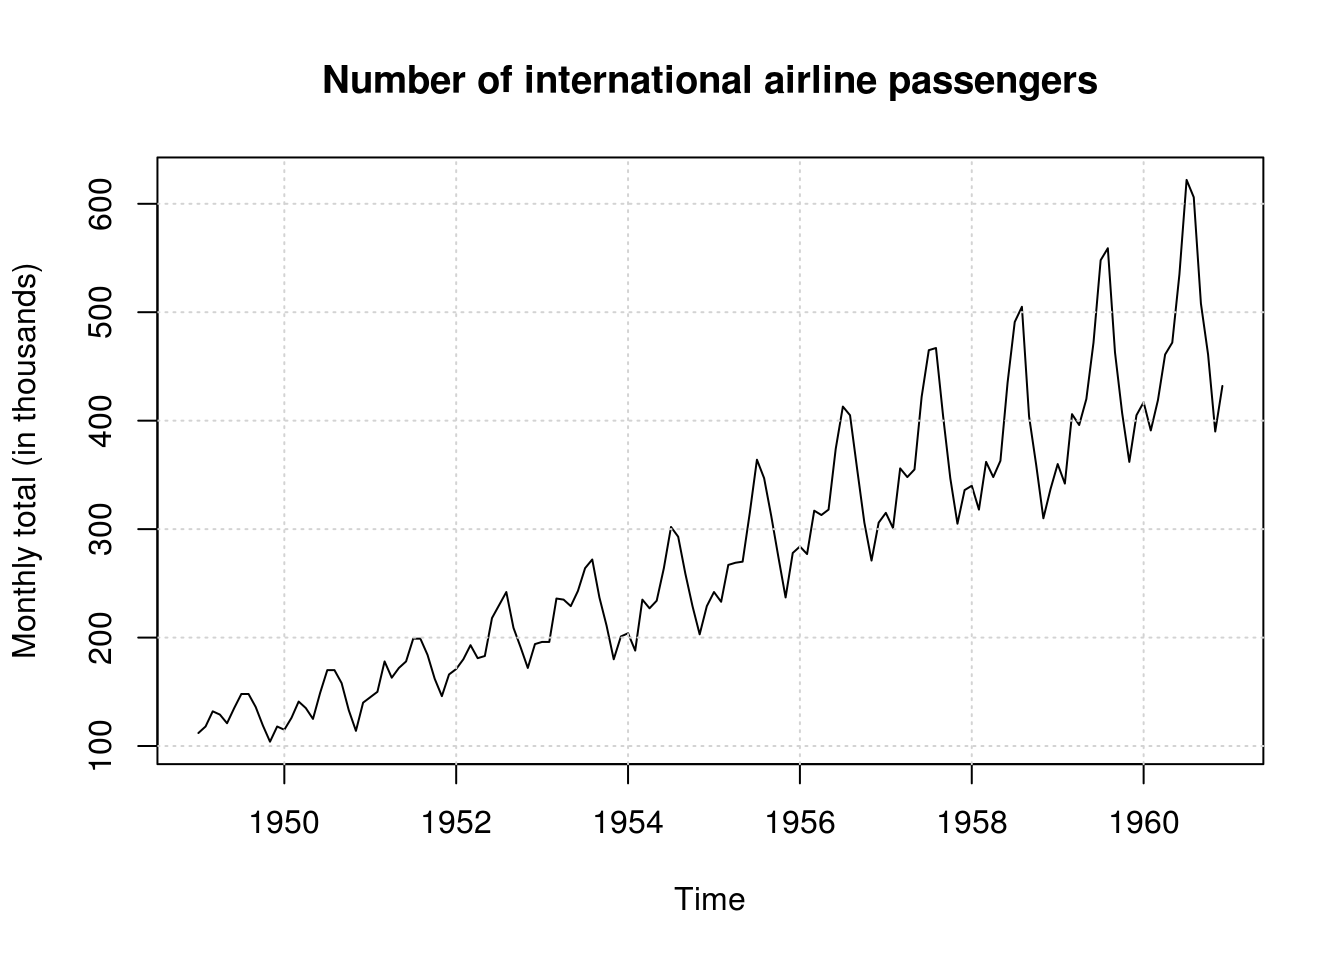
\includegraphics{timeseRies_files/figure-latex/AirPassenger-1.pdf}

\begin{Shaded}
\begin{Highlighting}[]
\StringTok{`}\DataTypeTok{?}\StringTok{`}\NormalTok{(sunspot.month)}
\KeywordTok{plot}\NormalTok{(sunspot.month, }\DataTypeTok{ylab =} \StringTok{"Monthly number of sunspots"}\NormalTok{, }\DataTypeTok{main =} \StringTok{"Monthly mean relative sunspot numbers from 1749 to 1983"}\NormalTok{, }
    \DataTypeTok{bty =} \StringTok{"l"}\NormalTok{)}
\end{Highlighting}
\end{Shaded}

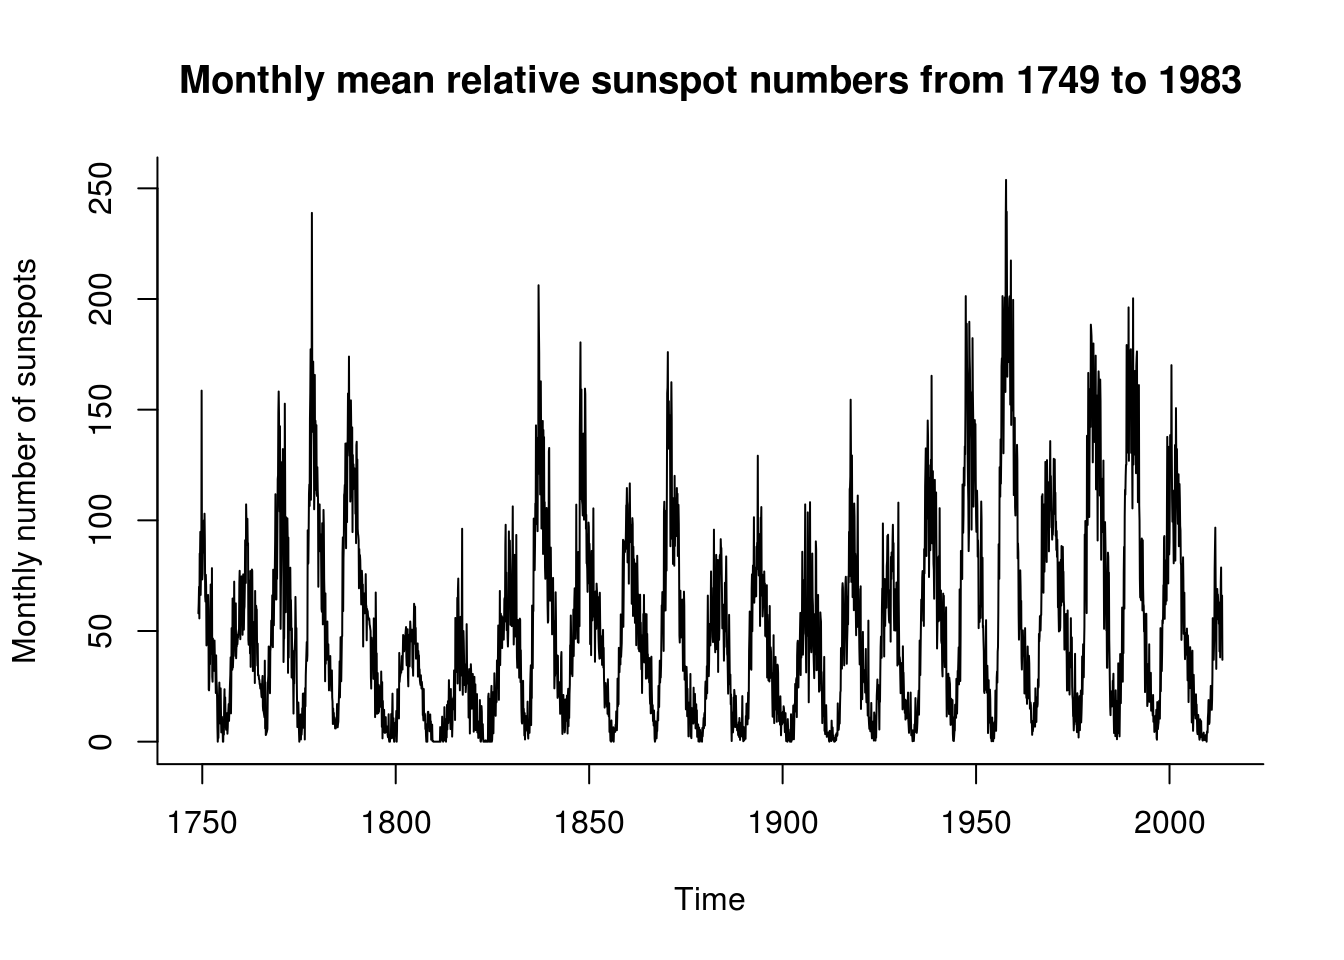
\includegraphics{timeseRies_files/figure-latex/AirPassenger-2.pdf}

\begin{Shaded}
\begin{Highlighting}[]
\CommentTok{# Dataset present in a R package - without loading the package}
\KeywordTok{data}\NormalTok{(}\DataTypeTok{list =} \StringTok{"birth"}\NormalTok{, }\DataTypeTok{package =} \StringTok{"astsa"}\NormalTok{)}
\KeywordTok{plot}\NormalTok{(birth, }\DataTypeTok{ylab =} \StringTok{"Monthly live births (in thousands)"}\NormalTok{, }\DataTypeTok{main =} \StringTok{"U.S. Monthly Live Birth"}\NormalTok{)}
\end{Highlighting}
\end{Shaded}

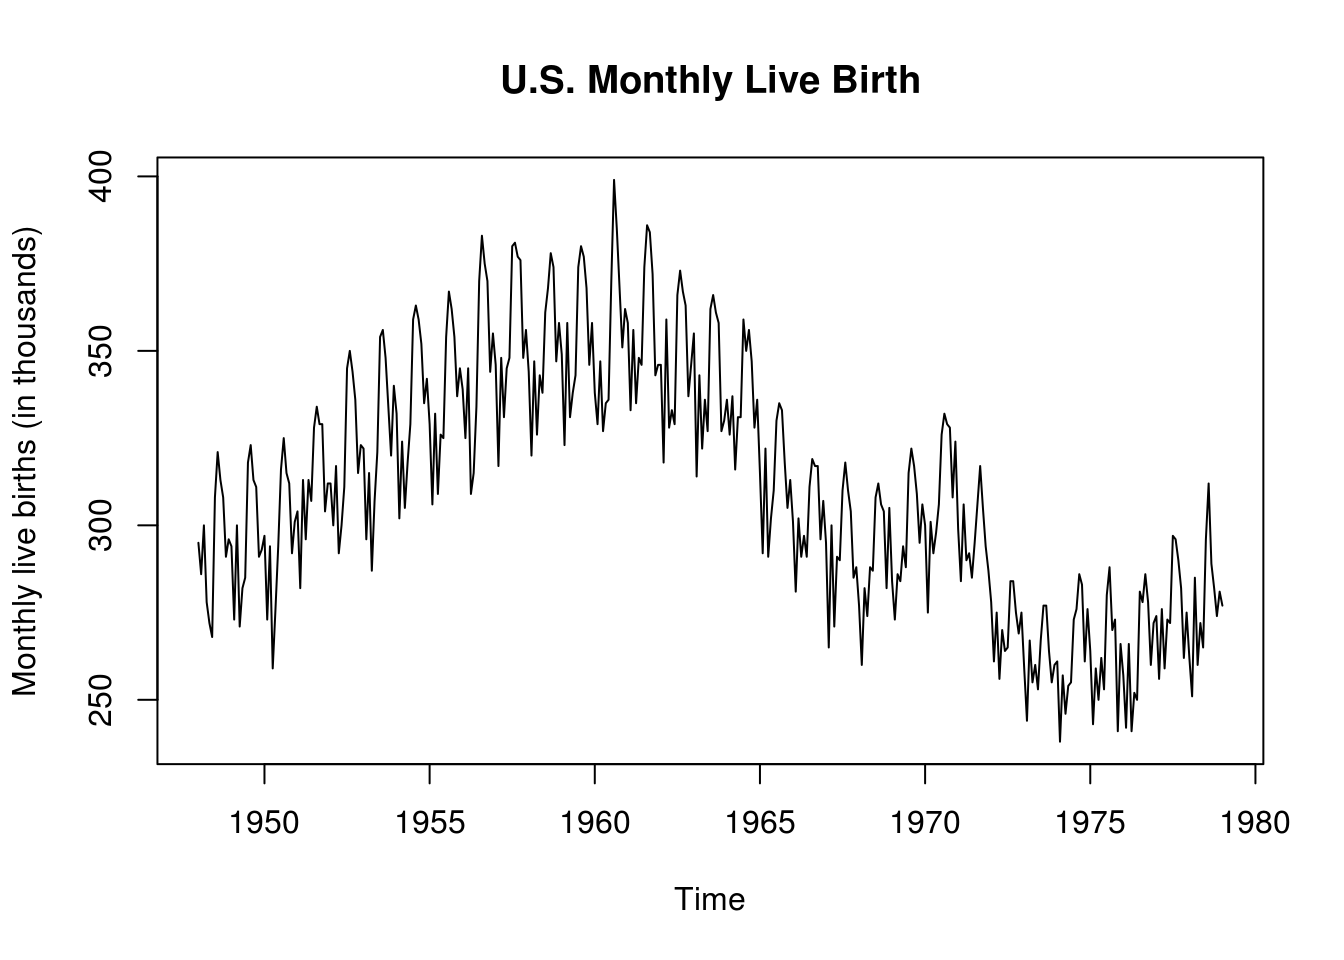
\includegraphics{timeseRies_files/figure-latex/AirPassenger-3.pdf}

\section{Introduction to the basic time series
functions}\label{introduction-to-the-basic-time-series-functions}

The first example we are going to handle is \texttt{lh}, a time series
of 48 observations at 10-minute intervals on luteinizing hormone levels
for a human female. Start by printing it.

\begin{Shaded}
\begin{Highlighting}[]
\NormalTok{lh}
\end{Highlighting}
\end{Shaded}

\begin{verbatim}
Time Series:
Start = 1 
End = 48 
Frequency = 1 
 [1] 2.4 2.4 2.4 2.2 2.1 1.5 2.3 2.3 2.5 2.0 1.9 1.7 2.2 1.8 3.2 3.2 2.7
[18] 2.2 2.2 1.9 1.9 1.8 2.7 3.0 2.3 2.0 2.0 2.9 2.9 2.7 2.7 2.3 2.6 2.4
[35] 1.8 1.7 1.5 1.4 2.1 3.3 3.5 3.5 3.1 2.6 2.1 3.4 3.0 2.9
\end{verbatim}

Look at the information: \texttt{Start\ =\ 1}, \texttt{End\ =\ 48} and
\texttt{Frequency\ =\ 1}.

The second example, \texttt{deaths}, gives monthly deaths in the UK from
a set of common lung diseases for the years 1974 to 1979.

\begin{Shaded}
\begin{Highlighting}[]
\KeywordTok{data}\NormalTok{(}\StringTok{"deaths"}\NormalTok{, }\DataTypeTok{package =} \StringTok{"MASS"}\NormalTok{)}
\NormalTok{deaths}
\end{Highlighting}
\end{Shaded}

\begin{verbatim}
      Jan  Feb  Mar  Apr  May  Jun  Jul  Aug  Sep  Oct  Nov  Dec
1974 3035 2552 2704 2554 2014 1655 1721 1524 1596 2074 2199 2512
1975 2933 2889 2938 2497 1870 1726 1607 1545 1396 1787 2076 2837
1976 2787 3891 3179 2011 1636 1580 1489 1300 1356 1653 2013 2823
1977 3102 2294 2385 2444 1748 1554 1498 1361 1346 1564 1640 2293
1978 2815 3137 2679 1969 1870 1633 1529 1366 1357 1570 1535 2491
1979 3084 2605 2573 2143 1693 1504 1461 1354 1333 1492 1781 1915
\end{verbatim}

Use \texttt{tsp(deaths)} to get \texttt{Start\ =\ 1974},
\texttt{End\ =\ 1979.917} and \texttt{Frequency\ =\ 12}. You can also
access each of these attributes using the functions
\texttt{start(deaths)}, \texttt{end(deaths)} and
\texttt{frequency(deaths)}. Use \texttt{cycle(deaths)} to get the
position in the cycle of each observation.

Time series can be plotted by \texttt{plot}. The argument \texttt{lty}
of the function \texttt{plot} controls the type of the plotted line
(solid, dashed, dotted, \ldots{}). For more details, type \texttt{?par}
(for graphical parameters).

\begin{Shaded}
\begin{Highlighting}[]
\KeywordTok{par}\NormalTok{(}\DataTypeTok{mfrow =} \KeywordTok{c}\NormalTok{(}\DecValTok{1}\NormalTok{, }\DecValTok{2}\NormalTok{))  }\CommentTok{#2 plot side by side}
\KeywordTok{plot}\NormalTok{(lh, }\DataTypeTok{main =} \StringTok{"Luteinizing Hormone in}\CharTok{\textbackslash{}n}\StringTok{Blood Samples"}\NormalTok{, }\DataTypeTok{ylab =} \StringTok{"IU/L"}\NormalTok{, }\DataTypeTok{xlab =} \StringTok{"Number of 10 minutes intervals}\CharTok{\textbackslash{}n}\StringTok{ from first sample"}\NormalTok{)}
\KeywordTok{plot}\NormalTok{(deaths, }\DataTypeTok{main =} \StringTok{"Monthly Deaths from }\CharTok{\textbackslash{}n}\StringTok{Lung Diseases in the UK"}\NormalTok{, }\DataTypeTok{ylab =} \StringTok{"Monthly deaths"}\NormalTok{, }
    \DataTypeTok{ylim =} \KeywordTok{c}\NormalTok{(}\DecValTok{0}\NormalTok{, }\DecValTok{4000}\NormalTok{))}
\KeywordTok{lines}\NormalTok{(mdeaths, }\DataTypeTok{lty =} \DecValTok{2}\NormalTok{)}
\KeywordTok{lines}\NormalTok{(fdeaths, }\DataTypeTok{lty =} \DecValTok{3}\NormalTok{)}
\KeywordTok{legend}\NormalTok{(}\DataTypeTok{x =} \StringTok{"topright"}\NormalTok{, }\DataTypeTok{bty =} \StringTok{"n"}\NormalTok{, }\DataTypeTok{legend =} \KeywordTok{c}\NormalTok{(}\StringTok{"Total"}\NormalTok{, }\StringTok{"Men"}\NormalTok{, }\StringTok{"Women"}\NormalTok{), }\DataTypeTok{lty =} \KeywordTok{c}\NormalTok{(}\DecValTok{1}\NormalTok{, }
    \DecValTok{2}\NormalTok{, }\DecValTok{3}\NormalTok{))}
\end{Highlighting}
\end{Shaded}

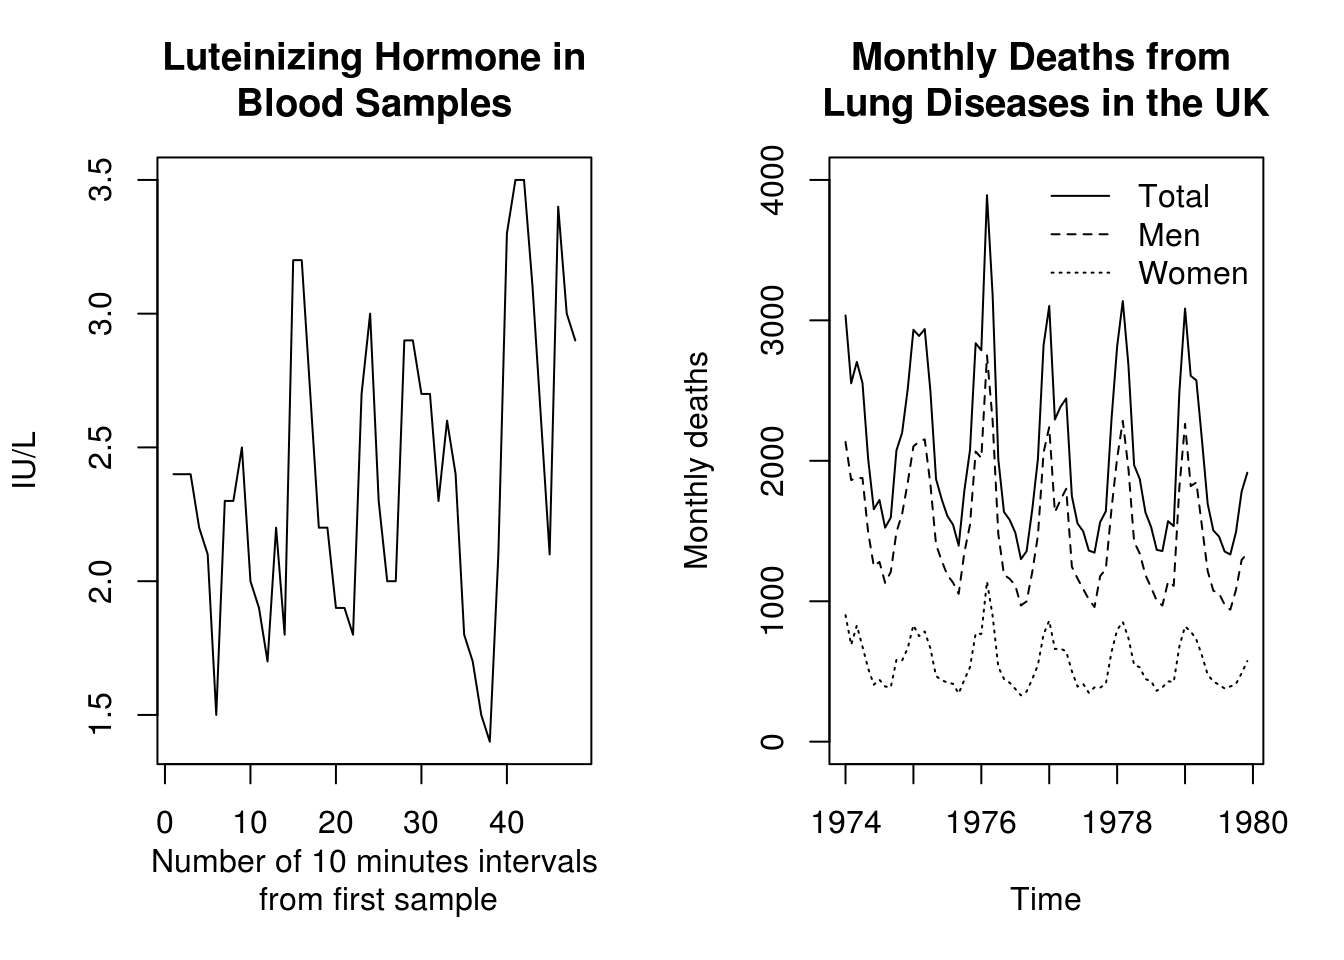
\includegraphics{timeseRies_files/figure-latex/basic_plots-1.pdf}

\begin{Shaded}
\begin{Highlighting}[]
\KeywordTok{graphics.off}\NormalTok{()  }\CommentTok{#close console}
\end{Highlighting}
\end{Shaded}

Above, you can see plots of \texttt{lh} and the three series on deaths.
In the right-hand plot, the dashed series is for males, the dotted
series for females and the solid line for the total.

The functions \texttt{ts.union} and \texttt{ts.intersect} bind together
multiple time series which have a common frequency. The time axes are
aligned and only observations at times that appear in all the series are
retained with \texttt{ts.intersect}; with \texttt{ts.union} the combined
series covers the whole range of the components, possibly as \texttt{NA}
values.

The function \texttt{window} extracts a sub-series of a single or
multiple time series, by specifying \texttt{start}, \texttt{end} or
both.

The function \texttt{lag} shifts the time axis of a series back by \(k\)
positions (default is \texttt{k\ =\ 1}). Thus \texttt{lag(deaths,\ k=3)}
is the series of deaths shifted one quarter into the past.

\begin{Shaded}
\begin{Highlighting}[]
\KeywordTok{plot}\NormalTok{(deaths, }\DataTypeTok{main =} \StringTok{"Monthly Deaths from }\CharTok{\textbackslash{}n}\StringTok{Lung Diseases in the UK"}\NormalTok{, }\DataTypeTok{ylab =} \StringTok{"Monthly deaths"}\NormalTok{, }
    \DataTypeTok{bty =} \StringTok{"l"}\NormalTok{)}
\KeywordTok{lines}\NormalTok{(}\KeywordTok{lag}\NormalTok{(deaths, }\DataTypeTok{k =} \DecValTok{3}\NormalTok{), }\DataTypeTok{lty =} \DecValTok{3}\NormalTok{)}
\end{Highlighting}
\end{Shaded}

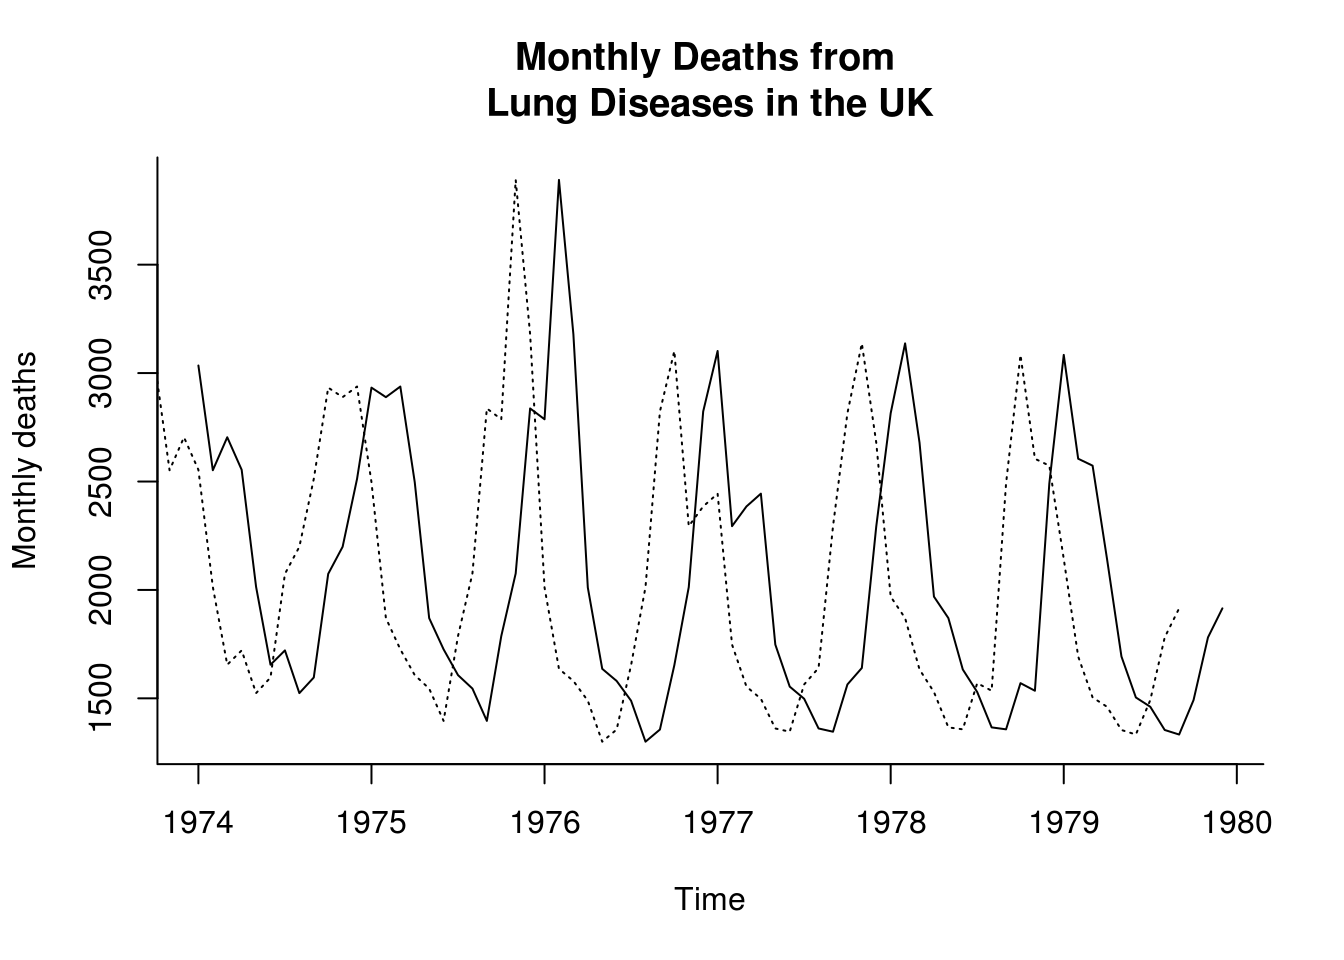
\includegraphics{timeseRies_files/figure-latex/unnamed-chunk-3-1.pdf}

The function \texttt{diff} takes the difference between a series and its
lagged values and so returns a series of length \(n-k\) with values lost
from the beginning (if \(k>0\)) or end. Beware: the argument
\texttt{lag} (default is \texttt{lag\ =\ 1}) is used in the usual sense
here, so \texttt{diff(deaths,\ lag=3)} is equal to
\texttt{deaths\ -\ lag(deaths,\ k=-3)}! The function \texttt{diff} has
an argument \texttt{differences} which causes the operation to be
iterated.

The function \texttt{aggregate} can be used to change the frequency of
the time base.

\begin{Shaded}
\begin{Highlighting}[]
\KeywordTok{aggregate}\NormalTok{(deaths, }\DecValTok{4}\NormalTok{, sum)}
\end{Highlighting}
\end{Shaded}

\begin{verbatim}
     Qtr1 Qtr2 Qtr3 Qtr4
1974 8291 6223 4841 6785
1975 8760 6093 4548 6700
1976 9857 5227 4145 6489
1977 7781 5746 4205 5497
1978 8631 5472 4252 5596
1979 8262 5340 4148 5188
\end{verbatim}

\begin{Shaded}
\begin{Highlighting}[]
\KeywordTok{aggregate}\NormalTok{(deaths, }\DecValTok{1}\NormalTok{, sum)}
\end{Highlighting}
\end{Shaded}

\begin{verbatim}
Time Series:
Start = 1974 
End = 1979 
Frequency = 1 
[1] 26140 26101 25718 23229 23951 22938
\end{verbatim}

\begin{Shaded}
\begin{Highlighting}[]
\KeywordTok{aggregate}\NormalTok{(deaths, }\DecValTok{4}\NormalTok{, mean)}
\end{Highlighting}
\end{Shaded}

\begin{verbatim}
         Qtr1     Qtr2     Qtr3     Qtr4
1974 2763.667 2074.333 1613.667 2261.667
1975 2920.000 2031.000 1516.000 2233.333
1976 3285.667 1742.333 1381.667 2163.000
1977 2593.667 1915.333 1401.667 1832.333
1978 2877.000 1824.000 1417.333 1865.333
1979 2754.000 1780.000 1382.667 1729.333
\end{verbatim}

\begin{Shaded}
\begin{Highlighting}[]
\KeywordTok{aggregate}\NormalTok{(deaths, }\DecValTok{1}\NormalTok{, mean)}
\end{Highlighting}
\end{Shaded}

\begin{verbatim}
Time Series:
Start = 1974 
End = 1979 
Frequency = 1 
[1] 2178.333 2175.083 2143.167 1935.750 1995.917 1911.500
\end{verbatim}

One way to compute the linear or polynomial trend of a series is to use
the function \texttt{lm}, which fits linear models. The function
\texttt{fitted} allows you to extract the model fitted values, while
\texttt{c(1:48)} represents the integers from 1 to 48 and the function
\texttt{poly} computes orthogonal polynomials.

\begin{Shaded}
\begin{Highlighting}[]
\KeywordTok{plot}\NormalTok{(lh, }\DataTypeTok{main =} \StringTok{"Luteinizing Hormone in Blood Samples"}\NormalTok{, }\DataTypeTok{ylab =} \StringTok{"IU/L"}\NormalTok{, }\DataTypeTok{xlab =} \StringTok{"Number of 10 minutes intervals}\CharTok{\textbackslash{}n}\StringTok{ from first sample"}\NormalTok{, }
    \DataTypeTok{bty =} \StringTok{"l"}\NormalTok{, }\DataTypeTok{ylim =} \KeywordTok{c}\NormalTok{(}\DecValTok{0}\NormalTok{, }\FloatTok{3.5}\NormalTok{))}
\KeywordTok{lines}\NormalTok{(}\KeywordTok{fitted}\NormalTok{(}\KeywordTok{lm}\NormalTok{(lh }\OperatorTok{~}\StringTok{ }\KeywordTok{c}\NormalTok{(}\DecValTok{1}\OperatorTok{:}\DecValTok{48}\NormalTok{))), }\DataTypeTok{col =} \StringTok{"blue"}\NormalTok{)}
\KeywordTok{lines}\NormalTok{(}\KeywordTok{fitted}\NormalTok{(}\KeywordTok{lm}\NormalTok{(lh }\OperatorTok{~}\StringTok{ }\KeywordTok{poly}\NormalTok{(}\DecValTok{1}\OperatorTok{:}\DecValTok{48}\NormalTok{, }\DecValTok{2}\NormalTok{))), }\DataTypeTok{col =} \StringTok{"red"}\NormalTok{)}
\KeywordTok{legend}\NormalTok{(}\DataTypeTok{x =} \StringTok{"bottomright"}\NormalTok{, }\DataTypeTok{legend =} \KeywordTok{c}\NormalTok{(}\StringTok{"linear"}\NormalTok{, }\StringTok{"quadratic"}\NormalTok{), }\DataTypeTok{col =} \KeywordTok{c}\NormalTok{(}\DecValTok{4}\NormalTok{, }\DecValTok{2}\NormalTok{), }
    \DataTypeTok{lty =} \KeywordTok{c}\NormalTok{(}\DecValTok{1}\NormalTok{, }\DecValTok{1}\NormalTok{), }\DataTypeTok{bty =} \StringTok{"n"}\NormalTok{)}
\end{Highlighting}
\end{Shaded}

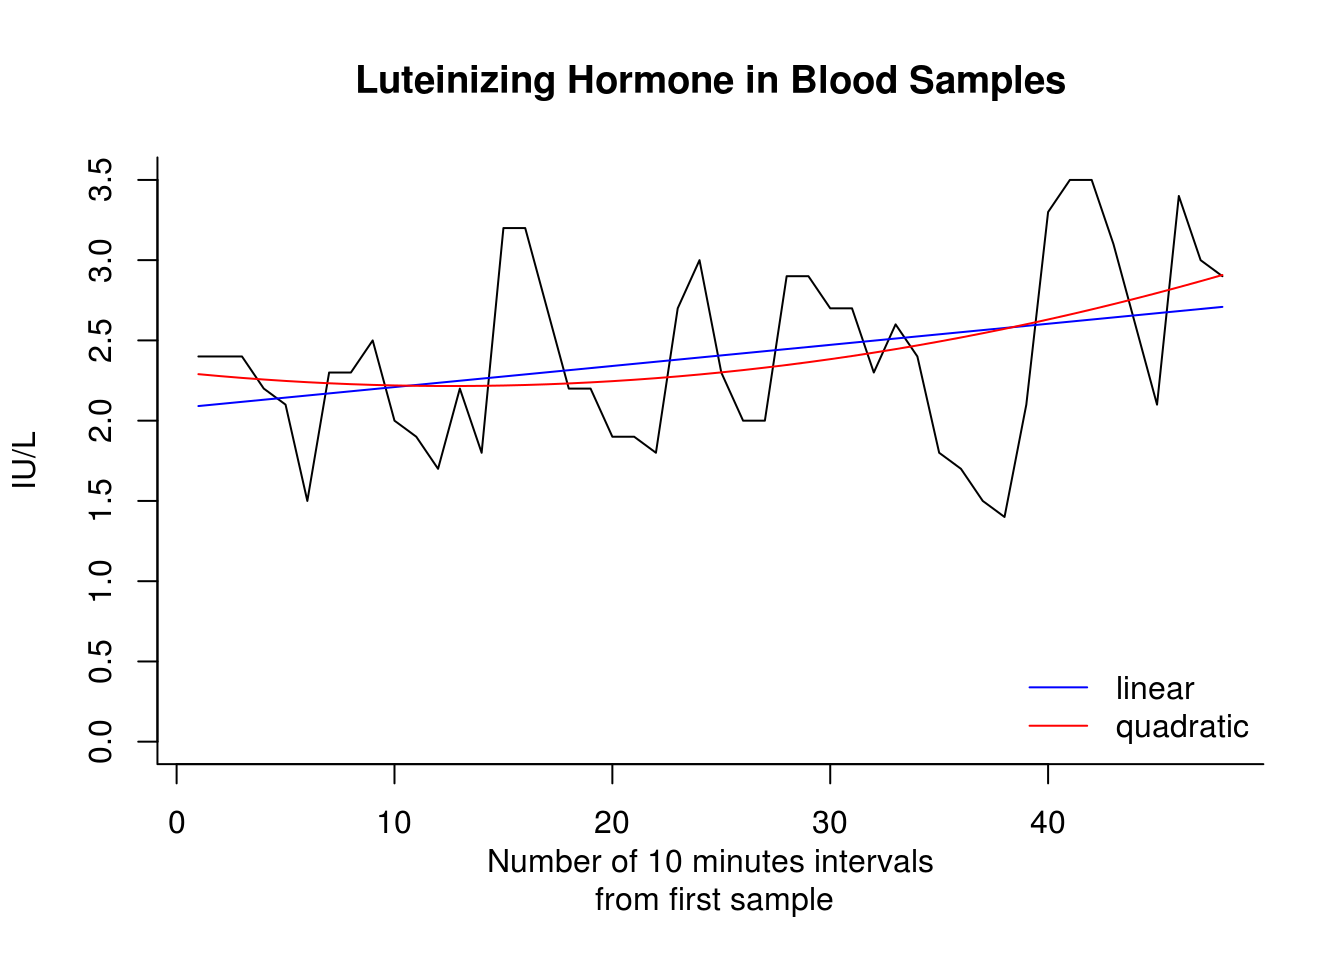
\includegraphics{timeseRies_files/figure-latex/unnamed-chunk-5-1.pdf}

\subsection{Exercise 1: Beaver
temperature}\label{exercise-1-beaver-temperature}

\begin{enumerate}
\def\labelenumi{\arabic{enumi}.}
\tightlist
\item
  Load the \texttt{beav2} data from the library \texttt{MASS}.
\item
  Examine the data frame using \texttt{summary}, \texttt{head},
  \texttt{tail}. Query the help with \texttt{?beav2} for a description
  of the dataset
\item
  Transform the temperature data into a time series object and plot the
  latter.
\item
  Fit a linear model using \texttt{lm} and the variable \texttt{activ}
  as factor, viz.
  \texttt{lin\_mod\ \textless{}-\ lm(temp\textasciitilde{}as.factor(activ),\ data=beav2)}.
  Overlay the means on your plot with \texttt{lines(fitted(lin\_mod))}
  replacing \texttt{lin\_mod} with your \texttt{lm} result.
\item
  Inspect the residuals (\texttt{resid(lin\_mod)}) and determine whether
  there is any evidence of trend or seasonality.
\item
  Look at a quantile-quantile (Q-Q) plot to assess normality. You can
  use the command \texttt{qqnorm} if you don't want to transform
  manually the residuals with \texttt{qqline} or use
  \texttt{plot(lin\_mod,\ which=2)}.
\item
  Plot the lag-one residuals at time \(t\) and \(t-1\). Is the
  dependence approximately linear?
\end{enumerate}

\section{Second order stationarity}\label{second-order-stationarity}

The example below corresponds to examples 1.9 and 1.10 from Shumway and
Stoffer. It shows how to create MA and AR series based on white noise
using the \texttt{filter} function. It is best practice when simulating
autoregressive models to burn-in (discard) the first few iterations to
remove the dependencies on the starting values (here zeros). Note that
the function \texttt{filter} returns a \texttt{ts} object.

\begin{Shaded}
\begin{Highlighting}[]
\KeywordTok{set.seed}\NormalTok{(}\DecValTok{1}\NormalTok{)}
\NormalTok{x <-}\StringTok{ }\KeywordTok{rnorm}\NormalTok{(}\DecValTok{550}\NormalTok{, }\DecValTok{0}\NormalTok{, }\DecValTok{1}\NormalTok{)  }\CommentTok{# Samples from N(0,1) variates}
\NormalTok{y <-}\StringTok{ }\KeywordTok{filter}\NormalTok{(x, }\DataTypeTok{method =} \StringTok{"recursive"}\NormalTok{, }\DataTypeTok{filter =} \KeywordTok{c}\NormalTok{(}\DecValTok{1}\NormalTok{, }\OperatorTok{-}\FloatTok{0.9}\NormalTok{))  }\CommentTok{#autoregression}
\NormalTok{z <-}\StringTok{ }\KeywordTok{filter}\NormalTok{(x, }\DataTypeTok{method =} \StringTok{"convolution"}\NormalTok{, }\DataTypeTok{filter =} \KeywordTok{rep}\NormalTok{(}\DecValTok{1}\OperatorTok{/}\DecValTok{3}\NormalTok{, }\DecValTok{3}\NormalTok{), }\DataTypeTok{sides =} \DecValTok{2}\NormalTok{)  }\CommentTok{# moving average}
\KeywordTok{class}\NormalTok{(z)}
\end{Highlighting}
\end{Shaded}

\begin{verbatim}
[1] "ts"
\end{verbatim}

\begin{Shaded}
\begin{Highlighting}[]
\NormalTok{x <-}\StringTok{ }\NormalTok{x[}\OperatorTok{-}\KeywordTok{c}\NormalTok{(}\DecValTok{1}\OperatorTok{:}\DecValTok{49}\NormalTok{, }\DecValTok{550}\NormalTok{)]}
\NormalTok{y <-}\StringTok{ }\NormalTok{y[}\OperatorTok{-}\KeywordTok{c}\NormalTok{(}\DecValTok{1}\OperatorTok{:}\DecValTok{49}\NormalTok{, }\DecValTok{550}\NormalTok{)]}
\NormalTok{z <-}\StringTok{ }\NormalTok{z[}\OperatorTok{-}\KeywordTok{c}\NormalTok{(}\DecValTok{1}\OperatorTok{:}\DecValTok{49}\NormalTok{, }\DecValTok{550}\NormalTok{)]}
\CommentTok{# ts.union if we did not remove values (and the class `ts`)}
\KeywordTok{plot.ts}\NormalTok{(}\KeywordTok{cbind}\NormalTok{(x, y, z), }\DataTypeTok{main =} \StringTok{"Simulated time series"}\NormalTok{)}
\end{Highlighting}
\end{Shaded}

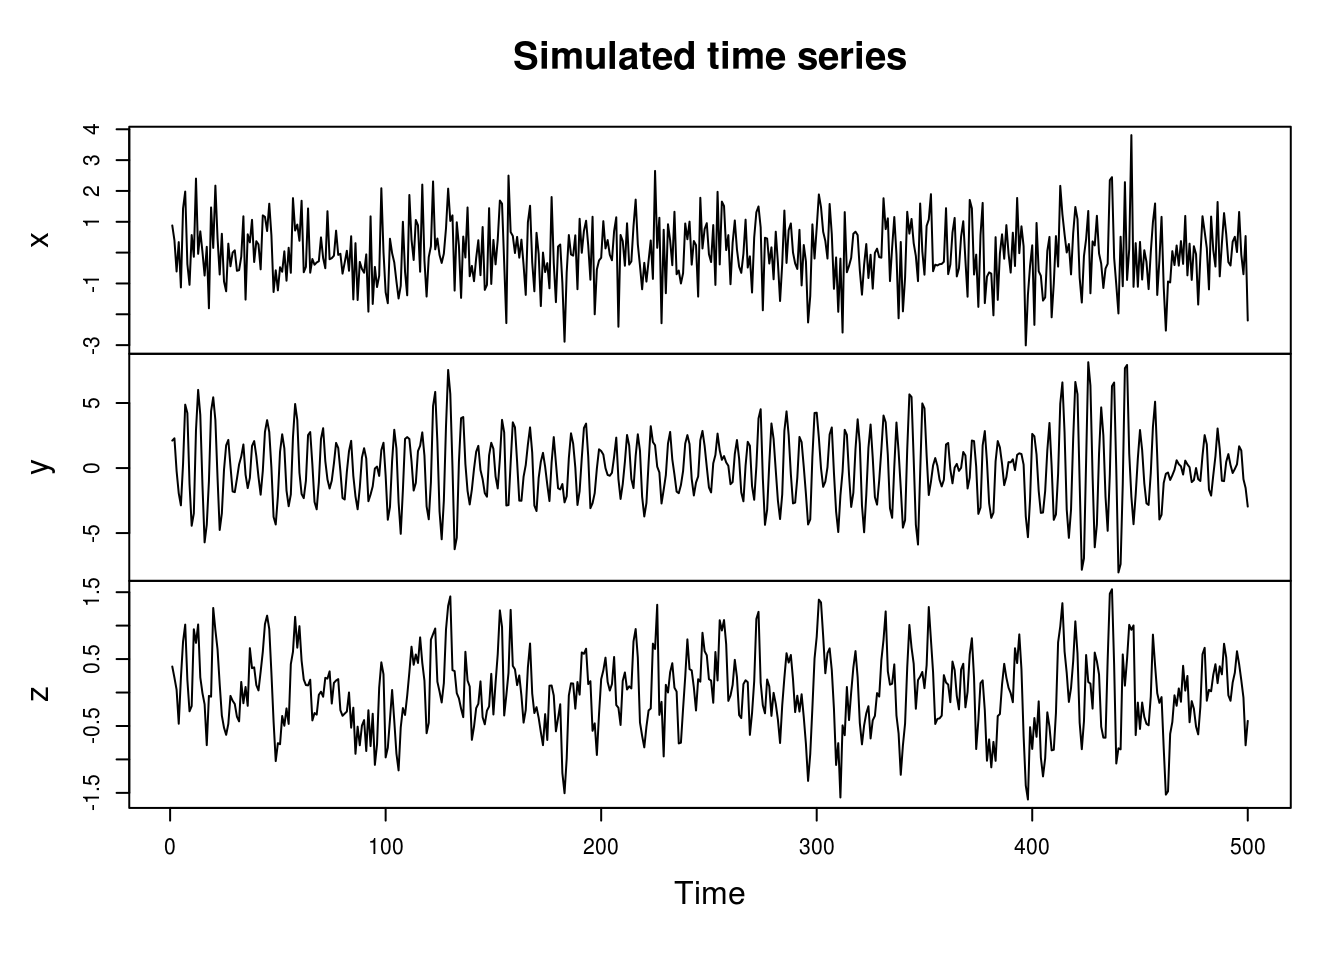
\includegraphics{timeseRies_files/figure-latex/2nd_order_statio-1.pdf}

We notice immediately that the MA process looks smoother than the white
noise, and that the innovations (peaks) of the AR process are longer
lasting. If we had not simulated more values and kept some, the first
and last observations of \(z\) would be \texttt{NA}s. The series created
are of the form \[ z_t=\frac{1}{3}(x_{t-1}+x_{t}+x_{t+1})\] and
\[ y_t= y_{t-1}-0.9y_{t-2}+x_t.\]

The correlogram provides an easy to use summary for detecting
\emph{linear} dependencies based on correlations. The function
\texttt{acf} will return a plot of the correlogram, by default using the
correlation. Unfortunately, the basic graph starts at lag 1, which by
default has correlation 1 and thus compress the whole plot
unnecessarily. Blue dashed lines indicate 5\% critical values at
\(\pm 1.96/\sqrt{n}\) under the null hypothesis of white noise
(\emph{not} stationarity).

The function \texttt{acf} computes and plots \(c_t\) and \(r_t\), the
estimators for the autocovariance and autocorrelation functions
\[c_t= n^{-1}\sum_{s=\max(1,-t)}^{\min(n-t,n)}[X_{s+t}-\bar X][X_s-\bar X], \quad r_t={c_t}/{c_0}.\]
The argument \texttt{type} controls which is used and defaults to the
correlation. This is easily extended to several time series observed
over the same interval
\[c_{ij}(t) = n^{-1}\sum_{s=\max(1,-t)}^{\min(n-t,n)}[X_i(s+t)-\bar X_i][X_j(s)-\bar X_j].\]

Unfortunately, the function \texttt{acf} always display the zero-lag
autocorrelation, which is 1 by definition. This oftentimes squeezes the
whole correlogram values and requires manual adjustment so one can
properly view whether the sample autocorrelations are significant.

\begin{Shaded}
\begin{Highlighting}[]
\CommentTok{# acf(x, lag.max=20, demean = TRUE, main = 'White noise') #WRONG}
\KeywordTok{par}\NormalTok{(}\DataTypeTok{mfrow =} \KeywordTok{c}\NormalTok{(}\DecValTok{1}\NormalTok{, }\DecValTok{2}\NormalTok{))}
\NormalTok{TSA}\OperatorTok{::}\KeywordTok{acf}\NormalTok{(x, }\DataTypeTok{demean =} \OtherTok{TRUE}\NormalTok{, }\DataTypeTok{main =} \StringTok{"White noise"}\NormalTok{)}
\KeywordTok{pacf}\NormalTok{(x, }\DataTypeTok{lag.max =} \DecValTok{20}\NormalTok{, }\DataTypeTok{main =} \StringTok{"White noise"}\NormalTok{)}
\end{Highlighting}
\end{Shaded}

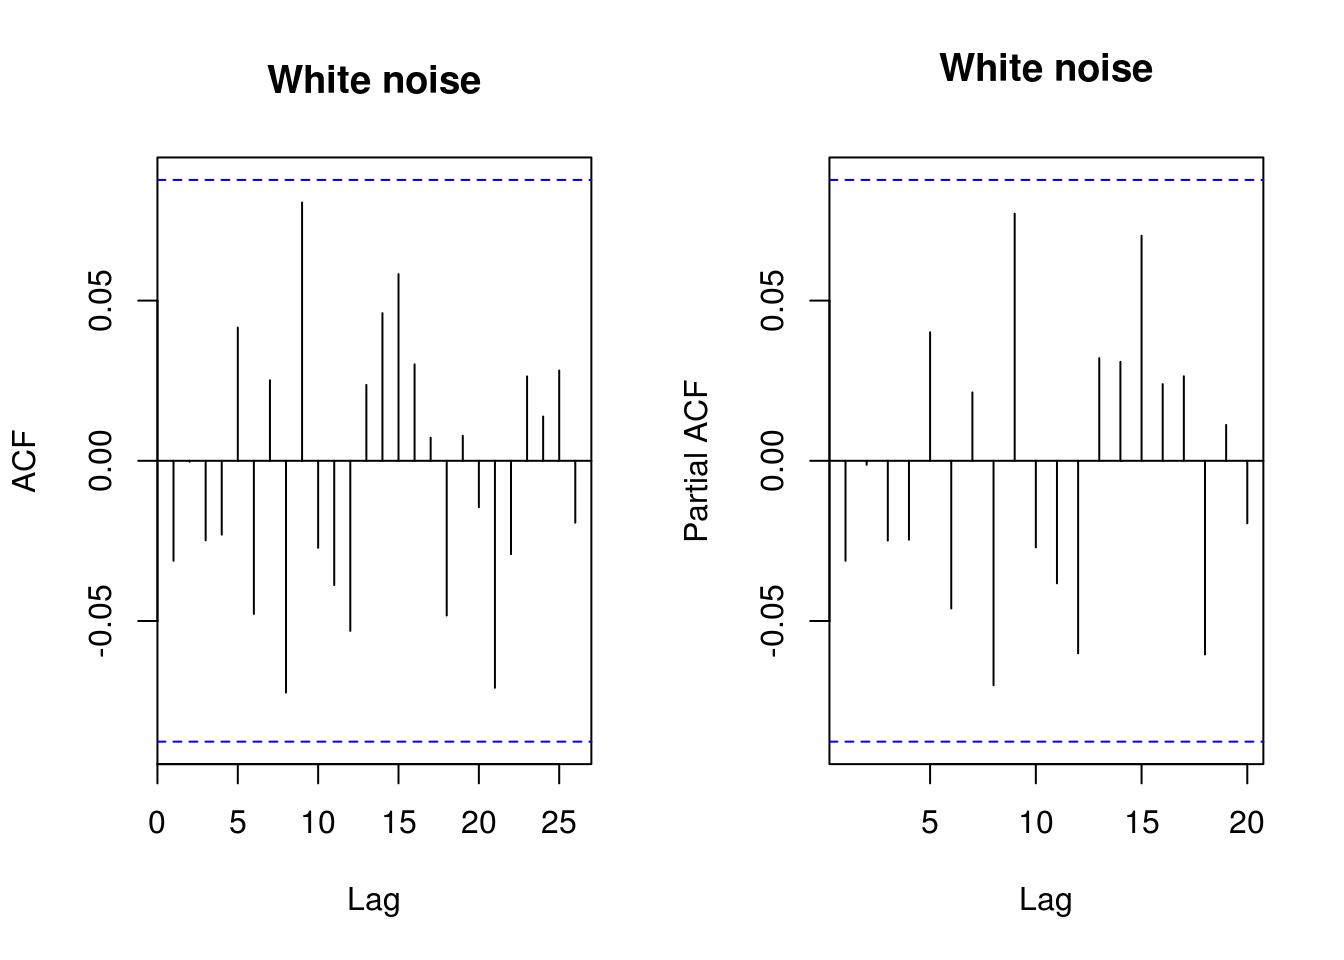
\includegraphics{timeseRies_files/figure-latex/acf_plots1-1.pdf}

\begin{Shaded}
\begin{Highlighting}[]
\CommentTok{# Equivalent functions from forecast}
\NormalTok{forecast}\OperatorTok{::}\KeywordTok{Acf}\NormalTok{(y, }\DataTypeTok{main =} \StringTok{"Autoregressive process"}\NormalTok{)}
\NormalTok{forecast}\OperatorTok{::}\KeywordTok{Acf}\NormalTok{(y, }\DataTypeTok{type =} \StringTok{"partial"}\NormalTok{, }\DataTypeTok{main =} \StringTok{"Autoregressive process"}\NormalTok{)  }\CommentTok{#or forecast::Pacf}
\end{Highlighting}
\end{Shaded}

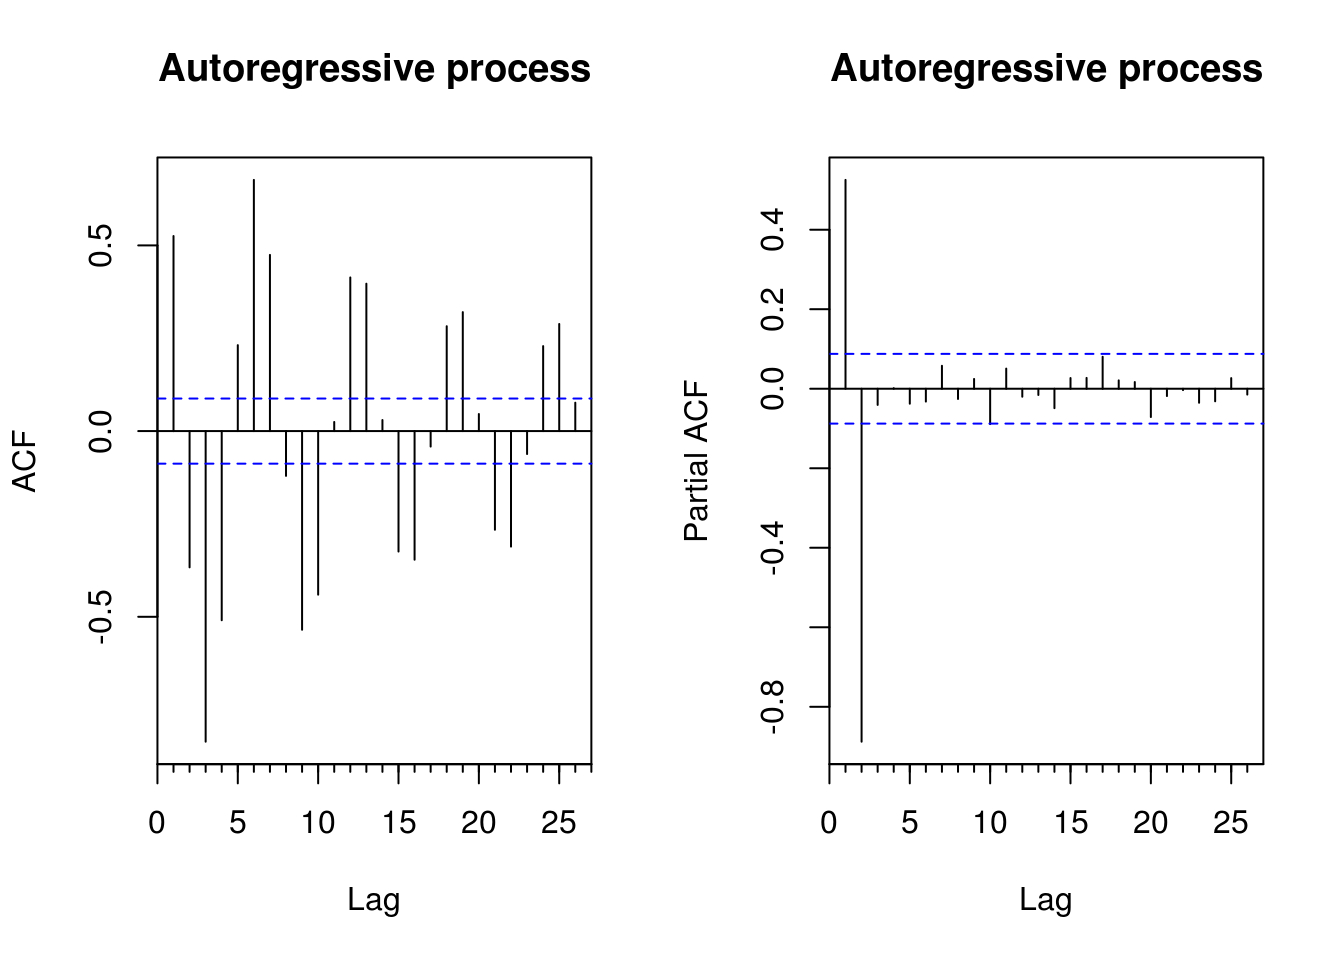
\includegraphics{timeseRies_files/figure-latex/acf_plots1-2.pdf}

You can thus use instead the function \texttt{forecast::Acf}, which
removes the first lag of the autocorrelation function plot, or
\texttt{TSA::acf}. The function \texttt{pacf} return the partial
autocorrelations and the function \texttt{ccf} to compute the
cross-correlation or cross-covariance of two univariate series

\begin{Shaded}
\begin{Highlighting}[]
\CommentTok{# Load datasets}
\KeywordTok{data}\NormalTok{(deaths, }\DataTypeTok{package =} \StringTok{"MASS"}\NormalTok{)}
\KeywordTok{data}\NormalTok{(lh, }\DataTypeTok{package =} \StringTok{"datasets"}\NormalTok{)}
\CommentTok{# Second order summaries}
\NormalTok{forecast}\OperatorTok{::}\KeywordTok{Acf}\NormalTok{(lh, }\DataTypeTok{main =} \StringTok{"Correlogram of }\CharTok{\textbackslash{}n}\StringTok{Luteinizing Hormone"}\NormalTok{, }\DataTypeTok{ylab =} \StringTok{"Autocorrelation"}\NormalTok{)  }\CommentTok{#autocorrelation}
\KeywordTok{acf}\NormalTok{(lh, }\DataTypeTok{type =} \StringTok{"covariance"}\NormalTok{, }\DataTypeTok{main =} \StringTok{"Autocovariance of}\CharTok{\textbackslash{}n}\StringTok{ Luteinizing Hormone"}\NormalTok{)  }\CommentTok{#autocovariance}
\KeywordTok{acf}\NormalTok{(deaths, }\DataTypeTok{main =} \StringTok{"Correlogram of}\CharTok{\textbackslash{}n}\StringTok{`deaths` dataset"}\NormalTok{)}
\KeywordTok{ccf}\NormalTok{(fdeaths, mdeaths, }\DataTypeTok{ylab =} \StringTok{"cross-correlation"}\NormalTok{, }\DataTypeTok{main =} \StringTok{"Cross correlation of `deaths` }\CharTok{\textbackslash{}n}\StringTok{female vs male"}\NormalTok{)}
\CommentTok{# acf(ts.union(mdeaths,fdeaths)) # acf and ccf - multiple time series of}
\CommentTok{# male and female deaths}
\end{Highlighting}
\end{Shaded}

The plots of the \texttt{deaths} series shows the pattern of seasonal
series, and the autocorrelations do not damp down for large lags. Note
how one of the cross series is only plotted for negative lags. Plot in
row 2 column 1 shows \(c_{12}\) for negative lags, a reflection of the
plot of \(c_{21}\) for positive lags. For the cross-correlation, use
e.g. \texttt{ccf(mdeaths,\ fdeaths,\ ylab="cross-correlation")}.

Plotting lagged residuals is a useful graphical diagnostic for detecting
non-linear dependencies. The following function plots residuals at \(k\)
different lags and may be useful for diagnostic purposes.

\begin{Shaded}
\begin{Highlighting}[]
\NormalTok{pairs.ts <-}\StringTok{ }\ControlFlowTok{function}\NormalTok{(d, }\DataTypeTok{lag.max =} \DecValTok{10}\NormalTok{) \{}
\NormalTok{    old_par <-}\StringTok{ }\KeywordTok{par}\NormalTok{(}\DataTypeTok{no.readonly =} \OtherTok{TRUE}\NormalTok{)}
\NormalTok{    n <-}\StringTok{ }\KeywordTok{length}\NormalTok{(d)}
\NormalTok{    X <-}\StringTok{ }\KeywordTok{matrix}\NormalTok{(}\OtherTok{NA}\NormalTok{, n }\OperatorTok{-}\StringTok{ }\NormalTok{lag.max, lag.max)}
\NormalTok{    col.names <-}\StringTok{ }\KeywordTok{paste}\NormalTok{(}\StringTok{"Time+"}\NormalTok{, }\DecValTok{1}\OperatorTok{:}\NormalTok{lag.max)}
    \ControlFlowTok{for}\NormalTok{ (i }\ControlFlowTok{in} \DecValTok{1}\OperatorTok{:}\NormalTok{lag.max) X[, i] <-}\StringTok{ }\NormalTok{d[i }\OperatorTok{-}\StringTok{ }\DecValTok{1} \OperatorTok{+}\StringTok{ }\DecValTok{1}\OperatorTok{:}\NormalTok{(n }\OperatorTok{-}\StringTok{ }\NormalTok{lag.max)]}
    \KeywordTok{par}\NormalTok{(}\DataTypeTok{mfrow =} \KeywordTok{c}\NormalTok{(}\DecValTok{3}\NormalTok{, }\DecValTok{3}\NormalTok{), }\DataTypeTok{pty =} \StringTok{"s"}\NormalTok{, }\DataTypeTok{mar =} \KeywordTok{c}\NormalTok{(}\DecValTok{3}\NormalTok{, }\DecValTok{4}\NormalTok{, }\FloatTok{0.5}\NormalTok{, }\FloatTok{0.5}\NormalTok{))}
\NormalTok{    lims <-}\StringTok{ }\KeywordTok{range}\NormalTok{(X)}
    \ControlFlowTok{for}\NormalTok{ (i }\ControlFlowTok{in} \DecValTok{2}\OperatorTok{:}\NormalTok{lag.max) }\KeywordTok{plot}\NormalTok{(X[, }\DecValTok{1}\NormalTok{], X[, i], }\DataTypeTok{panel.first =}\NormalTok{ \{}
        \KeywordTok{abline}\NormalTok{(}\DecValTok{0}\NormalTok{, }\DecValTok{1}\NormalTok{, }\DataTypeTok{col =} \StringTok{"grey"}\NormalTok{)}
\NormalTok{    \}, }\DataTypeTok{xlab =} \StringTok{"Time"}\NormalTok{, }\DataTypeTok{ylab =}\NormalTok{ col.names[i }\OperatorTok{-}\StringTok{ }\DecValTok{1}\NormalTok{], }\DataTypeTok{xlim =}\NormalTok{ lims, }\DataTypeTok{ylim =}\NormalTok{ lims, }\DataTypeTok{pch =} \DecValTok{20}\NormalTok{, }
        \DataTypeTok{col =} \KeywordTok{rgb}\NormalTok{(}\DecValTok{0}\NormalTok{, }\DecValTok{0}\NormalTok{, }\DecValTok{0}\NormalTok{, }\FloatTok{0.25}\NormalTok{))}
    \KeywordTok{par}\NormalTok{(old_par)}
\NormalTok{\}}
\CommentTok{# Look at lag k residuals}
\KeywordTok{pairs.ts}\NormalTok{(sunspots)}
\end{Highlighting}
\end{Shaded}

\subsection{Exercise 2: SP500 daily
returns}\label{exercise-2-sp500-daily-returns}

\begin{enumerate}
\def\labelenumi{\arabic{enumi}.}
\tightlist
\item
  Download the dataset using the following command
\end{enumerate}

\begin{Shaded}
\begin{Highlighting}[]
\NormalTok{sp500 <-}\StringTok{ }\NormalTok{tseries}\OperatorTok{::}\KeywordTok{get.hist.quote}\NormalTok{(}\DataTypeTok{instrument =} \StringTok{"^GSPC"}\NormalTok{, }\DataTypeTok{start =} \StringTok{"2000-01-01"}\NormalTok{, }
    \DataTypeTok{end =} \StringTok{"2016-12-31"}\NormalTok{, }\DataTypeTok{quote =} \StringTok{"AdjClose"}\NormalTok{, }\DataTypeTok{provider =} \StringTok{"yahoo"}\NormalTok{, }\DataTypeTok{origin =} \StringTok{"1970-01-01"}\NormalTok{, }
    \DataTypeTok{compression =} \StringTok{"d"}\NormalTok{, }\DataTypeTok{retclass =} \StringTok{"zoo"}\NormalTok{)}
\end{Highlighting}
\end{Shaded}

\begin{enumerate}
\def\labelenumi{\arabic{enumi}.}
\setcounter{enumi}{1}
\tightlist
\item
  Obtain the daily percent return series and plot the latter against
  time.
\item
  With the help of graphs, discuss evidences of seasonality and
  nonstationarity. Are there seasons of returns?
\item
  Plot the (partial) correlogram of both the raw and the return series.
  Try the acf with \texttt{na.action=na.pass} and without (by
  e.g.~converting the series to a vector using \texttt{as.vector}.
  Comment on the impact of ignoring time stamps.
\item
  Plot the (partial) correlogram of the absolute value of the return
  series and of the squared return series. What do you see?
\end{enumerate}

\section{Simulations}\label{simulations}

The workhorse for simulations from ARIMA models is \texttt{arima.sim}.
To generate an AR(1) and an MA(1) processes using the function
\texttt{arima.sim}, one can use.

\begin{Shaded}
\begin{Highlighting}[]
\NormalTok{ar1 <-}\StringTok{ }\KeywordTok{arima.sim}\NormalTok{(}\DataTypeTok{n =} \DecValTok{100}\NormalTok{, }\DataTypeTok{model =} \KeywordTok{list}\NormalTok{(}\DataTypeTok{ar =} \FloatTok{0.9}\NormalTok{))}
\NormalTok{ma1 <-}\StringTok{ }\KeywordTok{arima.sim}\NormalTok{(}\DataTypeTok{n =} \DecValTok{100}\NormalTok{, }\DataTypeTok{model =} \KeywordTok{list}\NormalTok{(}\DataTypeTok{ma =} \FloatTok{0.8}\NormalTok{))}
\end{Highlighting}
\end{Shaded}

Define the following function to generate an ARCH(1) process.

\begin{Shaded}
\begin{Highlighting}[]
\NormalTok{arch.sim1 <-}\StringTok{ }\ControlFlowTok{function}\NormalTok{(n, }\DataTypeTok{a0 =} \DecValTok{1}\NormalTok{, }\DataTypeTok{a1 =} \FloatTok{0.9}\NormalTok{) \{}
\NormalTok{    y <-}\StringTok{ }\NormalTok{eps <-}\StringTok{ }\KeywordTok{rnorm}\NormalTok{(n)}
    \ControlFlowTok{for}\NormalTok{ (i }\ControlFlowTok{in} \DecValTok{2}\OperatorTok{:}\NormalTok{n) y[i] <-}\StringTok{ }\NormalTok{eps[i] }\OperatorTok{*}\StringTok{ }\KeywordTok{sqrt}\NormalTok{(a0 }\OperatorTok{+}\StringTok{ }\NormalTok{a1 }\OperatorTok{*}\StringTok{ }\NormalTok{y[i }\OperatorTok{-}\StringTok{ }\DecValTok{1}\NormalTok{]}\OperatorTok{^}\DecValTok{2}\NormalTok{)}
    \KeywordTok{ts}\NormalTok{(y)}
\NormalTok{\}}
\NormalTok{a0 <-}\StringTok{ }\FloatTok{0.05}
\NormalTok{a1 <-}\StringTok{ }\FloatTok{0.8}
\NormalTok{n <-}\StringTok{ }\DecValTok{2000}
\NormalTok{y1 <-}\StringTok{ }\KeywordTok{arch.sim1}\NormalTok{(n, a0, a1)}
\end{Highlighting}
\end{Shaded}

Use the second-order summaries functions to analyse the obtained
process, the process of the squared values and the process of the
absolute values.

Do it again with the following function, which has Student distributed
variables as driving noise.

\begin{Shaded}
\begin{Highlighting}[]
\NormalTok{arch.sim2 <-}\StringTok{ }\ControlFlowTok{function}\NormalTok{(n, }\DataTypeTok{df =} \DecValTok{100}\NormalTok{, }\DataTypeTok{a0 =} \DecValTok{1}\NormalTok{, }\DataTypeTok{a1 =} \FloatTok{0.9}\NormalTok{) \{}
\NormalTok{    y <-}\StringTok{ }\NormalTok{eps <-}\StringTok{ }\KeywordTok{rt}\NormalTok{(n, }\DataTypeTok{df =}\NormalTok{ df) }\OperatorTok{*}\StringTok{ }\KeywordTok{sqrt}\NormalTok{((df }\OperatorTok{-}\StringTok{ }\DecValTok{2}\NormalTok{)}\OperatorTok{/}\NormalTok{df)}
    \ControlFlowTok{for}\NormalTok{ (i }\ControlFlowTok{in} \DecValTok{2}\OperatorTok{:}\NormalTok{n) y[i] <-}\StringTok{ }\NormalTok{eps[i] }\OperatorTok{*}\StringTok{ }\KeywordTok{sqrt}\NormalTok{(a0 }\OperatorTok{+}\StringTok{ }\NormalTok{a1 }\OperatorTok{*}\StringTok{ }\NormalTok{y[i }\OperatorTok{-}\StringTok{ }\DecValTok{1}\NormalTok{]}\OperatorTok{^}\DecValTok{2}\NormalTok{)}
    \KeywordTok{ts}\NormalTok{(y)}
\NormalTok{\}}
\NormalTok{a0 <-}\StringTok{ }\FloatTok{0.05}
\NormalTok{a1 <-}\StringTok{ }\FloatTok{0.8}
\NormalTok{n <-}\StringTok{ }\DecValTok{2000}
\NormalTok{y1 <-}\StringTok{ }\KeywordTok{arch.sim2}\NormalTok{(n, }\DataTypeTok{a0 =}\NormalTok{ a0, }\DataTypeTok{a1 =}\NormalTok{ a1)}
\end{Highlighting}
\end{Shaded}

\subsection{Exercise 3: Simulated data}\label{exercise-3-simulated-data}

\begin{enumerate}
\def\labelenumi{\arabic{enumi}.}
\tightlist
\item
  Simulate 500 observations from an AR(1) process with parameter values
  \(\alpha \in \{0.1, 0.5, 0.9, 0.99\}\).
\item
  Repeat for MA processes of different orders. There is no restriction
  on the coefficients of the latter for stationarity, unlike the AR
  process.
\item
  Sample from an ARCH(1) process with Gaussian innovations and an
  ARCH(1) process with Student-\(t\) innovations with \texttt{df=4}.
  Look at the correlogram of the absolute residuals and the squared
  residuals.
\item
  The dataset \texttt{EuStockMarkets} contains the daily closing prices
  of major European stock indices. Type \texttt{?EuStockMarkets} for
  more details and \texttt{plot(EuStockMarkets)} to plot the four series
  (DAX, SMI, CAC and FTSE). Use
  \texttt{plot(ftse\ \textless{}-\ EuStockMarkets{[},"FTSE"{]})} to plot
  the FTSE series and \texttt{plot(100*diff(log(ftse)))} to plot its
  daily log return. Play with the ARCH simulation functions to generate
  some similar processes.
\item
  Simulate a white noise series with trend \(t\) and \(\cos(t)\), of the
  form \(X_t=M_t+S_t+Z_t\), where \(Z_t \sim \mathsf{N}(0,\sigma^2)\)
  for different values of \(\sigma^2\). Analyze the log-periodogram and
  the (partial) correlograms. What happens if you forget to remove the
  trend?
\item
  Do the same for multiplicative model with lognormal margins, with
  structure \(X_t=M_tS_tZ_t\).
\item
  For steps 5 and 6, plot the series and test the assumptions that they
  are white noise using the Ljung-Box test. \emph{Note} you need to
  adjust the degrees of freedom when working with residuals from
  e.g.~ARMA models.
\end{enumerate}

\section{Spectral analysis}\label{spectral-analysis}

We can compute the periodogram manually using the function \texttt{fft}.
We pad the series with zero to increase the number of frequencies at
which it is calculated (this does not impact the spectrum, because the
new observations are zero). To fully take advantage of the fast Fourier
transform (which will be formally defined later in the semester), we
make sure the length of the padded series is divisible by low primes.

\begin{Shaded}
\begin{Highlighting}[]
\NormalTok{N <-}\StringTok{ }\DecValTok{500}  \CommentTok{# number of data points}
\NormalTok{M <-}\StringTok{ }\DecValTok{2048}  \CommentTok{# zeropadded length of series}
\NormalTok{freq <-}\StringTok{ }\KeywordTok{seq}\NormalTok{(}\DecValTok{0}\NormalTok{, }\FloatTok{0.5}\NormalTok{, }\DataTypeTok{by =} \DecValTok{1}\OperatorTok{/}\NormalTok{M)}
\NormalTok{alpha <-}\StringTok{ }\FloatTok{0.9}
\NormalTok{x <-}\StringTok{ }\KeywordTok{arima.sim}\NormalTok{(}\DataTypeTok{n =}\NormalTok{ N, }\DataTypeTok{model =} \KeywordTok{list}\NormalTok{(}\DataTypeTok{ar =}\NormalTok{ alpha))}

\CommentTok{# theoretical spectrum}
\NormalTok{spec.thry <-}\StringTok{ }\NormalTok{TSA}\OperatorTok{::}\KeywordTok{ARMAspec}\NormalTok{(}\DataTypeTok{model =} \KeywordTok{list}\NormalTok{(}\DataTypeTok{ar =}\NormalTok{ alpha), }\DataTypeTok{freq =}\NormalTok{ freq, }\DataTypeTok{plot =} \OtherTok{FALSE}\NormalTok{)}

\NormalTok{h.pgram <-}\StringTok{ }\KeywordTok{rep}\NormalTok{(}\DecValTok{1}\OperatorTok{/}\KeywordTok{sqrt}\NormalTok{(N), N)  }\CommentTok{#periodogram taper / window}
\CommentTok{# prepared data}
\NormalTok{xh.pgram <-}\StringTok{ }\NormalTok{x }\OperatorTok{*}\StringTok{ }\NormalTok{h.pgram}
\CommentTok{# calculate the periodogram manually with padding}
\NormalTok{spec.pgram <-}\StringTok{ }\KeywordTok{abs}\NormalTok{(}\KeywordTok{fft}\NormalTok{(}\KeywordTok{c}\NormalTok{(xh.pgram, }\KeywordTok{rep}\NormalTok{(}\DecValTok{0}\NormalTok{, M }\OperatorTok{-}\StringTok{ }\NormalTok{N)))[}\DecValTok{1}\OperatorTok{:}\NormalTok{(M}\OperatorTok{/}\DecValTok{2} \OperatorTok{+}\StringTok{ }\DecValTok{1}\NormalTok{)])}\OperatorTok{^}\DecValTok{2}
\CommentTok{# Plot the series}
\KeywordTok{plot}\NormalTok{(spec.thry}\OperatorTok{$}\NormalTok{freq, spec.thry}\OperatorTok{$}\NormalTok{spec, }\DataTypeTok{type =} \StringTok{"l"}\NormalTok{, }\DataTypeTok{log =} \StringTok{"y"}\NormalTok{, }\DataTypeTok{ylab =} \StringTok{"log-spectrum"}\NormalTok{, }
    \DataTypeTok{xlab =} \StringTok{"Frequency"}\NormalTok{, }\DataTypeTok{main =} \StringTok{"Periodogram"}\NormalTok{, }\DataTypeTok{lwd =} \DecValTok{2}\NormalTok{, }\DataTypeTok{bty =} \StringTok{"l"}\NormalTok{, }\DataTypeTok{ylim =} \KeywordTok{range}\NormalTok{(spec.pgram))}
\KeywordTok{lines}\NormalTok{(freq, spec.pgram, }\DataTypeTok{col =} \KeywordTok{rgb}\NormalTok{(}\DecValTok{1}\NormalTok{, }\DecValTok{0}\NormalTok{, }\DecValTok{0}\NormalTok{, }\FloatTok{0.7}\NormalTok{))}
\end{Highlighting}
\end{Shaded}

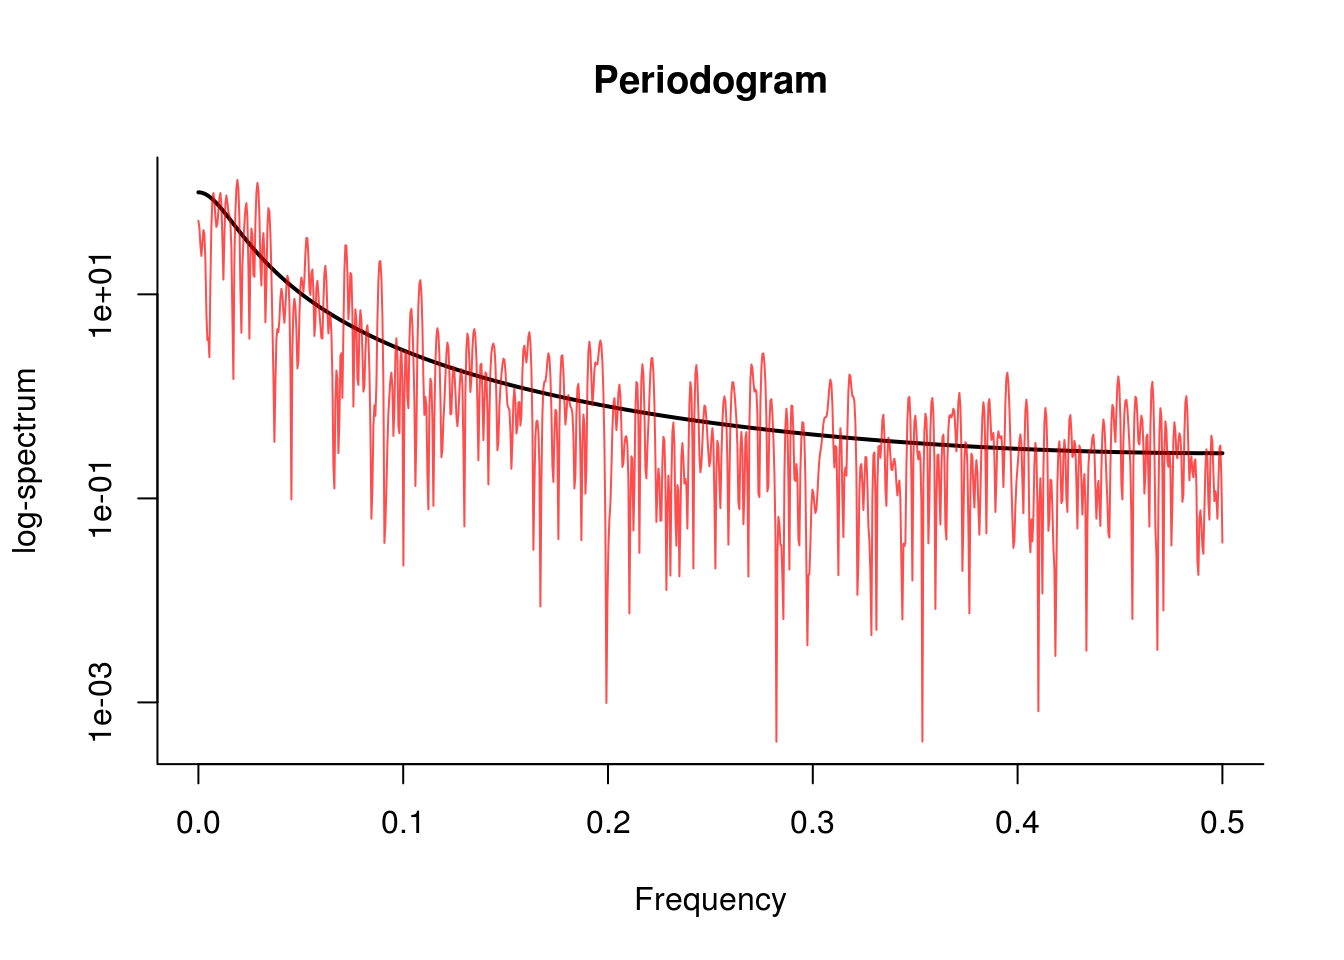
\includegraphics{timeseRies_files/figure-latex/spectrum_manually-1.pdf}

The workhorse function for spectral analysis is \texttt{spectrum}, which
computes and plots the periodogram on log scale with some default
options. Note that \texttt{spectrum} by default subtract the mean from
the series before estimating the spectral density and tapers the series
(more later). To plot the cumulative periodogram, use \texttt{cpgram}.
The latter shows the band for the Kolmogorov-Smirnov statistic. Note the
presence of the 95 \% confidence interval. The width of the center mark
on it indicates the bandwidth.

\section{Smoothing and detrending}\label{smoothing-and-detrending}

We consider detrending of a temperature dataset from the monthly mean
temperature from the Hadley center. We first download the dataset from
the web. Typically, this file can be in a repository on your computer,
or else you can provide an URL. Common formats include CSV (loaded using
\texttt{read.csv}) and txt files (loaded via \texttt{read.table}. Be
careful with the type, headers, missing values that are encoded using
e.g. \texttt{999}. Also note that \textbf{R} transforms strings into
factors by default.

\begin{Shaded}
\begin{Highlighting}[]
\NormalTok{CET <-}\StringTok{ }\KeywordTok{url}\NormalTok{(}\StringTok{"http://www.metoffice.gov.uk/hadobs/hadcet/cetml1659on.dat"}\NormalTok{)}
\KeywordTok{writeLines}\NormalTok{(}\KeywordTok{readLines}\NormalTok{(CET, }\DataTypeTok{n =} \DecValTok{10}\NormalTok{))}
\end{Highlighting}
\end{Shaded}

\begin{verbatim}
MONTHLY MEAN CENTRAL ENGLAND TEMPERATURE (DEGREES C)                                     
1659-1973 MANLEY (Q.J.R.METEOROL.SOC., 1974)                                             
1974 ON PARKER ET AL. (INT.J.CLIM., 1992)                                                
PARKER AND HORTON (INT.J.CLIM., 2005)                                                    
                                                                                         
                                                                                         
           JAN   FEB   MAR   APR   MAY   JUN   JUL   AUG   SEP   OCT   NOV   DEC     YEAR
 1659      3.0   4.0   6.0   7.0  11.0  13.0  16.0  16.0  13.0  10.0   5.0   2.0     8.87
 1660      0.0   4.0   6.0   9.0  11.0  14.0  15.0  16.0  13.0  10.0   6.0   5.0     9.10
 1661      5.0   5.0   6.0   8.0  11.0  14.0  15.0  15.0  13.0  11.0   8.0   6.0     9.78
\end{verbatim}

\begin{Shaded}
\begin{Highlighting}[]
\NormalTok{cet <-}\StringTok{ }\KeywordTok{read.table}\NormalTok{(CET, }\DataTypeTok{sep =} \StringTok{""}\NormalTok{, }\DataTypeTok{skip =} \DecValTok{6}\NormalTok{, }\DataTypeTok{header =} \OtherTok{TRUE}\NormalTok{, }\DataTypeTok{fill =} \OtherTok{TRUE}\NormalTok{, }\DataTypeTok{na.string =} \KeywordTok{c}\NormalTok{(}\OperatorTok{-}\FloatTok{99.99}\NormalTok{, }
    \OperatorTok{-}\FloatTok{99.9}\NormalTok{))}
\KeywordTok{names}\NormalTok{(cet) <-}\StringTok{ }\KeywordTok{c}\NormalTok{(month.abb, }\StringTok{"Annual"}\NormalTok{)}
\NormalTok{## remove last row of incomplete data}
\NormalTok{cet <-}\StringTok{ }\NormalTok{cet[}\OperatorTok{-}\KeywordTok{nrow}\NormalTok{(cet), }\OperatorTok{-}\KeywordTok{ncol}\NormalTok{(cet)]}
\end{Highlighting}
\end{Shaded}

Now let us investigate the dataset in a regression context. Since it is
an irregular time series, we use \texttt{zoo} rather than \texttt{ts}.

\begin{Shaded}
\begin{Highlighting}[]
\KeywordTok{library}\NormalTok{(zoo)}
\KeywordTok{library}\NormalTok{(lubridate)}
\KeywordTok{library}\NormalTok{(forecast)}
\KeywordTok{library}\NormalTok{(nlme)}
\end{Highlighting}
\end{Shaded}

\begin{Shaded}
\begin{Highlighting}[]
\CommentTok{# Convert to time series object Create a time object using `seq`, then make}
\CommentTok{# into `yearmon` The latter has the same internal representation as `ts`}
\CommentTok{# with frequency}
\NormalTok{time <-}\StringTok{ }\NormalTok{zoo}\OperatorTok{::}\KeywordTok{as.yearmon}\NormalTok{(}\KeywordTok{seq.Date}\NormalTok{(}\DataTypeTok{from =} \KeywordTok{as.Date}\NormalTok{(}\StringTok{"1659/01/01"}\NormalTok{), }\DataTypeTok{length.out =} \KeywordTok{prod}\NormalTok{(}\KeywordTok{dim}\NormalTok{(cet)), }
    \DataTypeTok{by =} \StringTok{"month"}\NormalTok{))}
\NormalTok{CET_ts <-}\StringTok{ }\NormalTok{zoo}\OperatorTok{::}\KeywordTok{zoo}\NormalTok{(}\KeywordTok{c}\NormalTok{(}\KeywordTok{t}\NormalTok{(cet)), time)}
\KeywordTok{graphics.off}\NormalTok{()}
\KeywordTok{plot}\NormalTok{(CET_ts, }\DataTypeTok{lwd =} \FloatTok{0.2}\NormalTok{, }\DataTypeTok{ylab =} \KeywordTok{expression}\NormalTok{(}\KeywordTok{Temperature}\NormalTok{(degree }\OperatorTok{*}\StringTok{ }\NormalTok{C)), }\DataTypeTok{main =} \StringTok{"Monthly mean temperature}\CharTok{\textbackslash{}n}\StringTok{ in Central England"}\NormalTok{)}
\end{Highlighting}
\end{Shaded}

Now that we have extracted the data, we are now ready to try out with
some models to explain seasonal variability as a function of covariates
rather than via differencing. If your object is of class \texttt{ts},
the function \texttt{fourier} will do the Fourier basis of order
\texttt{K} for you directly.

\begin{Shaded}
\begin{Highlighting}[]
\CommentTok{# Create Fourier basis manually}
\NormalTok{c1 <-}\StringTok{ }\KeywordTok{cos}\NormalTok{(}\DecValTok{2} \OperatorTok{*}\StringTok{ }\NormalTok{pi }\OperatorTok{*}\StringTok{ }\KeywordTok{month}\NormalTok{(CET_ts)}\OperatorTok{/}\DecValTok{12}\NormalTok{)}
\NormalTok{s1 <-}\StringTok{ }\KeywordTok{sin}\NormalTok{(}\DecValTok{2} \OperatorTok{*}\StringTok{ }\NormalTok{pi }\OperatorTok{*}\StringTok{ }\KeywordTok{month}\NormalTok{(CET_ts)}\OperatorTok{/}\DecValTok{12}\NormalTok{)}
\NormalTok{c2 <-}\StringTok{ }\KeywordTok{cos}\NormalTok{(}\DecValTok{4} \OperatorTok{*}\StringTok{ }\NormalTok{pi }\OperatorTok{*}\StringTok{ }\KeywordTok{month}\NormalTok{(CET_ts)}\OperatorTok{/}\DecValTok{12}\NormalTok{)}
\NormalTok{s2 <-}\StringTok{ }\KeywordTok{sin}\NormalTok{(}\DecValTok{4} \OperatorTok{*}\StringTok{ }\NormalTok{pi }\OperatorTok{*}\StringTok{ }\KeywordTok{month}\NormalTok{(CET_ts)}\OperatorTok{/}\DecValTok{12}\NormalTok{)}

\CommentTok{# Can also incorporate using fourier with `ts` objects.}
\NormalTok{ts1_a <-}\StringTok{ }\KeywordTok{lm}\NormalTok{(CET_ts }\OperatorTok{~}\StringTok{ }\NormalTok{time }\OperatorTok{+}\StringTok{ }\KeywordTok{fourier}\NormalTok{(CET_ts, }\DataTypeTok{K =} \DecValTok{2}\NormalTok{))}
\NormalTok{ts1_b <-}\StringTok{ }\KeywordTok{lm}\NormalTok{(CET_ts }\OperatorTok{~}\StringTok{ }\KeywordTok{seq.int}\NormalTok{(}\DecValTok{1}\NormalTok{, }\KeywordTok{length}\NormalTok{(CET_ts)) }\OperatorTok{+}\StringTok{ }\NormalTok{c1 }\OperatorTok{+}\StringTok{ }\NormalTok{s1 }\OperatorTok{+}\StringTok{ }\NormalTok{c2 }\OperatorTok{+}\StringTok{ }\NormalTok{s2)}
\CommentTok{# Same fitted values, different regressors for the trend - see the design}
\CommentTok{# matrix head(ts1_a$model)}
\NormalTok{forecast}\OperatorTok{::}\KeywordTok{Acf}\NormalTok{(}\KeywordTok{resid}\NormalTok{(ts1_a), }\DataTypeTok{main =} \StringTok{"Correlogram of residuals"}\NormalTok{)}
\end{Highlighting}
\end{Shaded}

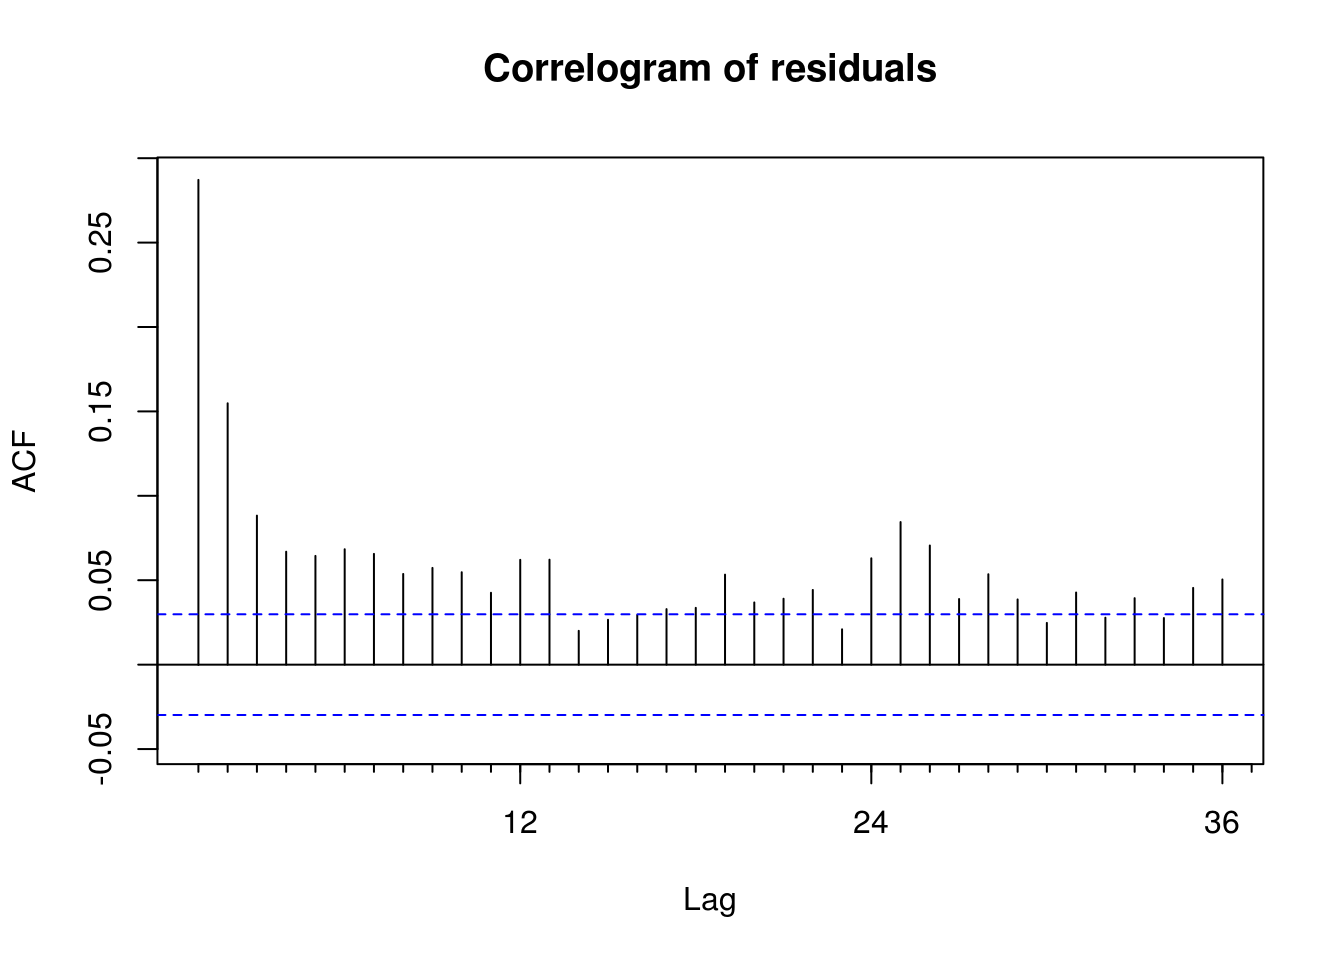
\includegraphics{timeseRies_files/figure-latex/reg_fourier-1.pdf}

\begin{Shaded}
\begin{Highlighting}[]
\NormalTok{forecast}\OperatorTok{::}\KeywordTok{Pacf}\NormalTok{(}\KeywordTok{resid}\NormalTok{(ts1_b), }\DataTypeTok{main =} \StringTok{"Partial correlogram of residuals"}\NormalTok{)}
\end{Highlighting}
\end{Shaded}

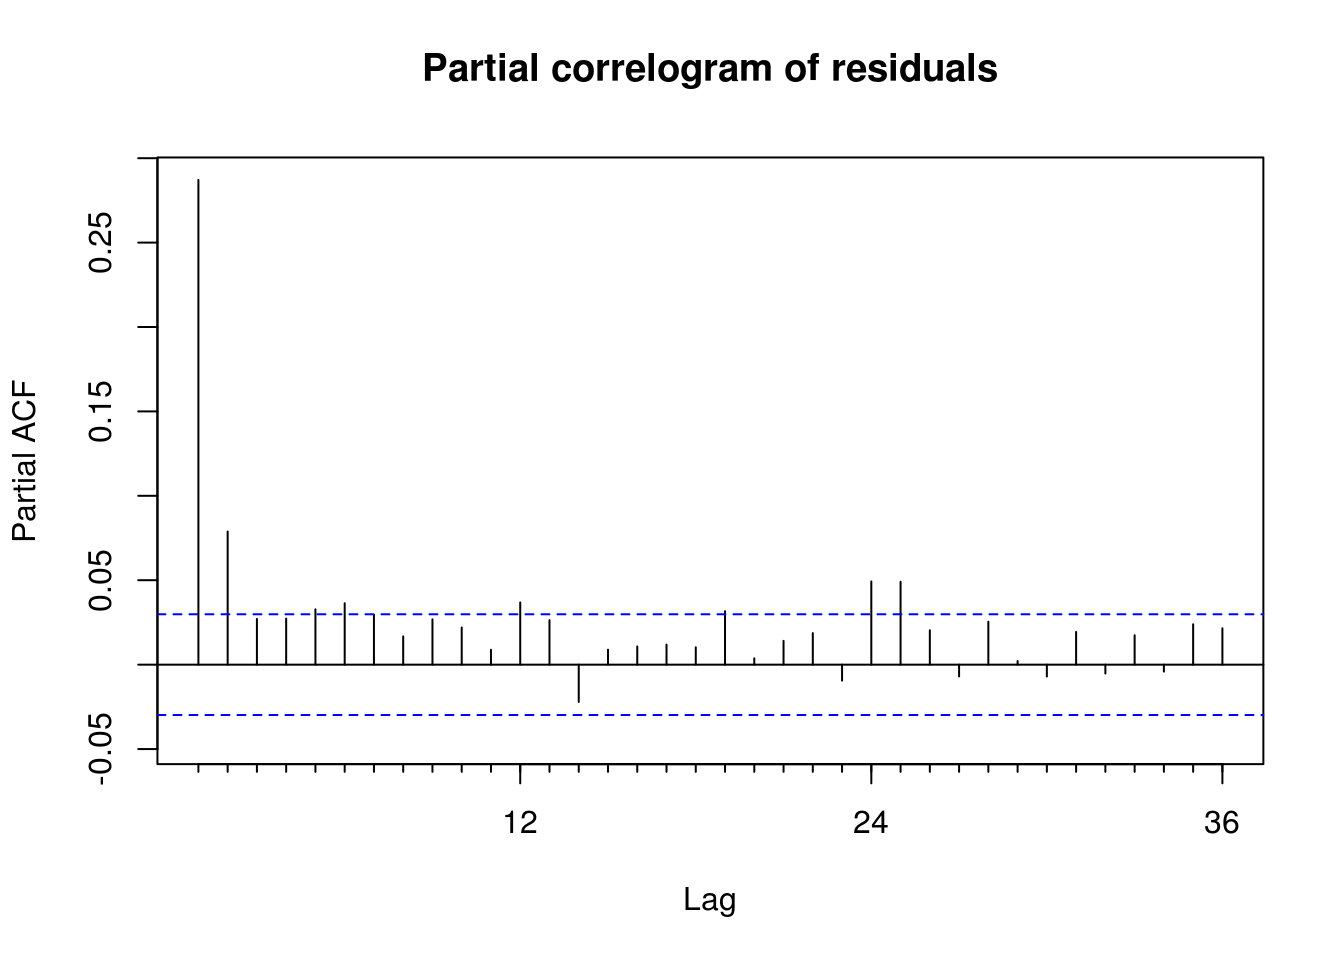
\includegraphics{timeseRies_files/figure-latex/reg_fourier-2.pdf}

One could also replace the Fourier terms with seasonal dummies (possibly
removing the intercept if 12 dummies are set). However, the use of
Fourier terms, where appropriate, allows for more parsimonious
modelling. Always keep pairs of sine and cosine together.

The function \texttt{stl} decomposes a time series into seasonal trend
and irregular components. We illustrate the use of the function on the
\texttt{deaths} dataset.

\begin{Shaded}
\begin{Highlighting}[]
\NormalTok{seasonal_decomp_death <-}\StringTok{ }\KeywordTok{stl}\NormalTok{(deaths, }\DataTypeTok{s.window =} \StringTok{"periodic"}\NormalTok{)}
\KeywordTok{plot}\NormalTok{(seasonal_decomp_death)}
\end{Highlighting}
\end{Shaded}

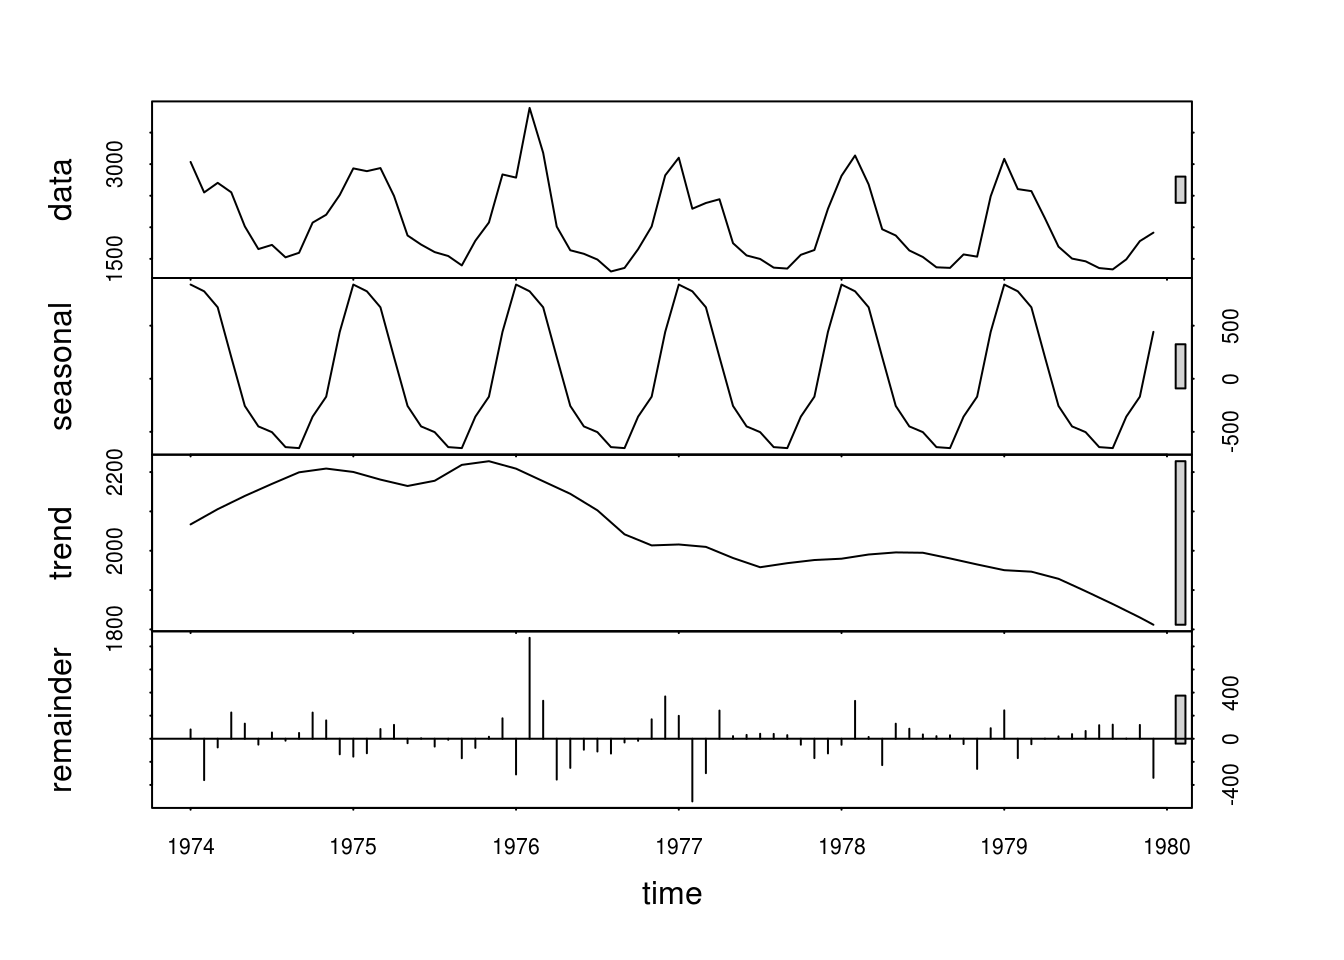
\includegraphics{timeseRies_files/figure-latex/unnamed-chunk-8-1.pdf}

\subsection{\texorpdfstring{Exercise 4: Mauna Loa Atmospheric
CO\textsubscript{2}
Concentration}{Exercise 4: Mauna Loa Atmospheric CO2 Concentration}}\label{exercise-4-mauna-loa-atmospheric-co2-concentration}

\begin{enumerate}
\def\labelenumi{\arabic{enumi}.}
\tightlist
\item
  Load and plot the CO\textsubscript{2} dataset from
  \href{ftp://aftp.cmdl.noaa.gov/products/trends/co2/co2_mm_mlo.txt}{NOAA}.
  Pay special attention to the format, missing values, the handling of
  string and the description. Use \texttt{?read.table} for help, and
  look carefully at arguments \texttt{file}, \texttt{sep},
  \texttt{na.strings}, \texttt{skip} and \texttt{stringsAsFactors}. From
  now on, we will work with the complete series (termed interpolated in
  the description).
\item
  Try removing the trend using a linear model. Plot the residuals
  against month of the year.
\item
  Remove the trend and the periodicity with a Fourier basis (with period
  12). Be sure to include both \texttt{sin} and \texttt{cos} terms
  together. Recall that the standard Wald tests for the coefficients is
  not valid in the presence of autocorrelation! You could also use
  \texttt{poly} or \texttt{splines::bs} to fit polynomials or splines to
  your series.
\item
  Plot the lagged residuals. Are there evidence of correlation?
\item
  Use the function \texttt{filter} to smooth the series using a 12
  period moving average.
\item
  Inspect the spectrum of the raw series and of the smoothed version.
\item
  Inspect the spectrum of the detrended raw series.
\item
  Test for stationarity of the deseasonalized and detrended residuals
  using the KPSS test viz. \texttt{tseries::kpss.test}.
\item
  Use the \texttt{decompose} and the \texttt{stl} functions to obtain
  residuals.
\item
  Plot the (partial) correlogram for both decomposition and compare them
  with the output of the linear model.
\end{enumerate}

\section{Solutions to Exercises}\label{solutions-to-exercises}

\subsection{Solutions 1: Beaver
temperature}\label{solutions-1-beaver-temperature}

\begin{enumerate}
\def\labelenumi{\arabic{enumi}.}
\tightlist
\item
  Load the \texttt{beav2} data from the library \texttt{MASS}.
\item
  Examine the data frame using \texttt{summary}, \texttt{head},
  \texttt{tail}. Query the help with \texttt{?beav2} for a description
  of the dataset
\item
  Transform the temperature data into a time series object and plot the
  latter.
\item
  Fit a linear model using \texttt{lm} and the variable \texttt{activ}
  as factor, viz.
  \texttt{lin\_mod\ \textless{}-\ lm(temp\textasciitilde{}as.factor(activ),\ data=beav2)}.
  Overlay the means on your plot with \texttt{lines(fitted(lin\_mod))}
  replacing \texttt{lin\_mod} with your \texttt{lm} result.
\item
  Inspect the residuals (\texttt{resid(lin\_mod)}) and determine whether
  there is any evidence of trend or seasonality.
\item
  Look at a quantile-quantile (Q-Q) plot to assess normality. You can
  use the command \texttt{qqnorm} if you don't want to transform
  manually the residuals with \texttt{qqline} or use
  \texttt{plot(lin\_mod,\ which=2)}.
\item
  Plot the lag-one residuals at time \(t\) and \(t-1\). Is the
  dependence approximately linear?
\end{enumerate}

\begin{Shaded}
\begin{Highlighting}[]
\KeywordTok{data}\NormalTok{(beav2, }\DataTypeTok{package =} \StringTok{"MASS"}\NormalTok{)}
\StringTok{`}\DataTypeTok{?}\StringTok{`}\NormalTok{(MASS}\OperatorTok{::}\NormalTok{beav2)}
\NormalTok{beav2}\OperatorTok{$}\NormalTok{hours <-}\StringTok{ }\KeywordTok{with}\NormalTok{(beav2, }\DecValTok{24} \OperatorTok{*}\StringTok{ }\NormalTok{(day }\OperatorTok{-}\StringTok{ }\DecValTok{307}\NormalTok{) }\OperatorTok{+}\StringTok{ }\KeywordTok{trunc}\NormalTok{(time}\OperatorTok{/}\DecValTok{100}\NormalTok{) }\OperatorTok{+}\StringTok{ }\NormalTok{(time}\OperatorTok\DecValTok{100}\NormalTok{)}\OperatorTok{/}\DecValTok{60}\NormalTok{)}
\KeywordTok{summary}\NormalTok{(beav2)}
\end{Highlighting}
\end{Shaded}

\begin{verbatim}
      day             time           temp           activ     
 Min.   :307.0   Min.   :   0   Min.   :36.58   Min.   :0.00  
 1st Qu.:307.0   1st Qu.:1128   1st Qu.:37.15   1st Qu.:0.00  
 Median :307.0   Median :1535   Median :37.73   Median :1.00  
 Mean   :307.1   Mean   :1446   Mean   :37.60   Mean   :0.62  
 3rd Qu.:307.0   3rd Qu.:1942   3rd Qu.:37.98   3rd Qu.:1.00  
 Max.   :308.0   Max.   :2350   Max.   :38.35   Max.   :1.00  
     hours      
 Min.   : 9.50  
 1st Qu.:13.62  
 Median :17.75  
 Mean   :17.75  
 3rd Qu.:21.88  
 Max.   :26.00  
\end{verbatim}

\begin{Shaded}
\begin{Highlighting}[]
\KeywordTok{head}\NormalTok{(beav2)}
\end{Highlighting}
\end{Shaded}

\begin{verbatim}
  day time  temp activ     hours
1 307  930 36.58     0  9.500000
2 307  940 36.73     0  9.666667
3 307  950 36.93     0  9.833333
4 307 1000 37.15     0 10.000000
5 307 1010 37.23     0 10.166667
6 307 1020 37.24     0 10.333333
\end{verbatim}

\begin{Shaded}
\begin{Highlighting}[]
\KeywordTok{tail}\NormalTok{(beav2)}
\end{Highlighting}
\end{Shaded}

\begin{verbatim}
    day time  temp activ    hours
95  308  110 37.76     1 25.16667
96  308  120 37.73     1 25.33333
97  308  130 37.77     1 25.50000
98  308  140 38.01     1 25.66667
99  308  150 38.04     1 25.83333
100 308  200 38.07     1 26.00000
\end{verbatim}

\begin{Shaded}
\begin{Highlighting}[]
\CommentTok{# Fancy time series object}
\NormalTok{hours <-}\StringTok{ }\KeywordTok{seq}\NormalTok{(}\KeywordTok{ISOdatetime}\NormalTok{(}\DecValTok{1990}\NormalTok{, }\DecValTok{11}\NormalTok{, }\DecValTok{3}\NormalTok{, }\DecValTok{9}\NormalTok{, }\DecValTok{30}\NormalTok{, }\DecValTok{0}\NormalTok{), }\KeywordTok{ISOdatetime}\NormalTok{(}\DecValTok{1990}\NormalTok{, }\DecValTok{11}\NormalTok{, }\DecValTok{4}\NormalTok{, }\DecValTok{2}\NormalTok{, }
    \DecValTok{0}\NormalTok{, }\DecValTok{0}\NormalTok{), }\DataTypeTok{by =}\NormalTok{ (}\DecValTok{60} \OperatorTok{*}\StringTok{ }\DecValTok{10}\NormalTok{))}
\KeywordTok{plot}\NormalTok{(xts}\OperatorTok{::}\KeywordTok{xts}\NormalTok{(beav2[, }\StringTok{"temp"}\NormalTok{], hours), }\DataTypeTok{main =} \StringTok{"Body temperature of beaver"}\NormalTok{, }
    \DataTypeTok{ylab =} \StringTok{"Temperature (in degree Celcius)"}\NormalTok{)}
\end{Highlighting}
\end{Shaded}

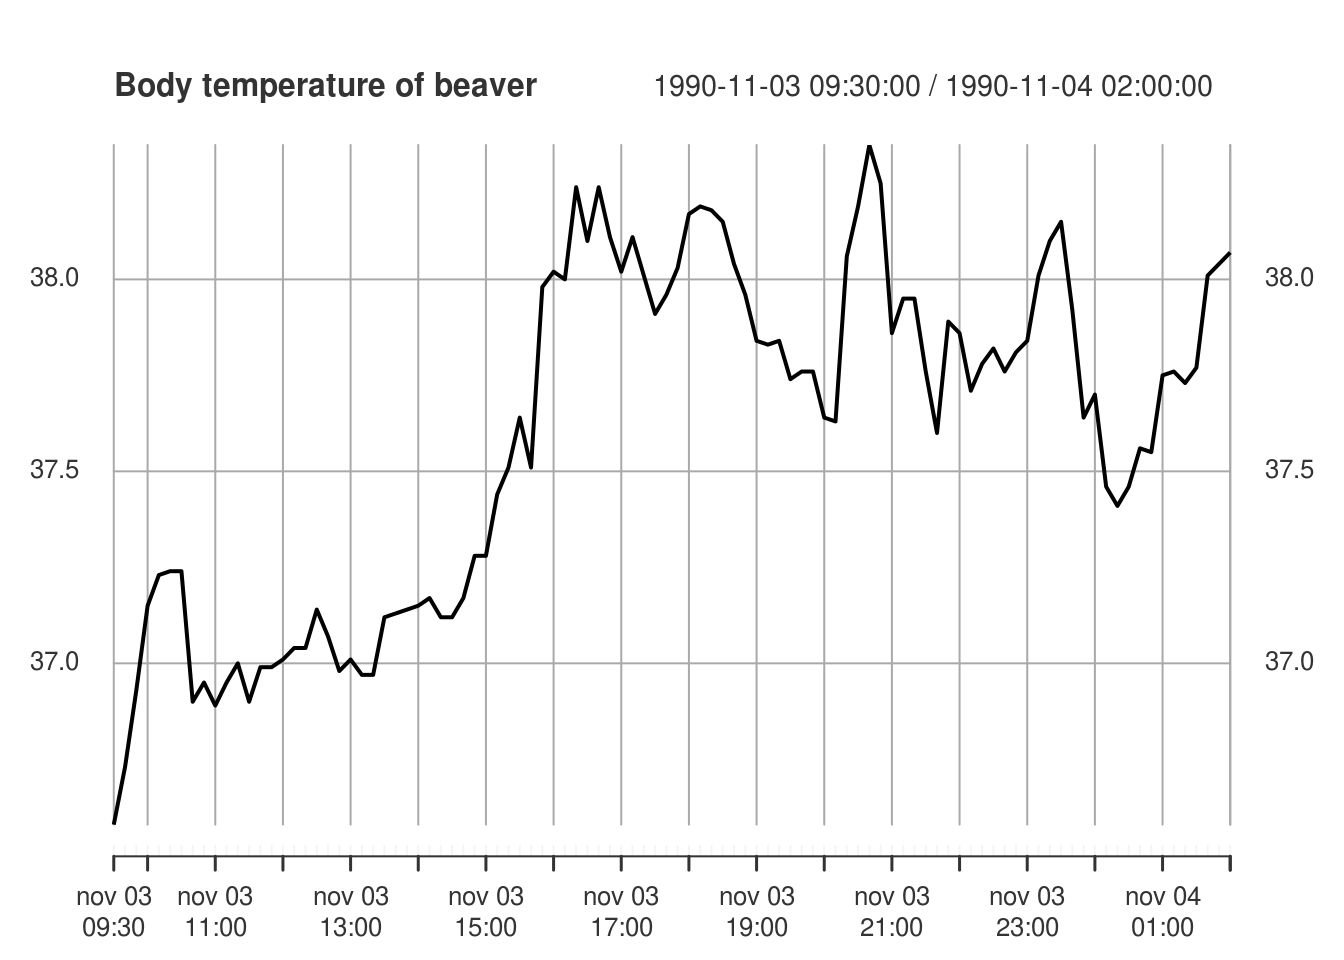
\includegraphics{timeseRies_files/figure-latex/Question_1-1.pdf}

\begin{Shaded}
\begin{Highlighting}[]
\CommentTok{# Vanilla ts - works ok for regular time series}
\NormalTok{temp <-}\StringTok{ }\KeywordTok{ts}\NormalTok{(beav2[, }\StringTok{"temp"}\NormalTok{], }\DataTypeTok{start =} \FloatTok{9.5}\NormalTok{, }\DataTypeTok{frequency =} \DecValTok{6}\NormalTok{)}
\KeywordTok{plot}\NormalTok{(temp, }\DataTypeTok{main =} \StringTok{"Body temperature of beaver"}\NormalTok{, }\DataTypeTok{ylab =} \StringTok{"Temperature (in degree Celcius)"}\NormalTok{)}
\NormalTok{lin_mod <-}\StringTok{ }\KeywordTok{lm}\NormalTok{(temp }\OperatorTok{~}\StringTok{ }\KeywordTok{as.factor}\NormalTok{(activ), }\DataTypeTok{data =}\NormalTok{ beav2)}
\KeywordTok{lines}\NormalTok{(beav2[, }\StringTok{"hours"}\NormalTok{], }\KeywordTok{fitted}\NormalTok{(lin_mod), }\DataTypeTok{col =} \StringTok{"blue"}\NormalTok{)}
\end{Highlighting}
\end{Shaded}

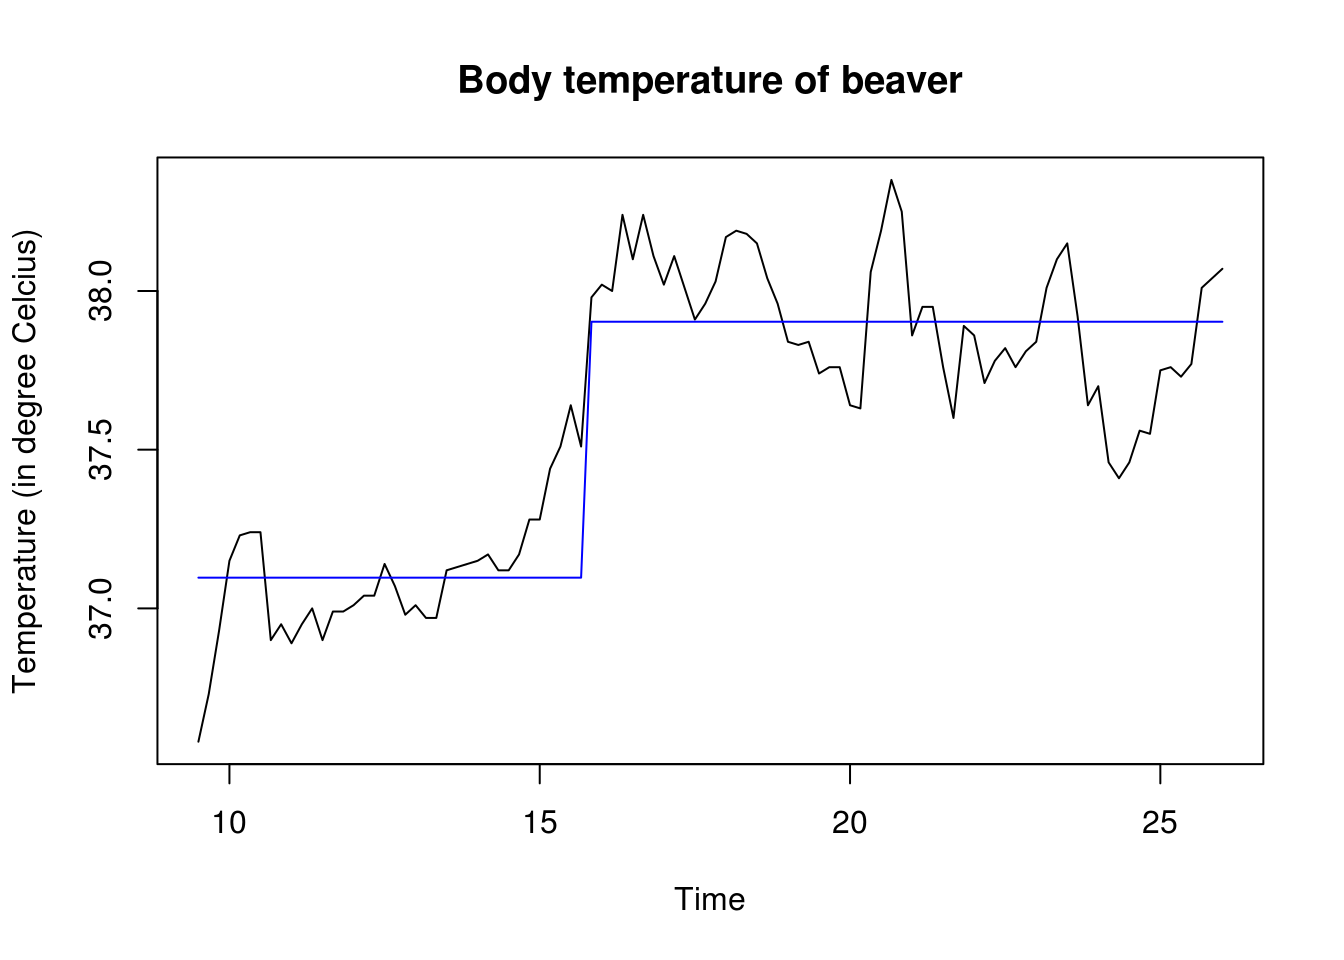
\includegraphics{timeseRies_files/figure-latex/Question_1-2.pdf}

\begin{Shaded}
\begin{Highlighting}[]
\CommentTok{# Some trend remaining in the first part, before time}
\end{Highlighting}
\end{Shaded}

\begin{Shaded}
\begin{Highlighting}[]
\KeywordTok{plot}\NormalTok{(}\KeywordTok{residuals}\NormalTok{(lin_mod), }\DataTypeTok{ylab =} \StringTok{"Residuals"}\NormalTok{, }\DataTypeTok{main =} \StringTok{"Residuals of linear model with simple change-point"}\NormalTok{)}
\KeywordTok{abline}\NormalTok{(}\DataTypeTok{h =} \DecValTok{0}\NormalTok{)}
\end{Highlighting}
\end{Shaded}

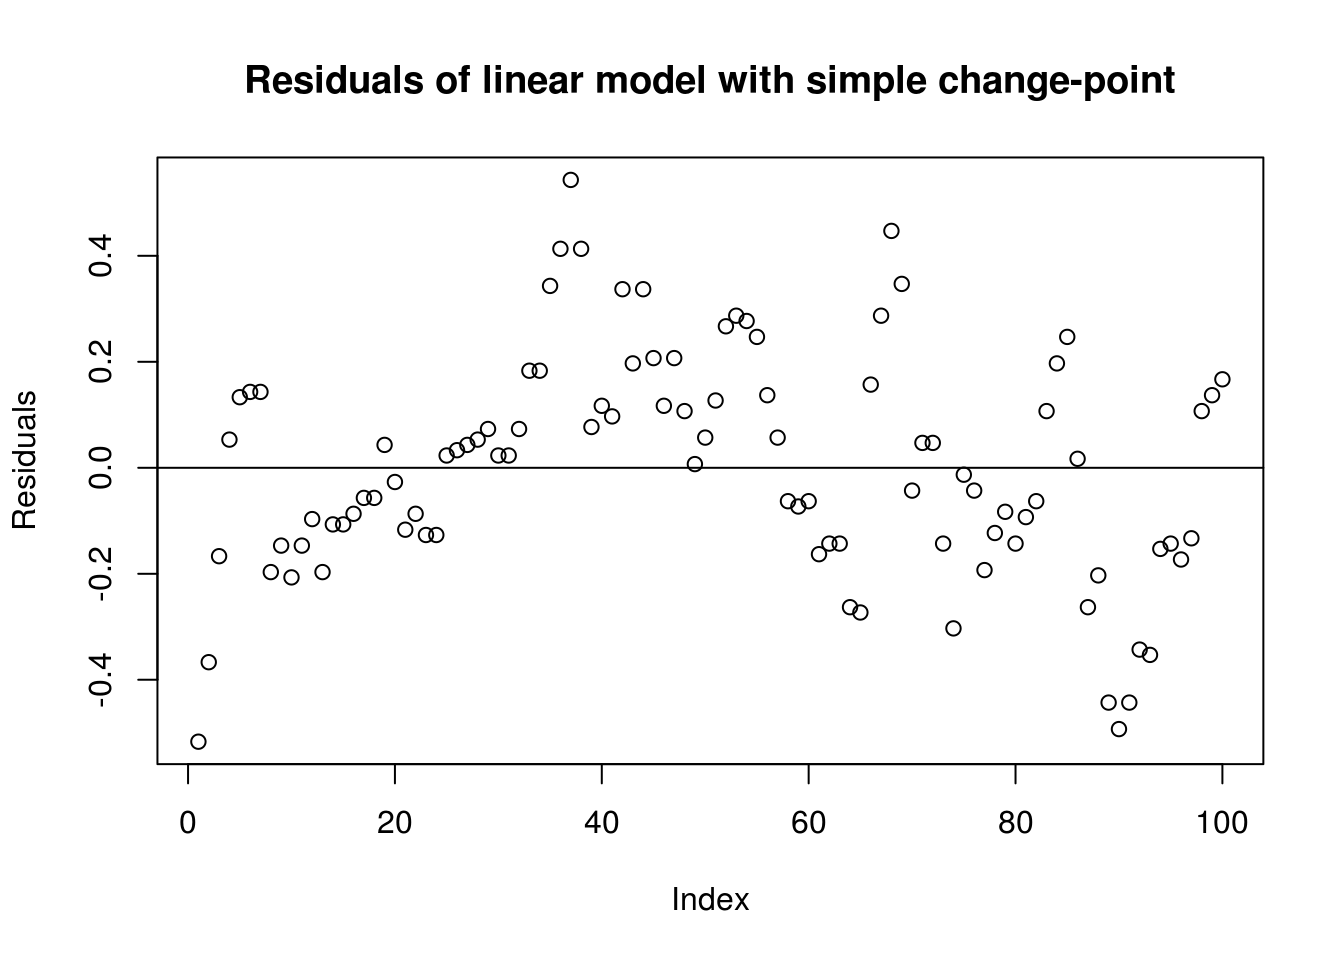
\includegraphics{timeseRies_files/figure-latex/unnamed-chunk-9-1.pdf}

\begin{Shaded}
\begin{Highlighting}[]
\CommentTok{# Q-Q plot (1) with output from lm}
\KeywordTok{plot}\NormalTok{(lin_mod, }\DataTypeTok{which =} \DecValTok{2}\NormalTok{)}
\end{Highlighting}
\end{Shaded}

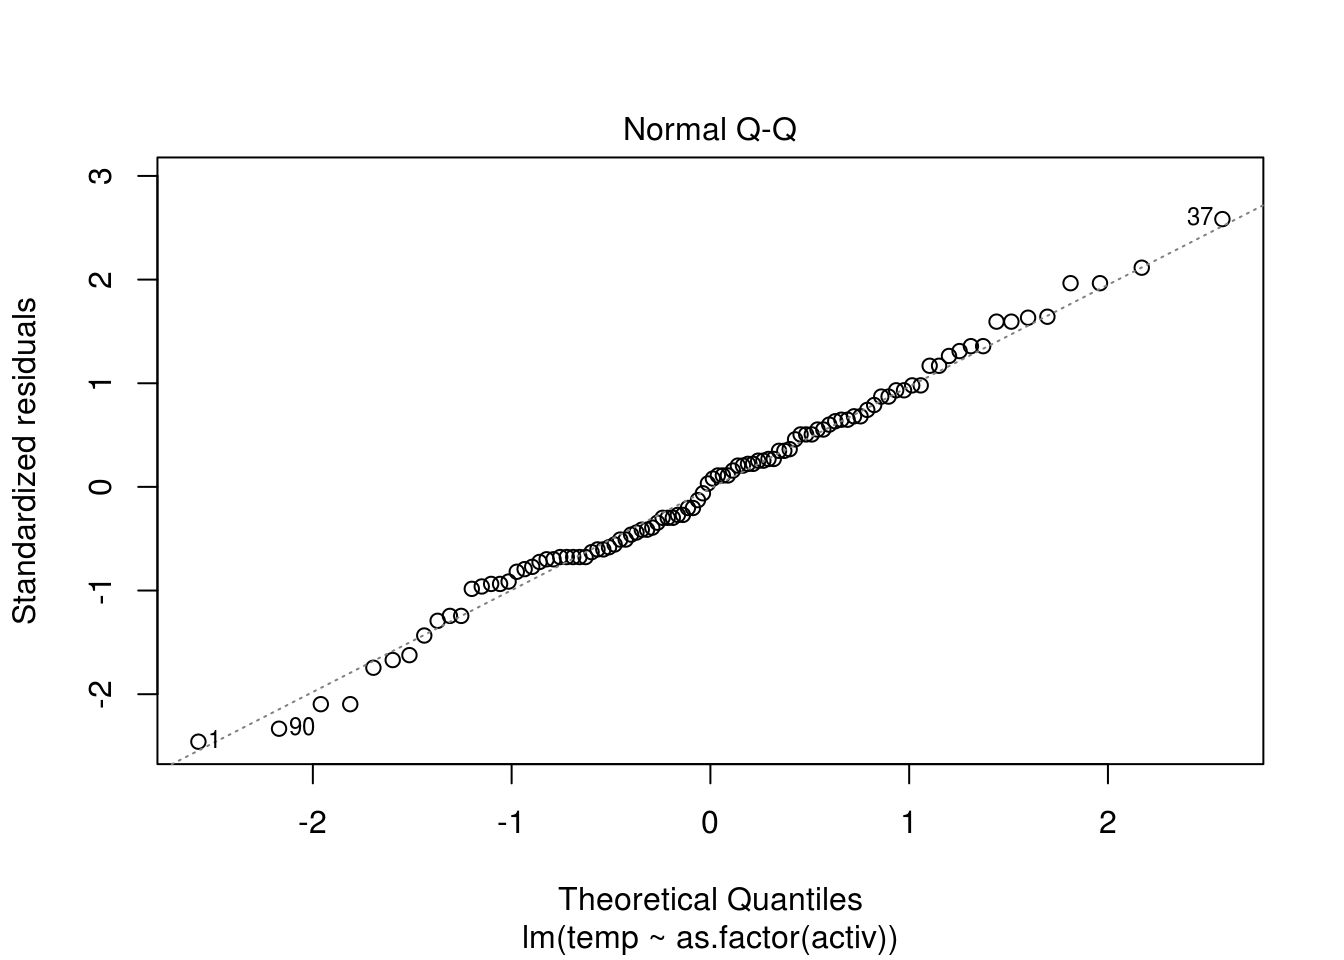
\includegraphics{timeseRies_files/figure-latex/unnamed-chunk-9-2.pdf}

\begin{Shaded}
\begin{Highlighting}[]
\CommentTok{# (2) with qqnorm and tentative line with quartiles}
\KeywordTok{qqnorm}\NormalTok{(}\KeywordTok{residuals}\NormalTok{(lin_mod))}
\KeywordTok{qqline}\NormalTok{(}\KeywordTok{residuals}\NormalTok{(lin_mod))}
\end{Highlighting}
\end{Shaded}

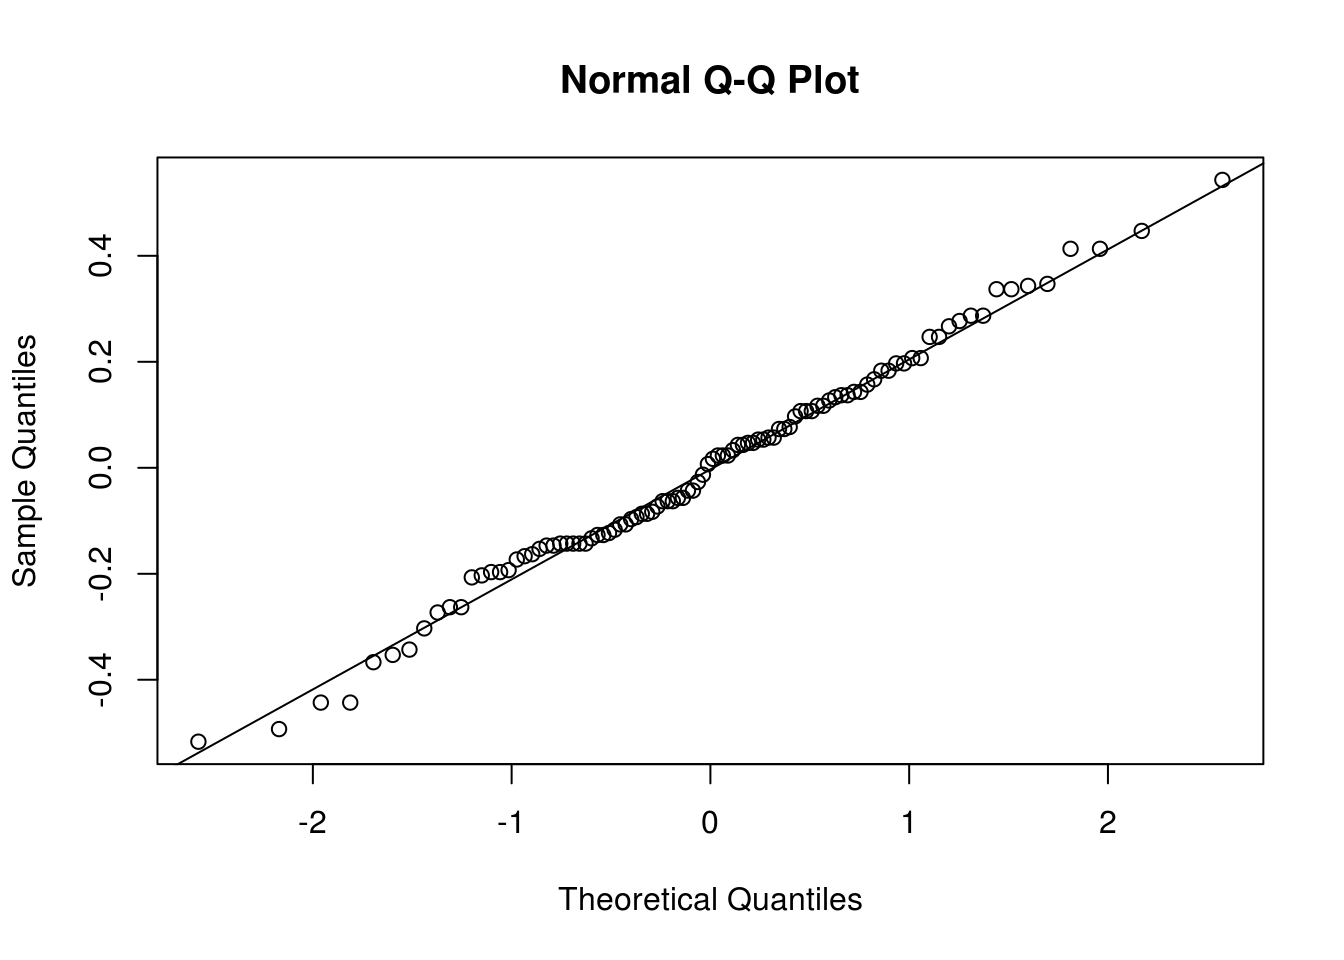
\includegraphics{timeseRies_files/figure-latex/unnamed-chunk-9-3.pdf}

\begin{Shaded}
\begin{Highlighting}[]
\CommentTok{# (3) standardized manually}
\NormalTok{res <-}\StringTok{ }\KeywordTok{residuals}\NormalTok{(lin_mod)}
\KeywordTok{plot}\NormalTok{(}\KeywordTok{qnorm}\NormalTok{(}\KeywordTok{rank}\NormalTok{(res)}\OperatorTok{/}\NormalTok{(}\KeywordTok{length}\NormalTok{(res) }\OperatorTok{+}\StringTok{ }\DecValTok{1}\NormalTok{)), res}\OperatorTok{/}\KeywordTok{sd}\NormalTok{(res), }\DataTypeTok{pty =} \StringTok{"s"}\NormalTok{, }\DataTypeTok{bty =} \StringTok{"l"}\NormalTok{, }
    \DataTypeTok{xlab =} \StringTok{"Theoretical Quantiles"}\NormalTok{, }\DataTypeTok{ylab =} \StringTok{"Sample Quantiles"}\NormalTok{, }\DataTypeTok{main =} \StringTok{"Normal Q-Q plot"}\NormalTok{, }
    \DataTypeTok{pch =} \DecValTok{20}\NormalTok{, }\DataTypeTok{col =} \KeywordTok{rgb}\NormalTok{(}\DecValTok{0}\NormalTok{, }\DecValTok{0}\NormalTok{, }\DecValTok{0}\NormalTok{, }\FloatTok{0.5}\NormalTok{))}
\KeywordTok{abline}\NormalTok{(}\DataTypeTok{a =} \DecValTok{0}\NormalTok{, }\DataTypeTok{b =} \DecValTok{1}\NormalTok{)}
\end{Highlighting}
\end{Shaded}

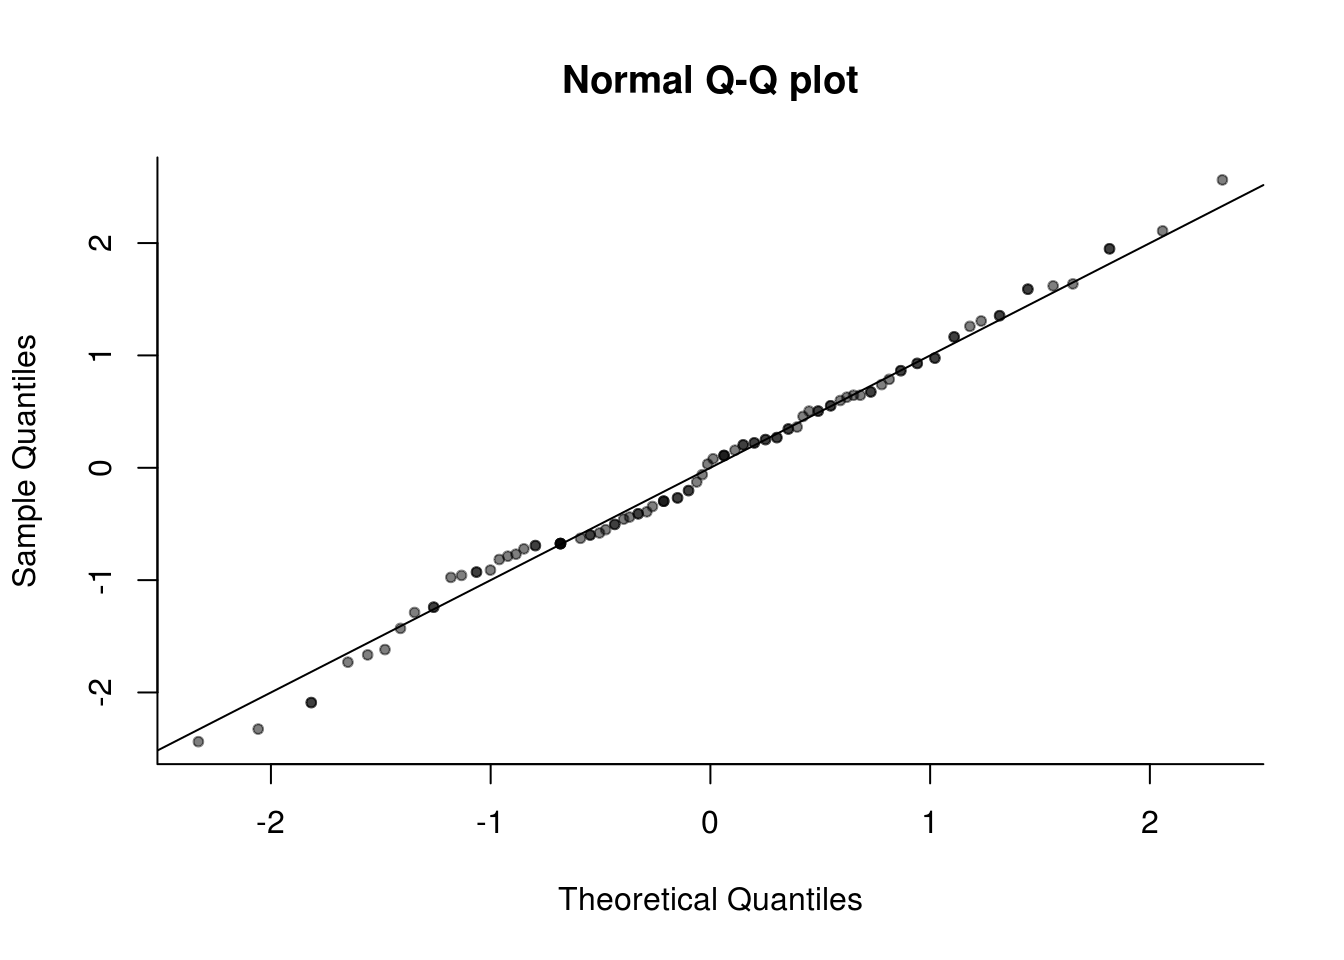
\includegraphics{timeseRies_files/figure-latex/unnamed-chunk-9-4.pdf}

\begin{Shaded}
\begin{Highlighting}[]
\KeywordTok{plot}\NormalTok{(res[}\OperatorTok{-}\KeywordTok{length}\NormalTok{(res)], res[}\OperatorTok{-}\DecValTok{1}\NormalTok{], }\DataTypeTok{xlab =} \KeywordTok{expression}\NormalTok{(Y[t }\OperatorTok{-}\StringTok{ }\DecValTok{1}\NormalTok{]), }\DataTypeTok{ylab =} \KeywordTok{expression}\NormalTok{(Y[t]), }
    \DataTypeTok{main =} \StringTok{"Lagged residuals"}\NormalTok{)}
\end{Highlighting}
\end{Shaded}

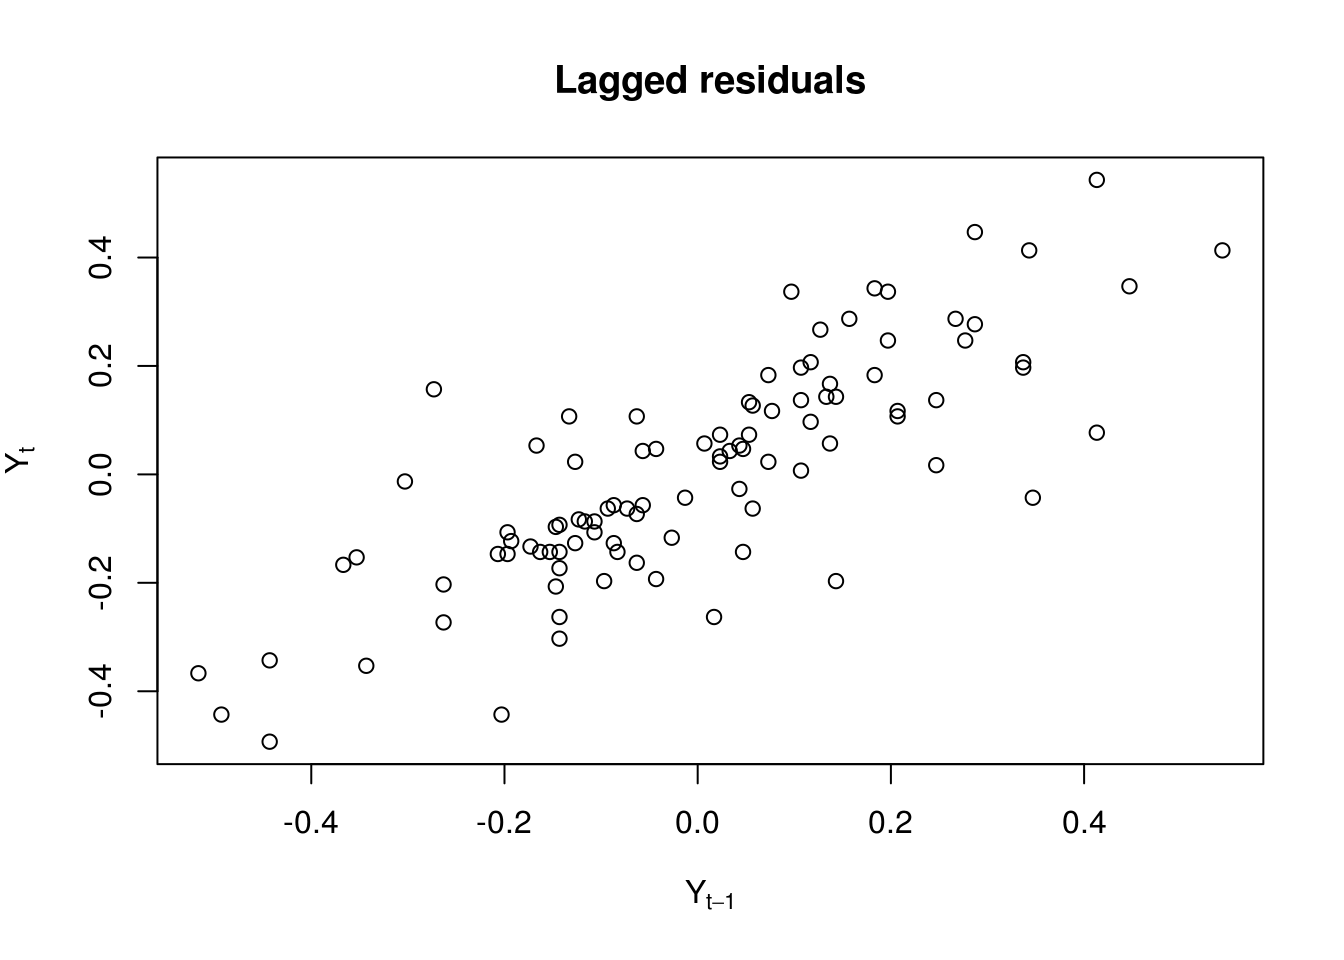
\includegraphics{timeseRies_files/figure-latex/unnamed-chunk-9-5.pdf}

\subsection{Solutions 2: SP500 daily
returns}\label{solutions-2-sp500-daily-returns}

\begin{enumerate}
\def\labelenumi{\arabic{enumi}.}
\tightlist
\item
  Download the dataset using the following command
\item
  Obtain the daily percent return series and plot the latter against
  time.
\item
  With the help of graphs, discuss evidences of seasonality and
  nonstationarity. Are there seasons of returns?
\item
  Plot the (partial) correlogram of both the raw and the return series.
  Try the acf with \texttt{na.action=na.pass} and without (by
  e.g.~converting the series to a vector using \texttt{as.vector}.
  Comment on the impact of ignoring time stamps.
\item
  Plot the (partial) correlogram of the absolute value of the return
  series and of the squared return series. What do you see?
\end{enumerate}

\begin{Shaded}
\begin{Highlighting}[]
\NormalTok{sp500 <-}\StringTok{ }\NormalTok{tseries}\OperatorTok{::}\KeywordTok{get.hist.quote}\NormalTok{(}\DataTypeTok{instrument =} \StringTok{"^GSPC"}\NormalTok{, }\DataTypeTok{start =} \StringTok{"2000-01-01"}\NormalTok{, }
    \DataTypeTok{end =} \StringTok{"2016-12-31"}\NormalTok{, }\DataTypeTok{quote =} \StringTok{"AdjClose"}\NormalTok{, }\DataTypeTok{provider =} \StringTok{"yahoo"}\NormalTok{, }\DataTypeTok{origin =} \StringTok{"1970-01-01"}\NormalTok{, }
    \DataTypeTok{compression =} \StringTok{"d"}\NormalTok{, }\DataTypeTok{retclass =} \StringTok{"zoo"}\NormalTok{)}
\end{Highlighting}
\end{Shaded}

\begin{verbatim}
time series starts 2000-01-03
time series ends   2016-12-30
\end{verbatim}

\begin{Shaded}
\begin{Highlighting}[]
\KeywordTok{library}\NormalTok{(xts)}
\KeywordTok{library}\NormalTok{(lubridate)}
\CommentTok{# Daily return in percentage}
\NormalTok{spret <-}\StringTok{ }\DecValTok{100} \OperatorTok{*}\StringTok{ }\KeywordTok{diff}\NormalTok{(}\KeywordTok{log}\NormalTok{(sp500))}
\KeywordTok{plot}\NormalTok{(spret, }\DataTypeTok{ylab =} \StringTok{"Daily returns (%)"}\NormalTok{, }\DataTypeTok{main =} \StringTok{"Percentage daily returns of the SP-500"}\NormalTok{)}
\CommentTok{# local trend to see if there is any evidence of non-zero trend}
\KeywordTok{lines}\NormalTok{(}\KeywordTok{index}\NormalTok{(spret), }\KeywordTok{lowess}\NormalTok{(spret, }\DataTypeTok{f =} \DecValTok{1}\OperatorTok{/}\DecValTok{5}\NormalTok{)}\OperatorTok{$}\NormalTok{y, }\DataTypeTok{col =} \DecValTok{2}\NormalTok{, }\DataTypeTok{lwd =} \DecValTok{2}\NormalTok{)}
\end{Highlighting}
\end{Shaded}

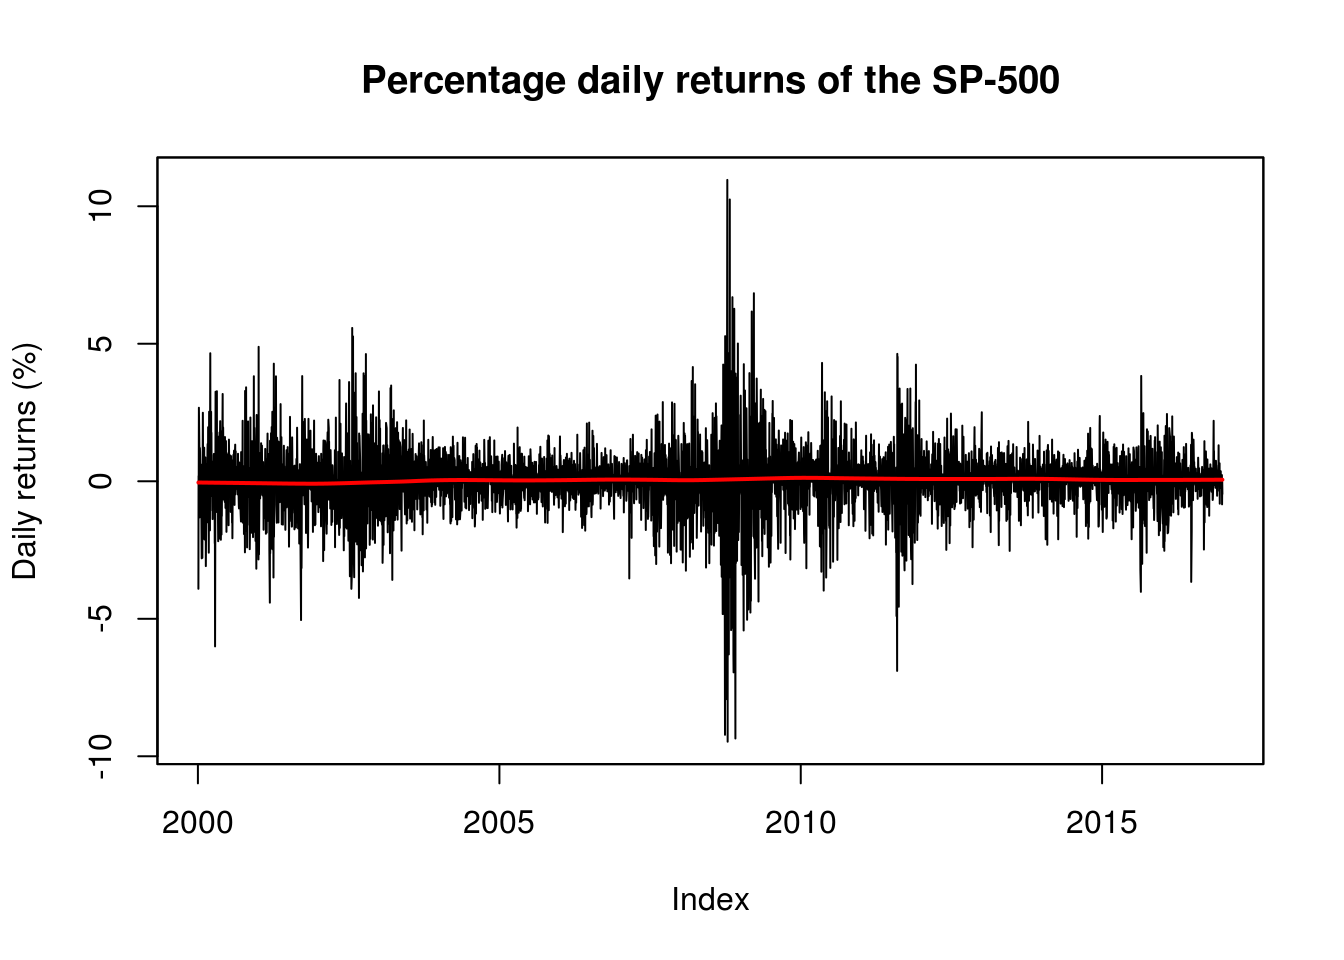
\includegraphics{timeseRies_files/figure-latex/Question_2-1.pdf}

\begin{Shaded}
\begin{Highlighting}[]
\CommentTok{# Volatility as function of month}
\KeywordTok{plot}\NormalTok{(}\KeywordTok{jitter}\NormalTok{(}\KeywordTok{month}\NormalTok{(spret), }\DataTypeTok{amount =} \DecValTok{1}\OperatorTok{/}\DecValTok{3}\NormalTok{), spret, }\DataTypeTok{pch =} \DecValTok{20}\NormalTok{, }\DataTypeTok{ylab =} \StringTok{"Daily percent returns"}\NormalTok{, }
    \DataTypeTok{xlab =} \StringTok{"Month"}\NormalTok{, }\DataTypeTok{bty =} \StringTok{"l"}\NormalTok{)}
\end{Highlighting}
\end{Shaded}

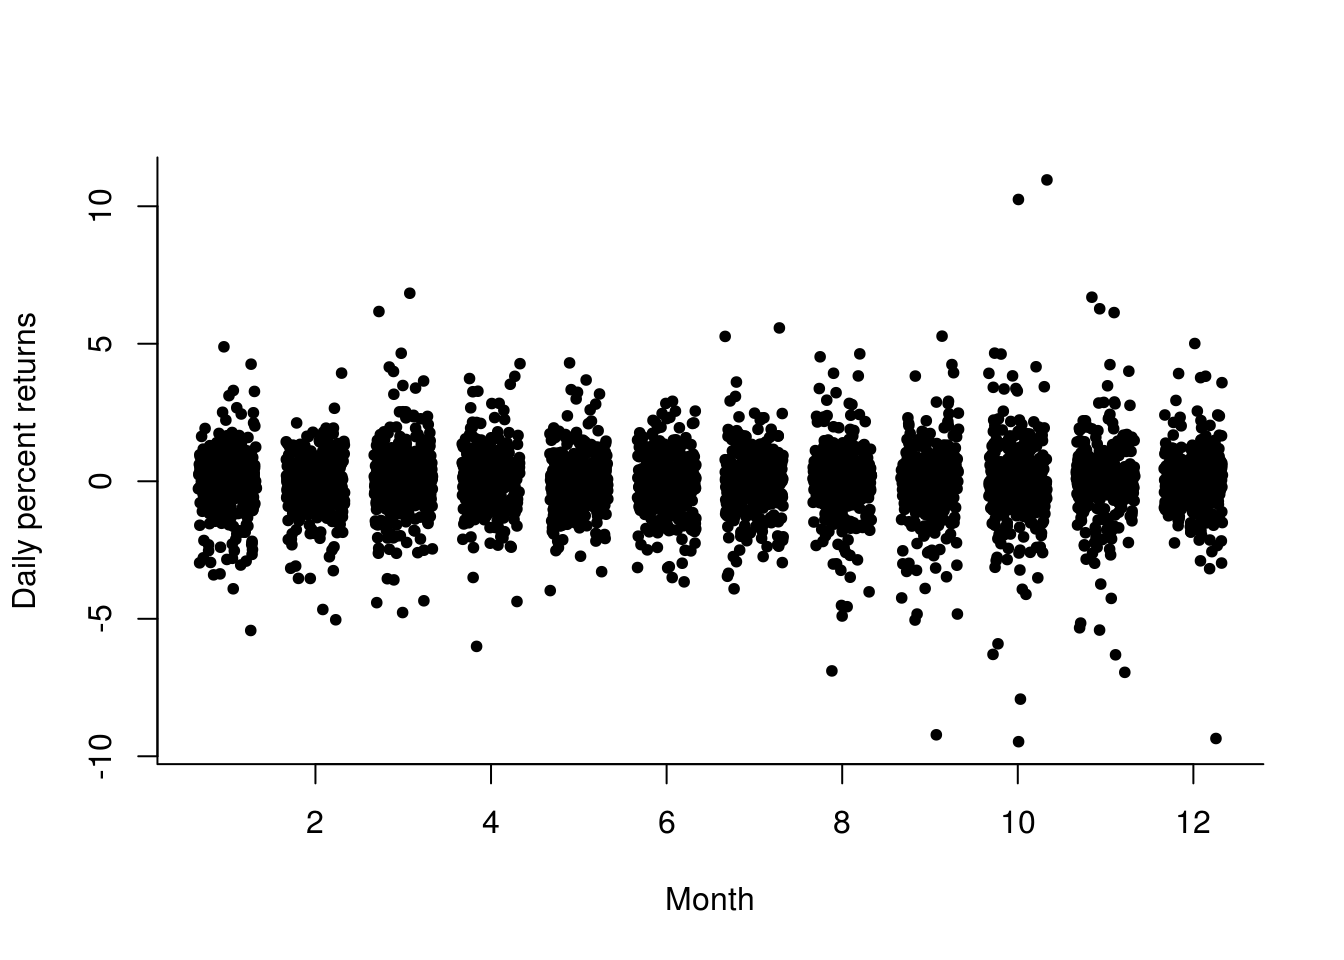
\includegraphics{timeseRies_files/figure-latex/Question_2-2.pdf}

\begin{Shaded}
\begin{Highlighting}[]
\KeywordTok{boxplot}\NormalTok{(}\KeywordTok{as.vector}\NormalTok{(spret) }\OperatorTok{~}\StringTok{ }\KeywordTok{factor}\NormalTok{(}\KeywordTok{wday}\NormalTok{(spret), }\DataTypeTok{labels =} \KeywordTok{c}\NormalTok{(}\StringTok{"Mon"}\NormalTok{, }\StringTok{"Tue"}\NormalTok{, }\StringTok{"Wed"}\NormalTok{, }
    \StringTok{"Thu"}\NormalTok{, }\StringTok{"Fri"}\NormalTok{)), }\DataTypeTok{xlab =} \StringTok{"Day of the week"}\NormalTok{, }\DataTypeTok{pch =} \DecValTok{20}\NormalTok{, }\DataTypeTok{col =} \KeywordTok{rgb}\NormalTok{(}\DecValTok{0}\NormalTok{, }\DecValTok{0}\NormalTok{, }\DecValTok{0}\NormalTok{, }\FloatTok{0.4}\NormalTok{), }
    \DataTypeTok{ylab =} \StringTok{"Daily percent returns"}\NormalTok{, }\DataTypeTok{bty =} \StringTok{"l"}\NormalTok{)}
\end{Highlighting}
\end{Shaded}

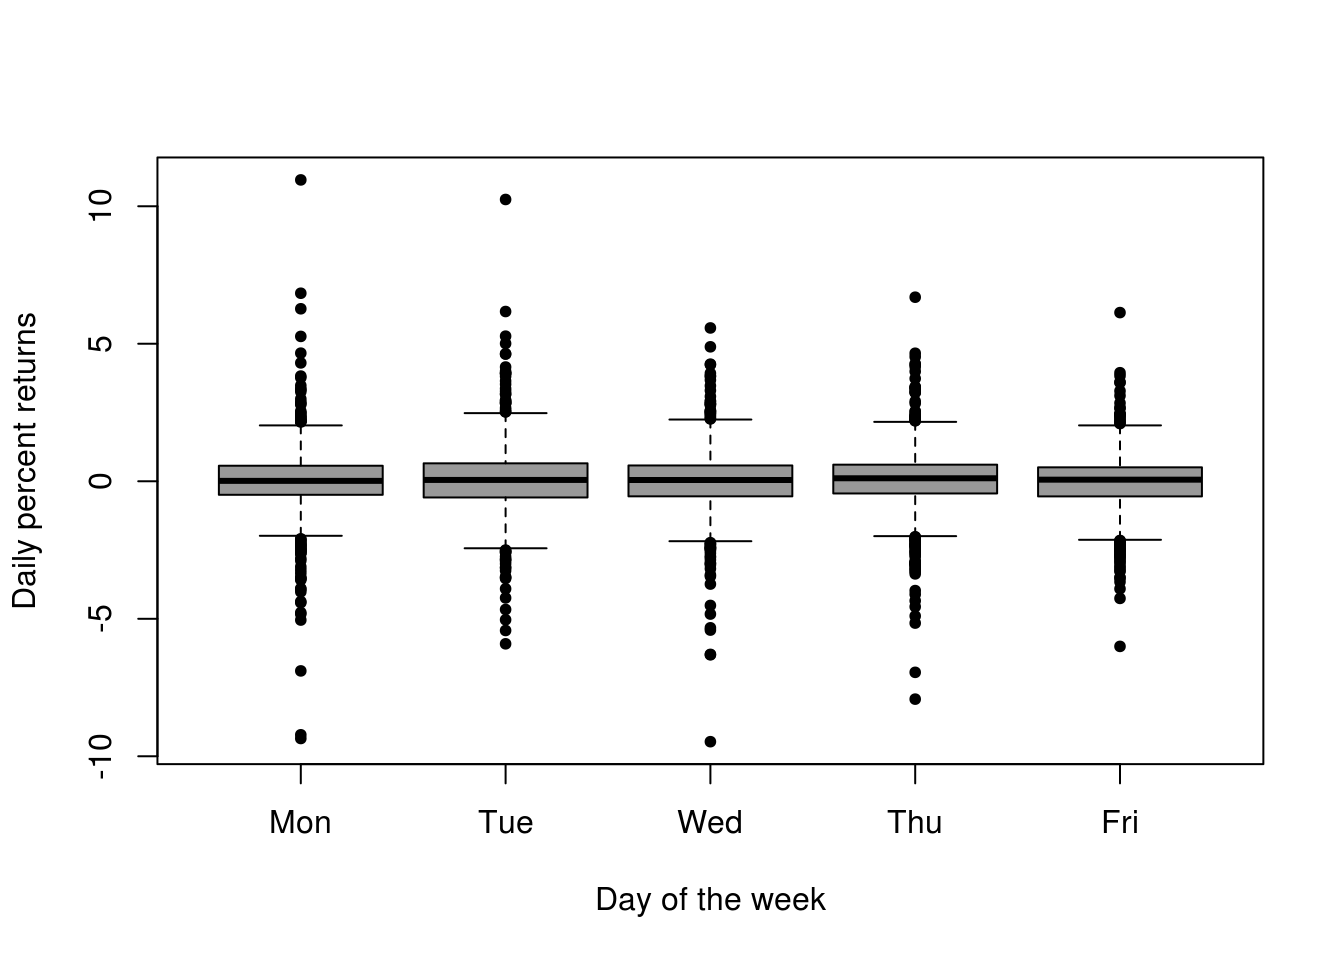
\includegraphics{timeseRies_files/figure-latex/Question_2-3.pdf}

\begin{Shaded}
\begin{Highlighting}[]
\CommentTok{# More uncertainty in March-May and August-November Some more extremes early}
\CommentTok{# in the week}

\KeywordTok{par}\NormalTok{(}\DataTypeTok{mfrow =} \KeywordTok{c}\NormalTok{(}\DecValTok{1}\NormalTok{, }\DecValTok{2}\NormalTok{))}
\NormalTok{title_sp <-}\StringTok{ "Daily return of }\CharTok{\textbackslash{}n}\StringTok{adjusted SP500 at closure"}
\NormalTok{TSA}\OperatorTok{::}\KeywordTok{acf}\NormalTok{(spret, }\DataTypeTok{na.action =}\NormalTok{ na.pass, }\DataTypeTok{main =}\NormalTok{ title_sp)}
\NormalTok{TSA}\OperatorTok{::}\KeywordTok{acf}\NormalTok{(}\KeywordTok{na.omit}\NormalTok{(}\KeywordTok{as.vector}\NormalTok{(spret)), }\DataTypeTok{main =}\NormalTok{ title_sp)}
\end{Highlighting}
\end{Shaded}

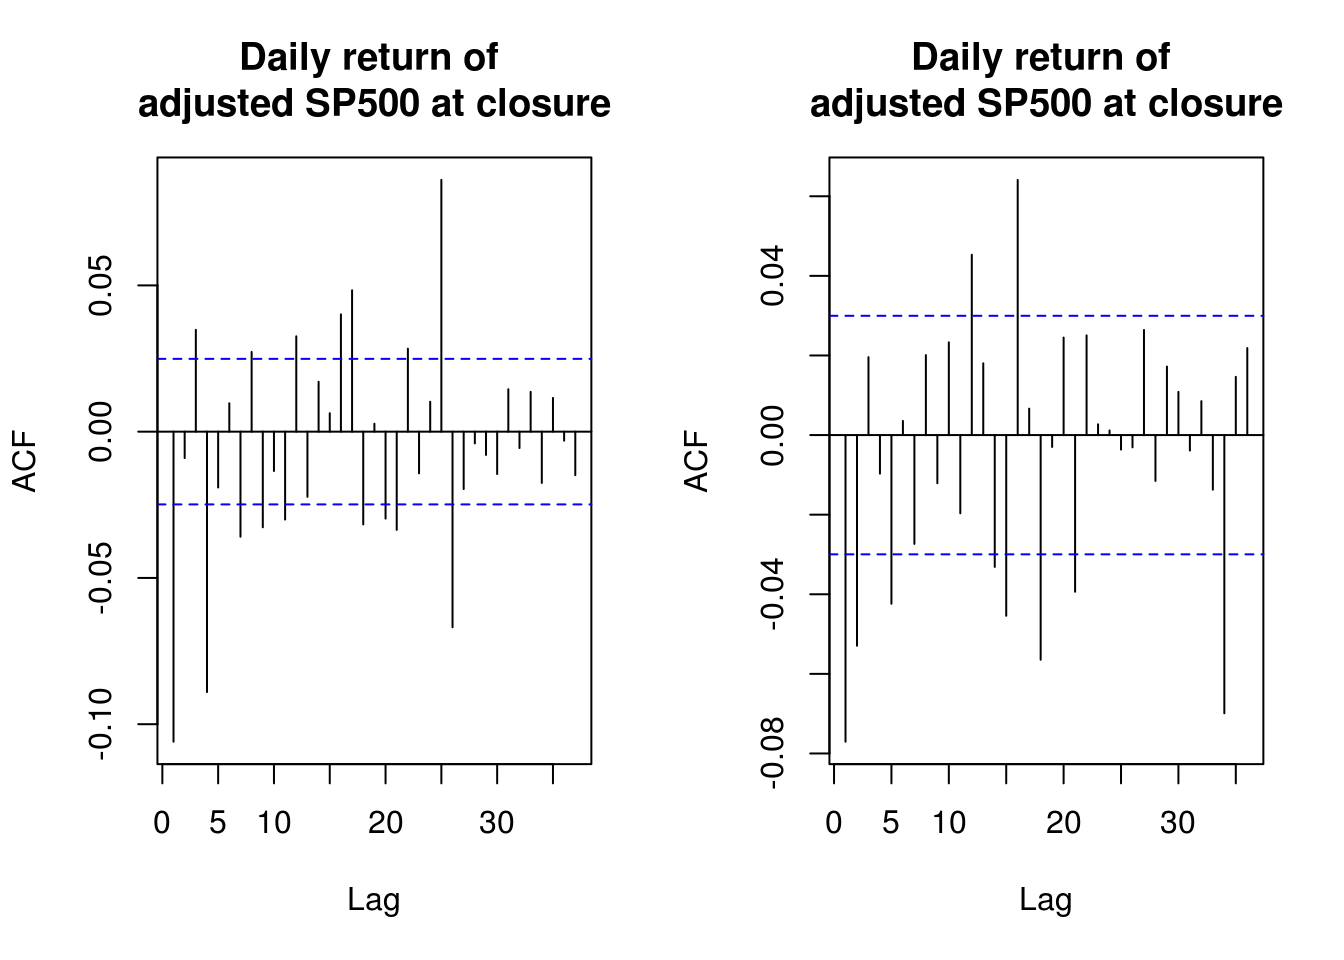
\includegraphics{timeseRies_files/figure-latex/Question_2-4.pdf}

\begin{Shaded}
\begin{Highlighting}[]
\KeywordTok{dev.off}\NormalTok{()}
\end{Highlighting}
\end{Shaded}

\begin{verbatim}
null device 
          1 
\end{verbatim}

\begin{Shaded}
\begin{Highlighting}[]
\KeywordTok{pacf}\NormalTok{(spret, }\DataTypeTok{na.action =}\NormalTok{ na.pass, }\DataTypeTok{main =}\NormalTok{ title_sp)}

\CommentTok{# (P)ACF of absolute value of daily returns}
\NormalTok{TSA}\OperatorTok{::}\KeywordTok{acf}\NormalTok{(}\KeywordTok{abs}\NormalTok{(spret), }\DataTypeTok{na.action =}\NormalTok{ na.pass, }\DataTypeTok{main =}\NormalTok{ title_sp)}
\KeywordTok{pacf}\NormalTok{(}\KeywordTok{abs}\NormalTok{(spret), }\DataTypeTok{na.action =}\NormalTok{ na.pass, }\DataTypeTok{main =}\NormalTok{ title_sp)}
\CommentTok{# (P)ACF of squared daily returns}
\NormalTok{TSA}\OperatorTok{::}\KeywordTok{acf}\NormalTok{(}\KeywordTok{I}\NormalTok{(spret}\OperatorTok{^}\DecValTok{2}\NormalTok{), }\DataTypeTok{na.action =}\NormalTok{ na.pass, }\DataTypeTok{main =}\NormalTok{ title_sp)}
\KeywordTok{pacf}\NormalTok{(}\KeywordTok{I}\NormalTok{(spret}\OperatorTok{^}\DecValTok{2}\NormalTok{), }\DataTypeTok{na.action =}\NormalTok{ na.pass, }\DataTypeTok{main =}\NormalTok{ title_sp)}
\end{Highlighting}
\end{Shaded}

\subsection{Solutions 3: Simulated
data}\label{solutions-3-simulated-data}

The first 5 parts of the question are straightforward and left to the
reader.

\begin{enumerate}
\def\labelenumi{\arabic{enumi}.}
\tightlist
\item
  Simulate 500 observations from an AR(1) process with parameter values
  \(\alpha \in \{0.1, 0.5, 0.9, 0.99\}\).
\item
  Repeat for MA processes of different orders. There is no restriction
  on the coefficients of the latter for stationarity, unlike the AR
  process.
\item
  Sample from an ARCH(1) process with Gaussian innovations and an
  ARCH(1) process with Student-\(t\) innovations with \texttt{df=4}.
  Look at the correlogram of the absolute residuals and the squared
  residuals.
\item
  The dataset \texttt{EuStockMarkets} contains the daily closing prices
  of major European stock indices. Type \texttt{?EuStockMarkets} for
  more details and \texttt{plot(EuStockMarkets)} to plot the four series
  (DAX, SMI, CAC and FTSE). Use
  \texttt{plot(ftse\ \textless{}-\ EuStockMarkets{[},"FTSE"{]})} to plot
  the FTSE series and \texttt{plot(100*diff(log(ftse)))} to plot its
  daily log return. Play with the ARCH simulation functions to generate
  some similar processes.
\item
  Simulate a white noise series with trend \(t\) and \(\cos(t)\), of the
  form \(X_t=M_t+S_t+Z_t\), where \(Z_t \sim \mathsf{N}(0,\sigma^2)\)
  for different values of \(\sigma^2\). Analyze the log-periodogram and
  the (partial) correlograms. What happens if you forget to remove the
  trend?
\item
  Do the same for multiplicative model with lognormal margins, with
  structure \(X_t=M_tS_tZ_t\).
\item
  For steps 5 and 6, plot the series and test the assumptions that they
  are white noise using the Ljung-Box test. \emph{Note} you need to
  adjust the degrees of freedom when working with residuals from
  e.g.~ARMA models.
\end{enumerate}

\begin{Shaded}
\begin{Highlighting}[]
\NormalTok{n <-}\StringTok{ }\DecValTok{100}
\NormalTok{tim <-}\StringTok{ }\KeywordTok{scale}\NormalTok{(}\DecValTok{1}\OperatorTok{:}\NormalTok{n)}
\NormalTok{x <-}\StringTok{ }\DecValTok{5} \OperatorTok{*}\StringTok{ }\NormalTok{tim }\OperatorTok{+}\StringTok{ }\KeywordTok{cos}\NormalTok{(}\DecValTok{2} \OperatorTok{*}\StringTok{ }\NormalTok{pi }\OperatorTok{*}\StringTok{ }\NormalTok{tim}\OperatorTok{/}\NormalTok{n) }\OperatorTok{+}\StringTok{ }\KeywordTok{rnorm}\NormalTok{(n, }\DataTypeTok{sd =} \DecValTok{3}\NormalTok{)}
\KeywordTok{plot}\NormalTok{(x, }\DataTypeTok{type =} \StringTok{"l"}\NormalTok{, }\DataTypeTok{main =} \StringTok{"Simulated series with seasonality and trend"}\NormalTok{)}
\end{Highlighting}
\end{Shaded}

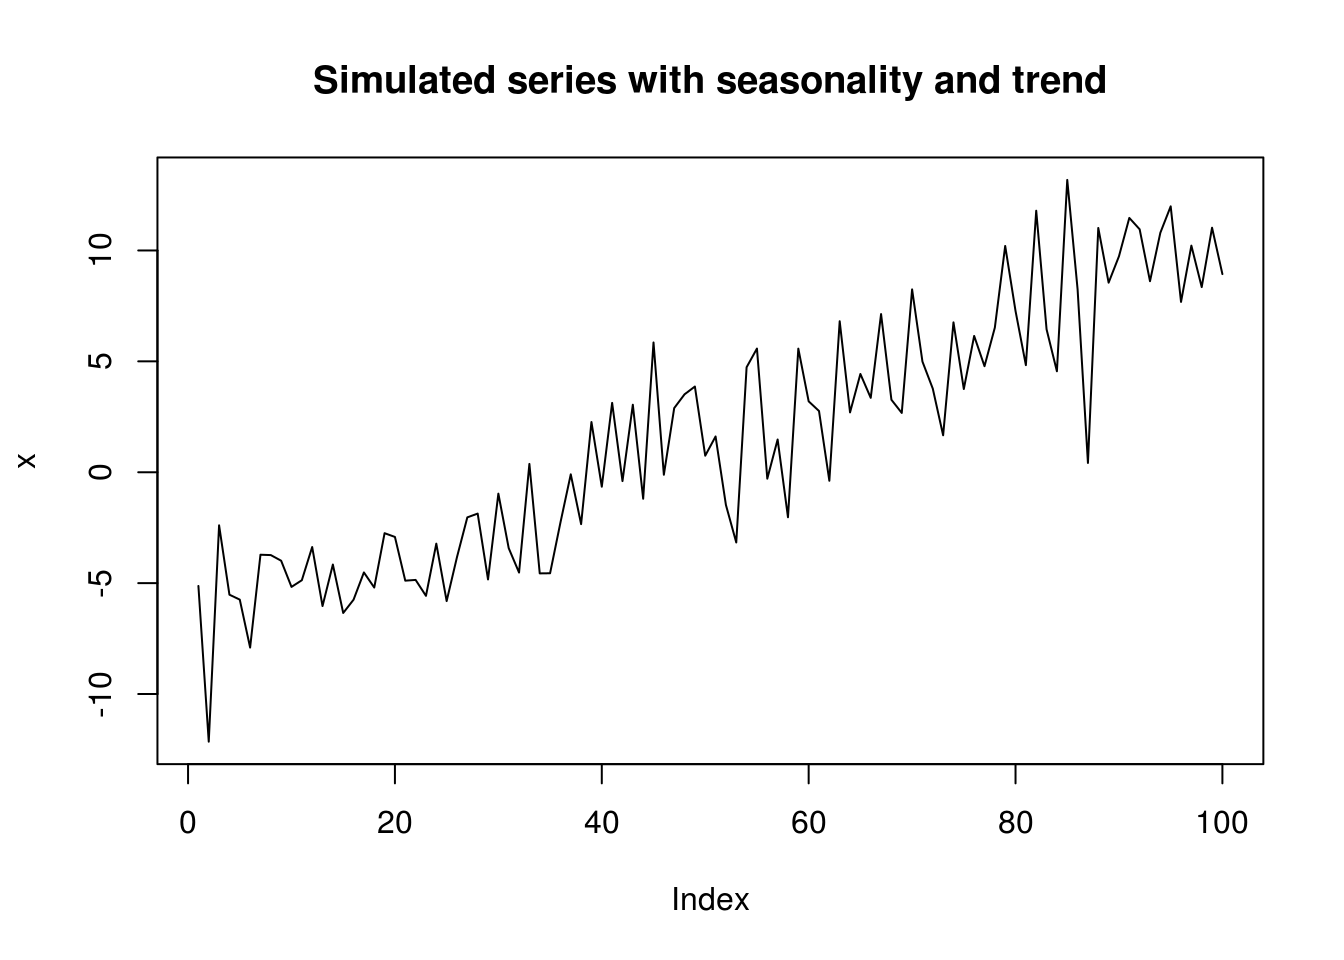
\includegraphics{timeseRies_files/figure-latex/Question_3-1.pdf}

\begin{Shaded}
\begin{Highlighting}[]
\KeywordTok{Box.test}\NormalTok{(x, }\DataTypeTok{type =} \StringTok{"L"}\NormalTok{)}
\end{Highlighting}
\end{Shaded}

\begin{verbatim}

    Box-Ljung test

data:  x
X-squared = 61.616, df = 1, p-value = 4.219e-15
\end{verbatim}

\begin{Shaded}
\begin{Highlighting}[]
\KeywordTok{par}\NormalTok{(}\DataTypeTok{mfrow =} \KeywordTok{c}\NormalTok{(}\DecValTok{1}\NormalTok{, }\DecValTok{3}\NormalTok{))  }\CommentTok{# plots side by side}
\NormalTok{TSA}\OperatorTok{::}\KeywordTok{acf}\NormalTok{(x, }\DataTypeTok{main =} \StringTok{"Simulated series"}\NormalTok{)}
\KeywordTok{pacf}\NormalTok{(x, }\DataTypeTok{main =} \StringTok{"Simulated series"}\NormalTok{)}
\KeywordTok{spectrum}\NormalTok{(x, }\DataTypeTok{main =} \StringTok{"Simulated series"}\NormalTok{)}
\end{Highlighting}
\end{Shaded}

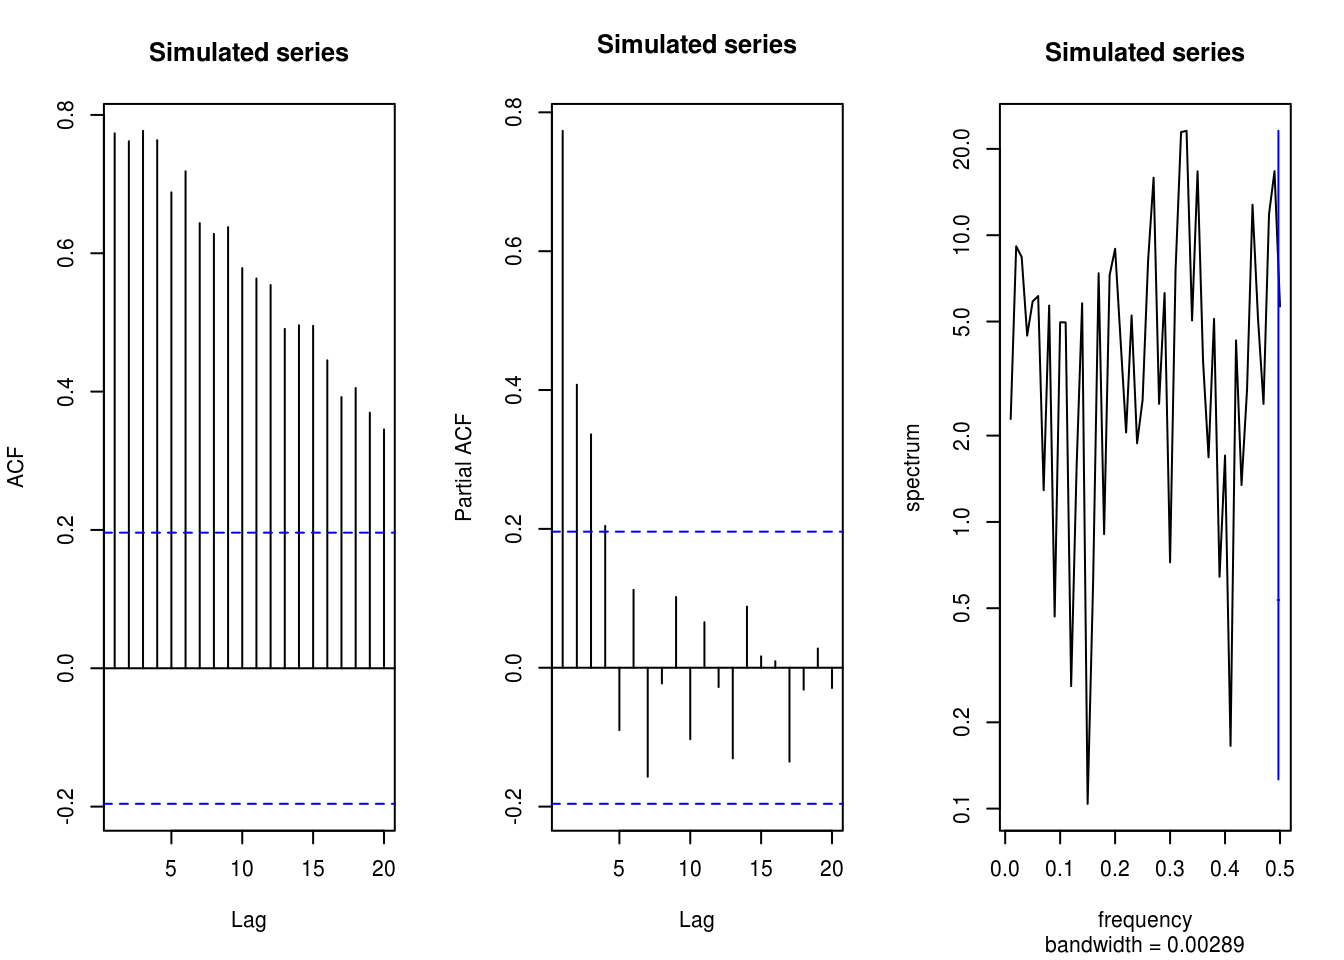
\includegraphics{timeseRies_files/figure-latex/Question_3-2.pdf}

\begin{Shaded}
\begin{Highlighting}[]
\CommentTok{# Nothing in spectrum, persistence in the (p)acf}
\NormalTok{x <-}\StringTok{ }\DecValTok{5} \OperatorTok{*}\StringTok{ }\NormalTok{tim }\OperatorTok{+}\StringTok{ }\KeywordTok{cos}\NormalTok{(}\DecValTok{2} \OperatorTok{*}\StringTok{ }\NormalTok{pi }\OperatorTok{*}\StringTok{ }\NormalTok{tim}\OperatorTok{/}\NormalTok{n) }\OperatorTok{+}\StringTok{ }\KeywordTok{rnorm}\NormalTok{(n, }\DataTypeTok{sd =} \FloatTok{0.5}\NormalTok{)}
\NormalTok{TSA}\OperatorTok{::}\KeywordTok{acf}\NormalTok{(x, }\DataTypeTok{main =} \StringTok{"Simulated series"}\NormalTok{)}
\KeywordTok{pacf}\NormalTok{(x, }\DataTypeTok{main =} \StringTok{"Simulated series"}\NormalTok{)}
\KeywordTok{spectrum}\NormalTok{(x, }\DataTypeTok{main =} \StringTok{"Simulated series"}\NormalTok{)}
\end{Highlighting}
\end{Shaded}

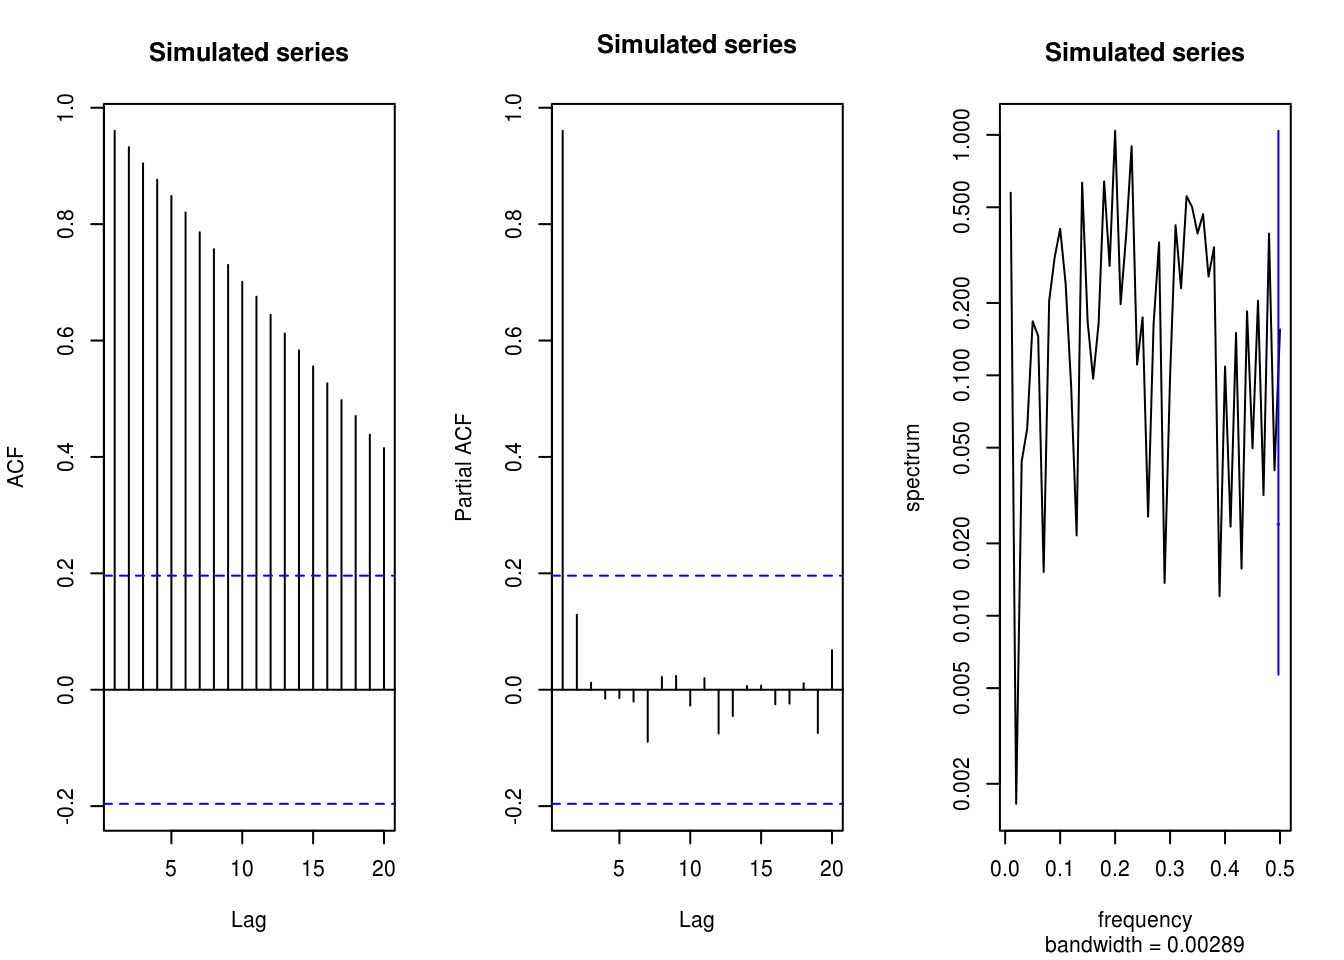
\includegraphics{timeseRies_files/figure-latex/Question_3-3.pdf}

\begin{Shaded}
\begin{Highlighting}[]
\CommentTok{# Worst if the signal is strong relative to noise}

\NormalTok{y <-}\StringTok{ }\KeywordTok{residuals}\NormalTok{(}\KeywordTok{lm}\NormalTok{(x }\OperatorTok{~}\StringTok{ }\DecValTok{1} \OperatorTok{+}\StringTok{ }\NormalTok{tim))}
\NormalTok{TSA}\OperatorTok{::}\KeywordTok{acf}\NormalTok{(y, }\DataTypeTok{main =} \StringTok{"Detrended series"}\NormalTok{)}
\KeywordTok{pacf}\NormalTok{(x, }\DataTypeTok{main =} \StringTok{"Detrended series"}\NormalTok{)}
\KeywordTok{spectrum}\NormalTok{(y, }\DataTypeTok{main =} \StringTok{"Detrended series"}\NormalTok{)}
\end{Highlighting}
\end{Shaded}

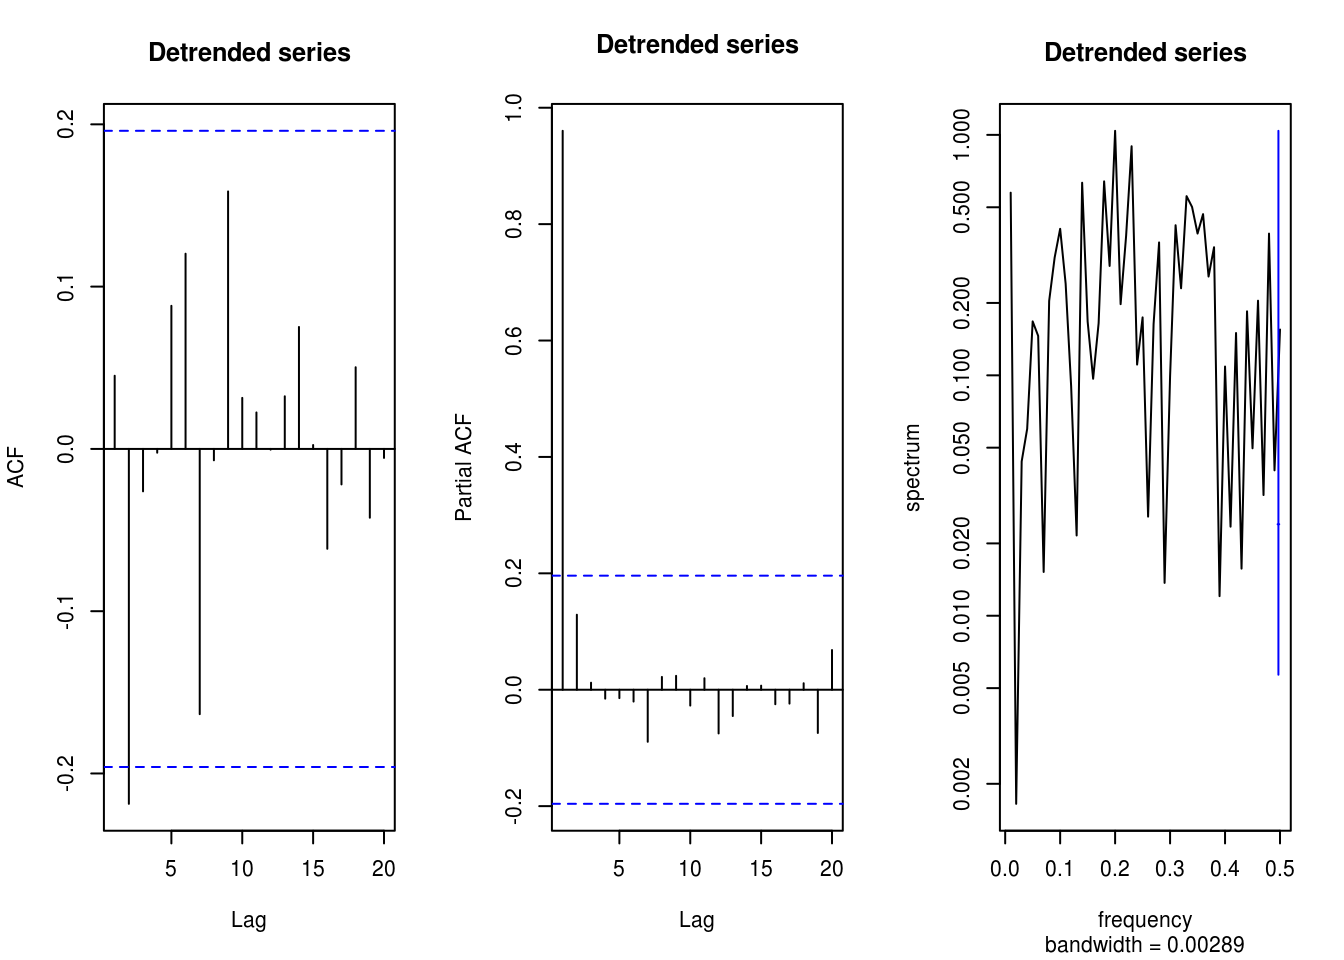
\includegraphics{timeseRies_files/figure-latex/Question_3-4.pdf}

\begin{Shaded}
\begin{Highlighting}[]
\CommentTok{# The cosine still induces some lag-one dependence in pacf}
\KeywordTok{plot}\NormalTok{(}\DecValTok{1}\OperatorTok{:}\DecValTok{10}\NormalTok{, }\KeywordTok{sapply}\NormalTok{(}\DecValTok{1}\OperatorTok{:}\DecValTok{10}\NormalTok{, }\ControlFlowTok{function}\NormalTok{(i) \{}
    \KeywordTok{Box.test}\NormalTok{(y, }\DataTypeTok{lag =}\NormalTok{ i, }\DataTypeTok{type =} \StringTok{"Ljung"}\NormalTok{, }\DataTypeTok{fitdf =} \KeywordTok{min}\NormalTok{(i }\OperatorTok{-}\StringTok{ }\DecValTok{1}\NormalTok{, }\DecValTok{2}\NormalTok{))}\OperatorTok{$}\NormalTok{p.value}
\NormalTok{\}), }\DataTypeTok{ylab =} \StringTok{"P-value"}\NormalTok{, }\DataTypeTok{xlab =} \StringTok{"lag"}\NormalTok{)}
\CommentTok{# These low p-values at large lags are due to the cosine term}

\NormalTok{mult <-}\StringTok{ }\KeywordTok{exp}\NormalTok{(}\KeywordTok{scale}\NormalTok{(x))}
\NormalTok{TSA}\OperatorTok{::}\KeywordTok{acf}\NormalTok{(mult, }\DataTypeTok{main =} \StringTok{"Multiplicative series"}\NormalTok{)}
\KeywordTok{pacf}\NormalTok{(mult, }\DataTypeTok{main =} \StringTok{"Multiplicative series"}\NormalTok{)}
\end{Highlighting}
\end{Shaded}

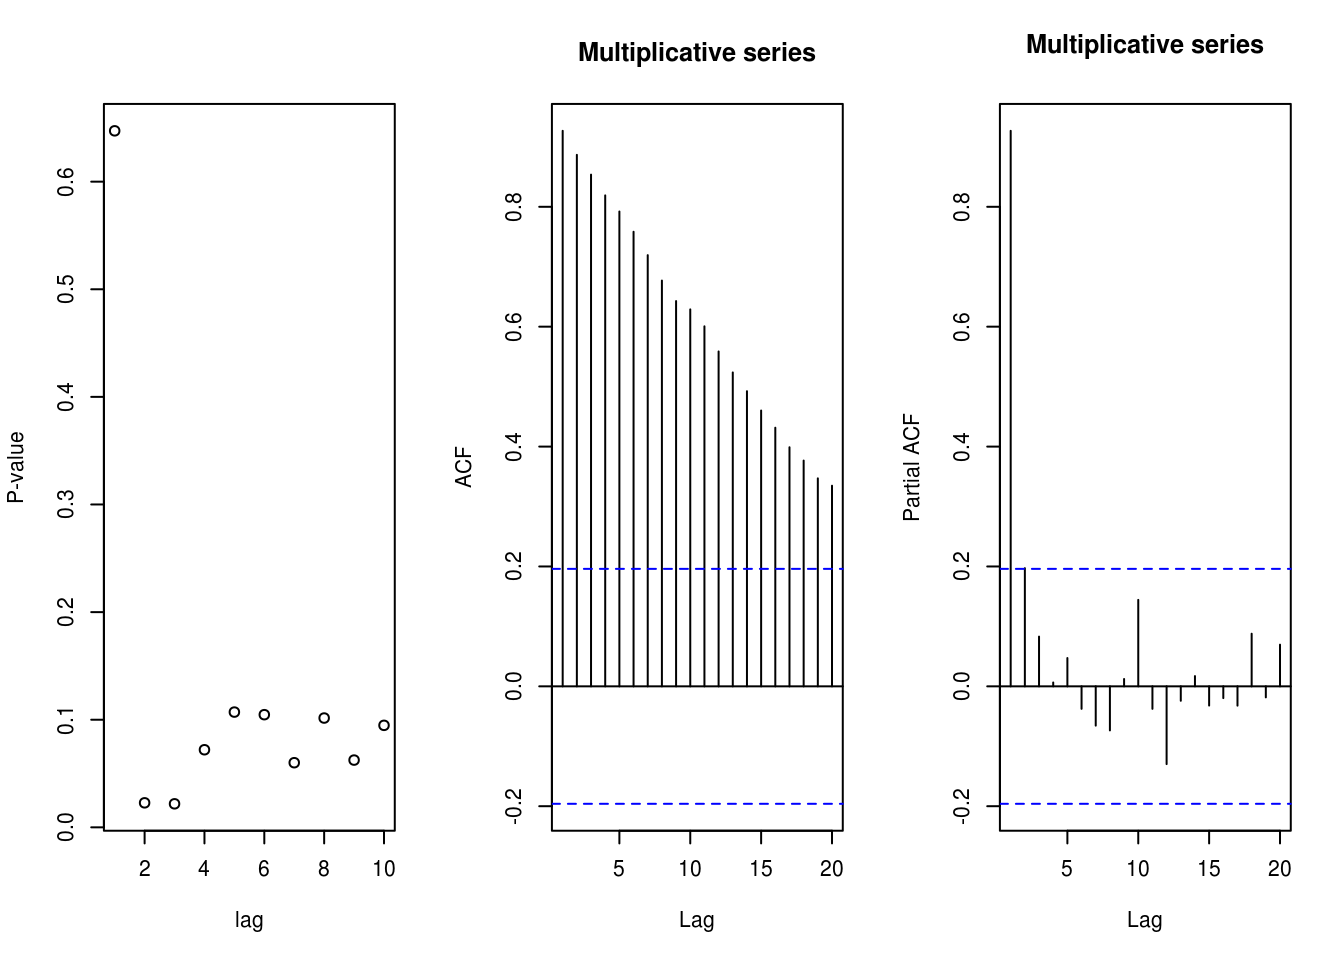
\includegraphics{timeseRies_files/figure-latex/Question_3-5.pdf}

\begin{Shaded}
\begin{Highlighting}[]
\KeywordTok{spectrum}\NormalTok{(mult, }\DataTypeTok{main =} \StringTok{"Multiplicative series"}\NormalTok{)}
\KeywordTok{Box.test}\NormalTok{(mult, }\DataTypeTok{type =} \StringTok{"L"}\NormalTok{)}
\end{Highlighting}
\end{Shaded}

\begin{verbatim}

    Box-Ljung test

data:  mult
X-squared = 88.489, df = 1, p-value < 2.2e-16
\end{verbatim}

\begin{Shaded}
\begin{Highlighting}[]
\KeywordTok{graphics.off}\NormalTok{()}
\CommentTok{# Now large impact on spectrum, and nonlinear features!}
\KeywordTok{plot}\NormalTok{(mult, }\DataTypeTok{main =} \StringTok{"Multiplicative series with lognormal margins"}\NormalTok{, }\DataTypeTok{ylab =} \StringTok{""}\NormalTok{, }
    \DataTypeTok{xlab =} \StringTok{"Time"}\NormalTok{)}
\CommentTok{# Note that decompose has an option type='multiplicative' for seasonal}
\CommentTok{# components}
\end{Highlighting}
\end{Shaded}

\subsection{\texorpdfstring{Solutions 4: Mauna Loa Atmospheric
CO\textsubscript{2}
Concentration}{Solutions 4: Mauna Loa Atmospheric CO2 Concentration}}\label{solutions-4-mauna-loa-atmospheric-co2-concentration}

\begin{enumerate}
\def\labelenumi{\arabic{enumi}.}
\tightlist
\item
  Load and plot the CO\textsubscript{2} dataset from
  \href{ftp://aftp.cmdl.noaa.gov/products/trends/co2/co2_mm_mlo.txt}{NOAA}.
  Pay special attention to the format, missing values, the handling of
  string and the description. Use \texttt{?read.table} for help, and
  look carefully at arguments \texttt{file}, \texttt{sep},
  \texttt{na.strings}, \texttt{skip} and \texttt{stringsAsFactors}. From
  now on, we will work with the complete series (termed interpolated in
  the description).
\item
  Try removing the trend using a linear model. Plot the residuals
  against month of the year.
\item
  Remove the trend and the periodicity with a Fourier basis (with period
  12). Be sure to include both \texttt{sin} and \texttt{cos} terms
  together. Recall that the standard Wald tests for the coefficients is
  not valid in the presence of autocorrelation! You could also use
  \texttt{poly} or \texttt{splines::bs} to fit polynomials or splines to
  your series.
\item
  Plot the lagged residuals. Are there evidence of correlation?
\item
  Use the function \texttt{filter} to smooth the series using a 12
  period moving average.
\item
  Inspect the spectrum of the raw series and of the smoothed version.
\item
  Inspect the spectrum of the detrended raw series.
\item
  Test for stationarity of the deseasonalized and detrended residuals
  using the KPSS test viz. \texttt{tseries::kpss.test}.
\item
  Use the \texttt{decompose} and the \texttt{stl} functions to obtain
  residuals.
\item
  Plot the (partial) correlogram for both decomposition and compare them
  with the output of the linear model.
\end{enumerate}

\begin{Shaded}
\begin{Highlighting}[]
\CommentTok{# Because of comment.char=#, all the first lines are skipped But we lose the}
\CommentTok{# header}
\NormalTok{co2 <-}\StringTok{ }\KeywordTok{read.table}\NormalTok{(}\DataTypeTok{file =} \StringTok{"ftp://aftp.cmdl.noaa.gov/products/trends/co2/co2_mm_mlo.txt"}\NormalTok{, }
    \DataTypeTok{na.strings =} \StringTok{"-99.99"}\NormalTok{, }\DataTypeTok{stringsAsFactors =} \OtherTok{FALSE}\NormalTok{, }\DataTypeTok{col.names =} \KeywordTok{c}\NormalTok{(}\StringTok{"year"}\NormalTok{, }\StringTok{"month"}\NormalTok{, }
        \StringTok{"time"}\NormalTok{, }\StringTok{"average"}\NormalTok{, }\StringTok{"interpolated"}\NormalTok{, }\StringTok{"trend"}\NormalTok{, }\StringTok{"monthly_mean"}\NormalTok{))}
\CommentTok{# install.packages('stlplus') #this package offers a version of stl that}
\CommentTok{# deals with NAs}

\NormalTok{ycap <-}\StringTok{ }\KeywordTok{expression}\NormalTok{(}\KeywordTok{paste}\NormalTok{(}\StringTok{"Monthly mean "}\NormalTok{, CO[}\DecValTok{2}\NormalTok{], }\StringTok{" mole fraction (ppm)"}\NormalTok{))}
\NormalTok{mcap <-}\StringTok{ "Average monthly mean CO2 concentration}\CharTok{\textbackslash{}n}\StringTok{ determined from daily averages"}
\NormalTok{lin_mod <-}\StringTok{ }\KeywordTok{lm}\NormalTok{(}\DataTypeTok{data =}\NormalTok{ co2, interpolated }\OperatorTok{~}\StringTok{ }\NormalTok{time)}
\KeywordTok{with}\NormalTok{(co2, }\KeywordTok{plot}\NormalTok{(interpolated }\OperatorTok{~}\StringTok{ }\NormalTok{time, }\DataTypeTok{type =} \StringTok{"l"}\NormalTok{, }\DataTypeTok{xlab =} \StringTok{"Time"}\NormalTok{, }\DataTypeTok{bty =} \StringTok{"l"}\NormalTok{, }\DataTypeTok{ylab =}\NormalTok{ ycap, }
    \DataTypeTok{main =}\NormalTok{ mcap))}
\end{Highlighting}
\end{Shaded}

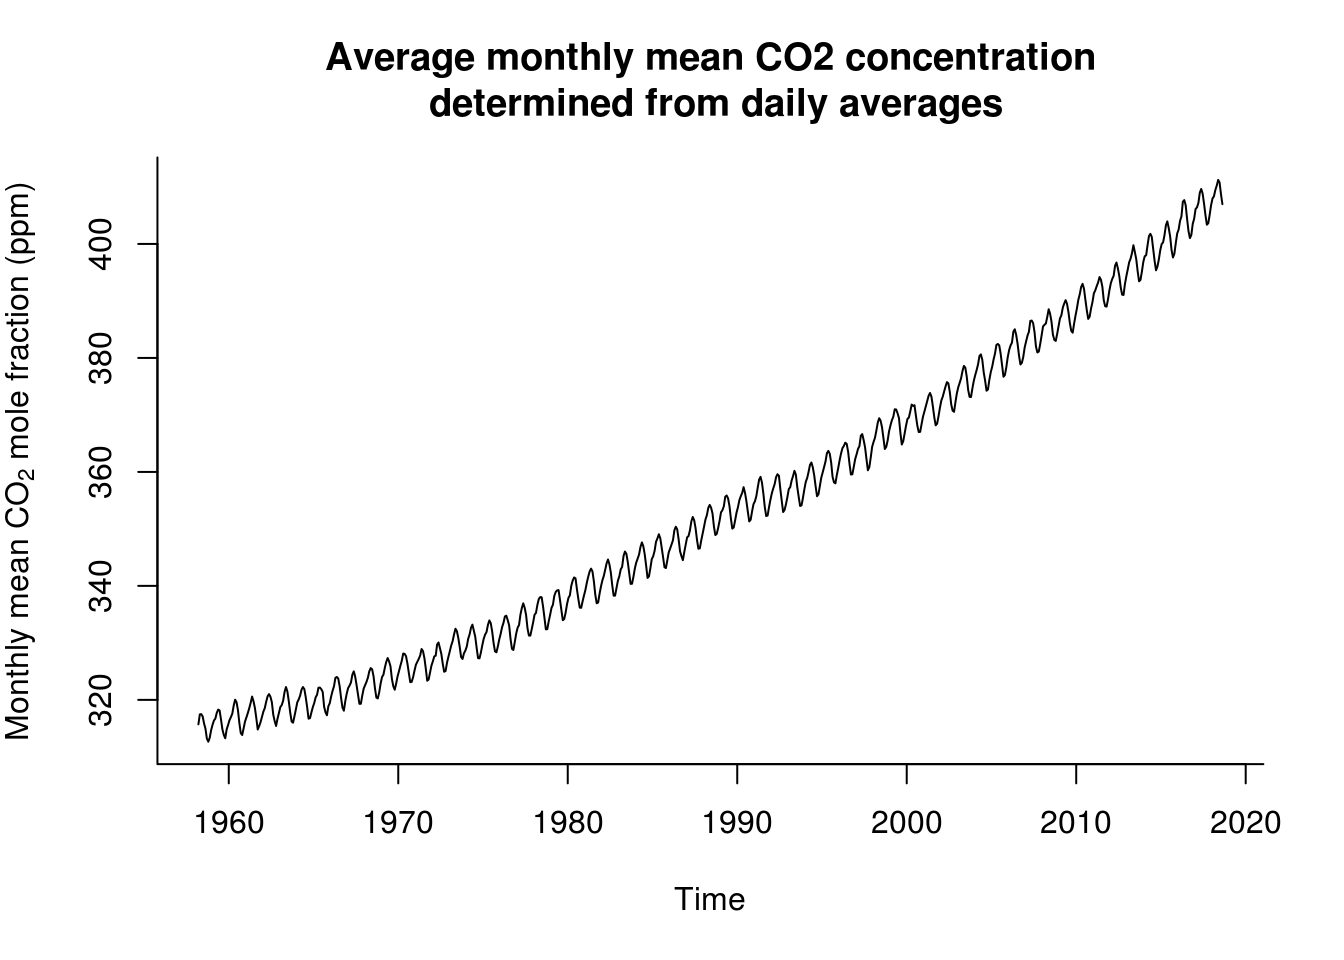
\includegraphics{timeseRies_files/figure-latex/Question_4-1.pdf}

\begin{Shaded}
\begin{Highlighting}[]
\KeywordTok{plot}\NormalTok{(co2}\OperatorTok{$}\NormalTok{time, }\KeywordTok{residuals}\NormalTok{(lin_mod), }\DataTypeTok{ylab =} \StringTok{"Residual from `lm` (linear trend)"}\NormalTok{, }
    \DataTypeTok{xlab =} \StringTok{"Time"}\NormalTok{, }\DataTypeTok{main =}\NormalTok{ mcap)}
\end{Highlighting}
\end{Shaded}

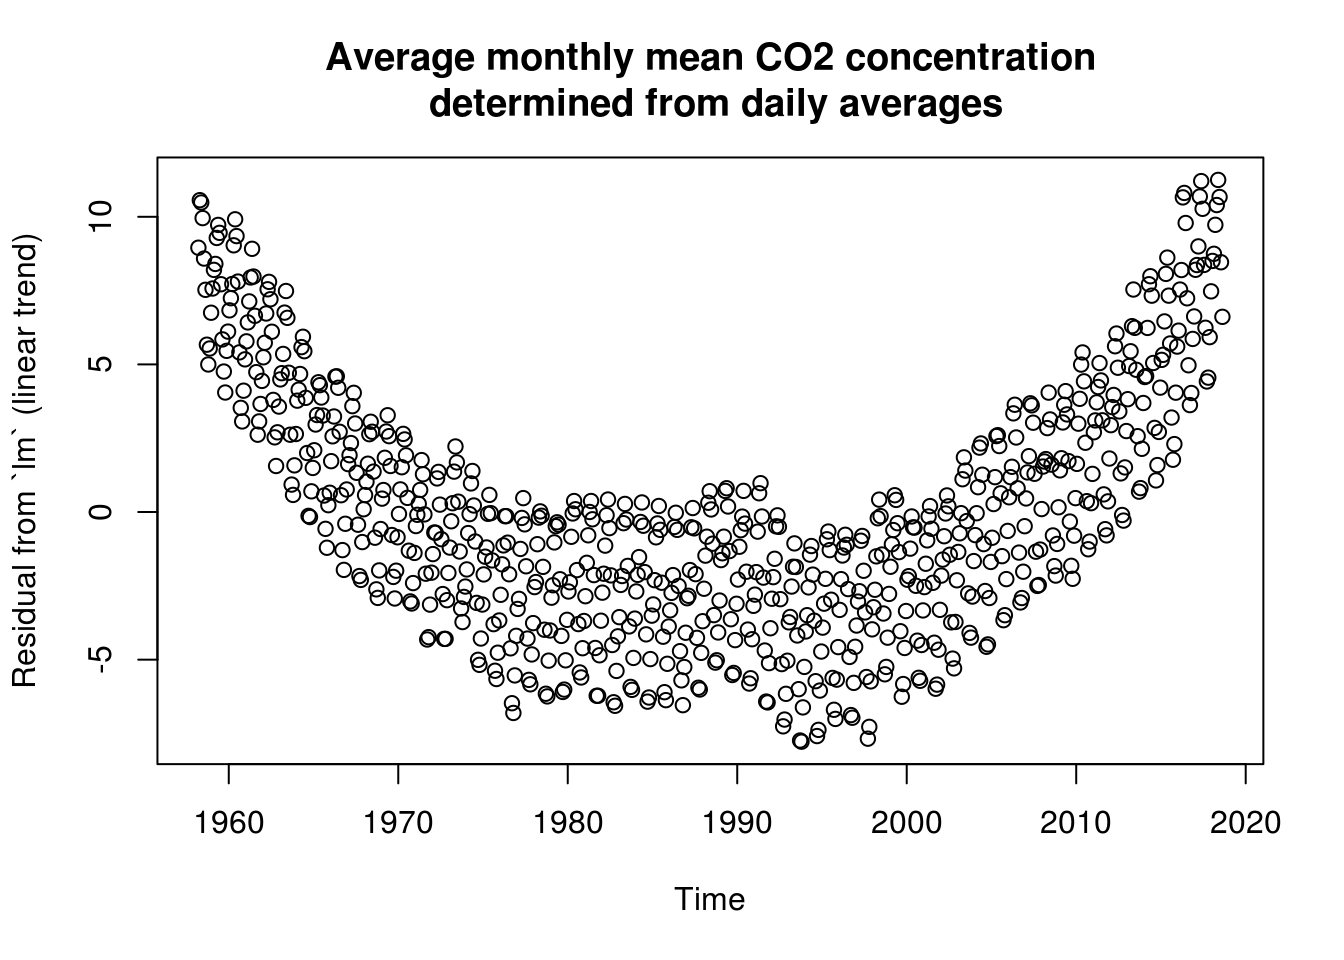
\includegraphics{timeseRies_files/figure-latex/Question_4-2.pdf}

\begin{Shaded}
\begin{Highlighting}[]
\NormalTok{lin_mod <-}\StringTok{ }\KeywordTok{update}\NormalTok{(lin_mod, . }\OperatorTok{~}\StringTok{ }\NormalTok{. }\OperatorTok{+}\StringTok{ }\KeywordTok{I}\NormalTok{(time}\OperatorTok{^}\DecValTok{2}\NormalTok{))}
\CommentTok{# same as lm(data=co2, interpolated ~ poly(time, degree = 2))}
\KeywordTok{plot}\NormalTok{(co2}\OperatorTok{$}\NormalTok{time, }\KeywordTok{residuals}\NormalTok{(lin_mod), }\DataTypeTok{main =}\NormalTok{ mcap, }\DataTypeTok{ylab =} \StringTok{"Residual from `lm` (quadratic trend)"}\NormalTok{, }
    \DataTypeTok{xlab =} \StringTok{"Time"}\NormalTok{)}
\end{Highlighting}
\end{Shaded}

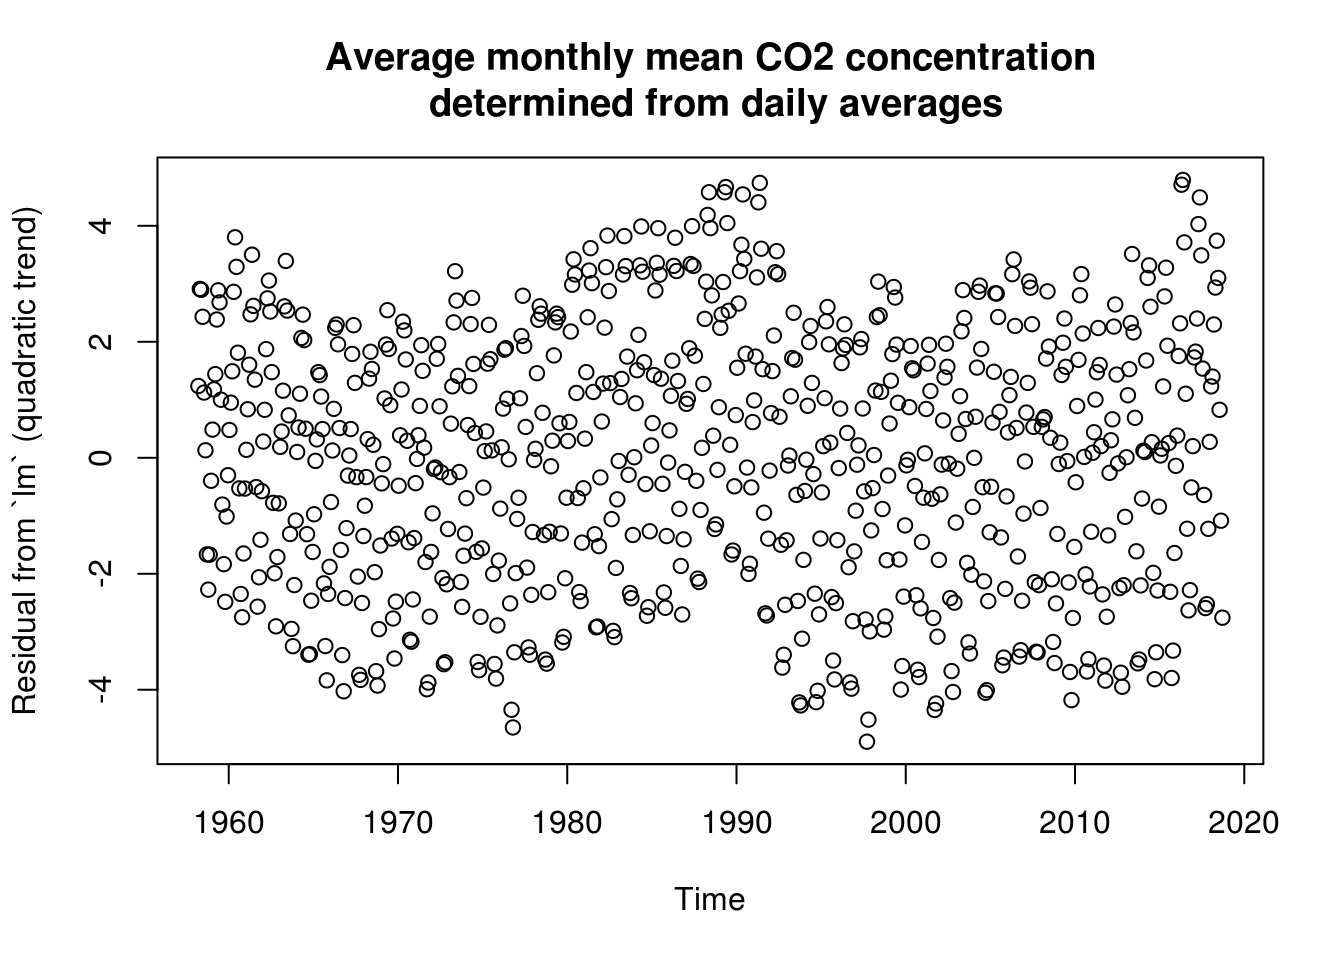
\includegraphics{timeseRies_files/figure-latex/Question_4-3.pdf}

\begin{Shaded}
\begin{Highlighting}[]
\CommentTok{# Cast the full time series into a ts object}
\NormalTok{co2_ts <-}\StringTok{ }\KeywordTok{with}\NormalTok{(co2, }\KeywordTok{ts}\NormalTok{(}\DataTypeTok{data =}\NormalTok{ interpolated, }\DataTypeTok{start =} \KeywordTok{c}\NormalTok{(year[}\DecValTok{1}\NormalTok{], month[}\DecValTok{1}\NormalTok{]), }\DataTypeTok{end =} \KeywordTok{c}\NormalTok{(}\KeywordTok{tail}\NormalTok{(year, }
    \DecValTok{1}\NormalTok{), }\KeywordTok{tail}\NormalTok{(month, }\DecValTok{1}\NormalTok{)), }\DataTypeTok{frequency =} \DecValTok{12}\NormalTok{))}
\KeywordTok{with}\NormalTok{(co2, }\KeywordTok{plot}\NormalTok{(}\KeywordTok{jitter}\NormalTok{(month, }\DecValTok{1}\OperatorTok{/}\DecValTok{3}\NormalTok{), }\KeywordTok{residuals}\NormalTok{(lin_mod), }\DataTypeTok{ylab =} \StringTok{"Residuals"}\NormalTok{, }\DataTypeTok{xlab =} \StringTok{"Month of year"}\NormalTok{, }
    \DataTypeTok{main =}\NormalTok{ mcap))}
\end{Highlighting}
\end{Shaded}

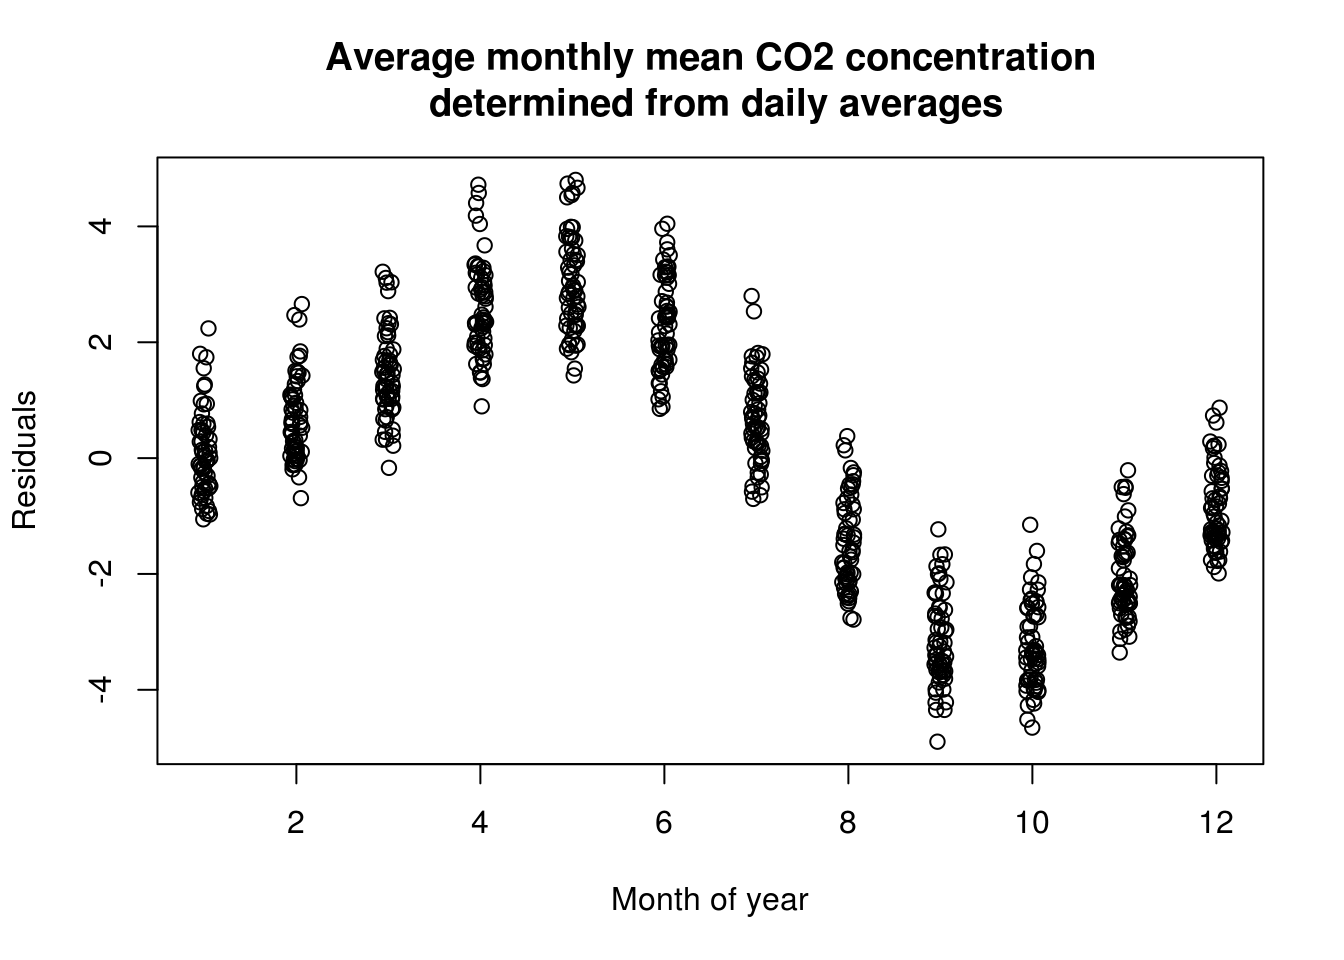
\includegraphics{timeseRies_files/figure-latex/Question_4-4.pdf}

\begin{Shaded}
\begin{Highlighting}[]
\CommentTok{# Could create the basis manually}
\NormalTok{f_bs <-}\StringTok{ }\KeywordTok{with}\NormalTok{(co2, fda}\OperatorTok{::}\KeywordTok{fourier}\NormalTok{(month, }\DataTypeTok{nbasis =} \DecValTok{4}\NormalTok{, }\DataTypeTok{period =} \DecValTok{12}\NormalTok{))[, }\OperatorTok{-}\DecValTok{1}\NormalTok{]}
\NormalTok{lin_mod <-}\StringTok{ }\KeywordTok{with}\NormalTok{(co2, }\KeywordTok{lm}\NormalTok{(interpolated }\OperatorTok{~}\StringTok{ }\NormalTok{splines}\OperatorTok{::}\KeywordTok{bs}\NormalTok{(time, }\DataTypeTok{df =} \DecValTok{5}\NormalTok{, }\DataTypeTok{degree =} \DecValTok{3}\NormalTok{) }\OperatorTok{+}\StringTok{ }
\StringTok{    }\NormalTok{f_bs))}
\CommentTok{# summary(lin_mod) Is there structure left in the residuals?}
\KeywordTok{plot}\NormalTok{(co2}\OperatorTok{$}\NormalTok{time, }\KeywordTok{residuals}\NormalTok{(lin_mod), }\DataTypeTok{ylab =} \StringTok{"Residuals from final `lm` model"}\NormalTok{, }
    \DataTypeTok{xlab =} \StringTok{"Time"}\NormalTok{, }\DataTypeTok{main =}\NormalTok{ mcap)}
\end{Highlighting}
\end{Shaded}

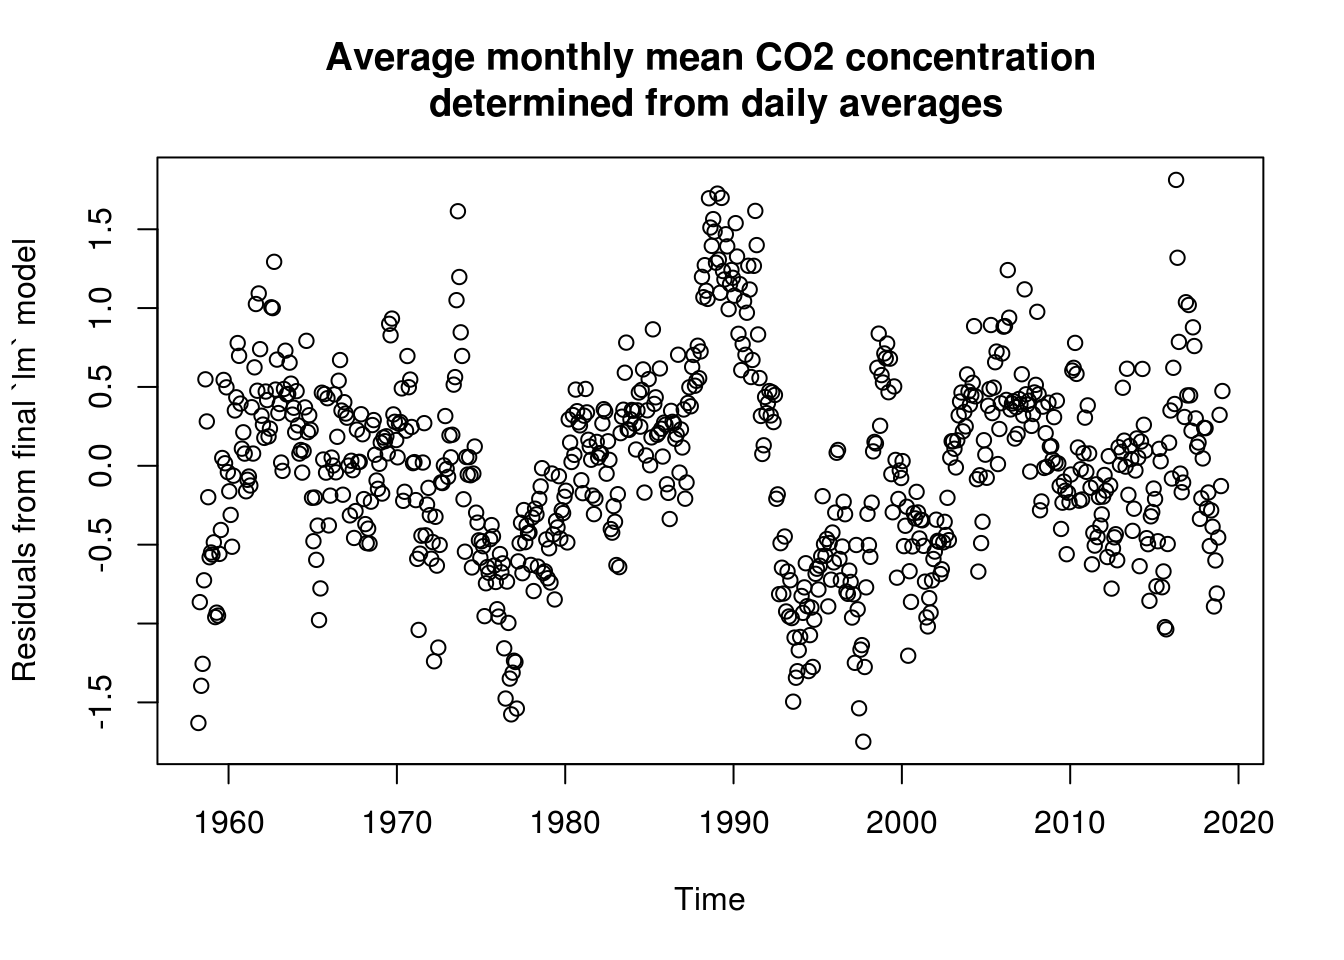
\includegraphics{timeseRies_files/figure-latex/Question_4-5.pdf}

\begin{Shaded}
\begin{Highlighting}[]
\KeywordTok{plot}\NormalTok{(co2}\OperatorTok{$}\NormalTok{time, }\KeywordTok{fitted}\NormalTok{(lin_mod), }\DataTypeTok{type =} \StringTok{"l"}\NormalTok{, }\DataTypeTok{ylab =}\NormalTok{ ycap, }\DataTypeTok{main =}\NormalTok{ mcap, }\DataTypeTok{bty =} \StringTok{"l"}\NormalTok{)}
\KeywordTok{with}\NormalTok{(co2, }\KeywordTok{lines}\NormalTok{(time, interpolated, }\DataTypeTok{col =} \DecValTok{2}\NormalTok{))}
\KeywordTok{legend}\NormalTok{(}\DataTypeTok{x =} \StringTok{"topleft"}\NormalTok{, }\DataTypeTok{legend =} \KeywordTok{c}\NormalTok{(}\StringTok{"fitted"}\NormalTok{, }\StringTok{"data"}\NormalTok{), }\DataTypeTok{col =} \KeywordTok{c}\NormalTok{(}\DecValTok{1}\NormalTok{, }\DecValTok{2}\NormalTok{), }\DataTypeTok{lty =} \KeywordTok{c}\NormalTok{(}\DecValTok{1}\NormalTok{, }
    \DecValTok{1}\NormalTok{), }\DataTypeTok{bty =} \StringTok{"n"}\NormalTok{)}
\end{Highlighting}
\end{Shaded}

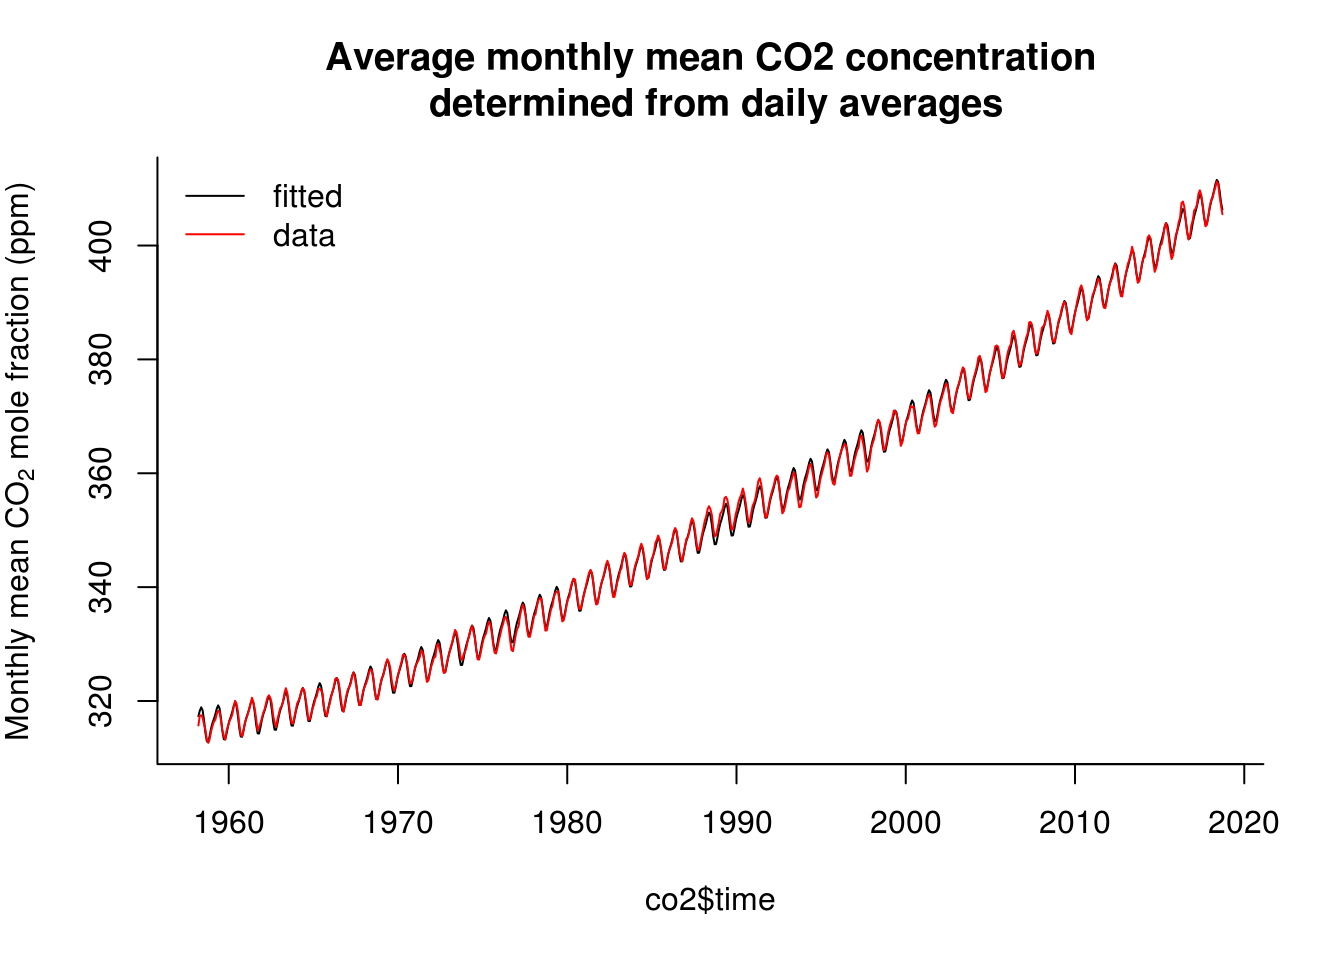
\includegraphics{timeseRies_files/figure-latex/Question_4-6.pdf}

\begin{Shaded}
\begin{Highlighting}[]
\CommentTok{# Trend not quite adequate because more exponential growth.  The trend does}
\CommentTok{# poorly in low-high observations Some discrepancy between the frequencies}
\CommentTok{# and the fitted Creates residual harmonic patterns - because trend minus}
\CommentTok{# fitted}
\NormalTok{res <-}\StringTok{ }\KeywordTok{residuals}\NormalTok{(lin_mod)}

\NormalTok{pairs.ts <-}\StringTok{ }\ControlFlowTok{function}\NormalTok{(d, }\DataTypeTok{lag.max =} \DecValTok{10}\NormalTok{) \{}
\NormalTok{    old_par <-}\StringTok{ }\KeywordTok{par}\NormalTok{(}\DataTypeTok{no.readonly =} \OtherTok{TRUE}\NormalTok{)}
\NormalTok{    n <-}\StringTok{ }\KeywordTok{length}\NormalTok{(d)}
\NormalTok{    X <-}\StringTok{ }\KeywordTok{matrix}\NormalTok{(}\OtherTok{NA}\NormalTok{, n }\OperatorTok{-}\StringTok{ }\NormalTok{lag.max, lag.max)}
\NormalTok{    col.names <-}\StringTok{ }\KeywordTok{paste}\NormalTok{(}\StringTok{"Time+"}\NormalTok{, }\DecValTok{1}\OperatorTok{:}\NormalTok{lag.max)}
    \ControlFlowTok{for}\NormalTok{ (i }\ControlFlowTok{in} \DecValTok{1}\OperatorTok{:}\NormalTok{lag.max) X[, i] <-}\StringTok{ }\NormalTok{d[i }\OperatorTok{-}\StringTok{ }\DecValTok{1} \OperatorTok{+}\StringTok{ }\DecValTok{1}\OperatorTok{:}\NormalTok{(n }\OperatorTok{-}\StringTok{ }\NormalTok{lag.max)]}
    \KeywordTok{par}\NormalTok{(}\DataTypeTok{mfrow =} \KeywordTok{c}\NormalTok{(}\DecValTok{3}\NormalTok{, }\DecValTok{3}\NormalTok{), }\DataTypeTok{pty =} \StringTok{"s"}\NormalTok{, }\DataTypeTok{mar =} \KeywordTok{c}\NormalTok{(}\DecValTok{3}\NormalTok{, }\DecValTok{4}\NormalTok{, }\FloatTok{0.5}\NormalTok{, }\FloatTok{0.5}\NormalTok{))}
\NormalTok{    lims <-}\StringTok{ }\KeywordTok{range}\NormalTok{(X)}
    \ControlFlowTok{for}\NormalTok{ (i }\ControlFlowTok{in} \DecValTok{2}\OperatorTok{:}\NormalTok{lag.max) }\KeywordTok{plot}\NormalTok{(X[, }\DecValTok{1}\NormalTok{], X[, i], }\DataTypeTok{panel.first =}\NormalTok{ \{}
        \KeywordTok{abline}\NormalTok{(}\DecValTok{0}\NormalTok{, }\DecValTok{1}\NormalTok{, }\DataTypeTok{col =} \StringTok{"grey"}\NormalTok{)}
\NormalTok{    \}, }\DataTypeTok{xlab =} \StringTok{"Time"}\NormalTok{, }\DataTypeTok{ylab =}\NormalTok{ col.names[i }\OperatorTok{-}\StringTok{ }\DecValTok{1}\NormalTok{], }\DataTypeTok{xlim =}\NormalTok{ lims, }\DataTypeTok{ylim =}\NormalTok{ lims, }\DataTypeTok{pch =} \DecValTok{20}\NormalTok{, }
        \DataTypeTok{col =} \KeywordTok{rgb}\NormalTok{(}\DecValTok{0}\NormalTok{, }\DecValTok{0}\NormalTok{, }\DecValTok{0}\NormalTok{, }\FloatTok{0.25}\NormalTok{))}
    \KeywordTok{par}\NormalTok{(old_par)}
\NormalTok{\}}
\KeywordTok{pairs.ts}\NormalTok{(res)}
\end{Highlighting}
\end{Shaded}

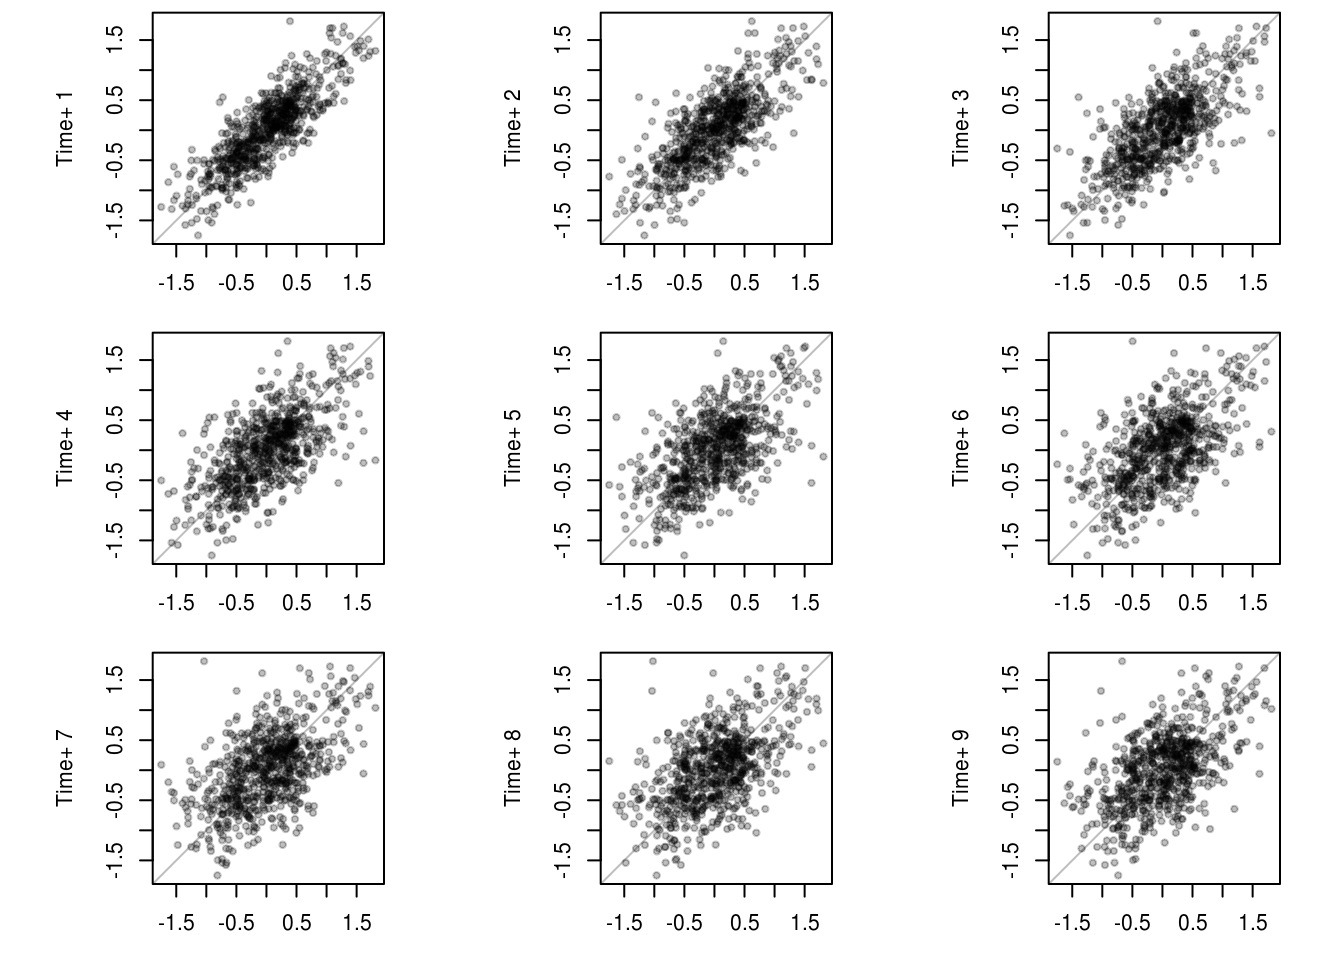
\includegraphics{timeseRies_files/figure-latex/Question_4-7.pdf}

\begin{Shaded}
\begin{Highlighting}[]
\KeywordTok{par}\NormalTok{(}\DataTypeTok{mfrow =} \KeywordTok{c}\NormalTok{(}\DecValTok{1}\NormalTok{, }\DecValTok{2}\NormalTok{))}
\NormalTok{TSA}\OperatorTok{::}\KeywordTok{acf}\NormalTok{(res, }\DataTypeTok{main =} \StringTok{"Residuals"}\NormalTok{)}
\KeywordTok{pacf}\NormalTok{(res, }\DataTypeTok{main =} \StringTok{"Residuals"}\NormalTok{)}
\end{Highlighting}
\end{Shaded}

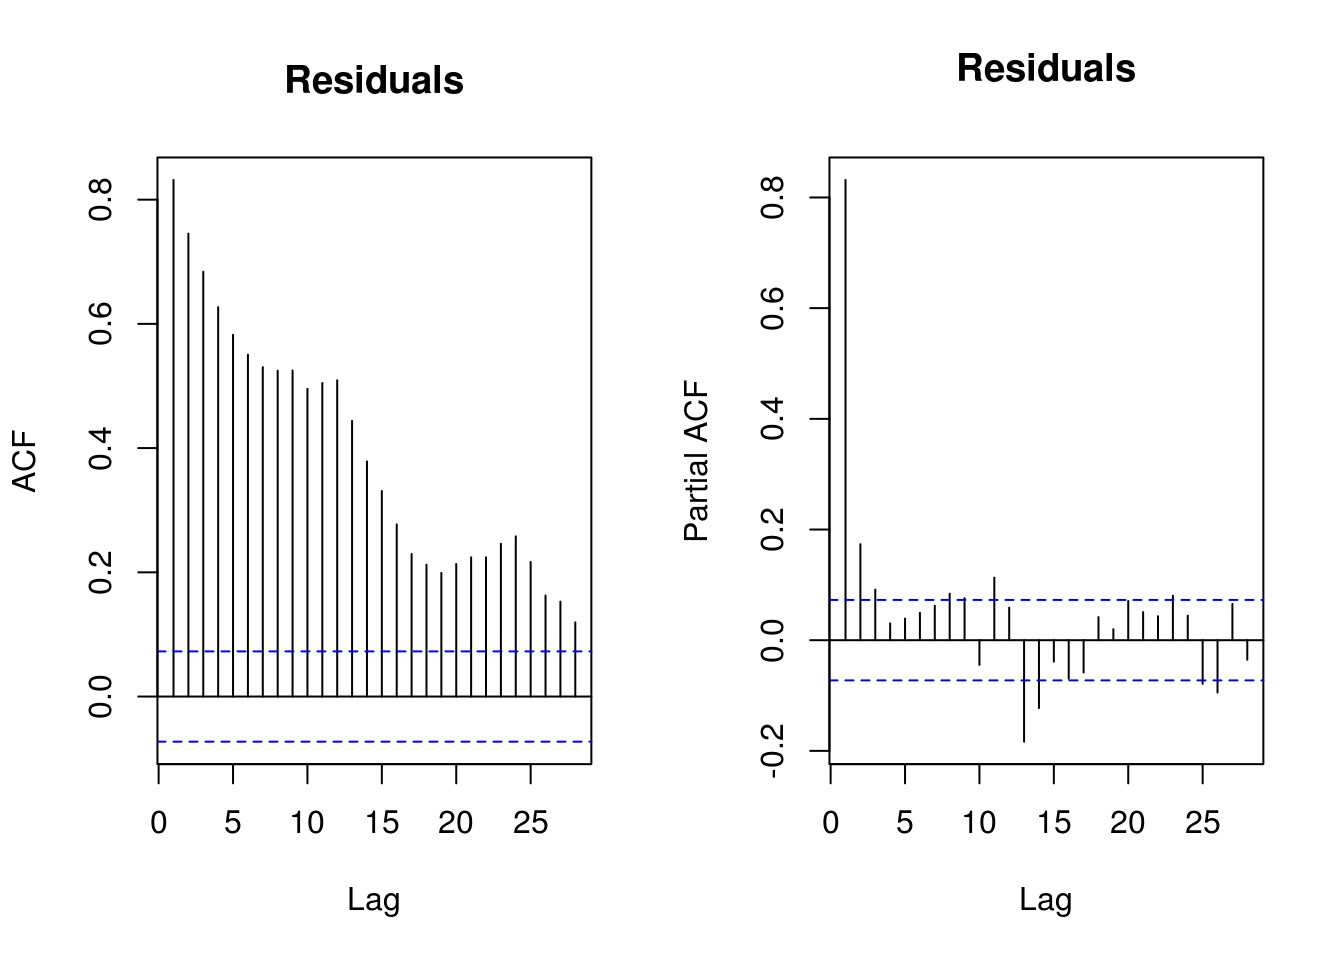
\includegraphics{timeseRies_files/figure-latex/Question_4-8.pdf}

\begin{Shaded}
\begin{Highlighting}[]
\KeywordTok{par}\NormalTok{(}\DataTypeTok{mfrow =} \KeywordTok{c}\NormalTok{(}\DecValTok{1}\NormalTok{, }\DecValTok{1}\NormalTok{))}
\CommentTok{# KS test: are residuals white noise?}
\KeywordTok{cpgram}\NormalTok{(res, }\DataTypeTok{main =} \StringTok{"Cumulative periodogram"}\NormalTok{)}
\end{Highlighting}
\end{Shaded}

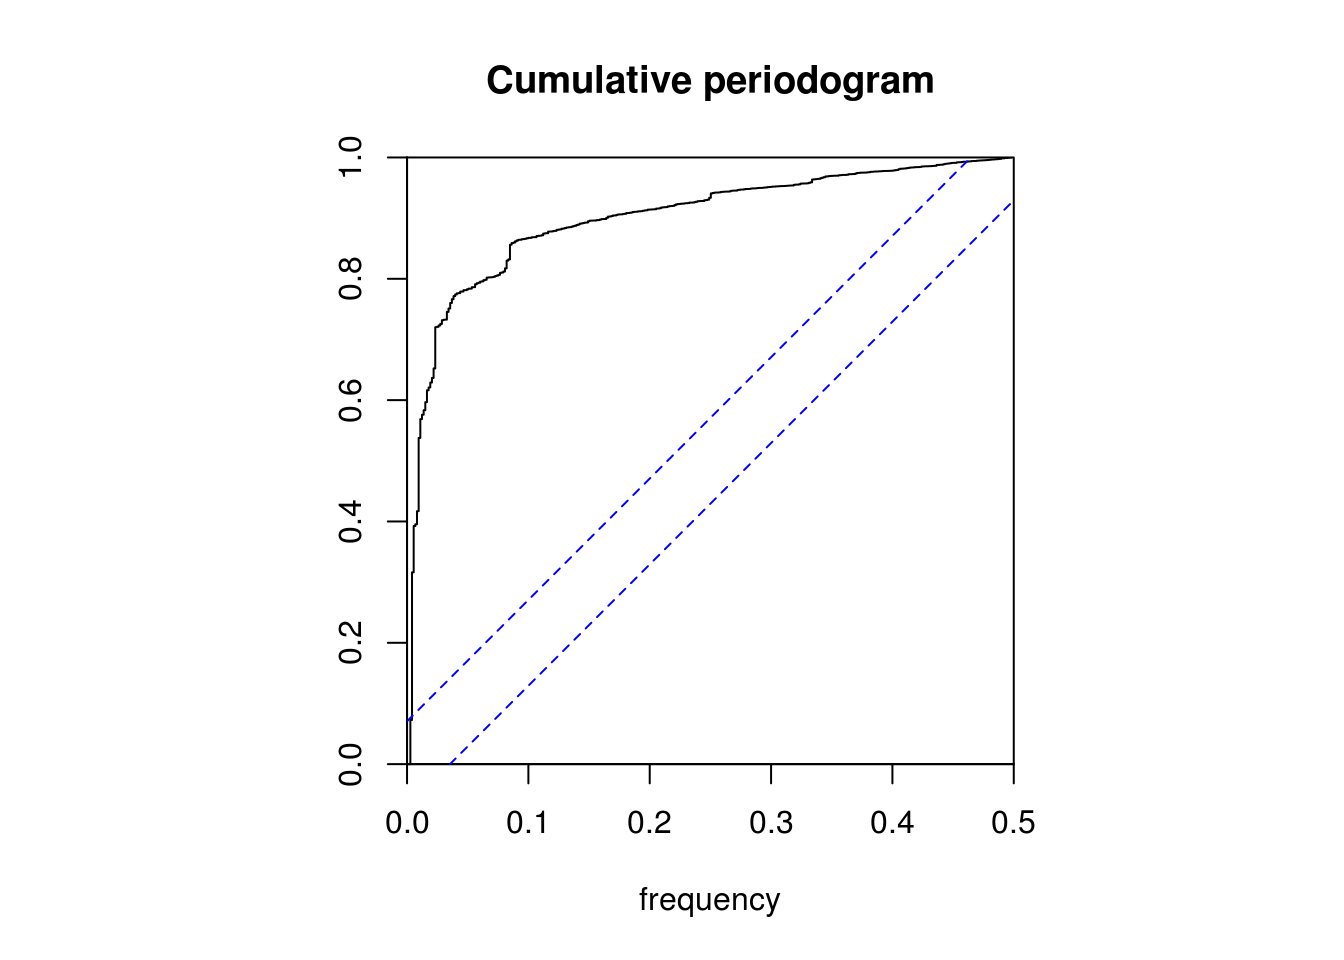
\includegraphics{timeseRies_files/figure-latex/Question_4-9.pdf}

\begin{Shaded}
\begin{Highlighting}[]
\CommentTok{# No, as one would expect}

\NormalTok{## Spectrum of raw series}
\KeywordTok{spectrum}\NormalTok{(co2}\OperatorTok{$}\NormalTok{interpolated)}
\end{Highlighting}
\end{Shaded}

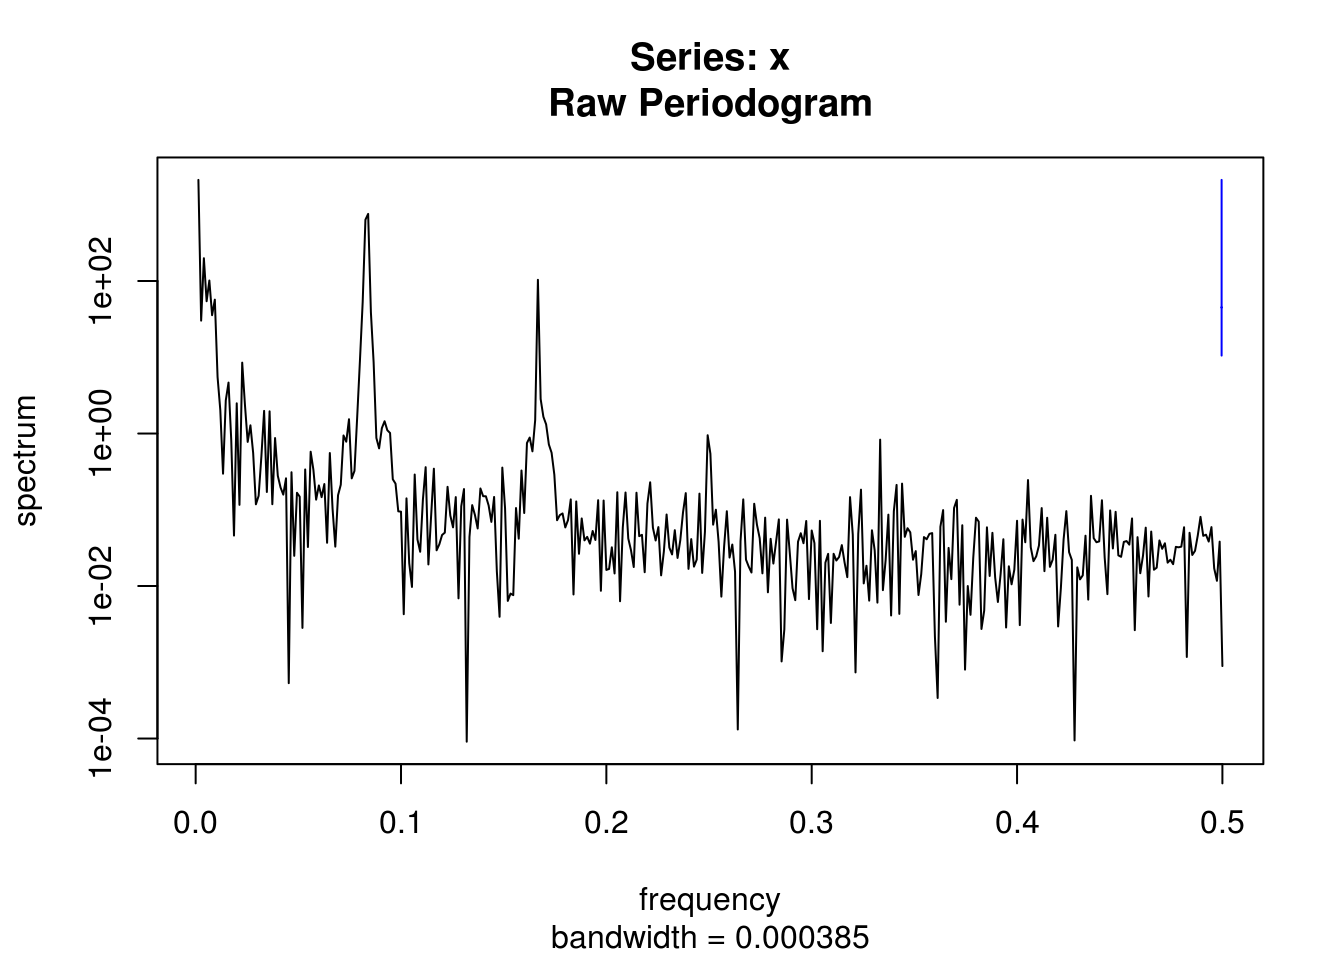
\includegraphics{timeseRies_files/figure-latex/Question_4-10.pdf}

\begin{Shaded}
\begin{Highlighting}[]
\CommentTok{# default with vector is to have frequency on [0,0.5]}
\KeywordTok{spectrum}\NormalTok{(co2_ts)  }\CommentTok{#otherwise corresponds to frequency of `ts`, here yearly}
\end{Highlighting}
\end{Shaded}

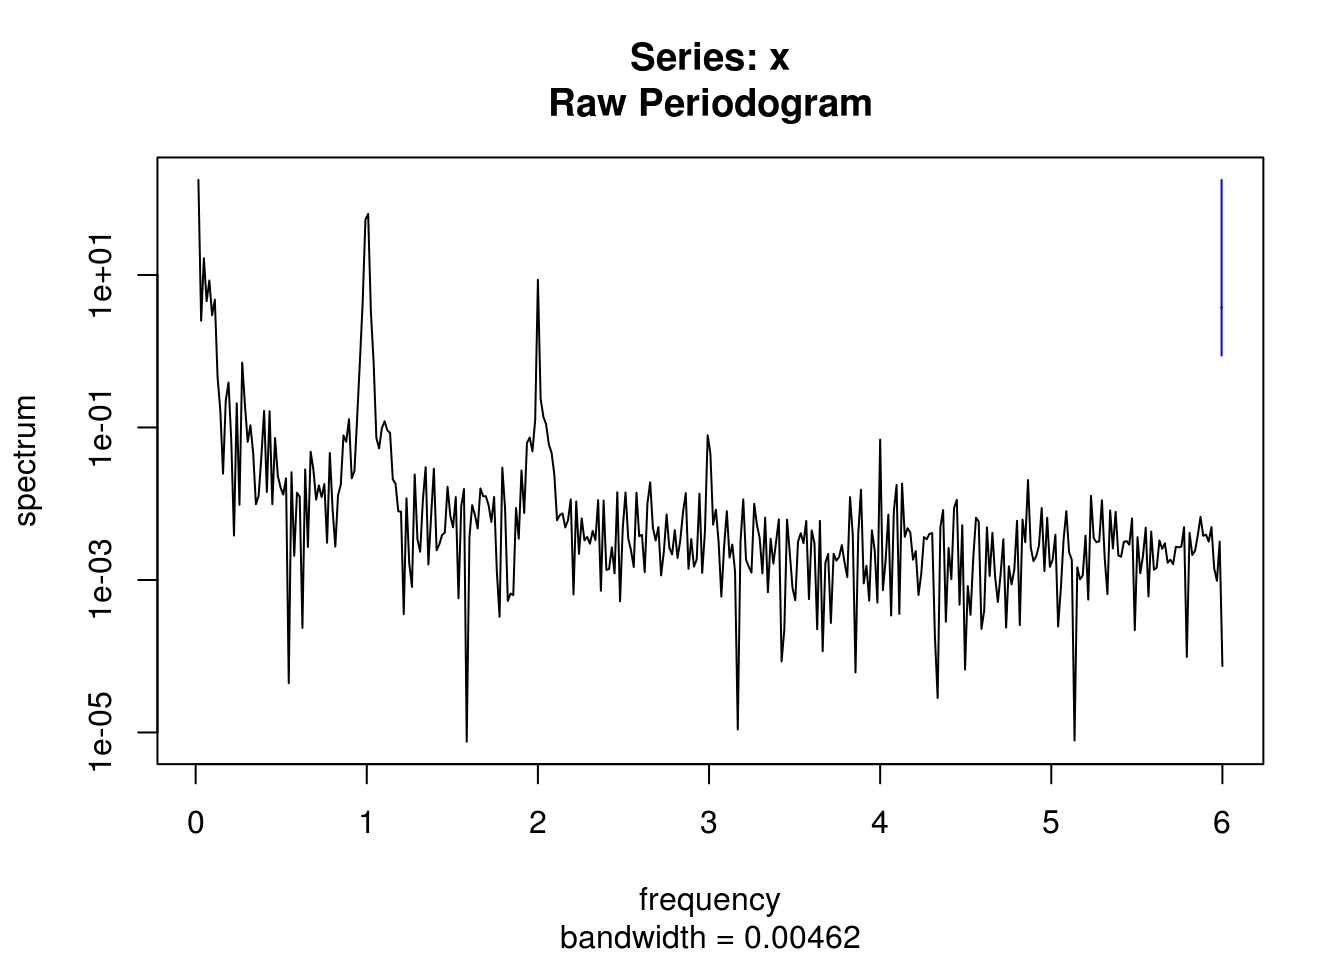
\includegraphics{timeseRies_files/figure-latex/Question_4-11.pdf}

\begin{Shaded}
\begin{Highlighting}[]
\NormalTok{filtered <-}\StringTok{ }\KeywordTok{filter}\NormalTok{(co2}\OperatorTok{$}\NormalTok{interpolated, }\DataTypeTok{method =} \StringTok{"convolution"}\NormalTok{, }\DataTypeTok{filter =} \KeywordTok{rep}\NormalTok{(}\DecValTok{1}\OperatorTok{/}\DecValTok{12}\NormalTok{, }
    \DecValTok{12}\NormalTok{))}
\KeywordTok{spectrum}\NormalTok{(}\KeywordTok{na.contiguous}\NormalTok{(filtered))}
\end{Highlighting}
\end{Shaded}

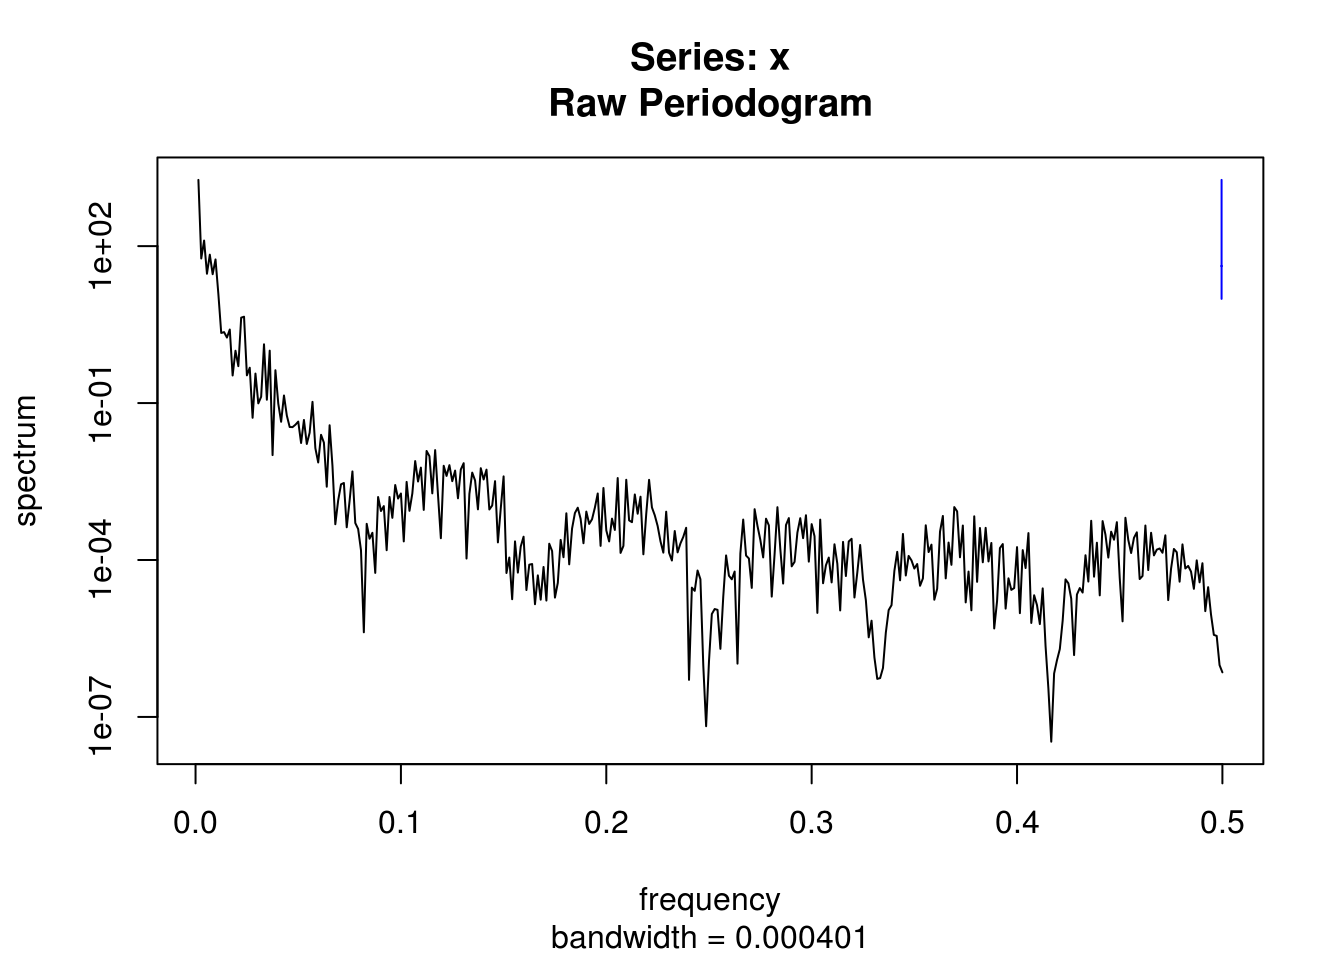
\includegraphics{timeseRies_files/figure-latex/Question_4-12.pdf}

\begin{Shaded}
\begin{Highlighting}[]
\CommentTok{# Detrended smoothed series}
\KeywordTok{spectrum}\NormalTok{(}\KeywordTok{resid}\NormalTok{(}\KeywordTok{lm}\NormalTok{(filtered }\OperatorTok{~}\StringTok{ }\KeywordTok{poly}\NormalTok{(co2}\OperatorTok{$}\NormalTok{time, }\DecValTok{2}\NormalTok{))))}
\end{Highlighting}
\end{Shaded}

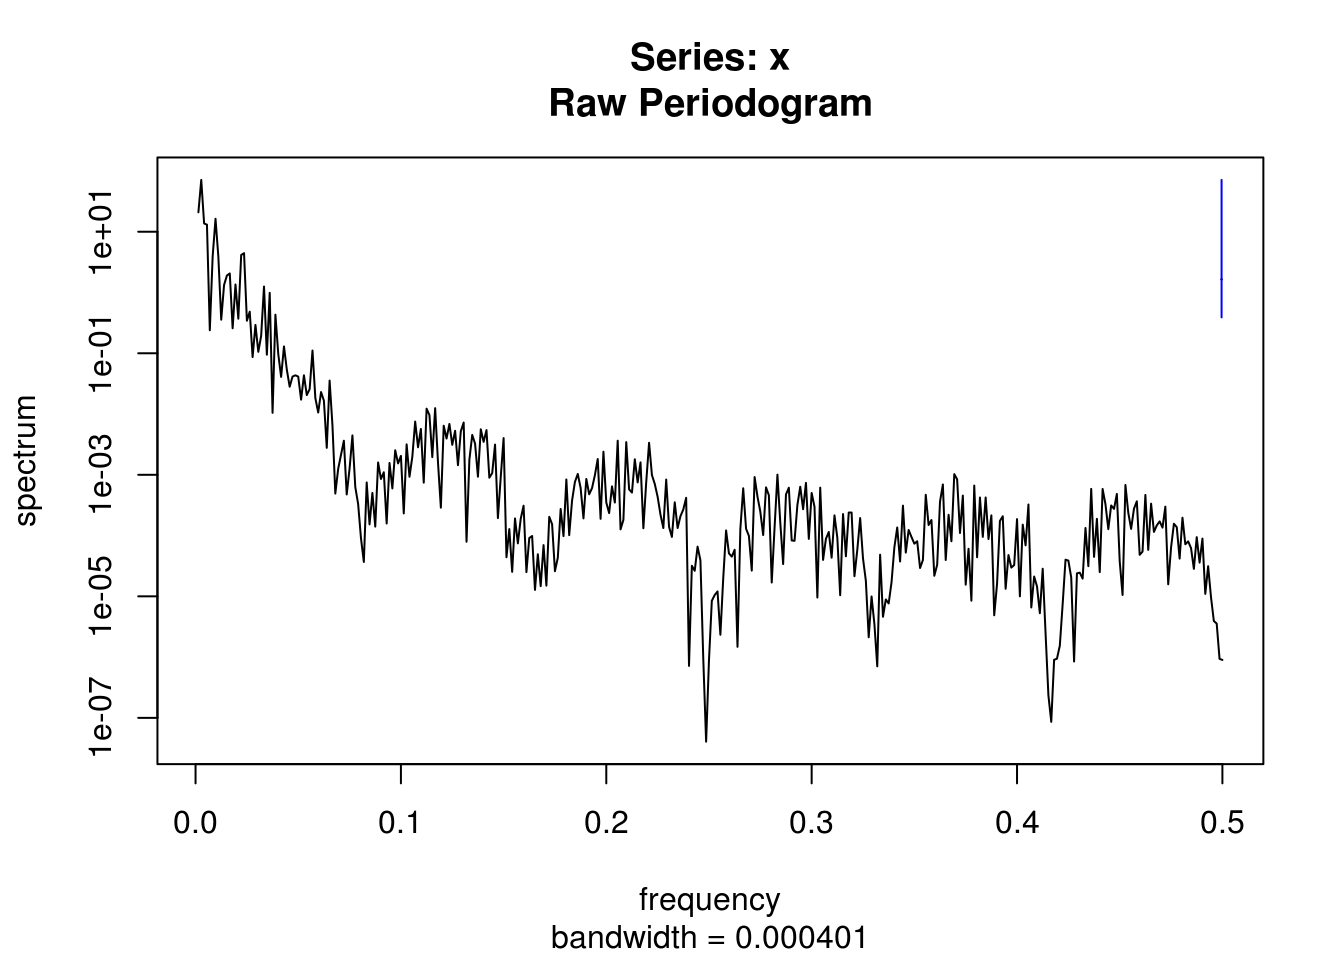
\includegraphics{timeseRies_files/figure-latex/Question_4-13.pdf}

\begin{Shaded}
\begin{Highlighting}[]
\CommentTok{# Test for H0}
\StringTok{`}\DataTypeTok{?}\StringTok{`}\NormalTok{(tseries}\OperatorTok{::}\NormalTok{kpss.test)}
\NormalTok{tseries}\OperatorTok{::}\KeywordTok{kpss.test}\NormalTok{(res, }\DataTypeTok{null =} \StringTok{"Level"}\NormalTok{)}
\end{Highlighting}
\end{Shaded}

\begin{verbatim}

    KPSS Test for Level Stationarity

data:  res
KPSS Level = 0.17017, Truncation lag parameter = 6, p-value = 0.1
\end{verbatim}

\begin{Shaded}
\begin{Highlighting}[]
\CommentTok{# Fail to reject null that it is level stationary}
\NormalTok{tseries}\OperatorTok{::}\KeywordTok{kpss.test}\NormalTok{(res, }\DataTypeTok{null =} \StringTok{"Trend"}\NormalTok{)}
\end{Highlighting}
\end{Shaded}

\begin{verbatim}

    KPSS Test for Trend Stationarity

data:  res
KPSS Trend = 0.17017, Truncation lag parameter = 6, p-value =
0.02986
\end{verbatim}

\begin{Shaded}
\begin{Highlighting}[]
\CommentTok{# Reject null at 5% that it is trend stationary}

\NormalTok{res_dec <-}\StringTok{ }\KeywordTok{decompose}\NormalTok{(co2_ts)}\OperatorTok{$}\NormalTok{random}
\NormalTok{res_stl <-}\StringTok{ }\KeywordTok{stl}\NormalTok{(co2_ts, }\DataTypeTok{s.window =} \StringTok{"periodic"}\NormalTok{)}\OperatorTok{$}\NormalTok{time.series[, }\StringTok{"remainder"}\NormalTok{]}

\KeywordTok{par}\NormalTok{(}\DataTypeTok{mfrow =} \KeywordTok{c}\NormalTok{(}\DecValTok{1}\NormalTok{, }\DecValTok{2}\NormalTok{))}
\CommentTok{# Some structure left due to incorrect model specification Residual}
\CommentTok{# frequency at lag 12-24 and two lag residuals}
\NormalTok{TSA}\OperatorTok{::}\KeywordTok{acf}\NormalTok{(res, }\DataTypeTok{na.action =}\NormalTok{ na.pass, }\DataTypeTok{main =} \StringTok{"Residuals from}\CharTok{\textbackslash{}n}\StringTok{ `lm`"}\NormalTok{)}
\KeywordTok{pacf}\NormalTok{(res, }\DataTypeTok{na.action =}\NormalTok{ na.pass, }\DataTypeTok{main =} \StringTok{"Residuals from}\CharTok{\textbackslash{}n}\StringTok{ `lm`"}\NormalTok{)}
\end{Highlighting}
\end{Shaded}

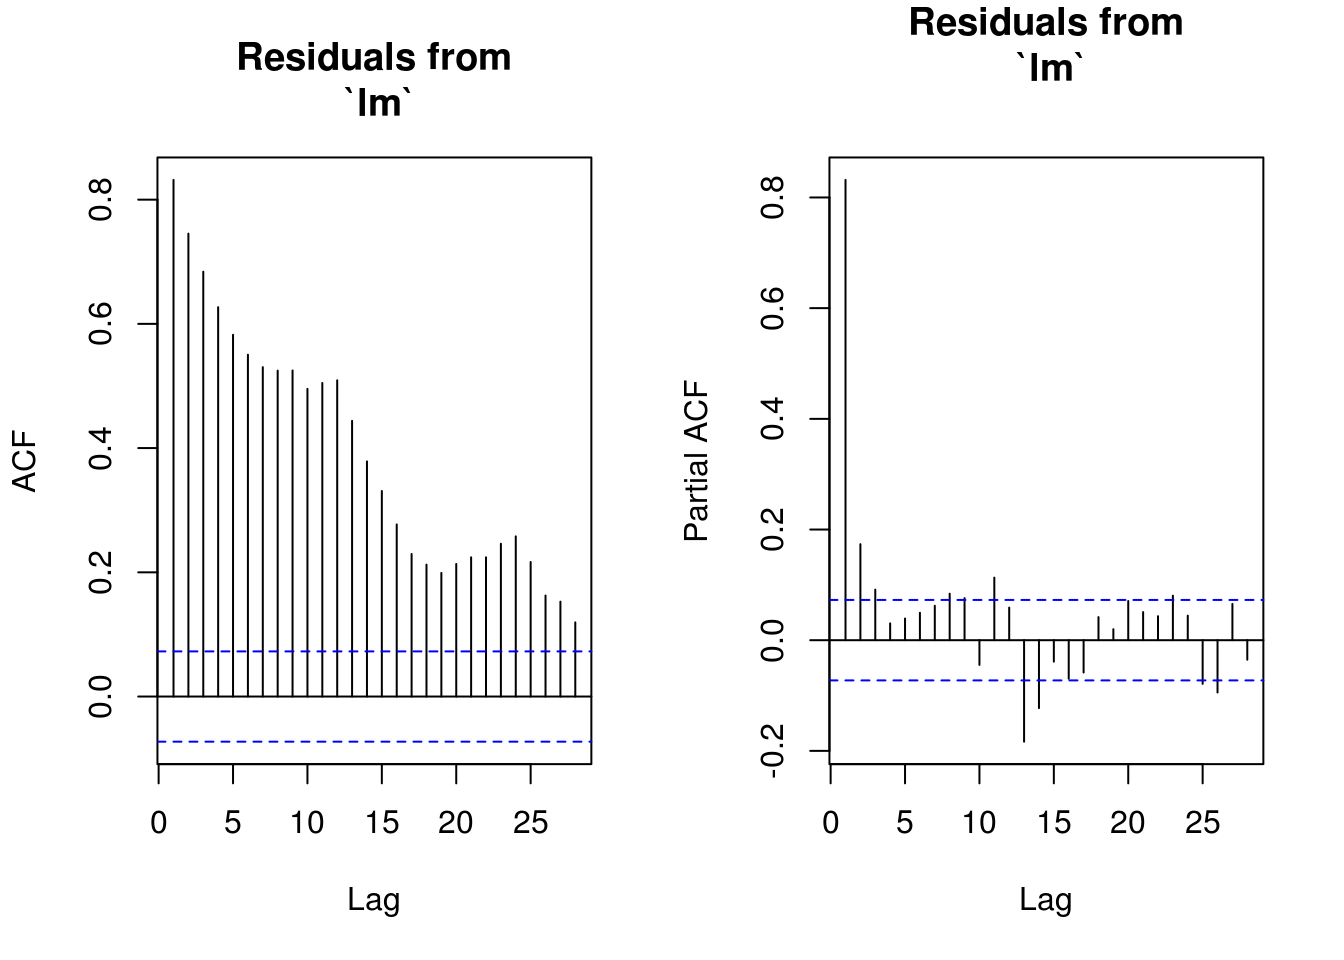
\includegraphics{timeseRies_files/figure-latex/Question_4-14.pdf}

\begin{Shaded}
\begin{Highlighting}[]
\CommentTok{# Residuals show some remaining periodicity at year 1. Would need AR(1)}
\CommentTok{# model}
\NormalTok{TSA}\OperatorTok{::}\KeywordTok{acf}\NormalTok{(res_dec, }\DataTypeTok{na.action =}\NormalTok{ na.pass, }\DataTypeTok{main =} \StringTok{"Residuals from}\CharTok{\textbackslash{}n}\StringTok{ `decompose`"}\NormalTok{)}
\KeywordTok{pacf}\NormalTok{(res_dec, }\DataTypeTok{na.action =}\NormalTok{ na.pass, }\DataTypeTok{main =} \StringTok{"Residuals from}\CharTok{\textbackslash{}n}\StringTok{ `decompose`"}\NormalTok{)}
\end{Highlighting}
\end{Shaded}

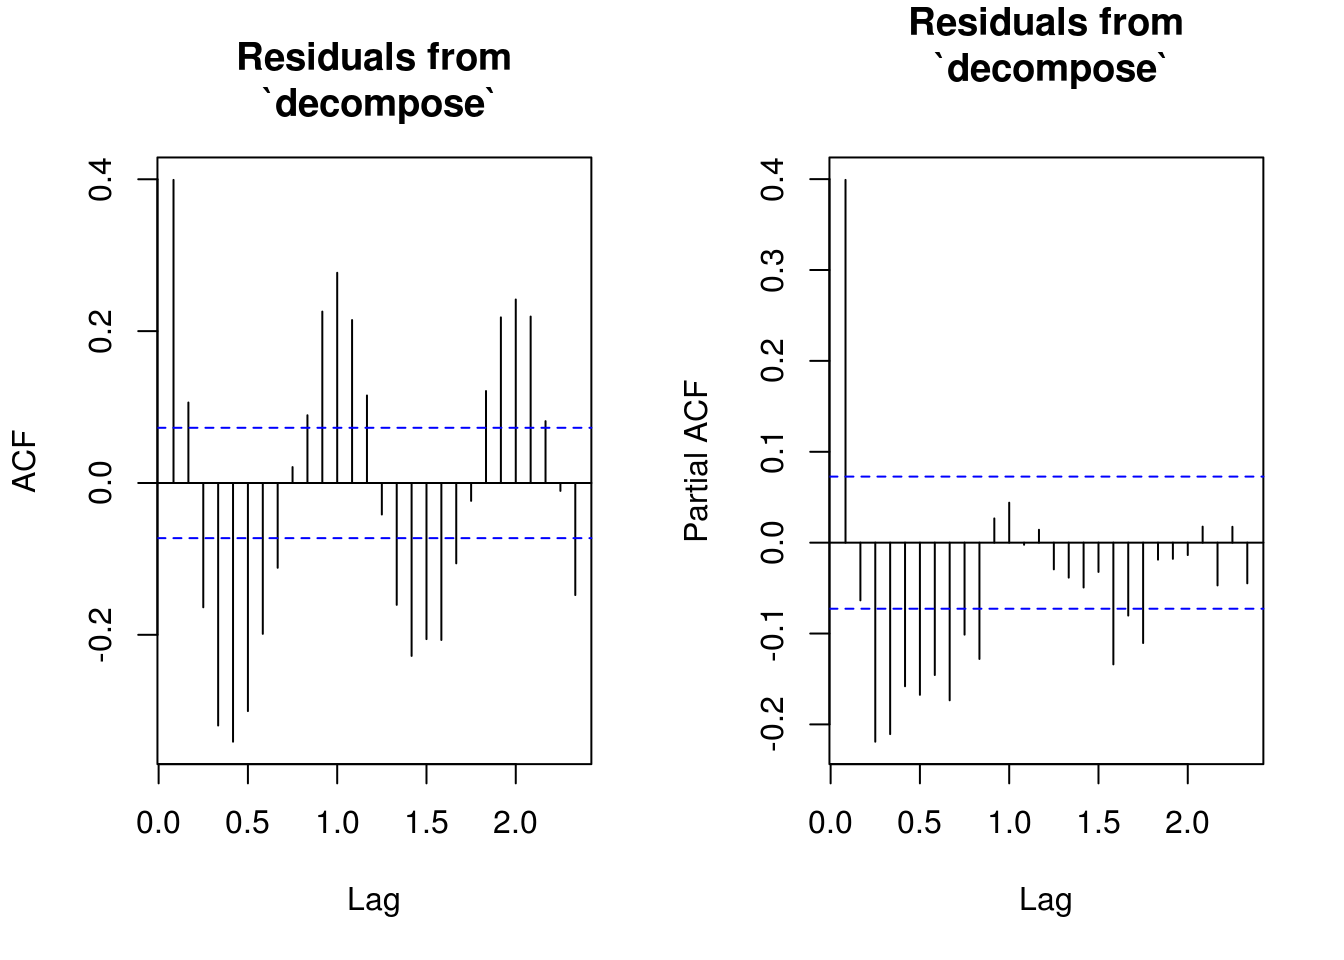
\includegraphics{timeseRies_files/figure-latex/Question_4-15.pdf}

\begin{Shaded}
\begin{Highlighting}[]
\CommentTok{# Similar output}
\NormalTok{TSA}\OperatorTok{::}\KeywordTok{acf}\NormalTok{(res_stl, }\DataTypeTok{main =} \StringTok{"Residuals from}\CharTok{\textbackslash{}n}\StringTok{ `stl`"}\NormalTok{)}
\KeywordTok{pacf}\NormalTok{(res_stl, }\DataTypeTok{main =} \StringTok{"Residuals from}\CharTok{\textbackslash{}n}\StringTok{ `stl`"}\NormalTok{)}
\end{Highlighting}
\end{Shaded}

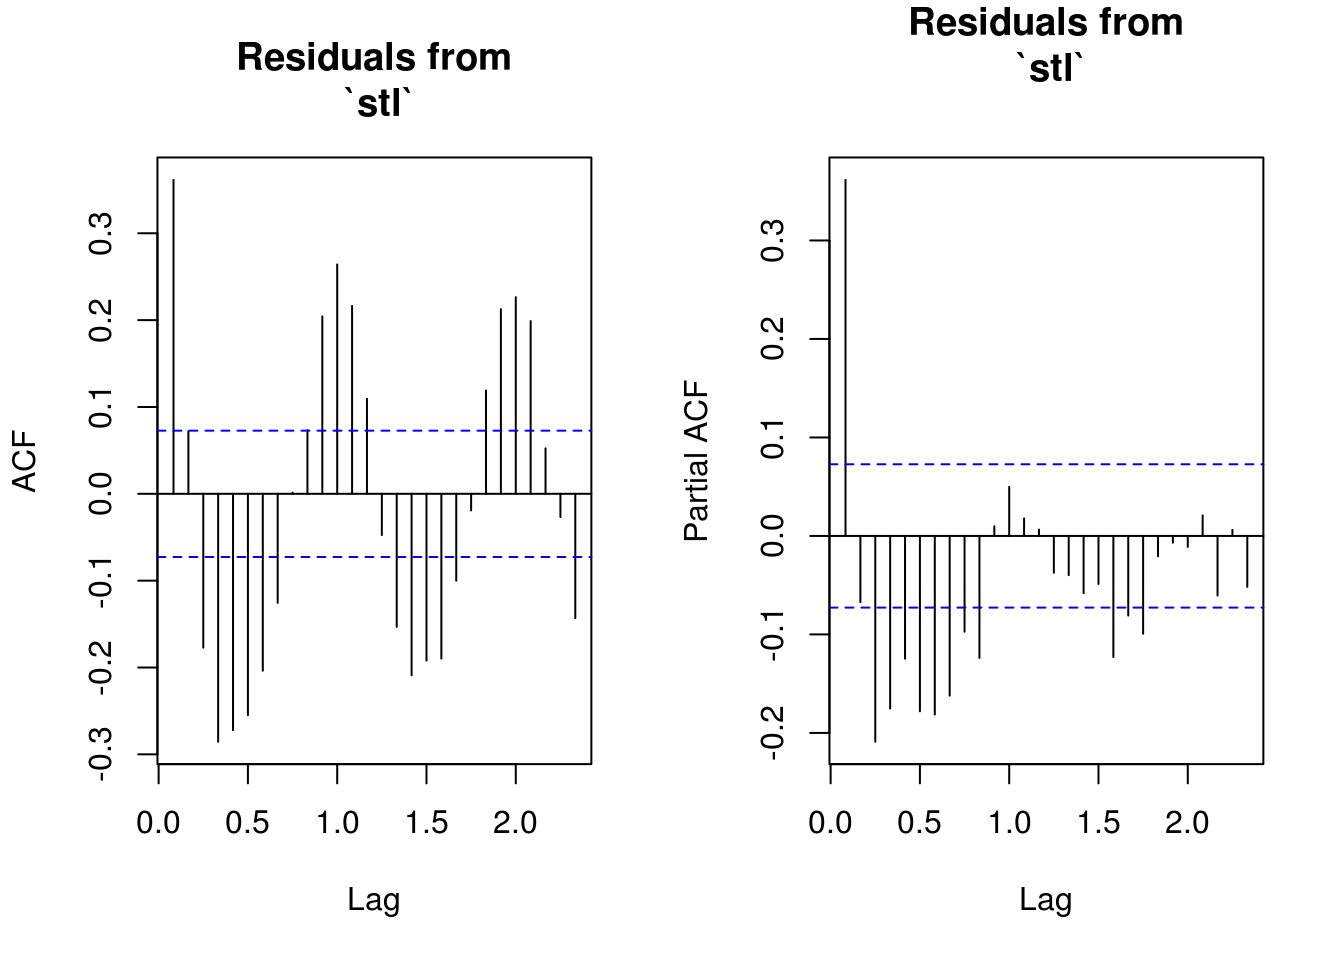
\includegraphics{timeseRies_files/figure-latex/Question_4-16.pdf}

\chapter{Likelihood estimation and the Box--Jenkins
method}\label{likelihood-estimation-and-the-boxjenkins-method}

This tutorial addresses the following:

\begin{itemize}
\tightlist
\item
  estimation of ARIMA and ARCH models using conditional maximum
  likelihood.
\item
  the Box--Jenkins methodology for selecting the order of ARMA processes
  based on analysis of the (partial) correlogram.
\item
  model selection using information criterion, unit roots and problems
  arising from model fit.
\end{itemize}

\section{Manual maximum likelihood
estimation}\label{manual-maximum-likelihood-estimation}

As was done in class for the \texttt{beaver} dataset, we will look at
manual specification of the likelihood. While it is straightforward in
principle to maximize the latter for ARMA models, the numerous
restrictions that are imposed on the parameters make it hard, if not
impossible, to manually code one's own function. Maximum likelihood
estimation is implemented typically via the state-space representation,
which we will cover later in the semester.

For simple models, it is easily done however, and should shed some light
on the various functions that are part of \textbf{R} for optimization,
the definition of a function, the use of \texttt{nlm} and \texttt{optim}
for optimization purposes, etc.

We first load a dataset of UBS and Credit Suisse stock prices from 2000
until 2008. The data is splitted in three parts for the analysis, since
the data is heteroscedastic, and there appears (visually) to be two
changepoints. We look at the adequacy of fitted AR(1) model for the mean
and an ARCH(1) for the variance.

\begin{Shaded}
\begin{Highlighting}[]
\CommentTok{# devtools::install_github('nickpoison/astsa')}
\CommentTok{# devtools::install_github('joshuaulrich/xts')}
\KeywordTok{library}\NormalTok{(xts)}
\KeywordTok{library}\NormalTok{(lubridate)}
\CommentTok{# read data and examine it}
\NormalTok{UBSCreditSuisse <-}\StringTok{ }\KeywordTok{read.csv}\NormalTok{(}\StringTok{"http://sma.epfl.ch/~lbelzile/math342/UBSCSG.csv"}\NormalTok{, }
    \DataTypeTok{stringsAsFactors =} \OtherTok{FALSE}\NormalTok{)}
\KeywordTok{names}\NormalTok{(UBSCreditSuisse)}
\end{Highlighting}
\end{Shaded}

\begin{verbatim}
 [1] "Date"       "UBS_OPEN"   "UBS_HIGH"   "UBS_LOW"    "UBS_LAST"  
 [6] "UBS_VOLUME" "CSG_OPEN"   "CSG_HIGH"   "CSG_LOW"    "CSG_LAST"  
[11] "CSG_VOLUME"
\end{verbatim}

\begin{Shaded}
\begin{Highlighting}[]
\KeywordTok{head}\NormalTok{(UBSCreditSuisse)}
\end{Highlighting}
\end{Shaded}

\begin{verbatim}
    Date UBS_OPEN UBS_HIGH UBS_LOW UBS_LAST UBS_VOLUME CSG_OPEN CSG_HIGH
1 1/1/00       NA       NA      NA       NA         NA       NA       NA
2 1/2/00       NA       NA      NA       NA         NA       NA       NA
3 1/3/00       NA       NA      NA       NA         NA       NA       NA
4 1/4/00    31.13    31.17   30.32    30.32   11526322    72.01    72.13
5 1/5/00    30.06    31.06   29.73    30.32   17142124    67.51    69.01
6 1/6/00    30.29    30.80   30.25    30.47    9509228    68.09    68.55
  CSG_LOW CSG_LAST CSG_VOLUME
1      NA       NA         NA
2      NA       NA         NA
3      NA       NA         NA
4   69.13    69.24    5336924
5   67.40    68.44    4419160
6   67.74    68.55    2585800
\end{verbatim}

\begin{Shaded}
\begin{Highlighting}[]
\CommentTok{# create time series, accounting for missing values at weekends and 251.25}
\CommentTok{# values/year this is correct for analysis, but only provides approximate}
\CommentTok{# locations for plotting}
\NormalTok{UBS <-}\StringTok{ }\KeywordTok{ts}\NormalTok{(UBSCreditSuisse}\OperatorTok{$}\NormalTok{UBS_LAST, }\DataTypeTok{start =} \KeywordTok{c}\NormalTok{(}\DecValTok{2000}\NormalTok{, }\DecValTok{1}\NormalTok{), }\DataTypeTok{frequency =} \FloatTok{365.25}\NormalTok{)}
\NormalTok{UBS <-}\StringTok{ }\KeywordTok{ts}\NormalTok{(UBS[}\OperatorTok{!}\KeywordTok{is.na}\NormalTok{(UBS)], }\DataTypeTok{start =} \KeywordTok{c}\NormalTok{(}\DecValTok{2000}\NormalTok{, }\DecValTok{1}\NormalTok{), }\DataTypeTok{frequency =} \FloatTok{251.625}\NormalTok{)}

\CommentTok{# Irregular time series}
\NormalTok{UBS_xts <-}\StringTok{ }\KeywordTok{with}\NormalTok{(UBSCreditSuisse, }\KeywordTok{xts}\NormalTok{(UBS_LAST, }\KeywordTok{mdy}\NormalTok{(Date)))}
\end{Highlighting}
\end{Shaded}

Objects of class \texttt{ts} store the dates from the vector start with
observations as \((i-1)/\omega\). Thus, we specified in the above a
vector encoded as 2000, 2000+1/365.25, \ldots This means that missing
values are not handled. In contrast, \texttt{xts} objects keep the time
stamps from a \texttt{Date} object. The function \texttt{with} is
equivalent to \texttt{attach}, but has a limited scope and is used to
avoid writing \texttt{UBSCreditSuisse\$Date}, etc. The function
\texttt{mdy} transforms the string \texttt{Date} as month, day and year.
The string is coerced into an object of class \texttt{Date}.

\begin{Shaded}
\begin{Highlighting}[]
\CommentTok{# Analysis for UBS returns, 2000-2008}
\NormalTok{UBS_ret <-}\StringTok{ }\DecValTok{100} \OperatorTok{*}\StringTok{ }\KeywordTok{diff}\NormalTok{(}\KeywordTok{log}\NormalTok{(UBS_xts))}
\KeywordTok{plot.zoo}\NormalTok{(UBS_ret, }\DataTypeTok{xlab =} \StringTok{"Time"}\NormalTok{, }\DataTypeTok{ylab =}\NormalTok{ (ylab <-}\StringTok{ "Daily returns (in %)"}\NormalTok{), }\DataTypeTok{main =} \StringTok{"Percentage daily growth rate of UBS stock"}\NormalTok{)}
\end{Highlighting}
\end{Shaded}

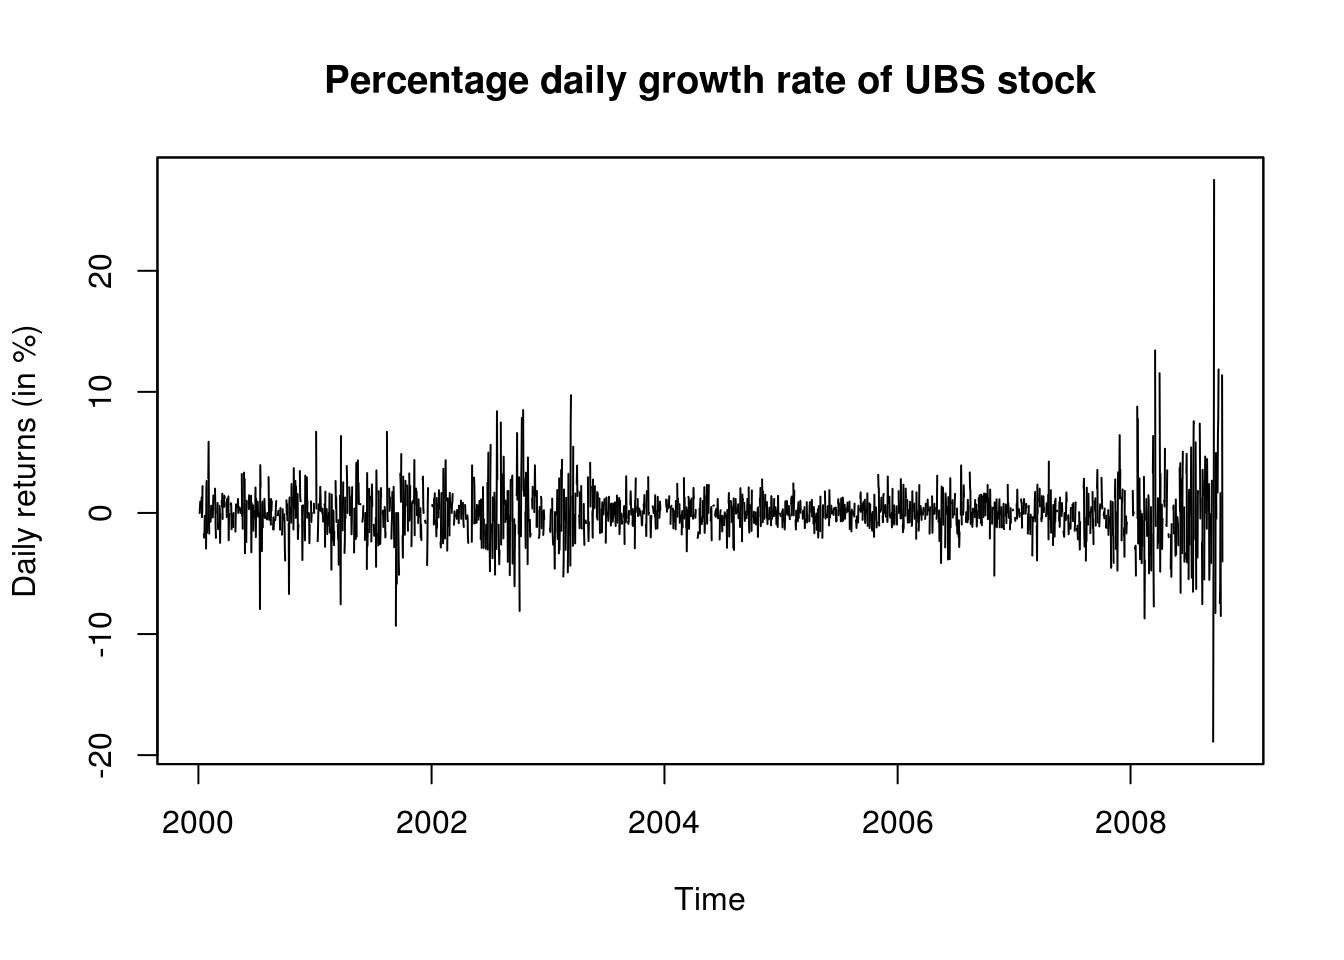
\includegraphics{timeseRies_files/figure-latex/unnamed-chunk-10-1.pdf}

\begin{Shaded}
\begin{Highlighting}[]
\CommentTok{# compute log returns}
\NormalTok{UBS.ret <-}\StringTok{ }\DecValTok{100} \OperatorTok{*}\StringTok{ }\KeywordTok{diff}\NormalTok{(}\KeywordTok{log}\NormalTok{(UBS))}

\CommentTok{# split into 3 homogeneous(?) parts, and plot using the same vertical axis}
\CommentTok{# on the graphs}

\CommentTok{# with the xts object}
\KeywordTok{par}\NormalTok{(}\DataTypeTok{mfrow =} \KeywordTok{c}\NormalTok{(}\DecValTok{1}\NormalTok{, }\DecValTok{3}\NormalTok{))}
\NormalTok{lims <-}\StringTok{ }\KeywordTok{range}\NormalTok{(UBS.ret)}
\KeywordTok{plot.zoo}\NormalTok{(UBS_ret[}\KeywordTok{paste0}\NormalTok{(}\KeywordTok{index}\NormalTok{(}\KeywordTok{first}\NormalTok{(UBS_ret)), }\StringTok{"/"}\NormalTok{, }\KeywordTok{as.Date}\NormalTok{(}\StringTok{"2003-01-01"}\NormalTok{) }\OperatorTok{+}\StringTok{ }
\StringTok{    }\DecValTok{100}\NormalTok{)], }\DataTypeTok{ylim =}\NormalTok{ lims, }\DataTypeTok{xlab =} \StringTok{"Time"}\NormalTok{, }\DataTypeTok{ylab =}\NormalTok{ ylab)}

\CommentTok{# with window and the ts object}
\NormalTok{y1 <-}\StringTok{ }\KeywordTok{window}\NormalTok{(UBS.ret, }\DataTypeTok{end =} \KeywordTok{c}\NormalTok{(}\DecValTok{2003}\NormalTok{, }\DecValTok{100}\NormalTok{))}
\CommentTok{# plot(y1, ylim = lims)}

\NormalTok{y2 <-}\StringTok{ }\KeywordTok{window}\NormalTok{(UBS.ret, }\DataTypeTok{start =} \KeywordTok{c}\NormalTok{(}\DecValTok{2003}\NormalTok{, }\DecValTok{101}\NormalTok{), }\DataTypeTok{end =} \KeywordTok{c}\NormalTok{(}\DecValTok{2007}\NormalTok{, }\DecValTok{200}\NormalTok{))}
\KeywordTok{plot}\NormalTok{(y2, }\DataTypeTok{ylim =}\NormalTok{ lims, }\DataTypeTok{ylab =}\NormalTok{ ylab, }\DataTypeTok{main =} \StringTok{"UBS daily growth rate (in %)"}\NormalTok{)}

\NormalTok{y3 <-}\StringTok{ }\KeywordTok{window}\NormalTok{(UBS.ret, }\DataTypeTok{start =} \KeywordTok{c}\NormalTok{(}\DecValTok{2007}\NormalTok{, }\DecValTok{201}\NormalTok{))}
\KeywordTok{plot}\NormalTok{(y3, }\DataTypeTok{ylim =}\NormalTok{ lims, }\DataTypeTok{ylab =}\NormalTok{ ylab)}
\end{Highlighting}
\end{Shaded}

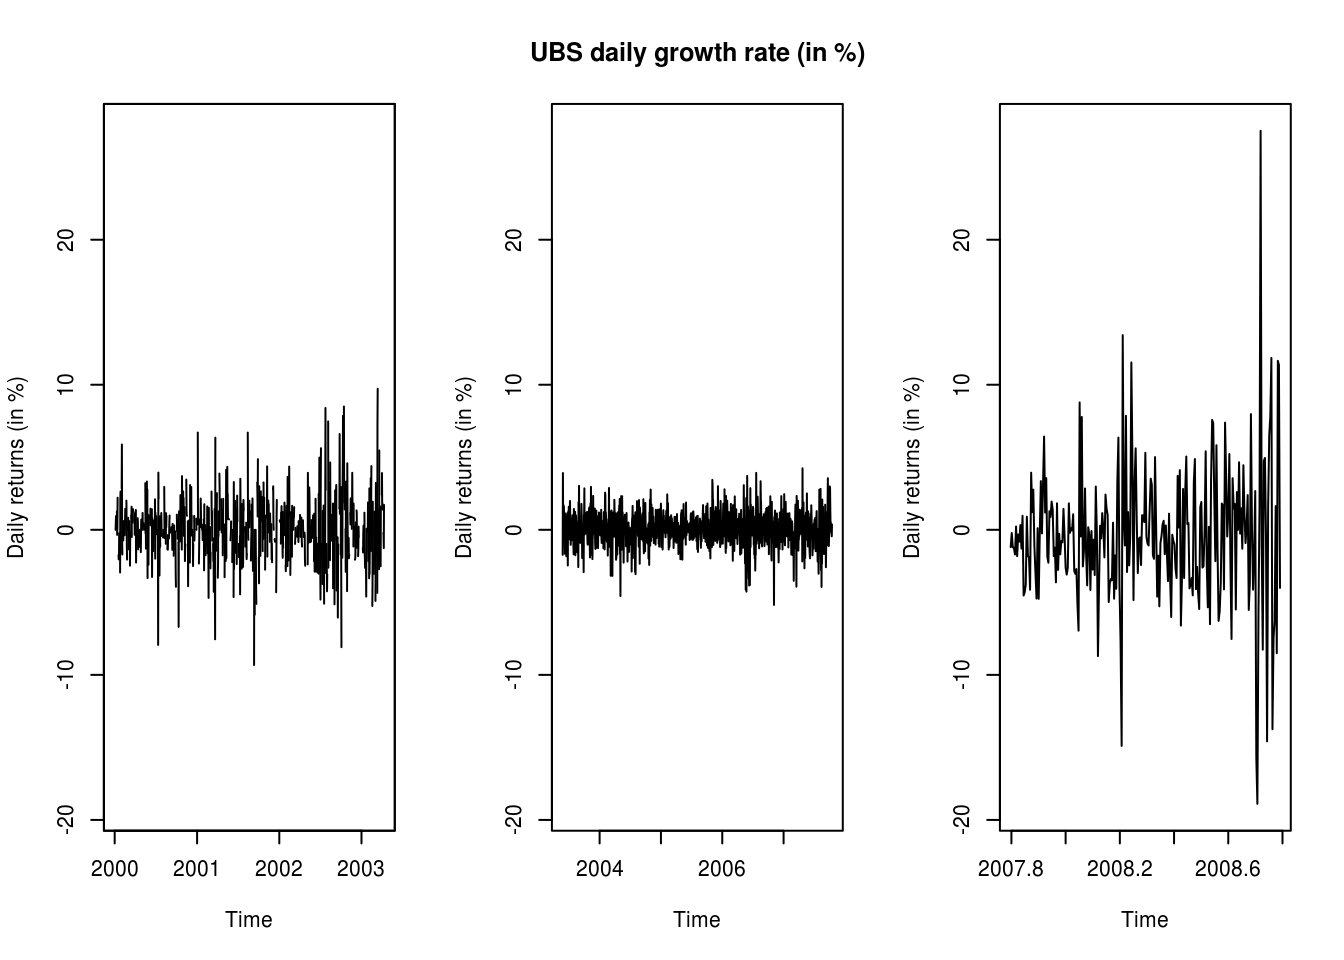
\includegraphics{timeseRies_files/figure-latex/unnamed-chunk-10-2.pdf}

\begin{Shaded}
\begin{Highlighting}[]
\CommentTok{# analysis of first part, first just plotting ACF and PACF for data and for}
\CommentTok{# abs(data)}
\NormalTok{y <-}\StringTok{ }\NormalTok{y1}

\CommentTok{# (Partial) correlograms for the series}
\KeywordTok{par}\NormalTok{(}\DataTypeTok{mfrow =} \KeywordTok{c}\NormalTok{(}\DecValTok{2}\NormalTok{, }\DecValTok{2}\NormalTok{))}
\NormalTok{TSA}\OperatorTok{::}\KeywordTok{acf}\NormalTok{(y, }\DataTypeTok{lag.max =} \DecValTok{100}\NormalTok{, }\DataTypeTok{main =} \StringTok{"Daily log returns (%)"}\NormalTok{)}
\KeywordTok{pacf}\NormalTok{(y, }\DataTypeTok{lag.max =} \DecValTok{100}\NormalTok{, , }\DataTypeTok{main =} \StringTok{""}\NormalTok{)}
\NormalTok{TSA}\OperatorTok{::}\KeywordTok{acf}\NormalTok{(}\KeywordTok{abs}\NormalTok{(y), }\DataTypeTok{lag.max =} \DecValTok{100}\NormalTok{, }\DataTypeTok{main =} \StringTok{"Absolute daily log returns (%)"}\NormalTok{)}
\KeywordTok{pacf}\NormalTok{(}\KeywordTok{abs}\NormalTok{(y), }\DataTypeTok{lag.max =} \DecValTok{100}\NormalTok{, }\DataTypeTok{main =} \StringTok{""}\NormalTok{)}
\end{Highlighting}
\end{Shaded}

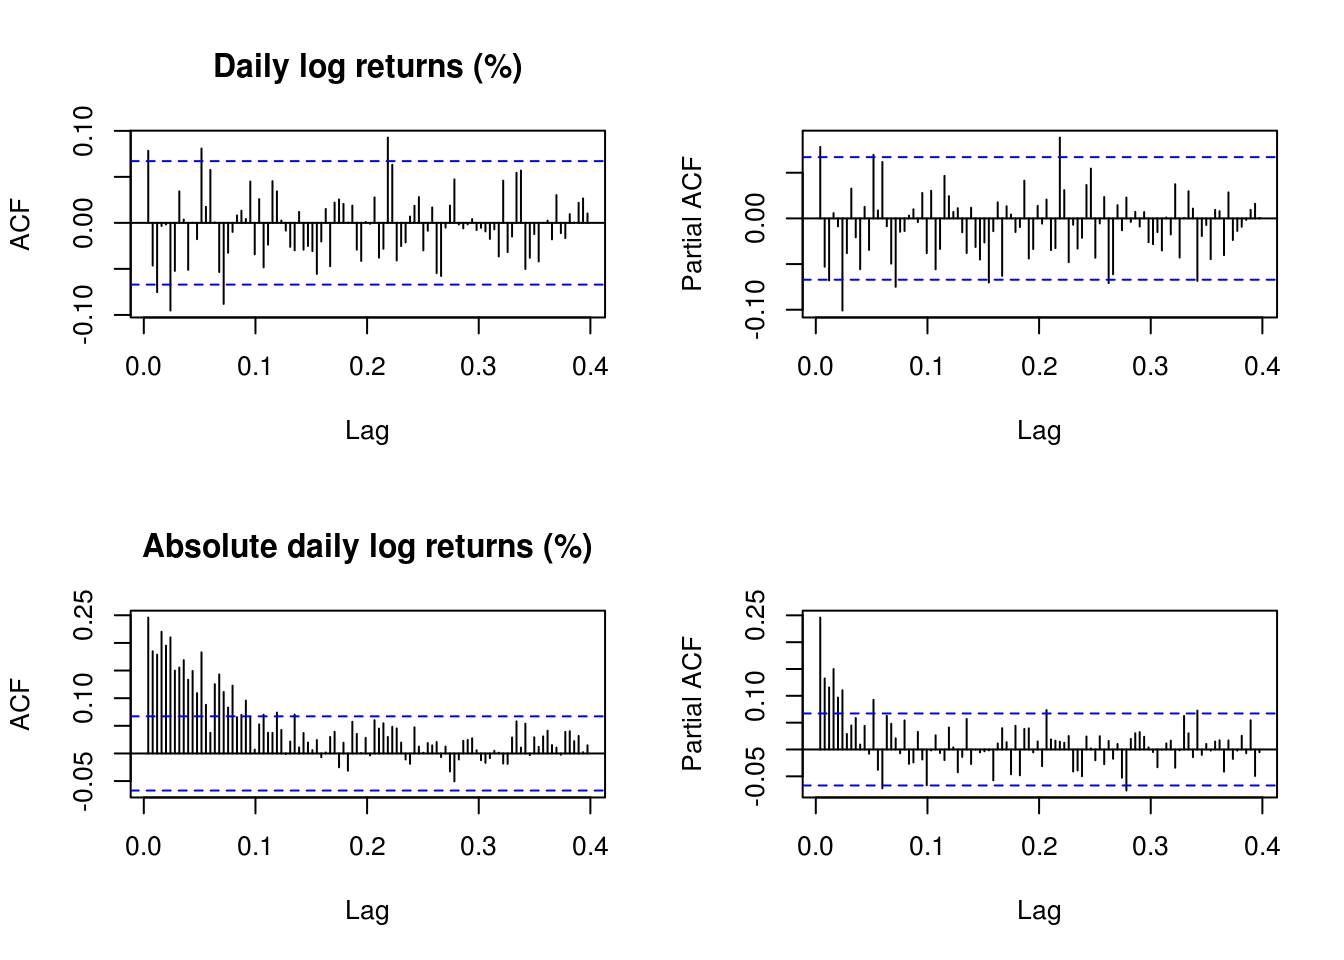
\includegraphics{timeseRies_files/figure-latex/unnamed-chunk-10-3.pdf}

The residuals look pretty much white noise, but the variance has
residual structure. Recall the implicit definition of the AR(1) process
\(Y_t\), \[Y_t=\mu+\phi(Y_{t-1}-\mu)+\varepsilon_t,\] where
\(\varepsilon_t \stackrel{\mathrm{iid}}{\sim} \mathcal{N}(0,\sigma^2)\).
The joint distribution of the observations conditional on the first is
multivariate normal. Here is a simple function for the likelihood, which
only requires specifying the conditional mean.

\begin{Shaded}
\begin{Highlighting}[]
\CommentTok{# analysis using AR(1) model for means conditional likelihood}
\NormalTok{nll_AR1 <-}\StringTok{ }\ControlFlowTok{function}\NormalTok{(th, y) \{}
\NormalTok{    n <-}\StringTok{ }\KeywordTok{length}\NormalTok{(y)}
\NormalTok{    condit.mean <-}\StringTok{ }\NormalTok{th[}\DecValTok{1}\NormalTok{] }\OperatorTok{+}\StringTok{ }\NormalTok{th[}\DecValTok{3}\NormalTok{] }\OperatorTok{*}\StringTok{ }\NormalTok{(y[}\OperatorTok{-}\NormalTok{n] }\OperatorTok{-}\StringTok{ }\NormalTok{th[}\DecValTok{1}\NormalTok{])}
    \OperatorTok{-}\KeywordTok{sum}\NormalTok{(}\KeywordTok{dnorm}\NormalTok{(y[}\OperatorTok{-}\DecValTok{1}\NormalTok{], }\DataTypeTok{mean =}\NormalTok{ condit.mean, }\DataTypeTok{sd =}\NormalTok{ th[}\DecValTok{2}\NormalTok{], }\DataTypeTok{log =} \OtherTok{TRUE}\NormalTok{))}
\NormalTok{\}}
\NormalTok{init1 <-}\StringTok{ }\KeywordTok{c}\NormalTok{(}\DecValTok{0}\NormalTok{, }\DecValTok{1}\NormalTok{, }\FloatTok{0.5}\NormalTok{)}
\CommentTok{# fit1 <- nlm(f = nll_AR1, p = init1, iterlim = 500, hessian = TRUE, y = y)}
\NormalTok{fit1 <-}\StringTok{ }\KeywordTok{optim}\NormalTok{(init1, nll_AR1, }\DataTypeTok{y =}\NormalTok{ y, }\DataTypeTok{hessian =} \OtherTok{TRUE}\NormalTok{, }\DataTypeTok{method =} \StringTok{"Nelder-Mead"}\NormalTok{)}
\end{Highlighting}
\end{Shaded}

We obtain the parameter estimates and the standard errors from the
observed information matrix, estimated numerically. Incidently, one can
easily that the problem is equivalent to a linear Gaussian model where
the regressor is a lagged vector of observations. The parameter
estimates differ slightly, but this is due to the optimization routine.

\begin{verbatim}
#Parameter values (MLEs)
fit1$par
#Standard errors from inverse of Hessian matrix at MLE
#If you code the optimization routine yourself, you can still obtain the Hessian via
#hessian <- numDeriv::hessian(func = nll_AR1, y = y, x = fit1$par)

#Standard errors
sqrt(diag(solve(fit1$hessian)))

#Conditional likelihood using lm 
#dynlm is a wrapper around lm for `ts` and `zoo` objects, L means lag and you can add e.g. trend(y)
fit1_ols <- dynlm::dynlm(y ~ L(y, 1))
coefficients(fit1_ols)
sd(residuals(fit1_ols))
\end{verbatim}

Incidently, the situation is analogous for the ARCH(1) process, which
has a conditional variance that changes over time. The latter is defined
implicitly as \[
\begin{align*}
Z_t &= \mu + \sigma_t\epsilon_t\\
\sigma_t^2 &=\alpha_0+\alpha_1(Z_{t-1}-\mu)^2 
\end{align*}
\] with \(\epsilon_t \stackrel{\mathrm{iid}}{\sim} \mathcal{N}(0, 1)\).

The variance \(\sigma^2\) here is included as \(\sigma^2=\alpha_0\) and
the parameter appearing in the likelihood is \(\alpha_1/\sigma^2\)
corresponds to \(\theta_3\), or \texttt{th{[}3{]}}.

\begin{Shaded}
\begin{Highlighting}[]
\CommentTok{# analysis using ARCH(1) model for variances}
\NormalTok{nll_ARCH1 <-}\StringTok{ }\ControlFlowTok{function}\NormalTok{(th, y) \{}
\NormalTok{    n <-}\StringTok{ }\KeywordTok{length}\NormalTok{(y)}
\NormalTok{    condit.mean <-}\StringTok{ }\NormalTok{th[}\DecValTok{1}\NormalTok{]}
\NormalTok{    condit.var <-}\StringTok{ }\NormalTok{th[}\DecValTok{2}\NormalTok{] }\OperatorTok{*}\StringTok{ }\NormalTok{(}\DecValTok{1} \OperatorTok{+}\StringTok{ }\NormalTok{th[}\DecValTok{3}\NormalTok{] }\OperatorTok{*}\StringTok{ }\NormalTok{(y[}\OperatorTok{-}\NormalTok{n] }\OperatorTok{-}\StringTok{ }\NormalTok{th[}\DecValTok{1}\NormalTok{])}\OperatorTok{^}\DecValTok{2}\NormalTok{)}
    \OperatorTok{-}\KeywordTok{sum}\NormalTok{(}\KeywordTok{dnorm}\NormalTok{(y[}\OperatorTok{-}\DecValTok{1}\NormalTok{], }\DataTypeTok{mean =}\NormalTok{ condit.mean, }\DataTypeTok{sd =} \KeywordTok{sqrt}\NormalTok{(condit.var), }\DataTypeTok{log =} \OtherTok{TRUE}\NormalTok{))}
\NormalTok{\}}
\NormalTok{init2 <-}\StringTok{ }\KeywordTok{c}\NormalTok{(}\DecValTok{0}\NormalTok{, }\DecValTok{1}\NormalTok{, }\FloatTok{0.5}\NormalTok{)}
\NormalTok{fit2 <-}\StringTok{ }\KeywordTok{nlm}\NormalTok{(}\DataTypeTok{f =}\NormalTok{ nll_ARCH1, }\DataTypeTok{p =}\NormalTok{ init2, }\DataTypeTok{iterlim =} \DecValTok{500}\NormalTok{, }\DataTypeTok{hessian =} \OtherTok{TRUE}\NormalTok{, }\DataTypeTok{y =}\NormalTok{ y)}
\NormalTok{## fit2 <- optim(init2, nll_ARCH1, y = y, hessian = TRUE)}
\end{Highlighting}
\end{Shaded}

The function \texttt{nlm} performs minimization, but may return warnings
because some of its steps because the conditional variance can be
negative for some combinations of the variable, so the corresponding
moves of the Newton algorithm are rejected. These are typically steps
that are not in the neighborhood of the final solution, so can be
ignored if the output is valid. The \texttt{minimum} corresponds to the
negative log-likelihood at the maximum likelihood estimates. The MLE is
given by \texttt{estimate} and the standard errors by the square root of
the diagonal entries of the inverse Hessian (here already negated
because we work with the negative of the log-likelihood). Since the
residuals have a varying variance, we need to adjust them by dividing
each by their respective variance. Same would have occured for the AR(1)
process, but it is easier for the mean.

\begin{Shaded}
\begin{Highlighting}[]
\NormalTok{fit2}\OperatorTok{$}\NormalTok{minimum}
\end{Highlighting}
\end{Shaded}

\begin{verbatim}
[1] 1860.386
\end{verbatim}

\begin{Shaded}
\begin{Highlighting}[]
\NormalTok{fit2}\OperatorTok{$}\NormalTok{estimate}
\end{Highlighting}
\end{Shaded}

\begin{verbatim}
[1] 0.02691498 3.31180313 0.11770094
\end{verbatim}

\begin{Shaded}
\begin{Highlighting}[]
\KeywordTok{sqrt}\NormalTok{(}\KeywordTok{diag}\NormalTok{(}\KeywordTok{solve}\NormalTok{(fit2}\OperatorTok{$}\NormalTok{hessian)))}
\end{Highlighting}
\end{Shaded}

\begin{verbatim}
[1] 0.06843004 0.24664944 0.02908274
\end{verbatim}

\begin{Shaded}
\begin{Highlighting}[]
\NormalTok{make_resid_ARCH1 <-}\StringTok{ }\ControlFlowTok{function}\NormalTok{(y, fit) \{}
\NormalTok{    th <-}\StringTok{ }\NormalTok{fit}\OperatorTok{$}\NormalTok{estimate}
\NormalTok{    n <-}\StringTok{ }\KeywordTok{length}\NormalTok{(y)}
\NormalTok{    condit.mean <-}\StringTok{ }\NormalTok{th[}\DecValTok{1}\NormalTok{]}
\NormalTok{    condit.var <-}\StringTok{ }\NormalTok{th[}\DecValTok{2}\NormalTok{] }\OperatorTok{*}\StringTok{ }\NormalTok{(}\DecValTok{1} \OperatorTok{+}\StringTok{ }\NormalTok{th[}\DecValTok{3}\NormalTok{] }\OperatorTok{*}\StringTok{ }\NormalTok{(y[}\OperatorTok{-}\NormalTok{n] }\OperatorTok{-}\StringTok{ }\NormalTok{th[}\DecValTok{1}\NormalTok{])}\OperatorTok{^}\DecValTok{2}\NormalTok{)}
\NormalTok{    res <-}\StringTok{ }\NormalTok{(y[}\OperatorTok{-}\DecValTok{1}\NormalTok{] }\OperatorTok{-}\StringTok{ }\NormalTok{condit.mean)}\OperatorTok{/}\KeywordTok{sqrt}\NormalTok{(condit.var)}
    \KeywordTok{ts}\NormalTok{(res)}
\NormalTok{\}}

\NormalTok{res2 <-}\StringTok{ }\KeywordTok{make_resid_ARCH1}\NormalTok{(y, fit2)}
\end{Highlighting}
\end{Shaded}

We now proceed with diagnostic plots to check the model adequacy. Recall
that the Kolmogorov--Smirnov test statistic associated with the
cumulative periodogram tests the hypothesis of white noise (and ARCH(1)
is white noise).

\begin{Shaded}
\begin{Highlighting}[]
\KeywordTok{par}\NormalTok{(}\DataTypeTok{mfrow =} \KeywordTok{c}\NormalTok{(}\DecValTok{2}\NormalTok{, }\DecValTok{2}\NormalTok{))}
\KeywordTok{plot}\NormalTok{(y, }\DataTypeTok{main =} \StringTok{"Raw returns"}\NormalTok{)}
\KeywordTok{plot}\NormalTok{(res2, }\DataTypeTok{main =} \StringTok{"ARCH(1) residuals"}\NormalTok{)}
\KeywordTok{cpgram}\NormalTok{(res2, }\DataTypeTok{main =} \StringTok{"Cumulative periodogram"}\NormalTok{)}
\KeywordTok{par}\NormalTok{(}\DataTypeTok{pty =} \StringTok{"s"}\NormalTok{)}
\KeywordTok{qqnorm}\NormalTok{(res2, }\DataTypeTok{panel.first =}\NormalTok{ \{}
    \KeywordTok{abline}\NormalTok{(}\DecValTok{0}\NormalTok{, }\DecValTok{1}\NormalTok{, }\DataTypeTok{col =} \StringTok{"red"}\NormalTok{)}
\NormalTok{\})}
\end{Highlighting}
\end{Shaded}

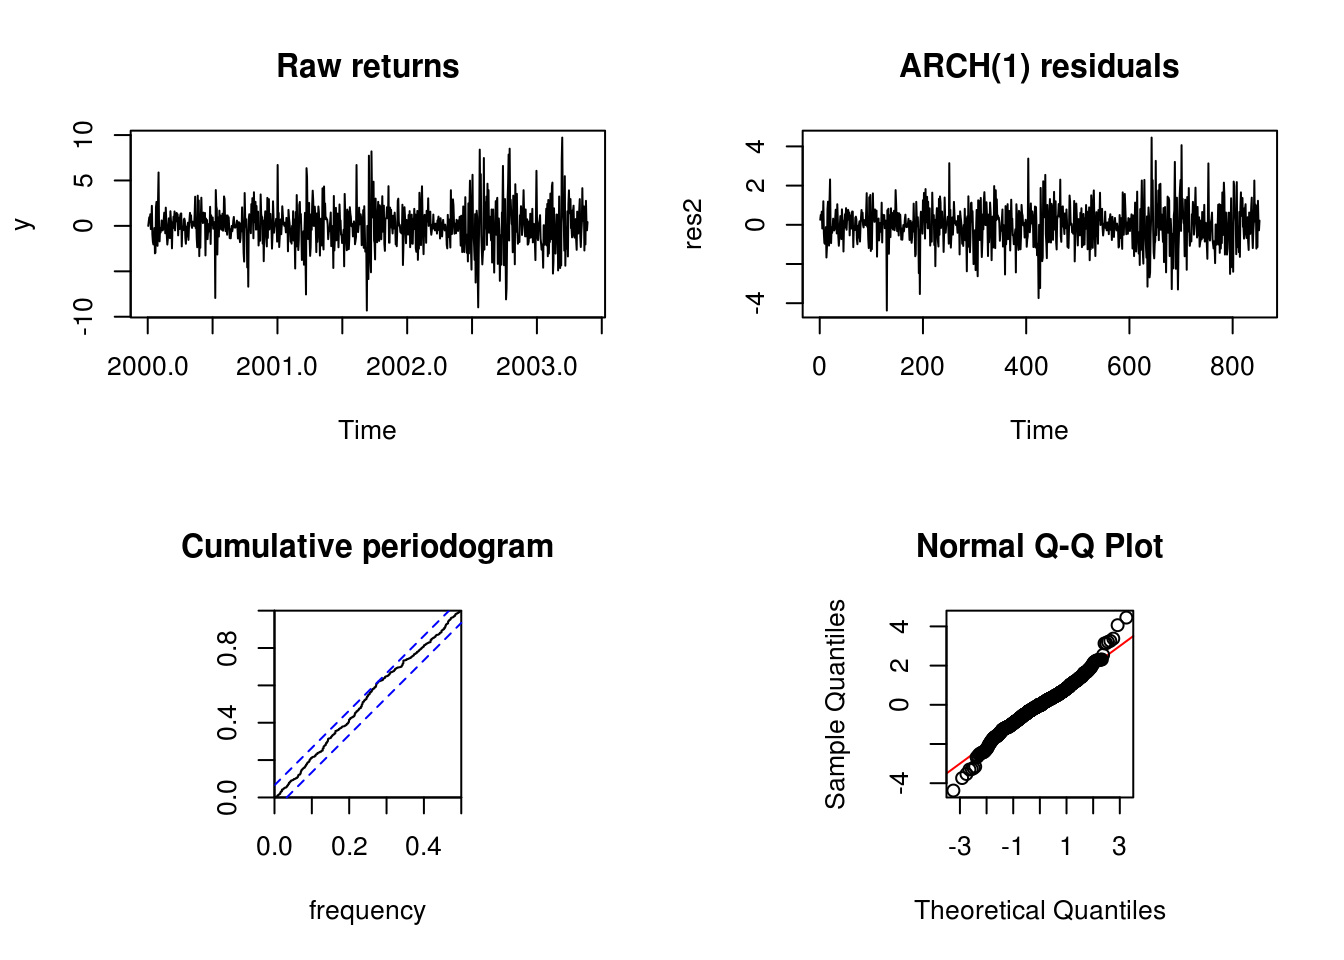
\includegraphics{timeseRies_files/figure-latex/diagnostics_ARCH-1.pdf}

\subsection{Exercise 1: UBS stock
returns}\label{exercise-1-ubs-stock-returns}

\begin{enumerate}
\def\labelenumi{\arabic{enumi}.}
\tightlist
\item
  Create a function that fits an AR(1)-ARCH(1) model by modifying the
  code provided above and apply it to \texttt{y}. The latter is defined
  as
  \[Y_t-\mu = \phi(Y_{t-1}-\mu)+\sigma_t\varepsilon_t, \quad \sigma^2_t = \alpha_0+\alpha_1(Y_{t-1}-\mu)^2, \quad \varepsilon_t \stackrel{\mathrm{iid}}{\sim} \mathcal{N}(0,\sigma^2)\]
\item
  Obtain the maximum likelihood estimates using \texttt{nlm} or
  \texttt{optim} as well as the standard errors
\item
  Plot the residuals. Comment on the fit using standard diagnostic plots
  (Q-Q plot, ((P)ACF, cumulative periodogram).
\item
  Fit an AR(2) model using a conditional likelihood for the mean and
  obtain the standard errors of your estimated coefficients.
\item
  Perform a likelihood ratio test to test whether the AR(2) coefficient
  is significative.
\end{enumerate}

\section{Box--Jenkins methodology for ARMA
models}\label{boxjenkins-methodology-for-arma-models}

The Wold decomposition theorem states that any second-order stationary
time series can be represented as a deterministic process and a
stochastic linear process, which can be represented as a causal
MA(\(\infty\)) series of the form
\[Y_t = \sum_{j = 0}^\infty \psi_j\varepsilon_{t-j}, \qquad \varepsilon_t \sim \mathrm{WN}(0, \sigma^2),\quad \psi_0 = 1, \quad\sum_{j = 0}^\infty \psi_j^2 < \infty\]

This does provide a justification for using an ARMA model for modelling.
The latter may not be parsimonious nor useful at characterizing the data
generating mechanism, but they nevertheless provide in some simple cases
a good approximation.

The Box--Jenkins methodology for ARMA models (dating back to time where
computing ressources were scarce) allows one to select the order of an
AR(\(p\)), MA(\(q\)) or ARMA(\(p, q\)) by visual inspection of the
(partial) correlograms. Both should always go alongside one another.

\begin{enumerate}
\def\labelenumi{\arabic{enumi}.}
\tightlist
\item
  Apply a transformation of the data \(X_t\) where appropriate
\end{enumerate}

\begin{itemize}
\tightlist
\item
  logarithm, Box--Cox transform
\item
  differencing so that the series appears linear.
\end{itemize}

\begin{enumerate}
\def\labelenumi{\arabic{enumi}.}
\setcounter{enumi}{1}
\tightlist
\item
  Correlogram
\end{enumerate}

\begin{itemize}
\tightlist
\item
  Determine the MA(\(q\)) order by looking at the autocorrelation, at
  the points for which \(\rho_k \neq 0\) for \(k \leq q\) and
  \(r_k \approx 0\) for \(k>q\).
\item
  For an AR(\(p\)) process, the autocorrelation function should decay
  exponentially, with possible oscillation patterns.
\item
  For an ARMA(\(p, q\)) model, the pattern is irregular for lags
  \(k = 1, \ldots, p\) and go to zero as \(k \to \infty\).
\end{itemize}

\begin{enumerate}
\def\labelenumi{\arabic{enumi}.}
\setcounter{enumi}{2}
\tightlist
\item
  Partial correlogram
\end{enumerate}

\begin{itemize}
\tightlist
\item
  Parameters should be zero at lags \(k>p\) for the AR(\(p\)) model, and
  nonzero otherwise
\item
  The parameters decay exponentially in the MA(\(q\)) model
\item
  The parameters decrease to zero as \(k \to \infty\) for the
  ARMA(\(p, q\)) model.
\end{itemize}

The function to fit these models is \texttt{arima}, whose arguments are
specified via \texttt{order\ =\ c(p,\ d,\ q)}. Ignore the \texttt{d}
component for now in the triple \((p, d, q)\) by setting it to zero.
Other options are \texttt{sarima} from \texttt{astsa}, which is a
wrapper around \texttt{arima}. \texttt{sarima} provides diagnostic plots
alongside and includes a constant by default, but the syntax differs
from \texttt{arima} and it takes directly components \(p\), \(d\) and
\(q\). The function \texttt{Arima} from Hyndman's \texttt{forecast}
package is yet another wrapper around \texttt{arima}. An explanation of
the differences can be found in
\href{https://www.otexts.org/fpp/8/7}{Forecasting: principles and
practice}, at the bottom of the page.

\begin{quote}
The \texttt{Arima()} command from the \texttt{forecast} package provides
more flexibility on the inclusion of a constant
\end{quote}

It also correctly labels the latter. Depending on your model, it may be
the level (mean), an intercept, the linear trend (slope, or drift in the
time serie literature). If we take first difference, the constant is the
drift, etc.

\textbf{Warning}: You may stumble on the web on \texttt{auto.arima.}
Beware of the naive and automated selection implemented by this function
(which relies on what I would consider to be an \emph{ad hoc} forward
model selection). Use at your own risk.

ARMA models can be almost equivalent, as the following example from
Shumway and Stoffer (example 3.28) illustrates. Note that as we use
\texttt{sarima}, a constant is included by default. We can assess its
significance by the usual \(t\)-test, if the error structure is
appropriate.

\begin{Shaded}
\begin{Highlighting}[]
\KeywordTok{library}\NormalTok{(astsa)}
\NormalTok{gnpgr =}\StringTok{ }\KeywordTok{diff}\NormalTok{(}\KeywordTok{log}\NormalTok{(gnp))  }\CommentTok{# growth rate of GNP}
\NormalTok{main <-}\StringTok{ "Quarterly growth rate}\CharTok{\textbackslash{}n}\StringTok{ of U.S. GNP"}
\KeywordTok{plot}\NormalTok{(gnpgr, }\DataTypeTok{main =}\NormalTok{ main, }\DataTypeTok{ylab =} \StringTok{"Growth rate"}\NormalTok{)}
\end{Highlighting}
\end{Shaded}

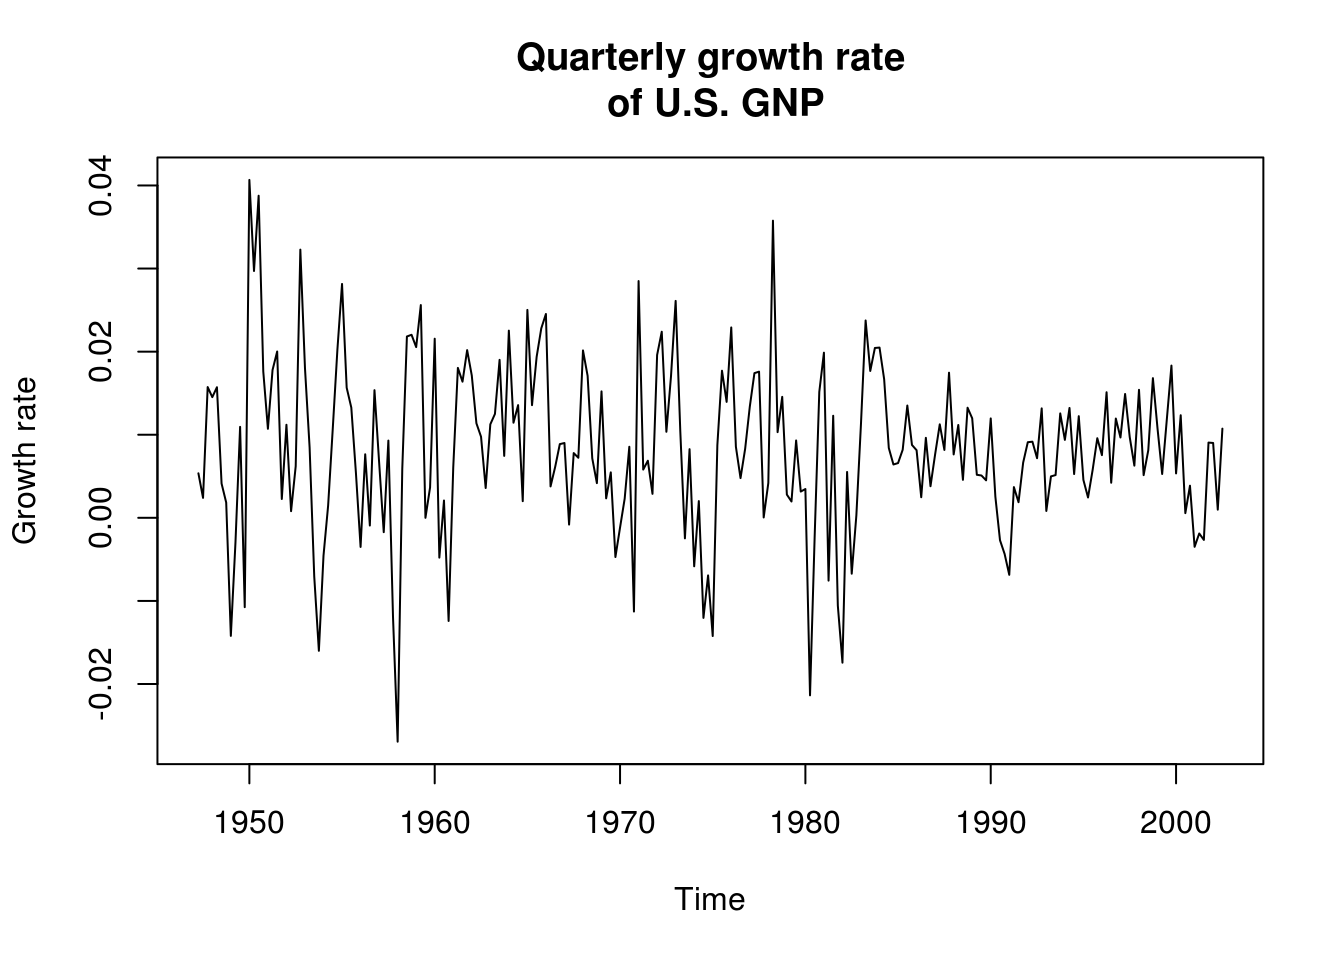
\includegraphics{timeseRies_files/figure-latex/unnamed-chunk-12-1.pdf}

\begin{Shaded}
\begin{Highlighting}[]
\CommentTok{# There is a different mean in each quarter, but forego the seasonal effect}
\CommentTok{# This is obvious in the following plot, which plots (in order), separating}
\CommentTok{# by quarter monthplot(gnpgr, main = main, ylab = 'Growth rate', xlab =}
\CommentTok{# 'Quarter')}
\KeywordTok{par}\NormalTok{(}\DataTypeTok{mfrow =} \KeywordTok{c}\NormalTok{(}\DecValTok{1}\NormalTok{, }\DecValTok{2}\NormalTok{))}
\NormalTok{TSA}\OperatorTok{::}\KeywordTok{acf}\NormalTok{(gnpgr, }\DecValTok{24}\NormalTok{, }\DataTypeTok{main =}\NormalTok{ main)}
\KeywordTok{pacf}\NormalTok{(gnpgr, }\DecValTok{24}\NormalTok{, }\DataTypeTok{main =}\NormalTok{ main)}
\end{Highlighting}
\end{Shaded}

\includegraphics{timeseRies_files/figure-latex/unnamed-chunk-12-2.pdf}

\begin{Shaded}
\begin{Highlighting}[]
\CommentTok{# What does the period in the correlogram correspond to?}
\end{Highlighting}
\end{Shaded}

The decrease in ACF/PACF suggests that either an AR(1) or an MA(2) might
be appropriate here.

\begin{Shaded}
\begin{Highlighting}[]
\NormalTok{mod1 <-}\StringTok{ }\KeywordTok{sarima}\NormalTok{(gnpgr, }\DataTypeTok{p =} \DecValTok{1}\NormalTok{, }\DataTypeTok{d =} \DecValTok{0}\NormalTok{, }\DataTypeTok{q =} \DecValTok{0}\NormalTok{, }\DataTypeTok{details =} \OtherTok{FALSE}\NormalTok{)  }\CommentTok{# AR(1)}
\KeywordTok{print}\NormalTok{(mod1}\OperatorTok{$}\NormalTok{ttable)}
\end{Highlighting}
\end{Shaded}

\begin{verbatim}
      Estimate     SE t.value p.value
ar1     0.3467 0.0627  5.5255       0
xmean   0.0083 0.0010  8.5398       0
\end{verbatim}

\begin{Shaded}
\begin{Highlighting}[]
\NormalTok{mod2 <-}\StringTok{ }\KeywordTok{sarima}\NormalTok{(gnpgr, }\DataTypeTok{p =} \DecValTok{0}\NormalTok{, }\DataTypeTok{d =} \DecValTok{0}\NormalTok{, }\DataTypeTok{q =} \DecValTok{2}\NormalTok{, }\DataTypeTok{details =} \OtherTok{FALSE}\NormalTok{)  }\CommentTok{# MA(2)}
\KeywordTok{print}\NormalTok{(mod2}\OperatorTok{$}\NormalTok{ttable)}
\end{Highlighting}
\end{Shaded}

\begin{verbatim}
      Estimate     SE t.value p.value
ma1     0.3028 0.0654  4.6272  0.0000
ma2     0.2035 0.0644  3.1594  0.0018
xmean   0.0083 0.0010  8.7178  0.0000
\end{verbatim}

Having fitted these two models, we compare them using their linear
proces (or MA(\(\infty\)) representation) and the theoretical
autocorrelation and partial autocorrelation coefficients.

\begin{Shaded}
\begin{Highlighting}[]
\CommentTok{# Obtain the coefficients from the MA(Inf)}
\KeywordTok{ARMAtoMA}\NormalTok{(}\DataTypeTok{ar =}\NormalTok{ mod1}\OperatorTok{$}\NormalTok{fit}\OperatorTok{$}\NormalTok{coef[}\DecValTok{1}\NormalTok{], }\DataTypeTok{ma =} \DecValTok{0}\NormalTok{, }\DecValTok{4}\NormalTok{)  }\CommentTok{# prints first 4 psi-weights}
\end{Highlighting}
\end{Shaded}

\begin{verbatim}
[1] 0.34665450 0.12016934 0.04165724 0.01444067
\end{verbatim}

\begin{Shaded}
\begin{Highlighting}[]
\CommentTok{# Print sample ACF and superpose the theoretical coefficients implied by the}
\CommentTok{# model}
\KeywordTok{par}\NormalTok{(}\DataTypeTok{mfrow =} \KeywordTok{c}\NormalTok{(}\DecValTok{1}\NormalTok{, }\DecValTok{2}\NormalTok{))}
\NormalTok{TSA}\OperatorTok{::}\KeywordTok{acf}\NormalTok{(gnpgr, }\DecValTok{10}\NormalTok{, }\DataTypeTok{main =}\NormalTok{ main)}
\KeywordTok{points}\NormalTok{(}\KeywordTok{seq}\NormalTok{(}\DecValTok{0}\NormalTok{, }\DataTypeTok{by =} \FloatTok{0.25}\NormalTok{, }\DataTypeTok{length =} \DecValTok{11}\NormalTok{), }\DataTypeTok{y =} \KeywordTok{ARMAacf}\NormalTok{(}\DataTypeTok{ar =}\NormalTok{ mod1}\OperatorTok{$}\NormalTok{fit}\OperatorTok{$}\NormalTok{coef[}\DecValTok{1}\NormalTok{], }\DataTypeTok{lag.max =} \DecValTok{10}\NormalTok{), }
    \DataTypeTok{col =} \StringTok{"blue"}\NormalTok{)}
\KeywordTok{points}\NormalTok{(}\KeywordTok{seq}\NormalTok{(}\DecValTok{0}\NormalTok{, }\DataTypeTok{by =} \FloatTok{0.25}\NormalTok{, }\DataTypeTok{length =} \DecValTok{11}\NormalTok{), }\DataTypeTok{y =} \KeywordTok{ARMAacf}\NormalTok{(}\DataTypeTok{ma =}\NormalTok{ mod2}\OperatorTok{$}\NormalTok{fit}\OperatorTok{$}\NormalTok{coef[}\DecValTok{1}\OperatorTok{:}\DecValTok{2}\NormalTok{], }
    \DataTypeTok{lag.max =} \DecValTok{10}\NormalTok{), }\DataTypeTok{col =} \StringTok{"red"}\NormalTok{)}

\KeywordTok{pacf}\NormalTok{(gnpgr, }\DecValTok{10}\NormalTok{, }\DataTypeTok{main =}\NormalTok{ main)}
\KeywordTok{points}\NormalTok{(}\KeywordTok{seq}\NormalTok{(}\FloatTok{0.25}\NormalTok{, }\DataTypeTok{by =} \FloatTok{0.25}\NormalTok{, }\DataTypeTok{length =} \DecValTok{10}\NormalTok{), }\DataTypeTok{y =} \KeywordTok{ARMAacf}\NormalTok{(}\DataTypeTok{ar =}\NormalTok{ mod1}\OperatorTok{$}\NormalTok{fit}\OperatorTok{$}\NormalTok{coef[}\DecValTok{1}\NormalTok{], }
    \DataTypeTok{lag.max =} \DecValTok{10}\NormalTok{, }\DataTypeTok{pacf =} \OtherTok{TRUE}\NormalTok{), }\DataTypeTok{col =} \StringTok{"blue"}\NormalTok{)}
\KeywordTok{points}\NormalTok{(}\KeywordTok{seq}\NormalTok{(}\FloatTok{0.25}\NormalTok{, }\DataTypeTok{by =} \FloatTok{0.25}\NormalTok{, }\DataTypeTok{length =} \DecValTok{10}\NormalTok{), }\DataTypeTok{y =} \KeywordTok{ARMAacf}\NormalTok{(}\DataTypeTok{ma =}\NormalTok{ mod2}\OperatorTok{$}\NormalTok{fit}\OperatorTok{$}\NormalTok{coef[}\DecValTok{1}\OperatorTok{:}\DecValTok{2}\NormalTok{], }
    \DataTypeTok{lag.max =} \DecValTok{10}\NormalTok{, }\DataTypeTok{pacf =} \OtherTok{TRUE}\NormalTok{), }\DataTypeTok{col =} \StringTok{"red"}\NormalTok{)}
\end{Highlighting}
\end{Shaded}

\includegraphics{timeseRies_files/figure-latex/gnp_ar1orma2_comparison-1.pdf}

\textbf{Warning}: in the example above, it is necessary here to add a
constant coefficient. Economic theory suggest exponential growth, hence
a trend of \(\exp(t \beta)\). This becomes a linear trend \(t\beta\) for
log returns, and by differencing, we obtain the trend \(\beta\). The
latter corresponds to the long term trend, or the quarterly growth rate,
which is about 1\%. The coefficient is significant even if it seems
small and failing to include it leads to invalid inference about the
state of the U.S. economy.

The last step is to check whether our process is causal and invertible.
For the former, \texttt{arima} typically transforms to the stationary
and invertible solution, so we should be good. We may end up having a
root of \(\Phi(B)\) or \(\Theta(B)\) on the unit circle. In this case,
the ARMA process is not stationary, while in the second, asymptotic
normality of the estimator breaks down. We look at the roots of the
polynomial \(\Phi(B)\) and \(\Theta(B)\) and check they indeed are
outside the unit circle. It is easiest to check their norm or modulus.

\begin{Shaded}
\begin{Highlighting}[]
\CommentTok{# Is the MA(2) process invertible?}
\KeywordTok{abs}\NormalTok{(}\KeywordTok{polyroot}\NormalTok{(}\KeywordTok{c}\NormalTok{(}\DecValTok{1}\NormalTok{, mod2}\OperatorTok{$}\NormalTok{fit}\OperatorTok{$}\NormalTok{coef[}\DecValTok{1}\OperatorTok{:}\DecValTok{2}\NormalTok{])))  }\CommentTok{#MA roots}
\end{Highlighting}
\end{Shaded}

\begin{verbatim}
[1] 2.216653 2.216653
\end{verbatim}

\begin{Shaded}
\begin{Highlighting}[]
\CommentTok{# Is the AR(1) process causal}
\KeywordTok{Mod}\NormalTok{(}\KeywordTok{polyroot}\NormalTok{(}\KeywordTok{c}\NormalTok{(}\DecValTok{1}\NormalTok{, }\OperatorTok{-}\NormalTok{mod1}\OperatorTok{$}\NormalTok{fit}\OperatorTok{$}\NormalTok{coef[}\DecValTok{1}\NormalTok{])))  }\CommentTok{#AR roots}
\end{Highlighting}
\end{Shaded}

\begin{verbatim}
[1] 2.884717
\end{verbatim}

Sometimes models give similar output. The model choice should then be
made on the grounds of \textbf{parsimony}: a simpler model that explains
the data should be prefered. If the models are nested, for example an
AR(1) and an AR(2), then a likelihood ratio test can be performed (watch
out to make sure the same number of observations appear in the models if
using a conditional likelihood). A quick way to do this is by looking at
the Akaike's information criterion. There are other information
criterion, notably the BIC and bias-corrected version of AIC termed
\(\mathrm{AIC}_{\mathrm{c}}\). They are defined respectively as

\[
\begin{align*}
\mathrm{AIC}& = -2\ell(\boldsymbol{\theta})+2k,\\
\mathrm{BIC}& = -2\ell(\boldsymbol{\theta})+k\log(n),\\
\mathrm{AIC}_{\mathrm{c}}& = -2\ell(\boldsymbol{\theta})+2 \frac{kn}{n-k-1}.
\end{align*}
\]

In the formulas above, \(n\) is the sample size, \(k\) is the number of
parameters in the model and \(\ell\) is log-likelihood. Since likelihood
values increase with the number of parameters provided the models are
nested (why?), the additional term penalizes complex models. The
Schwartz's information criterion (or Bayesian information criterion, BIC
in short) includes the sample size in the penalty. The penalty could be
viewed as a testing procedure similar to likelihood ratio test for
nested models, where in place of the quantiles of the \(\chi^2\)
distribution, one uses e.g.~for AIC a threshold of \(2(k_1-k_2)\).

The BIC is consistent, meaning that it chooses the correct model with
probability 1 as \(n \to \infty\). AIC is \emph{not} consistent for
model selection and this results typically in overfitting. For ARMA
models models with zero mean, Brockwell and Davis advocate the use of a
small-sample correction of AIC, AIC\(_\mathrm{c}\), with \(k = p+q+1\).
The latter is equivalent to AIC when \(n \to \infty\).

\textbf{Warning}: The information criterion returned by
\texttt{astsa::sarima} does not correspond to the definition above; the
one implemented can be found in Shumway and Stoffer's book. The
principle remains the same: the lower, the better.

Here is an illustrative example on the dataset in the following exercise
with a helper function to find the roots of the polynomials. I would
like to bring your attention to the fact about the difficulties of
optimizing some time series models. For example, one often finds that
the ARMA(2,1) fits as well as the AR(1), even when the latter is the
true underlying model. However, a quick look at the output below is
illustrative of the trouble that lies ahead.

In the next exercise, you will be asked to practice your skills on
simulated datasets. Before letting you proceed, I want to illustrate the
different commands for fitting e.g.~an ARMA(2, 1) model, and see what
comes out.

\begin{Shaded}
\begin{Highlighting}[]
\KeywordTok{library}\NormalTok{(forecast)}
\KeywordTok{library}\NormalTok{(astsa)}
\KeywordTok{load}\NormalTok{(}\KeywordTok{url}\NormalTok{(}\StringTok{"http://sma.epfl.ch/~lbelzile/math342/Simulated_ARMA.RData"}\NormalTok{))}

\CommentTok{# Wrapper around arima from forecast library}
\NormalTok{mod_a <-}\StringTok{ }\KeywordTok{arima}\NormalTok{(x3, }\DataTypeTok{order =} \KeywordTok{c}\NormalTok{(}\DecValTok{2}\NormalTok{, }\DecValTok{0}\NormalTok{, }\DecValTok{1}\NormalTok{), }\DataTypeTok{transform.pars =} \OtherTok{TRUE}\NormalTok{)}
\NormalTok{mod_b <-}\StringTok{ }\KeywordTok{Arima}\NormalTok{(x3, }\DataTypeTok{order =} \KeywordTok{c}\NormalTok{(}\DecValTok{2}\NormalTok{, }\DecValTok{0}\NormalTok{, }\DecValTok{1}\NormalTok{), }\DataTypeTok{transform.pars =} \OtherTok{TRUE}\NormalTok{)}
\CommentTok{# Arima returns BIC, AIC and AICC}
\NormalTok{mod_c <-}\StringTok{ }\KeywordTok{sarima}\NormalTok{(x3, }\DataTypeTok{p =} \DecValTok{2}\NormalTok{, }\DataTypeTok{d =} \DecValTok{0}\NormalTok{, }\DataTypeTok{q =} \DecValTok{1}\NormalTok{, }\DataTypeTok{details =} \OtherTok{FALSE}\NormalTok{)}
\end{Highlighting}
\end{Shaded}

\includegraphics{timeseRies_files/figure-latex/unnamed-chunk-13-1.pdf}

\begin{Shaded}
\begin{Highlighting}[]
\CommentTok{# sarima provides diagnostic plots unless `details=FALSE` unfortunately also}
\CommentTok{# returns all the optimization steps from `arima` in the new version}
\NormalTok{mod_a}
\end{Highlighting}
\end{Shaded}

\begin{verbatim}

Call:
arima(x = x3, order = c(2, 0, 1), transform.pars = TRUE)

Coefficients:
         ar1      ar2     ma1  intercept
      1.0872  -0.3739  0.9621    -0.6908
s.e.  0.1142   0.1182  0.1310     0.5769

sigma^2 estimated as 0.7271:  log likelihood = -128.77,  aic = 267.54
\end{verbatim}

\begin{Shaded}
\begin{Highlighting}[]
\NormalTok{mod_b}
\end{Highlighting}
\end{Shaded}

\begin{verbatim}
Series: x3 
ARIMA(2,0,1) with non-zero mean 

Coefficients:
         ar1      ar2     ma1     mean
      1.0872  -0.3739  0.9621  -0.6908
s.e.  0.1142   0.1182  0.1310   0.5769

sigma^2 estimated as 0.7574:  log likelihood=-128.77
AIC=267.54   AICc=268.18   BIC=280.57
\end{verbatim}

\begin{Shaded}
\begin{Highlighting}[]
\NormalTok{mod_c}
\end{Highlighting}
\end{Shaded}

\begin{verbatim}
$fit

Call:
stats::arima(x = xdata, order = c(p, d, q), seasonal = list(order = c(P, D, 
    Q), period = S), xreg = xmean, include.mean = FALSE, optim.control = list(trace = trc, 
    REPORT = 1, reltol = tol))

Coefficients:
         ar1      ar2     ma1    xmean
      1.0872  -0.3739  0.9621  -0.6908
s.e.  0.1142   0.1182  0.1310   0.5769

sigma^2 estimated as 0.7271:  log likelihood = -128.77,  aic = 267.54

$degrees_of_freedom
[1] 96

$ttable
      Estimate     SE t.value p.value
ar1     1.0872 0.1142  9.5220  0.0000
ar2    -0.3739 0.1182 -3.1627  0.0021
ma1     0.9621 0.1310  7.3417  0.0000
xmean  -0.6908 0.5769 -1.1973  0.2341

$AIC
[1] 0.7612783

$AICc
[1] 0.7876612

$BIC
[1] -0.1345149
\end{verbatim}

You can (and should) check the roots of the AR and MA polynomials to
make sure this is not happening. The argument \texttt{transform.pars}
transforms the AR polynomial to the causal representation if it does not
have a root on the unit circle. If the process is not invertible, the
parameter lies on the boundary of the space and the usual standard
errors obtained from the observed information matrix are not reliable.
It is possible to use these models for forecasting, but their
interpretation is awkward.

\subsection{Exercise 2: Simulated
series}\label{exercise-2-simulated-series}

\begin{enumerate}
\def\labelenumi{\arabic{enumi}.}
\tightlist
\item
  The \texttt{Simulated\_ARMA} dataset contains 8 time series (these
  examples are from Charlotte Wickham's website). Fit ARMA models to
  those and select a model, justifying your choice. Be skeptical of the
  optimization routine and analyze the models carefully.
\end{enumerate}

\section{Information criterion, model selection and profile
likelihood}\label{information-criterion-model-selection-and-profile-likelihood}

The following example is due to
\href{http://ionides.github.io/531w16/notes05/notes5.html}{Edward
Ionides} and is licensed under CC-BY-NC.

We analyze data from NOAA, the depth of Lake Huron (in m). There is a
decreasing trend. We first format the time variable and extract the
height in January.

\begin{Shaded}
\begin{Highlighting}[]
\KeywordTok{library}\NormalTok{(lubridate)}
\CommentTok{# Data from}
\CommentTok{# http://www.glerl.noaa.gov/data/dashboard/data/levels/mGauge/miHuronMog.csv}
\NormalTok{dat <-}\StringTok{ }\KeywordTok{read.csv}\NormalTok{(}\StringTok{"http://sma.epfl.ch/~lbelzile/math342/huron_depth.csv"}\NormalTok{, }\DataTypeTok{sep =} \StringTok{","}\NormalTok{, }
    \DataTypeTok{header =} \OtherTok{TRUE}\NormalTok{, }\DataTypeTok{skip =} \DecValTok{2}\NormalTok{)}
\NormalTok{dat}\OperatorTok{$}\NormalTok{Date <-}\StringTok{ }\KeywordTok{strptime}\NormalTok{(dat}\OperatorTok{$}\NormalTok{Date, }\StringTok{"%m/%d/%Y"}\NormalTok{)}
\NormalTok{dat}\OperatorTok{$}\NormalTok{year <-}\StringTok{ }\KeywordTok{with}\NormalTok{(dat, }\KeywordTok{year}\NormalTok{(Date))}
\NormalTok{dat}\OperatorTok{$}\NormalTok{month <-}\StringTok{ }\KeywordTok{with}\NormalTok{(dat, }\KeywordTok{month}\NormalTok{(Date))  }\CommentTok{#as.numeric(format(dat$Date, format = '%m'))}
\KeywordTok{head}\NormalTok{(dat)}
\end{Highlighting}
\end{Shaded}

\begin{verbatim}
        Date Average year month
1 1860-01-01 177.285 1860     1
2 1860-02-01 177.339 1860     2
3 1860-03-01 177.349 1860     3
4 1860-04-01 177.388 1860     4
5 1860-05-01 177.425 1860     5
6 1860-06-01 177.461 1860     6
\end{verbatim}

\begin{Shaded}
\begin{Highlighting}[]
\NormalTok{## Subsample values to take only January data}
\NormalTok{dat <-}\StringTok{ }\KeywordTok{subset}\NormalTok{(dat, month }\OperatorTok{==}\StringTok{ }\DecValTok{1}\NormalTok{)}
\NormalTok{huron_depth <-}\StringTok{ }\NormalTok{dat}\OperatorTok{$}\NormalTok{Average}
\NormalTok{year <-}\StringTok{ }\NormalTok{dat}\OperatorTok{$}\NormalTok{year}
\CommentTok{# Plot the series}
\KeywordTok{plot}\NormalTok{(huron_depth }\OperatorTok{~}\StringTok{ }\NormalTok{year, }\DataTypeTok{type =} \StringTok{"l"}\NormalTok{, }\DataTypeTok{ylab =} \StringTok{"Lake depth (m)"}\NormalTok{, }\DataTypeTok{main =} \StringTok{"Monthly Average Master Gauge}\CharTok{\textbackslash{}n}\StringTok{Water Levels (1860-Present)"}\NormalTok{)}
\end{Highlighting}
\end{Shaded}

\includegraphics{timeseRies_files/figure-latex/lake_huronf-1.pdf}

Next, we create a table containing the AIC values, which are obtained
from fitting successive ARMA models with varying orders \(p\), \(q\).
Here, a simple AR(1) does an excellent job at capturing the structure
and all other models are essentially more complicated versions.

\begin{Shaded}
\begin{Highlighting}[]
\NormalTok{huron_ar1 <-}\StringTok{ }\KeywordTok{Arima}\NormalTok{(huron_depth, }\DataTypeTok{order =} \KeywordTok{c}\NormalTok{(}\DecValTok{1}\NormalTok{, }\DecValTok{0}\NormalTok{, }\DecValTok{0}\NormalTok{), }\DataTypeTok{include.drift =} \OtherTok{TRUE}\NormalTok{, }\DataTypeTok{include.mean =} \OtherTok{TRUE}\NormalTok{)}

\NormalTok{## Table of AIC values extracted from the output - notice the warnings on}
\NormalTok{## your computer when the fit fails!}
\NormalTok{aic_table <-}\StringTok{ }\ControlFlowTok{function}\NormalTok{(data, P, Q) \{}
\NormalTok{    table <-}\StringTok{ }\KeywordTok{matrix}\NormalTok{(}\OtherTok{NA}\NormalTok{, (P }\OperatorTok{+}\StringTok{ }\DecValTok{1}\NormalTok{), (Q }\OperatorTok{+}\StringTok{ }\DecValTok{1}\NormalTok{))}
    \ControlFlowTok{for}\NormalTok{ (p }\ControlFlowTok{in} \DecValTok{0}\OperatorTok{:}\NormalTok{P) \{}
        \ControlFlowTok{for}\NormalTok{ (q }\ControlFlowTok{in} \DecValTok{0}\OperatorTok{:}\NormalTok{Q) \{}
\NormalTok{            table[p }\OperatorTok{+}\StringTok{ }\DecValTok{1}\NormalTok{, q }\OperatorTok{+}\StringTok{ }\DecValTok{1}\NormalTok{] <-}\StringTok{ }\KeywordTok{arima}\NormalTok{(data, }\DataTypeTok{order =} \KeywordTok{c}\NormalTok{(p, }\DecValTok{0}\NormalTok{, q))}\OperatorTok{$}\NormalTok{aic}
\NormalTok{        \}}
\NormalTok{    \}}
    \KeywordTok{dimnames}\NormalTok{(table) <-}\StringTok{ }\KeywordTok{list}\NormalTok{(}\KeywordTok{paste}\NormalTok{(}\StringTok{"<b> AR"}\NormalTok{, }\DecValTok{0}\OperatorTok{:}\NormalTok{P, }\StringTok{"</b>"}\NormalTok{, }\DataTypeTok{sep =} \StringTok{""}\NormalTok{), }\KeywordTok{paste}\NormalTok{(}\StringTok{"MA"}\NormalTok{, }
        \DecValTok{0}\OperatorTok{:}\NormalTok{Q, }\DataTypeTok{sep =} \StringTok{""}\NormalTok{))}
\NormalTok{    table}
\NormalTok{\}}
\NormalTok{huron_aic_table <-}\StringTok{ }\KeywordTok{aic_table}\NormalTok{(huron_depth, }\DecValTok{4}\NormalTok{, }\DecValTok{5}\NormalTok{)}
\KeywordTok{require}\NormalTok{(knitr)}
\KeywordTok{kable}\NormalTok{(huron_aic_table, }\DataTypeTok{digits =} \DecValTok{2}\NormalTok{)}
\end{Highlighting}
\end{Shaded}

\begin{tabular}{l|r|r|r|r|r|r}
\hline
  & MA0 & MA1 & MA2 & MA3 & MA4 & MA5\\
\hline
<b> AR0</b> & 166.75 & 46.60 & 7.28 & -14.97 & -18.64 & -26.09\\
\hline
<b> AR1</b> & -38.00 & -37.41 & -35.46 & -33.82 & -34.13 & -32.20\\
\hline
<b> AR2</b> & -37.33 & -38.43 & -36.90 & -34.93 & -34.35 & -33.08\\
\hline
<b> AR3</b> & -35.52 & -35.17 & -32.71 & -31.38 & -31.13 & -32.98\\
\hline
<b> AR4</b> & -33.94 & -34.91 & -34.43 & -36.27 & -31.31 & -30.90\\
\hline
\end{tabular}

\begin{Shaded}
\begin{Highlighting}[]
\NormalTok{## Kables are tables for HTML. For LaTeX, use something like library(xtable)}
\NormalTok{## dimnames(huron_aic_table) <- list(paste0('AR', 0:4), paste0('MA', 0:5))}
\NormalTok{## latex_tab <- xtable::xtable(huron_aic_table, booktabs = TRUE, caption =}
\NormalTok{## 'AIC values for ARMA models for the Lake Huron dataset') print(latex_tab,}
\NormalTok{## booktabs = TRUE, caption.placement = 'top')}
\end{Highlighting}
\end{Shaded}

I silenced the output, but some of the optimization routine
\emph{failed} (duh). You can see this by looking at the AIC values
(recall the definition and look at nested models). These cannot increase
by more than 2 from left to right or top to bottom.

Subsequent quotes are from Prof.~Ionides' notes

\begin{quote}
What do we learn by interpreting the results in the above table of AIC
values? In what ways might we have to be careful not to over-interpret
the results of this table?
\end{quote}

We can look at the roots to see if the process of our choice (the one
with lowest AIC, say) is good. Overly complicated models can lead you to
big troubles. We illustrate this by fitting a complex model, an
ARMA(2,1), to the series:

\begin{Shaded}
\begin{Highlighting}[]
\NormalTok{## Fit an ARMA(2, 1) model}
\NormalTok{huron_arma21 <-}\StringTok{ }\KeywordTok{Arima}\NormalTok{(huron_depth, }\DataTypeTok{order =} \KeywordTok{c}\NormalTok{(}\DecValTok{2}\NormalTok{, }\DecValTok{0}\NormalTok{, }\DecValTok{1}\NormalTok{), }\DataTypeTok{include.drift =} \OtherTok{TRUE}\NormalTok{, }
    \DataTypeTok{include.mean =} \OtherTok{TRUE}\NormalTok{)}
\NormalTok{huron_arma21}
\end{Highlighting}
\end{Shaded}

\begin{verbatim}
Series: huron_depth 
ARIMA(2,0,1) with drift 

Coefficients:
          ar1     ar2     ma1  intercept    drift
      -0.0979  0.7464  1.0000   176.8391  -0.0049
s.e.   0.0553  0.0554  0.0244     0.1734   0.0019

sigma^2 estimated as 0.04188:  log likelihood=26.89
AIC=-41.78   AICc=-41.22   BIC=-23.52
\end{verbatim}

\begin{Shaded}
\begin{Highlighting}[]
\NormalTok{## Root of the Phi polynomial}
\NormalTok{AR_roots <-}\StringTok{ }\KeywordTok{polyroot}\NormalTok{(}\KeywordTok{c}\NormalTok{(}\DecValTok{1}\NormalTok{, }\OperatorTok{-}\KeywordTok{coef}\NormalTok{(huron_arma21)[}\KeywordTok{grep}\NormalTok{(}\StringTok{"^ar"}\NormalTok{, }\KeywordTok{names}\NormalTok{(huron_arma21}\OperatorTok{$}\NormalTok{coef))]))}
\KeywordTok{Mod}\NormalTok{(AR_roots)}
\end{Highlighting}
\end{Shaded}

\begin{verbatim}
[1] 1.224905 1.093792
\end{verbatim}

The process is causal, but the estimate of the MA coefficient,
\(\theta_1\) is on the boundary of the parameter space and numerically
indistinguishable from 1.

\begin{quote}
Let's investigate a little, using profile methods. The claimed standard
error on the MA(1) coefficient, from the Fisher information approach
used by \texttt{arima} is small. We can see if the approximate
confidence interval constructed using profile likelihood is in agreement
with the approximate confidence interval constructed using the observed
Fisher information.
\end{quote}

\begin{quote}
Note that \texttt{arima} transforms the model to invertibility. Thus,
the estimated value of \(\theta_1\) can only fall in the interval
\((−1, 1)\) but can be arbitrarily close to \(−1\) or \(1\).
\end{quote}

Recall the definition of profile likelihood: for a parameter of interest
\(\boldsymbol{\psi}\) and a partition
\(\boldsymbol{\theta}=(\boldsymbol{\psi}, \boldsymbol{\lambda})\), the
profile likelihood as a function of \(\boldsymbol{\psi}\) is
\[\ell_p(\boldsymbol{\psi}) = \mathrm{argmax}_{\boldsymbol{\lambda} \in \Lambda} \ell(\boldsymbol{\lambda} \mid \boldsymbol{\psi}).\]

The maximum profile likelihood coincides with the maximum likelihood
estimate (why?), and we use it normally to obtain more accurate
confidence intervals for (a) parameter(s) of interest. Here, we
investigate the profile log-likelihood of the MA(1) coefficient. Unlike
the nice examples you saw in class, the profile here is weird and the
global maximum lies on the boundary.

\begin{Shaded}
\begin{Highlighting}[]
\NormalTok{## Profile log-likelihood for the MA coefficient}
\NormalTok{K <-}\StringTok{ }\DecValTok{1000}
\NormalTok{ma1 <-}\StringTok{ }\KeywordTok{seq}\NormalTok{(}\DataTypeTok{from =} \OperatorTok{-}\FloatTok{0.99}\NormalTok{, }\DataTypeTok{to =} \DecValTok{1}\NormalTok{, }\DataTypeTok{length =}\NormalTok{ K)}
\NormalTok{profile_loglik <-}\StringTok{ }\KeywordTok{rep}\NormalTok{(}\OtherTok{NA}\NormalTok{, K)}
\ControlFlowTok{for}\NormalTok{ (k }\ControlFlowTok{in} \DecValTok{1}\OperatorTok{:}\NormalTok{K) \{}
\NormalTok{    profile_loglik[k] <-}\StringTok{ }\KeywordTok{logLik}\NormalTok{(}\KeywordTok{arima}\NormalTok{(huron_depth, }\DataTypeTok{order =} \KeywordTok{c}\NormalTok{(}\DecValTok{2}\NormalTok{, }\DecValTok{0}\NormalTok{, }\DecValTok{1}\NormalTok{), }\DataTypeTok{xreg =} \KeywordTok{scale}\NormalTok{(}\KeywordTok{seq}\NormalTok{(}\DecValTok{1}\OperatorTok{:}\KeywordTok{length}\NormalTok{(huron_depth))), }
        \DataTypeTok{include.mean =} \OtherTok{TRUE}\NormalTok{, }\DataTypeTok{fixed =} \KeywordTok{c}\NormalTok{(}\OtherTok{NA}\NormalTok{, }\OtherTok{NA}\NormalTok{, ma1[k], }\OtherTok{NA}\NormalTok{, }\OtherTok{NA}\NormalTok{)))}
\NormalTok{\}}
\CommentTok{# Failed for some values of the MA}
\KeywordTok{plot}\NormalTok{(profile_loglik }\OperatorTok{-}\StringTok{ }\KeywordTok{logLik}\NormalTok{(huron_arma21) }\OperatorTok{~}\StringTok{ }\NormalTok{ma1, }\DataTypeTok{type =} \StringTok{"l"}\NormalTok{, }\DataTypeTok{ylab =} \StringTok{"Profile log likelihood"}\NormalTok{, }
    \DataTypeTok{xlab =} \StringTok{"value"}\NormalTok{, }\DataTypeTok{main =} \KeywordTok{expression}\NormalTok{(}\KeywordTok{paste}\NormalTok{(}\StringTok{"Profile log-likelihood of "}\NormalTok{, theta[}\DecValTok{1}\NormalTok{], }
        \StringTok{" for the ARMA(2, 1) model"}\NormalTok{)))}
\KeywordTok{abline}\NormalTok{(}\DataTypeTok{h =} \OperatorTok{-}\KeywordTok{qchisq}\NormalTok{(}\FloatTok{0.95}\NormalTok{, }\DecValTok{1}\NormalTok{)}\OperatorTok{/}\DecValTok{2}\NormalTok{, }\DataTypeTok{col =} \DecValTok{2}\NormalTok{, }\DataTypeTok{lty =} \DecValTok{2}\NormalTok{)}
\KeywordTok{abline}\NormalTok{(}\DataTypeTok{v =} \DecValTok{1}\NormalTok{, }\DataTypeTok{col =} \DecValTok{1}\NormalTok{)}
\end{Highlighting}
\end{Shaded}

\includegraphics{timeseRies_files/figure-latex/profile_confint-1.pdf}

The ``usual'' 95\% profile confidence interval would thus include zero,
so the coefficient is maybe not significant after all. I coded a little
function that you can use to find the value at which a profile
log-likelihood, here shifted so that the maximum is at zero, intersects
with the value of half the \(\chi^2\) quantile.

\begin{Shaded}
\begin{Highlighting}[]
\CommentTok{# mle <- logLik(huron_arma21)[1]}
\NormalTok{profile_confint <-}\StringTok{ }\ControlFlowTok{function}\NormalTok{(mle, xvals, profile, }\DataTypeTok{lev =} \FloatTok{0.95}\NormalTok{) \{}
\NormalTok{    K <-}\StringTok{ }\KeywordTok{length}\NormalTok{(profile)}
\NormalTok{    ind_max <-}\StringTok{ }\KeywordTok{which.max}\NormalTok{(profile)  }\CommentTok{#value corresponding to MLE}
\NormalTok{    val_conf <-}\StringTok{ }\NormalTok{mle }\OperatorTok{-}\StringTok{ }\KeywordTok{qchisq}\NormalTok{(lev, }\DecValTok{1}\NormalTok{)}\OperatorTok{/}\DecValTok{2}  \CommentTok{#Cutoff line}
    
    \CommentTok{# Find the closest value by linear interpolation, swapping x and y}
\NormalTok{    upper <-}\StringTok{ }\NormalTok{profile[(ind_max }\OperatorTok{+}\StringTok{ }\DecValTok{1}\NormalTok{)}\OperatorTok{:}\NormalTok{K]}
\NormalTok{    lower <-}\StringTok{ }\NormalTok{profile[}\DecValTok{1}\OperatorTok{:}\NormalTok{ind_max]}
\NormalTok{    up <-}\StringTok{ }\KeywordTok{suppressWarnings}\NormalTok{(}\KeywordTok{c}\NormalTok{(}\KeywordTok{max}\NormalTok{(}\KeywordTok{which}\NormalTok{(upper }\OperatorTok{>=}\StringTok{ }\NormalTok{val_conf)), }\KeywordTok{min}\NormalTok{(}\KeywordTok{which}\NormalTok{(upper }\OperatorTok{<}\StringTok{ }
\StringTok{        }\NormalTok{val_conf))) }\OperatorTok{+}\StringTok{ }\NormalTok{ind_max)}
\NormalTok{    low <-}\StringTok{ }\KeywordTok{suppressWarnings}\NormalTok{(}\KeywordTok{c}\NormalTok{(}\KeywordTok{min}\NormalTok{(}\KeywordTok{which}\NormalTok{(lower }\OperatorTok{>=}\StringTok{ }\NormalTok{val_conf)), }\KeywordTok{max}\NormalTok{(}\KeywordTok{which}\NormalTok{(lower }\OperatorTok{<}\StringTok{ }
\StringTok{        }\NormalTok{val_conf))))}
    \CommentTok{# Linear interpolation step with two closest values}
    \ControlFlowTok{if}\NormalTok{ (}\OperatorTok{!}\KeywordTok{any}\NormalTok{(}\KeywordTok{is.infinite}\NormalTok{(low))) \{}
\NormalTok{        a <-}\StringTok{ }\KeywordTok{approx}\NormalTok{(}\DataTypeTok{y =}\NormalTok{ ma1[low], }\DataTypeTok{x =}\NormalTok{ profile_loglik[low], }\DataTypeTok{xout =}\NormalTok{ val_conf[}\DecValTok{1}\NormalTok{])}\OperatorTok{$}\NormalTok{y}
\NormalTok{    \} }\ControlFlowTok{else}\NormalTok{ \{}
        \KeywordTok{warning}\NormalTok{(}\StringTok{"No value of the profile likelihood is below the threshold}
\StringTok{           for the lower confidence interval"}\NormalTok{)}
\NormalTok{        a <-}\StringTok{ }\OtherTok{NA}
\NormalTok{    \}}
    \ControlFlowTok{if}\NormalTok{ (}\OperatorTok{!}\KeywordTok{any}\NormalTok{(}\KeywordTok{is.infinite}\NormalTok{(up))) \{}
\NormalTok{        b <-}\StringTok{ }\KeywordTok{approx}\NormalTok{(}\DataTypeTok{y =}\NormalTok{ ma1[up], }\DataTypeTok{x =}\NormalTok{ profile_loglik[up], }\DataTypeTok{xout =}\NormalTok{ val_conf[}\DecValTok{1}\NormalTok{])}\OperatorTok{$}\NormalTok{y}
\NormalTok{    \} }\ControlFlowTok{else}\NormalTok{ \{}
        \KeywordTok{warning}\NormalTok{(}\StringTok{"No value of the profile likelihood is below the threshold}
\StringTok{           for the upper confidence interval"}\NormalTok{)}
\NormalTok{        b <-}\StringTok{ }\OtherTok{NA}
\NormalTok{    \}}
    \KeywordTok{return}\NormalTok{(}\KeywordTok{c}\NormalTok{(a, b))}
\NormalTok{\}}
\CommentTok{# Profile confidence interval}
\KeywordTok{profile_confint}\NormalTok{(}\KeywordTok{logLik}\NormalTok{(huron_arma21)[}\DecValTok{1}\NormalTok{], }\DataTypeTok{xvals =}\NormalTok{ ma1, }\DataTypeTok{profile =}\NormalTok{ profile_loglik, }
    \DataTypeTok{lev =} \FloatTok{0.95}\NormalTok{)}
\end{Highlighting}
\end{Shaded}

\begin{verbatim}
[1] -0.5260204         NA
\end{verbatim}

Here, the ``usual'' 95\% confidence interval includes (because of the
constraint) all values in (-0.53, 1).

\begin{quote}
\begin{itemize}
\tightlist
\item
  What do you conclude about the Fisher information confidence interval
  proposed by \texttt{arima}?
\item
  When do you think the Fisher information confidence interval may be
  reliable?
\item
  Is this profile likelihood plot, and its statistical interpretation,
  reliable? How do you support your opinion on this?
\end{itemize}
\end{quote}

Be suspicious of the output and think before acting.

There is in fact a non-zero probability of obtaining a coefficient of
\(\pm 1\) for an MA(1). This can be easily seen through a simulation. We
see a picture that roughly matches that of the profile likelihood
(noting what seems to be convergence to a local maximum at \(\theta=-1\)
in many cases).

\begin{Shaded}
\begin{Highlighting}[]
\KeywordTok{set.seed}\NormalTok{(}\DecValTok{54321}\NormalTok{)}
\KeywordTok{hist}\NormalTok{(MAcoefdist <-}\StringTok{ }\KeywordTok{replicate}\NormalTok{(}\DataTypeTok{n=}\DecValTok{1000}\NormalTok{, }\CommentTok{#perform 1000 replicates}
      \KeywordTok{coef}\NormalTok{(}\KeywordTok{Arima}\NormalTok{(}\DataTypeTok{order=}\KeywordTok{c}\NormalTok{(}\DecValTok{2}\NormalTok{,}\DecValTok{0}\NormalTok{,}\DecValTok{1}\NormalTok{),  }\CommentTok{#extract ma[1] coef from ARMA(2,1)}
\KeywordTok{arima.sim}\NormalTok{(}\DataTypeTok{n=}\DecValTok{155}\NormalTok{, }\DataTypeTok{model=}\KeywordTok{list}\NormalTok{(}\DataTypeTok{ar=}\KeywordTok{coef}\NormalTok{(huron_ar1)[}\StringTok{"ar1"}\NormalTok{])),))[}\StringTok{"ma1"}\NormalTok{]), }\CommentTok{#data is 155 obs from AR(1) model}
\DataTypeTok{breaks=}\DecValTok{300}\NormalTok{, }\DataTypeTok{main=}\StringTok{"Estimate of the MA(1) coefficient}\CharTok{\textbackslash{}n}\StringTok{ in an ARMA(1,2) model"}\NormalTok{, }\DataTypeTok{xlab=}\StringTok{"MA(1) coefficient value"}\NormalTok{)}
\end{Highlighting}
\end{Shaded}

\includegraphics{timeseRies_files/figure-latex/madist_sim-1.pdf}

\begin{Shaded}
\begin{Highlighting}[]
\CommentTok{#Proportion of values that lie on the boundary.}
\KeywordTok{mean}\NormalTok{(}\KeywordTok{I}\NormalTok{(}\KeywordTok{abs}\NormalTok{(MAcoefdist)}\OperatorTok{>}\FloatTok{0.999}\NormalTok{))}
\end{Highlighting}
\end{Shaded}

\begin{verbatim}
[1] 0.069
\end{verbatim}

We wish to restrict to causal and invertible processes. The latter
implies that the AR(\(\infty\)) representation of the process exists;
the latter is used for prediction. However, while unit roots happen
rarely, you only get one sample and it may happen in yours. This makes
life more complicated because the asymptotics are non-regular for the
problem. It is thus best to rely on procedures that only require
estimation of the model under the null hypothesis, such as a score test.

\subsection{Exercise 3: Lake Erie
height}\label{exercise-3-lake-erie-height}

\begin{enumerate}
\def\labelenumi{\arabic{enumi}.}
\tightlist
\item
  Perform an additive decomposition of the form
  \[Y_t = m_t + s_t + Z_t\] where \(m_t\) is the trend and \(s_t\) is a
  seasonal component of the Lake Erie height series, found at
  \href{\%5Bhttp://sma.epfl.ch/~lbelzile/math342/LakeErie.csv\%5D}{http://sma.epfl.ch/\textasciitilde{}lbelzile/math342/LakeErie.csv}.
  Characterize the stochastic component \(Z_t\) using an ARMA model.
\item
  Obtain a table of AIC and BIC values for ARMA(\(p, q\)) model for
  order 7 and less. Anything worth of notice?
\item
  Justifying your answer, select an adequate ARMA model. Are the
  residuals from this model white noise?
\item
  Look at the fitted model and check for invertibility and causality of
  your solution.
\item
  Plot the (partial) correlogram of \(Z_t\) and superpose the
  theoretical coefficients implied by your model.
\item
  Plot the correlogram of the residuals of your ARMA model. Do they
  appear white noise?
\item
  Perform a Ljung-Box test on the residuals. What can you conclude?
\end{enumerate}

\section{Solutions to Exercises}\label{solutions-to-exercises-1}

\subsection{Exercise 1: UBS stock
returns}\label{exercise-1-ubs-stock-returns-1}

\begin{enumerate}
\def\labelenumi{\arabic{enumi}.}
\tightlist
\item
  Create a function that fits an AR(1)-ARCH(1) model by modifying the
  code provided above and apply it to \texttt{y}.
\item
  Obtain the maximum likelihood estimates using \texttt{nlm} or
  \texttt{optim} as well as the standard errors
\item
  Make a residual plot. Comment on the fit using standard diagnostic
  plots (Q-Q plot, ((P)ACF, cumulative periodogram).
\item
  Fit an AR(2) model using a conditional likelihood for the mean and
  obtain the standard errors of your estimated coefficients.
\item
  Perform a likelihood ratio test to test whether the AR(2) coefficient
  is significative.
\end{enumerate}

\begin{Shaded}
\begin{Highlighting}[]
\KeywordTok{library}\NormalTok{(xts)}
\NormalTok{UBSCreditSuisse <-}\StringTok{ }\KeywordTok{read.csv}\NormalTok{(}\StringTok{"http://sma.epfl.ch/~lbelzile/math342/UBSCSG.csv"}\NormalTok{, }
    \DataTypeTok{stringsAsFactors =} \OtherTok{FALSE}\NormalTok{)}
\NormalTok{UBS <-}\StringTok{ }\KeywordTok{ts}\NormalTok{(UBSCreditSuisse}\OperatorTok{$}\NormalTok{UBS_LAST, }\DataTypeTok{start =} \KeywordTok{c}\NormalTok{(}\DecValTok{2000}\NormalTok{, }\DecValTok{1}\NormalTok{), }\DataTypeTok{frequency =} \FloatTok{365.25}\NormalTok{)}
\NormalTok{UBS <-}\StringTok{ }\KeywordTok{ts}\NormalTok{(UBS[}\OperatorTok{!}\KeywordTok{is.na}\NormalTok{(UBS)], }\DataTypeTok{start =} \KeywordTok{c}\NormalTok{(}\DecValTok{2000}\NormalTok{, }\DecValTok{1}\NormalTok{), }\DataTypeTok{frequency =} \FloatTok{251.625}\NormalTok{)}
\NormalTok{UBS.ret <-}\StringTok{ }\DecValTok{100} \OperatorTok{*}\StringTok{ }\KeywordTok{diff}\NormalTok{(}\KeywordTok{log}\NormalTok{(UBS))}
\NormalTok{y <-}\StringTok{ }\KeywordTok{window}\NormalTok{(UBS.ret, }\DataTypeTok{end =} \KeywordTok{c}\NormalTok{(}\DecValTok{2003}\NormalTok{, }\DecValTok{100}\NormalTok{))}
\NormalTok{y <-}\StringTok{ }\KeywordTok{ts}\NormalTok{(y[}\OperatorTok{-}\DecValTok{1}\NormalTok{])}
\CommentTok{# analysis using AR(1) model for means and ARCH(1) model for variances}
\NormalTok{nll_AR1_ARCH1 <-}\StringTok{ }\ControlFlowTok{function}\NormalTok{(th, y) \{}
\NormalTok{    n <-}\StringTok{ }\KeywordTok{length}\NormalTok{(y)}
\NormalTok{    condit.mean <-}\StringTok{ }\NormalTok{th[}\DecValTok{1}\NormalTok{] }\OperatorTok{+}\StringTok{ }\NormalTok{th[}\DecValTok{4}\NormalTok{] }\OperatorTok{*}\StringTok{ }\NormalTok{(y[}\OperatorTok{-}\NormalTok{n] }\OperatorTok{-}\StringTok{ }\NormalTok{th[}\DecValTok{1}\NormalTok{])}
\NormalTok{    condit.var <-}\StringTok{ }\NormalTok{th[}\DecValTok{2}\NormalTok{] }\OperatorTok{*}\StringTok{ }\NormalTok{(}\DecValTok{1} \OperatorTok{+}\StringTok{ }\NormalTok{th[}\DecValTok{3}\NormalTok{] }\OperatorTok{*}\StringTok{ }\NormalTok{(y[}\OperatorTok{-}\NormalTok{n] }\OperatorTok{-}\StringTok{ }\NormalTok{th[}\DecValTok{1}\NormalTok{])}\OperatorTok{^}\DecValTok{2}\NormalTok{)}
    \OperatorTok{-}\KeywordTok{sum}\NormalTok{(}\KeywordTok{dnorm}\NormalTok{(y[}\OperatorTok{-}\DecValTok{1}\NormalTok{], }\DataTypeTok{mean =}\NormalTok{ condit.mean, }\DataTypeTok{sd =} \KeywordTok{sqrt}\NormalTok{(condit.var), }\DataTypeTok{log =} \OtherTok{TRUE}\NormalTok{))}
\NormalTok{\}}
\NormalTok{init3 <-}\StringTok{ }\KeywordTok{c}\NormalTok{(}\DecValTok{0}\NormalTok{, }\DecValTok{1}\NormalTok{, }\FloatTok{0.5}\NormalTok{, }\DecValTok{0}\NormalTok{)}
\NormalTok{fit3 <-}\StringTok{ }\KeywordTok{nlm}\NormalTok{(}\DataTypeTok{f =}\NormalTok{ nll_AR1_ARCH1, }\DataTypeTok{p =}\NormalTok{ init3, }\DataTypeTok{iterlim =} \DecValTok{500}\NormalTok{, }\DataTypeTok{hessian =} \OtherTok{TRUE}\NormalTok{, }\DataTypeTok{y =}\NormalTok{ y)}
\NormalTok{fit3}\OperatorTok{$}\NormalTok{minimum}
\end{Highlighting}
\end{Shaded}

\begin{verbatim}
[1] 1857.097
\end{verbatim}

\begin{Shaded}
\begin{Highlighting}[]
\NormalTok{fit3}\OperatorTok{$}\NormalTok{estimate}
\end{Highlighting}
\end{Shaded}

\begin{verbatim}
[1] 0.03565563 3.30958227 0.11649056 0.08343614
\end{verbatim}

\begin{Shaded}
\begin{Highlighting}[]
\KeywordTok{sqrt}\NormalTok{(}\KeywordTok{diag}\NormalTok{(}\KeywordTok{solve}\NormalTok{(fit3}\OperatorTok{$}\NormalTok{hessian)))}
\end{Highlighting}
\end{Shaded}

\begin{verbatim}
[1] 0.07233704 0.24657510 0.02891288 0.04476770
\end{verbatim}

\begin{Shaded}
\begin{Highlighting}[]
\NormalTok{make_resid_AR1_ARCH1 <-}\StringTok{ }\ControlFlowTok{function}\NormalTok{(y, fit) \{}
\NormalTok{    th <-}\StringTok{ }\NormalTok{fit}\OperatorTok{$}\NormalTok{estimate}
\NormalTok{    n <-}\StringTok{ }\KeywordTok{length}\NormalTok{(y)}
\NormalTok{    condit.mean <-}\StringTok{ }\NormalTok{th[}\DecValTok{1}\NormalTok{] }\OperatorTok{+}\StringTok{ }\NormalTok{th[}\DecValTok{4}\NormalTok{] }\OperatorTok{*}\StringTok{ }\NormalTok{(y[}\OperatorTok{-}\NormalTok{n] }\OperatorTok{-}\StringTok{ }\NormalTok{th[}\DecValTok{1}\NormalTok{])}
\NormalTok{    condit.var <-}\StringTok{ }\NormalTok{th[}\DecValTok{2}\NormalTok{] }\OperatorTok{*}\StringTok{ }\NormalTok{(}\DecValTok{1} \OperatorTok{+}\StringTok{ }\NormalTok{th[}\DecValTok{3}\NormalTok{] }\OperatorTok{*}\StringTok{ }\NormalTok{(y[}\OperatorTok{-}\NormalTok{n] }\OperatorTok{-}\StringTok{ }\NormalTok{th[}\DecValTok{1}\NormalTok{])}\OperatorTok{^}\DecValTok{2}\NormalTok{)}
\NormalTok{    res <-}\StringTok{ }\NormalTok{(y[}\OperatorTok{-}\DecValTok{1}\NormalTok{] }\OperatorTok{-}\StringTok{ }\NormalTok{condit.mean)}\OperatorTok{/}\KeywordTok{sqrt}\NormalTok{(condit.var)}
    \KeywordTok{ts}\NormalTok{(res)}
\NormalTok{\}}

\NormalTok{res3 <-}\StringTok{ }\KeywordTok{make_resid_AR1_ARCH1}\NormalTok{(y, fit3)}
\KeywordTok{par}\NormalTok{(}\DataTypeTok{mfrow =} \KeywordTok{c}\NormalTok{(}\DecValTok{2}\NormalTok{, }\DecValTok{2}\NormalTok{))}
\KeywordTok{plot}\NormalTok{(res3, }\DataTypeTok{ylab =} \StringTok{"Residuals"}\NormalTok{, }\DataTypeTok{main =} \StringTok{"Residuals of AR(1)-ARCH(1)"}\NormalTok{)}
\KeywordTok{cpgram}\NormalTok{(res3, }\DataTypeTok{main =} \StringTok{"Cumulative periodogram"}\NormalTok{)}
\NormalTok{TSA}\OperatorTok{::}\KeywordTok{acf}\NormalTok{(res3, }\DataTypeTok{main =} \StringTok{"Correlogram of residuals"}\NormalTok{)}
\KeywordTok{pacf}\NormalTok{(res3, }\DataTypeTok{main =} \StringTok{"Partial correlogram}\CharTok{\textbackslash{}n}\StringTok{ of residuals"}\NormalTok{)}
\end{Highlighting}
\end{Shaded}

\includegraphics{timeseRies_files/figure-latex/ar_arch_analysis-1.pdf}

\begin{Shaded}
\begin{Highlighting}[]
\KeywordTok{par}\NormalTok{(}\DataTypeTok{pty =} \StringTok{"s"}\NormalTok{, }\DataTypeTok{mfrow =} \KeywordTok{c}\NormalTok{(}\DecValTok{1}\NormalTok{, }\DecValTok{1}\NormalTok{))}
\KeywordTok{qqnorm}\NormalTok{(res3, }\DataTypeTok{panel.first =}\NormalTok{ \{}
    \KeywordTok{abline}\NormalTok{(}\DecValTok{0}\NormalTok{, }\DecValTok{1}\NormalTok{, }\DataTypeTok{col =} \StringTok{"red"}\NormalTok{)}
\NormalTok{\})}
\end{Highlighting}
\end{Shaded}

\includegraphics{timeseRies_files/figure-latex/ar_arch_analysis-2.pdf}

\begin{Shaded}
\begin{Highlighting}[]
\CommentTok{# MLE for the AR(p) using OLS formulation}
\NormalTok{ARpmle <-}\StringTok{ }\ControlFlowTok{function}\NormalTok{(y, p) \{}
\NormalTok{    dynlm}\OperatorTok{::}\KeywordTok{dynlm}\NormalTok{(y }\OperatorTok{~}\StringTok{ }\KeywordTok{L}\NormalTok{(y, }\DecValTok{1}\OperatorTok{:}\NormalTok{p))}
\NormalTok{\}}
\CommentTok{# If you do it manually with lag, watch out to use lag(y, -1) and NOT lag(y,}
\CommentTok{# 1) P-value for the likelihood ratio test}
\NormalTok{llr <-}\StringTok{ }\DecValTok{2} \OperatorTok{*}\StringTok{ }\NormalTok{(}\KeywordTok{logLik}\NormalTok{(dynlm}\OperatorTok{::}\KeywordTok{dynlm}\NormalTok{(y }\OperatorTok{~}\StringTok{ }\KeywordTok{L}\NormalTok{(y, }\DecValTok{1}\OperatorTok{:}\DecValTok{2}\NormalTok{)))[}\DecValTok{1}\NormalTok{] }\OperatorTok{-}\StringTok{ }\KeywordTok{logLik}\NormalTok{(dynlm}\OperatorTok{::}\KeywordTok{dynlm}\NormalTok{(y }\OperatorTok{~}\StringTok{ }
\StringTok{    }\KeywordTok{L}\NormalTok{(y, }\DecValTok{1}\NormalTok{), }\DataTypeTok{start =} \DecValTok{3}\NormalTok{))[}\DecValTok{1}\NormalTok{])}
\CommentTok{# Fail to reject the null that the simpler model is adequate.}
\DecValTok{1} \OperatorTok{-}\StringTok{ }\KeywordTok{pchisq}\NormalTok{(llr, }\DataTypeTok{df =} \DecValTok{1}\NormalTok{)}
\end{Highlighting}
\end{Shaded}

\begin{verbatim}
[1] 0.1230465
\end{verbatim}

\subsection{Exercise 2: Simulated
series}\label{exercise-2-simulated-series-1}

\textbf{Warning} The following output is unformatted and rather sketchy,
but should illustrate development to find an adequate model

\begin{enumerate}
\def\labelenumi{\arabic{enumi}.}
\tightlist
\item
  The \texttt{Simulated\_ARMA} dataset contains 8 time series (these
  examples are from Charlotte Wickham's website). Fit ARMA models to
  those and select a model, justifying your choice. Be skeptical of the
  optimization routine and analyze the models carefully.
\end{enumerate}

\begin{Shaded}
\begin{Highlighting}[]
\KeywordTok{library}\NormalTok{(forecast)}
\KeywordTok{library}\NormalTok{(astsa)}
\KeywordTok{load}\NormalTok{(}\KeywordTok{url}\NormalTok{(}\StringTok{"http://sma.epfl.ch/~lbelzile/math342/Simulated_ARMA.RData"}\NormalTok{))}
\KeywordTok{plot}\NormalTok{(x1)}
\end{Highlighting}
\end{Shaded}

\includegraphics{timeseRies_files/figure-latex/simulatedseries-1.pdf}

The first series, \(x_1\) has a visible trend and may not be stationary,
even if the series looks like Gaussian. After first differencing
(setting the component \(d=1\) corresponds to first differencing), one
could think that an AR(2) model is appropriate by looking at the
ACF/PACF. Even a simple MA(1) will do the job here, and it is more
parsimonious.

For the second, a simple MA(1) model also is sufficient for removing the
linear autocorrelation.

\begin{Shaded}
\begin{Highlighting}[]
\NormalTok{myacf2 <-}\StringTok{ }\ControlFlowTok{function}\NormalTok{(x) \{}
    \KeywordTok{invisible}\NormalTok{(}\KeywordTok{capture.output}\NormalTok{(astsa}\OperatorTok{::}\KeywordTok{acf2}\NormalTok{(x)))}
\NormalTok{\}}
\KeywordTok{myacf2}\NormalTok{(x1)}
\end{Highlighting}
\end{Shaded}

\includegraphics{timeseRies_files/figure-latex/modelfit-1.pdf}

\begin{Shaded}
\begin{Highlighting}[]
\KeywordTok{myacf2}\NormalTok{(}\KeywordTok{diff}\NormalTok{(x1))}
\end{Highlighting}
\end{Shaded}

\includegraphics{timeseRies_files/figure-latex/modelfit-2.pdf}

\begin{Shaded}
\begin{Highlighting}[]
\NormalTok{arima_1_}\DecValTok{011}\NormalTok{ <-}\StringTok{ }\KeywordTok{Arima}\NormalTok{(x1, }\DataTypeTok{order =} \KeywordTok{c}\NormalTok{(}\DecValTok{0}\NormalTok{, }\DecValTok{1}\NormalTok{, }\DecValTok{1}\NormalTok{))}
\NormalTok{arima_1_}\DecValTok{210}\NormalTok{ <-}\StringTok{ }\KeywordTok{Arima}\NormalTok{(x1, }\DataTypeTok{order =} \KeywordTok{c}\NormalTok{(}\DecValTok{2}\NormalTok{, }\DecValTok{1}\NormalTok{, }\DecValTok{0}\NormalTok{))}

\KeywordTok{myacf2}\NormalTok{(}\KeywordTok{resid}\NormalTok{(arima_1_}\DecValTok{011}\NormalTok{))}
\end{Highlighting}
\end{Shaded}

\includegraphics{timeseRies_files/figure-latex/modelfit-3.pdf}

\begin{Shaded}
\begin{Highlighting}[]
\KeywordTok{myacf2}\NormalTok{(}\KeywordTok{resid}\NormalTok{(arima_1_}\DecValTok{210}\NormalTok{))}
\end{Highlighting}
\end{Shaded}

\includegraphics{timeseRies_files/figure-latex/modelfit-4.pdf}

\begin{Shaded}
\begin{Highlighting}[]
\KeywordTok{BIC}\NormalTok{(arima_1_}\DecValTok{011}\NormalTok{)}
\end{Highlighting}
\end{Shaded}

\begin{verbatim}
[1] 283.7835
\end{verbatim}

\begin{Shaded}
\begin{Highlighting}[]
\KeywordTok{BIC}\NormalTok{(arima_1_}\DecValTok{210}\NormalTok{)}
\end{Highlighting}
\end{Shaded}

\begin{verbatim}
[1] 291.6321
\end{verbatim}

\begin{Shaded}
\begin{Highlighting}[]
\KeywordTok{AIC}\NormalTok{(arima_1_}\DecValTok{011}\NormalTok{)}
\end{Highlighting}
\end{Shaded}

\begin{verbatim}
[1] 278.5933
\end{verbatim}

\begin{Shaded}
\begin{Highlighting}[]
\KeywordTok{AIC}\NormalTok{(arima_1_}\DecValTok{210}\NormalTok{)}
\end{Highlighting}
\end{Shaded}

\begin{verbatim}
[1] 283.8468
\end{verbatim}

\begin{Shaded}
\begin{Highlighting}[]
\KeywordTok{plot}\NormalTok{(x2)}
\end{Highlighting}
\end{Shaded}

\includegraphics{timeseRies_files/figure-latex/modelfit-5.pdf}

\begin{Shaded}
\begin{Highlighting}[]
\KeywordTok{myacf2}\NormalTok{(x2)}
\end{Highlighting}
\end{Shaded}

\includegraphics{timeseRies_files/figure-latex/modelfit-6.pdf}

\begin{Shaded}
\begin{Highlighting}[]
\NormalTok{arima_2_}\DecValTok{001}\NormalTok{ <-}\StringTok{ }\KeywordTok{Arima}\NormalTok{(x2, }\DataTypeTok{order =} \KeywordTok{c}\NormalTok{(}\DecValTok{0}\NormalTok{, }\DecValTok{0}\NormalTok{, }\DecValTok{1}\NormalTok{))}
\KeywordTok{myacf2}\NormalTok{(}\KeywordTok{resid}\NormalTok{(arima_2_}\DecValTok{001}\NormalTok{))}
\end{Highlighting}
\end{Shaded}

\includegraphics{timeseRies_files/figure-latex/modelfit-7.pdf}

The third series \(x_3\) is difficult. Indeed, there is a trend in the
data (or else non-stationarity that requires differencing). If only
autoregressive components are included, they fail to capture the
structure adequatly. If only one MA component is included, the process
is often estimated to be non-invertible. This excludes the ARMA(1,1),
moany differenced series whose MA polynomial has order 1 such as the
ARMA(0,1) and ARMA(1,1). An ARMA(1,2) or an ARMA(2,1) with a trend fits
the data appropriately, or else an ARMA(2,1) for the differenced series.

\(x_4\) likely corresponds to an AR(1) process and is fairly obvious
from the plot of the PACF and the oscillation in the correlogram. The
series in \(x_5\) seem to have exhibit some heteroscedasticity. If we
take first difference, we get a partial correlogram that is reminiscent
of AR(1). As in many cases, a MA(1) with a negative component fits
equally well.

As mentionned before, the following is rather rough output and is not
formatted (graphs have no labels, etc.) It does however shows the sort
of workflow: start from simple and build up more complicated models. You
can work out for yourself the most likely data generating processes of
\(x_6\), \(x_7\) and \(x_8\).

\begin{Shaded}
\begin{Highlighting}[]
\CommentTok{# Here, evidence trend or nonstationarity}
\KeywordTok{plot}\NormalTok{(x3)}
\KeywordTok{myacf2}\NormalTok{(x3)}
\CommentTok{# with trend}
\NormalTok{arima_3_101trend <-}\StringTok{ }\KeywordTok{Arima}\NormalTok{(x3, }\DataTypeTok{order =} \KeywordTok{c}\NormalTok{(}\DecValTok{1}\NormalTok{, }\DecValTok{0}\NormalTok{, }\DecValTok{1}\NormalTok{))}
\NormalTok{arima_3_200trend <-}\StringTok{ }\KeywordTok{Arima}\NormalTok{(x3, }\DataTypeTok{order =} \KeywordTok{c}\NormalTok{(}\DecValTok{2}\NormalTok{, }\DecValTok{0}\NormalTok{, }\DecValTok{0}\NormalTok{))}
\NormalTok{arima_3_300trend <-}\StringTok{ }\KeywordTok{Arima}\NormalTok{(x3, }\DataTypeTok{order =} \KeywordTok{c}\NormalTok{(}\DecValTok{3}\NormalTok{, }\DecValTok{0}\NormalTok{, }\DecValTok{0}\NormalTok{))}
\NormalTok{arima_3_201trend <-}\StringTok{ }\KeywordTok{Arima}\NormalTok{(x3, }\DataTypeTok{order =} \KeywordTok{c}\NormalTok{(}\DecValTok{2}\NormalTok{, }\DecValTok{0}\NormalTok{, }\DecValTok{1}\NormalTok{))}
\NormalTok{arima_3_102trend <-}\StringTok{ }\KeywordTok{Arima}\NormalTok{(x3, }\DataTypeTok{order =} \KeywordTok{c}\NormalTok{(}\DecValTok{1}\NormalTok{, }\DecValTok{0}\NormalTok{, }\DecValTok{2}\NormalTok{))}
\CommentTok{# after differencing}
\NormalTok{arima_3_}\DecValTok{011}\NormalTok{ <-}\StringTok{ }\KeywordTok{Arima}\NormalTok{(x3, }\DataTypeTok{order =} \KeywordTok{c}\NormalTok{(}\DecValTok{0}\NormalTok{, }\DecValTok{1}\NormalTok{, }\DecValTok{1}\NormalTok{))}
\NormalTok{arima_3_}\DecValTok{111}\NormalTok{ <-}\StringTok{ }\KeywordTok{Arima}\NormalTok{(x3, }\DataTypeTok{order =} \KeywordTok{c}\NormalTok{(}\DecValTok{1}\NormalTok{, }\DecValTok{1}\NormalTok{, }\DecValTok{1}\NormalTok{))}
\NormalTok{arima_3_}\DecValTok{211}\NormalTok{ <-}\StringTok{ }\KeywordTok{Arima}\NormalTok{(x3, }\DataTypeTok{order =} \KeywordTok{c}\NormalTok{(}\DecValTok{2}\NormalTok{, }\DecValTok{1}\NormalTok{, }\DecValTok{1}\NormalTok{))}
\CommentTok{# ARIMA models are not invertible}
\KeywordTok{plot}\NormalTok{(arima_3_101trend)}
\KeywordTok{plot}\NormalTok{(arima_3_}\DecValTok{011}\NormalTok{)}
\KeywordTok{plot}\NormalTok{(arima_3_}\DecValTok{111}\NormalTok{)}
\KeywordTok{plot}\NormalTok{(arima_3_}\DecValTok{211}\NormalTok{)  }\CommentTok{#still on the boundary}
\CommentTok{# AR2 model still has some structure}
\KeywordTok{myacf2}\NormalTok{(}\KeywordTok{resid}\NormalTok{(arima_3_200trend))}
\KeywordTok{myacf2}\NormalTok{(}\KeywordTok{resid}\NormalTok{(arima_3_300trend))}
\CommentTok{# ARMA(2,1) is okay, but not invertible}
\KeywordTok{myacf2}\NormalTok{(}\KeywordTok{resid}\NormalTok{(arima_3_201trend))}
\KeywordTok{plot}\NormalTok{(arima_3_201trend)}
\CommentTok{# Could also difference ARMA(2,1) is okay if trend, so is first differenced}
\CommentTok{# ARMA(1,1) or ARIMA(0,1,1)}
\KeywordTok{myacf2}\NormalTok{(}\KeywordTok{resid}\NormalTok{(arima_3_}\DecValTok{011}\NormalTok{))}
\end{Highlighting}
\end{Shaded}

\subsection{Exercise 3: Lake Erie
height}\label{exercise-3-lake-erie-height-1}

\begin{enumerate}
\def\labelenumi{\arabic{enumi}.}
\tightlist
\item
  Perform an additive decomposition of the form
  \[Y_t = m_t + s_t + Z_t\] where \(m_t\) is the trend and \(s_t\) is a
  seasonal component of the Lake Erie height series, found at
  \href{\%5Bhttp://sma.epfl.ch/~lbelzile/math342/LakeErie.csv\%5D}{http://sma.epfl.ch/\textasciitilde{}lbelzile/math342/LakeErie.csv}.
  Characterize the stochastic component \(Z_t\) using an ARMA model.
\item
  Obtain a table of AIC and BIC values for ARMA(\(p, q\)) model for
  order 7 and less. Anything worth of notice?
\item
  Justifying your answer, select an adequate ARMA model. Are the
  residuals from this model white noise?
\item
  Look at the fitted model and check for invertibility and causality of
  your solution.
\item
  Plot the (partial) correlogram of \(Z_t\) and superpose the
  theoretical coefficients implied by your model.
\item
  Plot the correlogram of the residuals of your ARMA model. Do they
  appear white noise?
\item
  Perform a Ljung-Box test on the residuals. What can you conclude?
\end{enumerate}

\begin{Shaded}
\begin{Highlighting}[]
\KeywordTok{library}\NormalTok{(forecast)}
\NormalTok{lake <-}\StringTok{ }\KeywordTok{read.csv}\NormalTok{(}\StringTok{"http://sma.epfl.ch/~lbelzile/math342/LakeErie.csv"}\NormalTok{, }\DataTypeTok{header =} \OtherTok{TRUE}\NormalTok{, }
    \DataTypeTok{stringsAsFactors =} \OtherTok{FALSE}\NormalTok{, }\DataTypeTok{sep =} \StringTok{";"}\NormalTok{)}

\NormalTok{lake.ts <-}\StringTok{ }\KeywordTok{ts}\NormalTok{(lake[, }\DecValTok{2}\NormalTok{], }\DataTypeTok{start =} \KeywordTok{c}\NormalTok{(}\DecValTok{1920}\NormalTok{, }\DecValTok{1}\NormalTok{), }\DataTypeTok{frequency =} \DecValTok{12}\NormalTok{)}
\KeywordTok{plot}\NormalTok{(lake.ts, }\DataTypeTok{ylab =} \StringTok{"Height (in m)"}\NormalTok{, }\DataTypeTok{main =} \StringTok{"Height of Lake Erie"}\NormalTok{)}
\NormalTok{lake.lowess <-}\StringTok{ }\KeywordTok{lowess}\NormalTok{(lake[, }\DecValTok{2}\NormalTok{])}
\KeywordTok{lines}\NormalTok{(}\KeywordTok{as.vector}\NormalTok{(}\KeywordTok{time}\NormalTok{(lake.ts)), lake.lowess}\OperatorTok{$}\NormalTok{y, }\DataTypeTok{col =} \DecValTok{2}\NormalTok{)}
\end{Highlighting}
\end{Shaded}

\includegraphics{timeseRies_files/figure-latex/unnamed-chunk-17-1.pdf}

\begin{Shaded}
\begin{Highlighting}[]
\NormalTok{detrended <-}\StringTok{ }\KeywordTok{decompose}\NormalTok{(lake.ts)}
\KeywordTok{plot}\NormalTok{(}\KeywordTok{decompose}\NormalTok{(lake.ts))}
\end{Highlighting}
\end{Shaded}

\includegraphics{timeseRies_files/figure-latex/unnamed-chunk-17-2.pdf}

It is clear from the picture that the series exhibit a strong yearly
variation, which should be taken into account. The trend decomposition
seems somewhat more arbitrary. After deaseasonalizing, it appears that
there may be a structural break around 1950, from which the trend onward
for the lake level is decreasing linearly. This could be assesed
formally by e.g.~a Chow test; instead, to deal with this, we use a
non-parametric polynomial fit to remove the (nonlinear) trend and demean
the data before attempting to use an ARMA model on the residuals. Thus,
we are taking the original series \(X_t\) and decompose it into
\[X_t=m_t+s_t+Y_t\] where plausibly \(Y_t \sim \mathrm{ARMA}(p,q)\).

\begin{Shaded}
\begin{Highlighting}[]
\CommentTok{# plot(stl(lake.ts, s.window='periodic'))}
\NormalTok{lake.detrended <-}\StringTok{ }\KeywordTok{ts}\NormalTok{(lake[, }\DecValTok{2}\NormalTok{] }\OperatorTok{-}\StringTok{ }\NormalTok{lake.lowess}\OperatorTok{$}\NormalTok{y }\OperatorTok{-}\StringTok{ }\NormalTok{detrended}\OperatorTok{$}\NormalTok{seasonal, }\DataTypeTok{start =} \KeywordTok{c}\NormalTok{(}\DecValTok{1921}\NormalTok{, }
    \DecValTok{1}\NormalTok{), }\DataTypeTok{frequency =} \DecValTok{12}\NormalTok{)}
\KeywordTok{plot}\NormalTok{(lake.detrended, }\DataTypeTok{ylab =} \StringTok{""}\NormalTok{)}
\KeywordTok{title}\NormalTok{(}\StringTok{"Detrended and deseasonalized height variation"}\NormalTok{)}
\end{Highlighting}
\end{Shaded}

\includegraphics{timeseRies_files/figure-latex/unnamed-chunk-18-1.pdf}

\begin{Shaded}
\begin{Highlighting}[]
\KeywordTok{par}\NormalTok{(}\DataTypeTok{mfrow =} \KeywordTok{c}\NormalTok{(}\DecValTok{1}\NormalTok{, }\DecValTok{2}\NormalTok{))}
\NormalTok{TSA}\OperatorTok{::}\KeywordTok{acf}\NormalTok{(lake.detrended, }\DataTypeTok{main =} \StringTok{"Lake Erie detrended series"}\NormalTok{, }\DataTypeTok{lag.max =} \DecValTok{30}\NormalTok{)}
\KeywordTok{pacf}\NormalTok{(lake.detrended, }\DataTypeTok{main =} \StringTok{"Lake Erie detrended series"}\NormalTok{, }\DataTypeTok{lag.max =} \DecValTok{30}\NormalTok{)}
\end{Highlighting}
\end{Shaded}

\includegraphics{timeseRies_files/figure-latex/unnamed-chunk-18-2.pdf}

It is apparent from the observation of the ACF that there is remaining
structure for the data. We attempt to model this using an ARMA model,
using the BIC and the AICc, respectively the Bayesian and bias-corrected
information criterion for the data, as guiding mesure of data
complexity. The selection yields an AR(2) as privilegied model with the
BIC and the AICc and the somewhat more complex ARMA(6,4) from AIC.

\begin{Shaded}
\begin{Highlighting}[]
\NormalTok{AIC.vals <-}\StringTok{ }\NormalTok{AICc.vals <-}\StringTok{ }\NormalTok{BIC.vals <-}\StringTok{ }\KeywordTok{matrix}\NormalTok{(}\DecValTok{0}\NormalTok{, }\DecValTok{8}\NormalTok{, }\DecValTok{8}\NormalTok{)}
\NormalTok{N <-}\StringTok{ }\KeywordTok{length}\NormalTok{(lake.detrended)}
\ControlFlowTok{for}\NormalTok{ (p }\ControlFlowTok{in} \DecValTok{0}\OperatorTok{:}\DecValTok{7}\NormalTok{) \{}
    \ControlFlowTok{for}\NormalTok{ (q }\ControlFlowTok{in} \DecValTok{0}\OperatorTok{:}\DecValTok{7}\NormalTok{) \{}
\NormalTok{        f <-}\StringTok{ }\KeywordTok{Arima}\NormalTok{(lake.detrended, }\DataTypeTok{order =} \KeywordTok{c}\NormalTok{(p, }\DecValTok{0}\NormalTok{, q), }\DataTypeTok{include.mean =} \OtherTok{FALSE}\NormalTok{, }
            \DataTypeTok{method =} \StringTok{"ML"}\NormalTok{, }\DataTypeTok{optim.control =} \KeywordTok{list}\NormalTok{(}\DataTypeTok{maxit =} \DecValTok{1000}\NormalTok{))}
        \CommentTok{# Defn of AICc is a correction of (2*(p+q)*(p+q+1))/(N-p-q-2) from AIC}
\NormalTok{        AIC.vals[p }\OperatorTok{+}\StringTok{ }\DecValTok{1}\NormalTok{, q }\OperatorTok{+}\StringTok{ }\DecValTok{1}\NormalTok{] <-}\StringTok{ }\NormalTok{f}\OperatorTok{$}\NormalTok{aic}
\NormalTok{        AICc.vals[p }\OperatorTok{+}\StringTok{ }\DecValTok{1}\NormalTok{, q }\OperatorTok{+}\StringTok{ }\DecValTok{1}\NormalTok{] <-}\StringTok{ }\NormalTok{f}\OperatorTok{$}\NormalTok{aic }\OperatorTok{+}\StringTok{ }\NormalTok{(}\DecValTok{2} \OperatorTok{*}\StringTok{ }\NormalTok{(p }\OperatorTok{+}\StringTok{ }\NormalTok{q }\OperatorTok{+}\StringTok{ }\DecValTok{2}\NormalTok{) }\OperatorTok{*}\StringTok{ }\NormalTok{(p }\OperatorTok{+}\StringTok{ }\NormalTok{q }\OperatorTok{+}\StringTok{ }\DecValTok{1}\NormalTok{))}\OperatorTok{/}\NormalTok{(N }\OperatorTok{-}\StringTok{ }
\StringTok{            }\NormalTok{p }\OperatorTok{-}\StringTok{ }\NormalTok{q }\OperatorTok{-}\StringTok{ }\DecValTok{2}\NormalTok{)  }\CommentTok{#or f$aicc}
\NormalTok{        BIC.vals[p }\OperatorTok{+}\StringTok{ }\DecValTok{1}\NormalTok{, q }\OperatorTok{+}\StringTok{ }\DecValTok{1}\NormalTok{] <-}\StringTok{ }\KeywordTok{BIC}\NormalTok{(f)  }\CommentTok{#or f$bic}
        \CommentTok{# also AIC(arima(..., k=log(length(lake.detrended)))) for the BIC}
\NormalTok{    \}}
\NormalTok{\}}
\end{Highlighting}
\end{Shaded}

The ARMA(6, 4) model has smallest \(\mathrm{AIC}\), the ARMA(2, 0) model
has smallest \(\mathrm{BIC}\) and ARMA(6, 4) model has smallest
\(\mathrm{AIC}_{\mathrm{c}}\) The PACF here would have provided rough
guidelines indicating that an AR(2) was indeed appropriate. Let us
compare the two models.

\begin{Shaded}
\begin{Highlighting}[]
\CommentTok{# Model selection with deaseasonalized-detrended series ARMA(6,4) from AIC}
\CommentTok{# and AICc; AR(2) from BIC Model selected through BIC}
\NormalTok{ar2 <-}\StringTok{ }\KeywordTok{Arima}\NormalTok{(lake.detrended, }\DataTypeTok{order =} \KeywordTok{c}\NormalTok{(}\DecValTok{2}\NormalTok{, }\DecValTok{0}\NormalTok{, }\DecValTok{0}\NormalTok{), }\DataTypeTok{include.mean =} \OtherTok{FALSE}\NormalTok{, }\DataTypeTok{optim.control =} \KeywordTok{list}\NormalTok{(}\DataTypeTok{maxit =} \DecValTok{1000}\NormalTok{))}
\NormalTok{TSA}\OperatorTok{::}\KeywordTok{acf}\NormalTok{(}\KeywordTok{residuals}\NormalTok{(ar2), }\DataTypeTok{main =} \StringTok{"Correlogram of the AR(2) residuals"}\NormalTok{, }\DataTypeTok{ylab =} \StringTok{"ACF"}\NormalTok{)}
\end{Highlighting}
\end{Shaded}

\includegraphics{timeseRies_files/figure-latex/unnamed-chunk-20-1.pdf}

\begin{Shaded}
\begin{Highlighting}[]
\KeywordTok{plot}\NormalTok{(}\KeywordTok{residuals}\NormalTok{(ar2), }\DataTypeTok{main =} \StringTok{"AR(2) residuals for the detrended-deseasonalized series"}\NormalTok{, }
    \DataTypeTok{ylab =} \StringTok{"Detrended residuals"}\NormalTok{)}
\end{Highlighting}
\end{Shaded}

\includegraphics{timeseRies_files/figure-latex/unnamed-chunk-20-2.pdf}

\begin{Shaded}
\begin{Highlighting}[]
\KeywordTok{summary}\NormalTok{(ar2)}
\end{Highlighting}
\end{Shaded}

\begin{verbatim}
Series: lake.detrended 
ARIMA(2,0,0) with zero mean 

Coefficients:
         ar1      ar2
      1.1692  -0.2095
s.e.  0.0399   0.0400

sigma^2 estimated as 0.1549:  log likelihood=-292.28
AIC=590.57   AICc=590.61   BIC=603.76

Training set error measures:
                      ME      RMSE       MAE      MPE     MAPE      MASE
Training set 0.003821393 0.3929215 0.2848819 22.00608 91.12439 0.2483707
                    ACF1
Training set -0.01154223
\end{verbatim}

\begin{Shaded}
\begin{Highlighting}[]
\NormalTok{ar2.acf.fit <-}\StringTok{ }\KeywordTok{ARMAacf}\NormalTok{(}\DataTypeTok{ar =}\NormalTok{ ar2}\OperatorTok{$}\NormalTok{coef[}\DecValTok{1}\OperatorTok{:}\DecValTok{2}\NormalTok{], }\DataTypeTok{lag.max =} \DecValTok{30}\NormalTok{)}
\KeywordTok{Mod}\NormalTok{(}\KeywordTok{polyroot}\NormalTok{(}\KeywordTok{c}\NormalTok{(}\DecValTok{1}\NormalTok{, }\OperatorTok{-}\NormalTok{ar2}\OperatorTok{$}\NormalTok{coef[}\KeywordTok{grep}\NormalTok{(}\StringTok{"^ar"}\NormalTok{, }\KeywordTok{names}\NormalTok{(ar2}\OperatorTok{$}\NormalTok{coef))])))}
\end{Highlighting}
\end{Shaded}

\begin{verbatim}
[1] 1.054612 4.525466
\end{verbatim}

\begin{Shaded}
\begin{Highlighting}[]
\CommentTok{# Model selected through AIC and AICC}
\NormalTok{arma64 <-}\StringTok{ }\KeywordTok{arima}\NormalTok{(lake.detrended, }\DataTypeTok{order =} \KeywordTok{c}\NormalTok{(}\DecValTok{6}\NormalTok{, }\DecValTok{0}\NormalTok{, }\DecValTok{4}\NormalTok{), }\DataTypeTok{include.mean =} \OtherTok{FALSE}\NormalTok{, }\DataTypeTok{optim.control =} \KeywordTok{list}\NormalTok{(}\DataTypeTok{maxit =} \DecValTok{1000}\NormalTok{))}
\NormalTok{arma64.par <-}\StringTok{ }\NormalTok{arma64}\OperatorTok{$}\NormalTok{coef}
\KeywordTok{summary}\NormalTok{(arma64)}
\end{Highlighting}
\end{Shaded}

\begin{verbatim}

Call:
arima(x = lake.detrended, order = c(6, 0, 4), include.mean = FALSE, optim.control = list(maxit = 1000))

Coefficients:
         ar1      ar2     ar3      ar4     ar5      ar6     ma1     ma2
      0.9479  -1.5285  1.6102  -0.8386  0.7140  -0.0511  0.2146  1.6741
s.e.  0.1506   0.2185  0.1873   0.2321  0.1657   0.0522  0.1430  0.0788
         ma3     ma4
      0.1281  0.7901
s.e.  0.1178  0.1036

sigma^2 estimated as 0.1477:  log likelihood = -279.62,  aic = 581.24

Training set error measures:
                      ME      RMSE       MAE     MPE     MAPE      MASE
Training set 0.003804229 0.3842917 0.2821519 20.0979 97.20178 0.9433899
                      ACF1
Training set -0.0003748186
\end{verbatim}

\begin{Shaded}
\begin{Highlighting}[]
\NormalTok{arma64.acf.fit <-}\StringTok{ }\KeywordTok{ARMAacf}\NormalTok{(}\DataTypeTok{ar =}\NormalTok{ arma64.par[}\DecValTok{1}\OperatorTok{:}\DecValTok{6}\NormalTok{], }\DataTypeTok{ma =}\NormalTok{ arma64.par[}\DecValTok{7}\OperatorTok{:}\DecValTok{10}\NormalTok{], }\DataTypeTok{lag.max =} \DecValTok{30}\NormalTok{)}
\KeywordTok{Mod}\NormalTok{(}\KeywordTok{polyroot}\NormalTok{(}\KeywordTok{c}\NormalTok{(}\DecValTok{1}\NormalTok{, }\OperatorTok{-}\NormalTok{arma64}\OperatorTok{$}\NormalTok{coef[}\KeywordTok{grep}\NormalTok{(}\StringTok{"^ar"}\NormalTok{, }\KeywordTok{names}\NormalTok{(arma64}\OperatorTok{$}\NormalTok{coef))])))}
\end{Highlighting}
\end{Shaded}

\begin{verbatim}
[1]  1.050757  1.013319  1.013319  1.186975  1.186975 12.866561
\end{verbatim}

\begin{Shaded}
\begin{Highlighting}[]
\KeywordTok{Mod}\NormalTok{(}\KeywordTok{polyroot}\NormalTok{(}\KeywordTok{c}\NormalTok{(}\DecValTok{1}\NormalTok{, arma64}\OperatorTok{$}\NormalTok{coef[}\KeywordTok{grep}\NormalTok{(}\StringTok{"^ma"}\NormalTok{, }\KeywordTok{names}\NormalTok{(arma64}\OperatorTok{$}\NormalTok{coef))])))}
\end{Highlighting}
\end{Shaded}

\begin{verbatim}
[1] 1.115831 1.008236 1.008236 1.115831
\end{verbatim}

Here, the estimate from \texttt{arima} for the ARMA(6,4) did not adjust
the AR coefficients. The process is barely causal, as some roots are
close to the unit circle -- it would be advisable to differentiate the
series. It is also barely invertible, as one of the roots is transformed
to 1.

\begin{Shaded}
\begin{Highlighting}[]
\KeywordTok{par}\NormalTok{(}\DataTypeTok{mfrow =} \KeywordTok{c}\NormalTok{(}\DecValTok{1}\NormalTok{, }\DecValTok{2}\NormalTok{))}
\NormalTok{TSA}\OperatorTok{::}\KeywordTok{acf}\NormalTok{(lake.detrended, }\DataTypeTok{lag.max =} \DecValTok{30}\NormalTok{, }\DataTypeTok{main =} \StringTok{"ACF of Residuals }\CharTok{\textbackslash{}n}\StringTok{ with fitted AR(2)"}\NormalTok{)}
\KeywordTok{points}\NormalTok{(}\KeywordTok{seq}\NormalTok{(}\DecValTok{0}\NormalTok{, }\FloatTok{2.5}\NormalTok{, }\DataTypeTok{length.out =} \DecValTok{31}\NormalTok{), ar2.acf.fit, }\DataTypeTok{pch =} \DecValTok{19}\NormalTok{)}
\NormalTok{TSA}\OperatorTok{::}\KeywordTok{acf}\NormalTok{(lake.detrended, }\DataTypeTok{lag.max =} \DecValTok{30}\NormalTok{, }\DataTypeTok{main =} \StringTok{"ACF of Residuals }\CharTok{\textbackslash{}n}\StringTok{ with fitted ARMA(6,4)"}\NormalTok{)}
\KeywordTok{points}\NormalTok{(}\KeywordTok{seq}\NormalTok{(}\DecValTok{0}\NormalTok{, }\FloatTok{2.5}\NormalTok{, }\DataTypeTok{length.out =} \DecValTok{31}\NormalTok{), arma64.acf.fit)}
\end{Highlighting}
\end{Shaded}

\includegraphics{timeseRies_files/figure-latex/unnamed-chunk-21-1.pdf}

\begin{Shaded}
\begin{Highlighting}[]
\CommentTok{# Plot of the residuals of the series}
\KeywordTok{par}\NormalTok{(}\DataTypeTok{mfrow =} \KeywordTok{c}\NormalTok{(}\DecValTok{1}\NormalTok{, }\DecValTok{1}\NormalTok{))}
\KeywordTok{plot}\NormalTok{(}\KeywordTok{ts}\NormalTok{(}\KeywordTok{residuals}\NormalTok{(arma64), }\DataTypeTok{start =} \KeywordTok{c}\NormalTok{(}\DecValTok{1921}\NormalTok{, }\DecValTok{1}\NormalTok{), }\DataTypeTok{frequency =} \DecValTok{12}\NormalTok{), }\DataTypeTok{ylab =} \StringTok{"Residuals"}\NormalTok{, }
    \DataTypeTok{sub =} \StringTok{"ARMA(6,4) vs AR(2) models"}\NormalTok{, }\DataTypeTok{col =} \DecValTok{2}\NormalTok{)}
\KeywordTok{lines}\NormalTok{(}\KeywordTok{ts}\NormalTok{(}\KeywordTok{residuals}\NormalTok{(ar2), }\DataTypeTok{start =} \KeywordTok{c}\NormalTok{(}\DecValTok{1921}\NormalTok{, }\DecValTok{1}\NormalTok{), }\DataTypeTok{frequency =} \DecValTok{12}\NormalTok{), }\DataTypeTok{ylab =} \StringTok{"Residuals"}\NormalTok{, }
    \DataTypeTok{col =} \DecValTok{4}\NormalTok{)}
\end{Highlighting}
\end{Shaded}

\includegraphics{timeseRies_files/figure-latex/unnamed-chunk-21-2.pdf}

The ARMA(6,4) regression model has lower variance, but it is rather
clear that it won't be the most parsimonious (and the forecasting
performances could have been worst, but here there is little
difference).

\begin{Shaded}
\begin{Highlighting}[]
\CommentTok{# Ljunx-Box test for independence of residuals, proposed 22 lags frame}
\CommentTok{# suggested by B&D Adjusting for the number of parameters in the ARMA model}
\KeywordTok{Box.test}\NormalTok{(}\KeywordTok{residuals}\NormalTok{(ar2), }\DataTypeTok{lag =} \DecValTok{22}\NormalTok{, }\DataTypeTok{fitdf =} \DecValTok{2}\NormalTok{)}
\end{Highlighting}
\end{Shaded}

\begin{verbatim}

    Box-Pierce test

data:  residuals(ar2)
X-squared = 23.942, df = 20, p-value = 0.2449
\end{verbatim}

\begin{Shaded}
\begin{Highlighting}[]
\KeywordTok{Box.test}\NormalTok{(}\KeywordTok{residuals}\NormalTok{(arma64), }\DataTypeTok{lag =} \DecValTok{22}\NormalTok{, }\DataTypeTok{fitdf =} \DecValTok{10}\NormalTok{)}
\end{Highlighting}
\end{Shaded}

\begin{verbatim}

    Box-Pierce test

data:  residuals(arma64)
X-squared = 9.3147, df = 12, p-value = 0.6758
\end{verbatim}

The correlogram plot show convincing evidence that the autocorrelation
structure has been mostly captured by the model, although some lag at
yearly intervals appears to be still present. The residuals from
\(Y_t\), although may not be constant in variance, appear plausibly
white-noise. We can test for assumption of white noise; using the
Ljung-Box test, we fail in both cases to reject the null of linear
independence of the residuals. It is clear that the data is not very
stationary, and that a seasonal model would do better here. This we
shall see in the next weeks, with SARIMA models.

\textbf{Note}: An ARMA(4, 1) would fit well the data if you started with
the residuals from \texttt{decompose} or \texttt{stl}.

\chapter{Seasonal ARIMA and GARCH
models}\label{seasonal-arima-and-garch-models}

This tutorial addresses the following: - estimation and forecasting for
SARIMA models. - uncertainty quantification using the bootstrap for time
series. This material is optional. - estimation of GARCH and forecast
from the latter using rolling-windows.

\section{SARIMA models: estimation and
forecasting}\label{sarima-models-estimation-and-forecasting}

We have covered the estimation of ARIMA model in the last tutorial.
Extension to SARIMA models is immediate: simply use - argument
\texttt{seasonal} (a vector of length 3) for \texttt{forecast::Arima} -
arguments \texttt{P}, \texttt{D}, \texttt{Q} and the period \texttt{S}
in the function \texttt{astsa::sarima} - a list \texttt{seasonal} with
components \texttt{order} and \texttt{period} (the latter is facultative
if supplying \texttt{ts} objects) for \texttt{stats::arima}.

Estimation is done using a state-space formulation of the model; an
alternative would be to fit the parameters using
\href{http://russell-davidson.arts.mcgill.ca/e761/mlzero3.pdf}{an
artificial regression}.

We have yet to address the matter of prediction. The latter proceeds by
one-step ahead forecasting and emploies again the state-space
representation. Note however that

\begin{quote}
The standard errors of prediction exclude the uncertainty in the
estimation of the ARMA model and the regression coefficients. According
to Harvey (1993, pp.~58--9) the effect is small.
\end{quote}

The \texttt{predict.Arima} method gives forecast for \(h\)-lags ahead
for \texttt{arima} objects. For objects of class \texttt{Arima}, the
\texttt{forecast} function from the eponym package handles the
additional features from \texttt{forecast::Arima}, namely Box--Cox
transformation viz \texttt{lambda} and bootstrap prediction intervals,
as a logical supplied to the argument \texttt{bootstrap} (more later on
this). If you use \texttt{astsa::sarima}, the forecast function
\texttt{astsa::sarima.for} allows you to do estimation and prediction
all in one go.

\section{An aside on models with regressors
(optional)}\label{an-aside-on-models-with-regressors-optional}

Rather than performing your inference in multiple steps (detrending,
then modelling the residuals), it is sometimes better to do all at once
to correctly characterize the uncertainty arising from estimation. You
can do so in a regression context by using a generalized least squares
specification.

That is, we can consider fitting a model of the form
\[\boldsymbol{y} = \mathbf{X}\boldsymbol{\beta}+\boldsymbol{\varepsilon}\]
where \(\mathbf{X}\) is assumed to be non-stochastic,
\(\mathsf{E}(\boldsymbol{\varepsilon}) = 0\) and
\(\mathsf{Var}(\boldsymbol{\varepsilon}) = \boldsymbol{\Omega}\).

The GLS estimator that solves the minimization problem for correlated
errors is
\[\boldsymbol{\hat{\beta}} = (\mathbf{X}^\top\boldsymbol{\Omega}^{-1}\mathbf{X})^{-1}\mathbf{X}^\top\boldsymbol{\Omega}^{-1}\boldsymbol{y}\]
and one can easily show it is best linear unbiased predictor (BLUE). The
function \texttt{gls} in \textbf{R} has an argument
\texttt{correlation}. One can specify \texttt{corARMA(p,\ q)} to provide
the structure of the errors, but the fitting procedure is time-consuming
and may fail to converge.

The \texttt{arima} (and variants thereof) function allows one to specify
a model whose errors follow an ARMA model, viz.
\[ y_t = \mathbf{X}_t\boldsymbol{\beta} + \eta_t, \qquad \eta_t = \sum_{j = 1}^p\phi_j\eta_{t-j} + \sum_{k = 1}^q \theta_k\varepsilon_{t-k} + \varepsilon_t.\]
This is a somewhat modern variant of the Cochran--Orcutt procedure.

A matrix of external regressors can be supplied to any of \texttt{arima}
functions via the argument \texttt{xreg}. There are subtleties
associated with fitting time series models with regressors. See notably
\href{http://robjhyndman.com/hyndsight/arimax/}{The ARIMAX model muddle
by Rob Hyndman}.

\subsection{\texorpdfstring{Mauna Loa CO\textsubscript{2}
dataset}{Mauna Loa CO2 dataset}}\label{mauna-loa-co2-dataset}

We revisit the Mauna Loa CO\textsubscript{2} example. While one can see
very clear trend and seasonality. One could in principle add a linear
trend to the model. Detrending is difficult because there is clear
evidence that the growth is exponential and not linear. One could
nevertheless fit a model to the deterministic part and then model
residuals. This would likely require removing the components
\((1-B)(1-B^{12})\) from the model, but may create artifacts that will
be due to model misspecification. The SARIMA prediction seemingly works
because of the combination of the seasonal unit root and the unit root
(note however how the observed pattern from the last cycle gets
reproduced).

\begin{Shaded}
\begin{Highlighting}[]
\KeywordTok{data}\NormalTok{(}\StringTok{"co2"}\NormalTok{, }\DataTypeTok{package =} \StringTok{"datasets"}\NormalTok{)}
\CommentTok{# Look at the deterministic structure of the model, ignoring the time}
\CommentTok{# component}
\NormalTok{n <-}\StringTok{ }\KeywordTok{length}\NormalTok{(co2)}
\NormalTok{month <-}\StringTok{ }\KeywordTok{as.vector}\NormalTok{(}\KeywordTok{round}\NormalTok{((}\KeywordTok{time}\NormalTok{(co2) }\OperatorTok{*}\StringTok{ }\DecValTok{12}\NormalTok{)}\OperatorTok\DecValTok{12}\NormalTok{))}
\KeywordTok{par}\NormalTok{(}\DataTypeTok{mfrow =} \KeywordTok{c}\NormalTok{(}\DecValTok{1}\NormalTok{, }\DecValTok{2}\NormalTok{))}
\CommentTok{# Residual from simple linear model}
\KeywordTok{plot}\NormalTok{(}\KeywordTok{c}\NormalTok{(}\KeywordTok{time}\NormalTok{(co2)), }\KeywordTok{resid}\NormalTok{(linmod <-}\StringTok{ }\KeywordTok{lm}\NormalTok{(co2 }\OperatorTok{~}\StringTok{ }\KeywordTok{c}\NormalTok{(}\DecValTok{1}\OperatorTok{:}\NormalTok{n))), }\DataTypeTok{ylab =} \StringTok{"Residual"}\NormalTok{, }\DataTypeTok{main =} \StringTok{"Residual}\CharTok{\textbackslash{}n}\StringTok{ from linear model"}\NormalTok{, }
    \DataTypeTok{xlab =} \StringTok{"Time"}\NormalTok{, }\DataTypeTok{pch =} \DecValTok{20}\NormalTok{)}
\KeywordTok{plot}\NormalTok{(month, }\KeywordTok{resid}\NormalTok{(linmod), }\DataTypeTok{ylab =} \StringTok{"Residual"}\NormalTok{, }\DataTypeTok{xlab =} \StringTok{"Month"}\NormalTok{, }\DataTypeTok{main =} \StringTok{"Monthly residual}\CharTok{\textbackslash{}n}\StringTok{ from linear model"}\NormalTok{, }
    \DataTypeTok{pch =} \DecValTok{20}\NormalTok{)}
\end{Highlighting}
\end{Shaded}

\includegraphics{timeseRies_files/figure-latex/maunaloaco2_example_sarima-1.pdf}

\begin{Shaded}
\begin{Highlighting}[]
\KeywordTok{par}\NormalTok{(}\DataTypeTok{mfrow =} \KeywordTok{c}\NormalTok{(}\DecValTok{1}\NormalTok{, }\DecValTok{1}\NormalTok{))}
\KeywordTok{plot}\NormalTok{(}\KeywordTok{diff}\NormalTok{(}\KeywordTok{diff}\NormalTok{(co2, }\DataTypeTok{lag =} \DecValTok{12}\NormalTok{)), }\DataTypeTok{ylab =} \KeywordTok{expression}\NormalTok{(CO[}\DecValTok{2}\NormalTok{] }\OperatorTok{~}\StringTok{ }\NormalTok{differences }\OperatorTok{~}\StringTok{ }\NormalTok{at }\OperatorTok{~}\StringTok{ }
\StringTok{    }\NormalTok{lag }\OperatorTok{~}\StringTok{ }\DecValTok{1} \OperatorTok{~}\StringTok{ }\NormalTok{and }\OperatorTok{~}\StringTok{ }\DecValTok{12} \OperatorTok{~}\StringTok{ }\NormalTok{(ppm)), }\DataTypeTok{bty =} \StringTok{"l"}\NormalTok{)}
\end{Highlighting}
\end{Shaded}

\includegraphics{timeseRies_files/figure-latex/maunaloaco2_example_sarima-2.pdf}

\begin{Shaded}
\begin{Highlighting}[]
\CommentTok{# Forecasting methods illustrated Commented methods are the default}
\KeywordTok{library}\NormalTok{(forecast)}
\CommentTok{# Selected model - see data analysis handout by Prof. Davison}
\NormalTok{tsmod_co2 <-}\StringTok{ }\KeywordTok{Arima}\NormalTok{(co2, }\DataTypeTok{order =} \KeywordTok{c}\NormalTok{(}\DecValTok{0}\NormalTok{, }\DecValTok{1}\NormalTok{, }\DecValTok{1}\NormalTok{), }\DataTypeTok{seasonal =} \KeywordTok{c}\NormalTok{(}\DecValTok{0}\NormalTok{, }\DecValTok{1}\NormalTok{, }\DecValTok{1}\NormalTok{))  }\CommentTok{#Fit an ARIMA model}
\CommentTok{# tsmod_co2 <- arima(co2, order = c(0, 1, 1), seasonal = list(order = c(0,}
\CommentTok{# 1, 1), period = 12))}
\NormalTok{for_std <-}\StringTok{ }\KeywordTok{forecast}\NormalTok{(tsmod_co2)  }\CommentTok{#returns matrix with forecast, 80 and 95% pointwise confidence intervals}
\CommentTok{# for_std <- predict(tsmod_co2, n.ahead = 24) # To get equivalent output to}
\CommentTok{# that of the forecast package, can derive confint manually viz}
\CommentTok{# cbind(for_std$pred, for_std$pred-qnorm(0.975)*for_std$se,}
\CommentTok{# for_std$pred+qnorm(0.975)*for_std$se)}
\NormalTok{yl <-}\StringTok{ }\KeywordTok{expression}\NormalTok{(CO[}\DecValTok{2}\NormalTok{] }\OperatorTok{~}\StringTok{ }\NormalTok{concentration }\OperatorTok{~}\StringTok{ }\NormalTok{(ppm))  }\CommentTok{#label for plot}
\KeywordTok{autoplot}\NormalTok{(for_std, }\DataTypeTok{include =} \DecValTok{48}\NormalTok{, }\DataTypeTok{ylab =}\NormalTok{ yl)}
\end{Highlighting}
\end{Shaded}

\includegraphics{timeseRies_files/figure-latex/maunaloaco2_example_sarima-3.pdf}

\begin{Shaded}
\begin{Highlighting}[]
\CommentTok{# ggplot2 plot, focusing on last four years for readability + two predicted}
\CommentTok{# plot(for_std, include = 48, ylab = yl) #regular R plot}
\end{Highlighting}
\end{Shaded}

Contrast this prediction with one that includes a drift linear drift,
but without the unit root (set \texttt{include.drift\ =\ TRUE}). You can
also try fitting a deterministic seasonal variation, removing the
latter, fitting a SARIMA model to the deseasonalized series and
including back the cyclic seasonal component in the forecast. Here is an
example of how to proceed:

\begin{Shaded}
\begin{Highlighting}[]
\CommentTok{# Fit a seasonal + trend decomposition to data, with robust LOESS}
\NormalTok{stl_co2 <-}\StringTok{ }\KeywordTok{stl}\NormalTok{(co2, }\DataTypeTok{s.window =} \StringTok{"periodic"}\NormalTok{, }\DataTypeTok{t.window =} \DecValTok{99}\NormalTok{, }\DataTypeTok{robust =} \OtherTok{TRUE}\NormalTok{)}
\CommentTok{# Extract and plot the seasonally adjusted component}
\NormalTok{deseas_co2 <-}\StringTok{ }\KeywordTok{seasadj}\NormalTok{(stl_co2)}
\KeywordTok{plot}\NormalTok{(deseas_co2, }\DataTypeTok{ylab =} \KeywordTok{expression}\NormalTok{(Seas. }\OperatorTok{~}\StringTok{ }\NormalTok{adj. }\OperatorTok{~}\StringTok{ }\NormalTok{CO[}\DecValTok{2}\NormalTok{] }\OperatorTok{~}\StringTok{ }\NormalTok{concentration }\OperatorTok{~}\StringTok{ }\NormalTok{(ppm)))}
\end{Highlighting}
\end{Shaded}

\includegraphics{timeseRies_files/figure-latex/stl_ex_co2-1.pdf}

\begin{Shaded}
\begin{Highlighting}[]
\CommentTok{# Fit a seasonal model, with double differencing to remove trend and level}
\KeywordTok{plot}\NormalTok{(deseas_diff_co2 <-}\StringTok{ }\KeywordTok{diff}\NormalTok{(}\KeywordTok{diff}\NormalTok{(deseas_co2)), }\DataTypeTok{ylab =} \StringTok{"Differenced and deasonalized series"}\NormalTok{)}
\end{Highlighting}
\end{Shaded}

\includegraphics{timeseRies_files/figure-latex/stl_ex_co2-2.pdf}

\begin{Shaded}
\begin{Highlighting}[]
\CommentTok{# Box-Jenkins model selection}
\KeywordTok{par}\NormalTok{(}\DataTypeTok{mfrow =} \KeywordTok{c}\NormalTok{(}\DecValTok{1}\NormalTok{, }\DecValTok{2}\NormalTok{))}
\NormalTok{TSA}\OperatorTok{::}\KeywordTok{acf}\NormalTok{(deseas_diff_co2, }\DataTypeTok{main =} \StringTok{"Differenced and deasonalized series"}\NormalTok{)}
\KeywordTok{pacf}\NormalTok{(deseas_diff_co2, }\DataTypeTok{main =} \StringTok{"Differenced and deasonalized series"}\NormalTok{)}
\end{Highlighting}
\end{Shaded}

\includegraphics{timeseRies_files/figure-latex/stl_ex_co2-3.pdf}

\begin{Shaded}
\begin{Highlighting}[]
\CommentTok{# Trial and error Suggests an MA(2) + autoregressive part (seasonal) b/c not}
\CommentTok{# purely deterministic!}
\NormalTok{deseas_co2_arima <-}\StringTok{ }\KeywordTok{Arima}\NormalTok{(deseas_co2, }\DataTypeTok{order =} \KeywordTok{c}\NormalTok{(}\DecValTok{0}\NormalTok{, }\DecValTok{2}\NormalTok{, }\DecValTok{2}\NormalTok{), }\DataTypeTok{seasonal =} \KeywordTok{c}\NormalTok{(}\DecValTok{1}\NormalTok{, }\DecValTok{0}\NormalTok{, }
    \DecValTok{0}\NormalTok{))}
\CommentTok{# (Partial) correlogram of residuals?}
\NormalTok{main <-}\StringTok{ "Residuals from ARIMA(0, 2, 2)x(1, 0, 0)[12]"}
\NormalTok{TSA}\OperatorTok{::}\KeywordTok{acf}\NormalTok{(}\KeywordTok{resid}\NormalTok{(deseas_co2_arima), }\DataTypeTok{main =}\NormalTok{ main)}
\KeywordTok{pacf}\NormalTok{(}\KeywordTok{resid}\NormalTok{(deseas_co2_arima), }\DataTypeTok{main =}\NormalTok{ main)}
\end{Highlighting}
\end{Shaded}

\includegraphics{timeseRies_files/figure-latex/stl_ex_co2-4.pdf}

\begin{Shaded}
\begin{Highlighting}[]
\CommentTok{# Omitted step: Ljung-Box test for ARIMA residuals Forecasting three years}
\CommentTok{# ahead using the deseasonalized series}
\NormalTok{for_stl <-}\StringTok{ }\KeywordTok{forecast}\NormalTok{(deseas_co2_arima, }\DataTypeTok{h =} \DecValTok{36}\NormalTok{)}
\CommentTok{# Adding back the seasonal component}
\NormalTok{for_stl}\OperatorTok{$}\NormalTok{mean <-}\StringTok{ }\NormalTok{for_stl}\OperatorTok{$}\NormalTok{mean }\OperatorTok{+}\StringTok{ }\KeywordTok{seasonal}\NormalTok{(stl_co2)[}\DecValTok{1}\OperatorTok{:}\DecValTok{36}\NormalTok{]}
\NormalTok{for_stl}\OperatorTok{$}\NormalTok{lower <-}\StringTok{ }\NormalTok{for_stl}\OperatorTok{$}\NormalTok{lower }\OperatorTok{+}\StringTok{ }\KeywordTok{seasonal}\NormalTok{(stl_co2)[}\DecValTok{1}\OperatorTok{:}\DecValTok{36}\NormalTok{]}
\NormalTok{for_stl}\OperatorTok{$}\NormalTok{upper <-}\StringTok{ }\NormalTok{for_stl}\OperatorTok{$}\NormalTok{upper }\OperatorTok{+}\StringTok{ }\KeywordTok{seasonal}\NormalTok{(stl_co2)[}\DecValTok{1}\OperatorTok{:}\DecValTok{36}\NormalTok{]}
\CommentTok{# Substituting the deseasonalized series by the original series}
\NormalTok{for_stl}\OperatorTok{$}\NormalTok{x <-}\StringTok{ }\NormalTok{co2}
\CommentTok{# Plot the forecast with four previous observed year as guideline}
\KeywordTok{par}\NormalTok{(}\DataTypeTok{mfrow =} \KeywordTok{c}\NormalTok{(}\DecValTok{1}\NormalTok{, }\DecValTok{1}\NormalTok{))}
\KeywordTok{plot}\NormalTok{(for_stl, }\DataTypeTok{include =} \DecValTok{48}\NormalTok{)}
\end{Highlighting}
\end{Shaded}

\includegraphics{timeseRies_files/figure-latex/stl_ex_co2-5.pdf}

In practice, it seems clear that the uncertainty is underestimated. We
did look at multiple models (or would normally have) before settling on
this particular SARIMA model. The parameter uncertainty also needs to be
considered, as well as prior data transformation. In the sequel, we
provide a brief overview of boostrap methods for time series.

\subsection{Exercice 1: Nottingham average monthly temperature and Hong
Kong monthly
exports}\label{exercice-1-nottingham-average-monthly-temperature-and-hong-kong-monthly-exports}

\begin{enumerate}
\def\labelenumi{\arabic{enumi}.}
\tightlist
\item
  Fit a SARIMA model on the Nottingham average monthly temperature
  dataset \texttt{nottem} and obtain predictions for the three
  subsequent years.
\item
  Fit a SARIMA model to the latter, this time including seasonal dummies
  as regressors
\item
  Compare the forecasts from both models
\item
  Import the dataset \texttt{hk\_trade\_m.csv} using the command
  \texttt{HKTrade\textless{}-read.csv("http://sma.epfl.ch/\textasciitilde{}lbelzile/math342/hk\_trade\_m.csv",\ header\ =\ FALSE)}
  and try fitting a suitable SARIMA model to the exports (on the log
  scale). Contrast the forecasts for different models with their
  complexity as described by the number of components. What do you
  notice? Plot the forecasted values on the original scale of the data
  after back-transforming.
\end{enumerate}

\section{Boostrap methods for time
series}\label{boostrap-methods-for-time-series}

The boostrap is a computer-intensive resampling-based methodology that
arises as alternative to asymptotic theory.

The idea of the bootstrap is to approximate the data generating process.
Suppose our time series \(\boldsymbol{Y}=\{Y_1, \ldots, Y_T\}\) is
generated by some model \(\mathrm{DGP}\). We approximate the latter by
an estimate \(\widehat{\mathrm{DGP}}\) and use this model to simulate
new replicate series \(\boldsymbol{Y}^*=\{Y_1^* , \ldots , Y_n^*\}\) .
We can then reproduce the estimation of the quantity of interest, say
\(\widehat{\boldsymbol{\theta}}\), by repeating the estimation procedure
over the (new) simulated datasets. The relationship between the test
statistic and the population value
\(\widehat{\boldsymbol{\theta}}-\boldsymbol{\theta}\) should be also
closely approximated by the bootstrap replicates
\(\widehat{\boldsymbol{\theta}}{}^*-\boldsymbol{\theta}^*\), so it is
paramount that the latter reproduce the features under study.

To recap: rather than relying on the asymptotic distribution of the test
statistics, one simulates artificial datasets under the postulated model
and calculate the test statistic on each replicate dataset. For testing,
this model should correspond to sampling under the \emph{null
hypothesis}. We use the empirical distribution of the so-called \(B\)
bootstrap replicates as distribution for the test statistic to calculate
standard errors, confidence intervals, critical values or \(P\)-values.

We illustrate the use of the boostrap on a simple example from linear
models, than detail its use in time series.

\subsection{Bootstrapping a linear
model}\label{bootstrapping-a-linear-model}

Consider a simple linear model with independent and identically
distributed errors,
\[\boldsymbol{Y} = \mathbf{X}\boldsymbol{\beta}+\boldsymbol{\varepsilon}\]
where
\(\boldsymbol{\varepsilon} \stackrel{\mathrm{iid}}{\sim} F(\boldsymbol{0}, \sigma^2\mathbf{I}_n)\)
and the first column of the \(n \times k\) matrix of regressors
\(\mathbf{X}\) is \(\boldsymbol{1}_n\). The parameter estimated obtained
by ordinary least squares are such that the fitted values are orthogonal
to the estimated errors, meaning
\(\mathbf{X}\hat{\boldsymbol{\beta}} \perp \hat{\boldsymbol{\varepsilon}}\)
by construction, and that
\(\overline{\hat{\boldsymbol{\varepsilon}}} = 0\) provided we include
\(\boldsymbol{1}_n\) as a regressor.

Suppose for simplicity that the linear model takes the form
\(y_i=\alpha+\beta x_i + \varepsilon_i\), where
\(\varepsilon_i \stackrel{\mathrm{iid}}{\sim}F(0,\sigma^2)\) and that we
want to test the null hypothesis \(\mathsf{H}_0: \beta=0\).

The simplest bootstrap scheme is the nonparametric bootstrap, due to
Efron (1976). It goes as follows: the bootstrap data generating process
consists in resampling residuals (with replacement) from \(\tilde{F}\),
the empirical distribution of the errors.

\begin{enumerate}
\def\labelenumi{\arabic{enumi}.}
\tightlist
\item
  Fit the model
  \(\boldsymbol{y}=\widehat{\alpha} + \widehat{\beta}\boldsymbol{x} + \widehat{\boldsymbol{\varepsilon}}\);
  the Wald test statistic takes the form
  \(T=\hat{\beta}/\mathrm{se}(\hat{\beta})\).
\item
  Estimate the model postulated under \(\mathsf{H}_0\) and obtain
  residuals
  \(\widetilde{\boldsymbol{\varepsilon}}=\boldsymbol{y}-\widetilde{\alpha}\).
\item
  Create bootstrap series
  \(\boldsymbol{y}_b^* = \widetilde{\alpha}\boldsymbol{1}_n + \boldsymbol{\varepsilon}_b^*\)
  for \(b=1, \ldots, B\), where \(\varepsilon_{i_b}^*\) are resampled
  with replacement from the empirical distribution
  \(\{\widetilde{\varepsilon}\}_{i=1}^n\) with probability \(1/n\).
\item
  Obtain bootstrap test statistics by fitting
  \(\boldsymbol{y}_b^*=\widehat{\alpha}_{b}^* + \widehat{\beta}_{b}\boldsymbol{x} + \widehat{\boldsymbol{\varepsilon}}_b^*\)
  and obtain \(T_b=\hat{\beta}_b/\mathrm{se}(\hat{\beta}_b)\)
\item
  The \(P\)-value for \(T\) will be the rescaled rank
  \[\frac{1}{B}\sum_{b=1}^B \mathrm{I}(T_b>T)\] for a one sided test,
  otherwise we use the rank of the absolute values,
  \(\sum_{b=1}^B \mathrm{I}(|T_b|>|T|)\) for a two-sided test.
\end{enumerate}

Nothing prevents one to take \(T=\hat{\beta}\) as test statistic in the
above. It is however best to bootstrap a pivotal quantity should the
latter be available. Indeed, if the test statistic of interest is
pivotal under the null hypothesis, then the bootstrap is a Monte-Carlo
test and the latter is exact at level \(\alpha\) if \(\alpha(B+1)\) is
integer.

The parametric bootstrap for the linear regression would specify a model
for the generic distribution \(F\), for example Normal. One construct
bootstrap series as before, this time replacing the sampling in Step 3.
with
\(\boldsymbol{\varepsilon}^*_b \sim \mathcal{N}_n(\boldsymbol{0}_n, \widehat{\sigma}^2\mathbf{I}_n)\),
where the estimator \(\widehat{\sigma}^2\) of the model fitted under
\(\mathsf{H}_0\) should be the unbiased estimator of the variance, whose
denominator is \(n-k-1\) rather than \(n\).

Many test statistics can be cast as regression problems. We have seen
that conditional maximum likelihood estimates for AR(\(p\)) models
coincide with least square estimates from the regression
\(y_t=\mu+\boldsymbol{\phi}^\top(y_{t-1}, \ldots, y_{t-p})^\top\) for
\(t=p, \ldots, n\) because of the Markov structure.

\subsection{Testing for
heteroscedasticity}\label{testing-for-heteroscedasticity}

Consider a GARCH(1,1) model
\(y_t=\mu + v_t, v_t = \sigma_t\varepsilon_t, \varepsilon_t \stackrel{\mathrm{iid}}{\sim}F(0,\sigma^2)\)
and
\[\sigma^2_t = \alpha_0 + \alpha_1 v_{t-1}^2 + \beta \sigma^2_{t-1}\]
and suppose that we wish to test the null hypothesis that the
\(v_t \stackrel{\mathrm{iid}}{\sim}F(0,\sigma^2)\). The easiest way to
test this would be to run the regression
\(\widehat{v}_t^2 = b_0 + b_1 \widehat{v}_{t-1}^2 + \eta_t\), where
\(\widehat{v}_t\) are residuals from a linear model \(y_t=\mu +v_t\).
The null hypothesis that \(\alpha_1=\beta=0=0\) is equivalent to testing
\(b_1=0\), and the ordinary \(t\) statistic could be used and we are
back in the framework just presented.

Bootstrap replicates must reproduce the postulated model. This is
complicated for time series, because of the serial dependence and the
potential heteroscedasticity. If we resample residuals without taking
into account the time dependence, our replicates won't be anymore time
series!

\subsection{AR-sieve bootstrap}\label{ar-sieve-bootstrap}

Approximating a stationary time series by an AR(\(p\)) leads to a
parametric bootstrap termed ``sieve'' bootstrap, after Grenander (1981).
Under what kind of assumptions can AR models reproduce features of the
underlying stochastic process? By the Wold-decomposition, any purely
stochastic mean-zero stationary process with a positive and continuous
spectral density can be written as
\[Y_t= \sum_{j=1}^\infty \phi_j Y_{t-j} + \varepsilon_t.\] for
uncorrelated white noise sequence \(\varepsilon_t\). Another possible
(stronger) assumption is to assume that the process \(Y_t\) admits an
AR(\(\infty\)) representation,
\[Y_t-\mu=\sum_{j=1}^\infty \varphi_j (Y_{t-j}-\mu) + e_t, \qquad e_t \stackrel{\mathrm{iid}}{\sim}F(0, \sigma^2), \quad \sum_{j=1}^\infty |\varphi_j| < \infty.\]

Under the bootstrap scheme, the replicated white noise series will have
the same marginal properties as those of the original \(\varepsilon_t\).
The model is Markov, so we can simulate the observations in a recursive
fashion. We proceed as follows

\begin{enumerate}
\def\labelenumi{\arabic{enumi}.}
\tightlist
\item
  Estimate residuals
  \(\widehat{\varepsilon}_t = \sum_{j=0}^p \widehat{\phi}_j (X_{t-j}-\widehat{\mu})\)
  for \(t=p+1, \ldots, n\).
\item
  Center the residuals
  \(\widetilde{\varepsilon}_t=\widehat{\varepsilon}_t-\overline{\widehat{\varepsilon}} = \widehat{\varepsilon}_t - (n-p)^{-1} \sum_{j=p+1}^n \widehat{\varepsilon}_j\)
  for \(t=p+1, \ldots, n\).
\item
  Resample iid realizations \(\varepsilon^*_t\) from the empirical
  distribution function of \(\{\widetilde{\varepsilon}_t\}\).
\item
  Simulate \(\{Y_t^*\}_{t\in \mathbb{Z}}\) recursively as
  \(Y_t^*=\widehat{\mu}+\sum_{j=1}^p\widehat{\phi}_jY_{t-j}^*+\varepsilon^*_t\).
  One can initialize with observations and burn-in the Markov chain
  where necessary.
\end{enumerate}

\emph{Remark}: when we fit an AR(\(p\)) model in bootstrap loops, it is
customary to use the Yule--Walker equations since this ensures a
stationary and causal solution, does not require optimization and is
very fast in contrast to maximum likelihood estimation. It is however
wrong to use the latter to estimate AIC or the log-likelihood value!

In the slides, we are interested in confidence intervals for \(h\)-step
ahead forecasts. The latter are defined as
\({y}_{t+1}^t\pm \mathfrak{z}_{1-\alpha/2}\mathrm{se}({y}_{t+1}^t)\) and
thus depend on the forecast error \(y_{t+1}^t-y_{t+1}\) through
estimates of the standard error. However, the latter cannot be estimated
with a single realization, so is approximated under the assumption of
the parametric model with
\(\varepsilon_i \stackrel{\mathrm{iid}}{\sim}F(0,\widehat{\sigma}^2)\).
This plug-in method ignores the model selection procedure and the
parameter estimation uncertainty.

\textbf{Estimation procedure}: we take data from 1930-1988 and fit an AR
model to data from 1930-1979, keeping observations from 1980-1988 to
validate our forecasts. We select the AR model whose order minimizes
AIC.

\textbf{Simulation procedure}: The process is irreversible, so we should
do forward simulations conditional on observed samples, and it is thus
convenient to use some of the data for the period 1700-1930. We simulate
from an AR(\(p\)) model of high order conditional on \(p\) initial
values \(X_{1930-1}, \ldots, X_{1930-p}\). We then repeat our estimation
procedure, fit an AR model to the observations corresponding to the
period 1930-1979 in the bootstrap series and obtain \(h\)-step ahead
forecasts for the years 1980-1988, \(X_{t+h}^{*t}, h=1, \ldots, 9\),
that can be compared to the actual realization \(X^{*}_{t+h}\). For an
autoregressive models, the residuals \(\{e_{t}\}\) are the difference
between fitted values (the one-step ahead prediction) and observed
values, namely \(\{X_{t}^{t-1}-X_{t}\}\) --- this is easily seen if we
write the model as a linear regression.

We now detail the bootstrap procedure employed by Prof.~Davison in his
slides. The sieve bootstrap is employed to account for the variation due
to (a) future innovations (b) parameter estimation and (c) model
selection. The test statistics are the pair (AIC, prediction errors).
The counts are not normally distributed and are overdispersed, with a
clear multiplicative structure for the variance and a 11 year cycle. The
first simulation uses the AR model that minimizes AIC, while the second
simulation ignores model selection uncertainty by fixing the order to
11.

\subsection{Boostrap models for uncertainty
assesment}\label{boostrap-models-for-uncertainty-assesment}

The following code is my own adaptation of Example 8.3 from Davison and
Hinkley (1997).

\begin{Shaded}
\begin{Highlighting}[]
\CommentTok{#Counts are overdispersed}
\KeywordTok{library}\NormalTok{(boot); }\KeywordTok{library}\NormalTok{(forecast)}
\CommentTok{#Variance stabilizing transform}
\NormalTok{sun <-}\StringTok{ }\DecValTok{2}\OperatorTok{*}\NormalTok{(}\KeywordTok{sqrt}\NormalTok{(sunspot.year}\OperatorTok{+}\DecValTok{1}\NormalTok{)}\OperatorTok{-}\DecValTok{1}\NormalTok{)}
\CommentTok{#QQ plot of the variance-transformed observations}
\KeywordTok{qqnorm}\NormalTok{(}\KeywordTok{scale}\NormalTok{(sun), }\DataTypeTok{pty=}\StringTok{"s"}\NormalTok{); }\KeywordTok{abline}\NormalTok{(}\DataTypeTok{a =} \DecValTok{0}\NormalTok{, }\DataTypeTok{b =} \DecValTok{1}\NormalTok{)}
\end{Highlighting}
\end{Shaded}

\includegraphics{timeseRies_files/figure-latex/arfit_sunspot-1.pdf}

\begin{Shaded}
\begin{Highlighting}[]
\CommentTok{#Alternative would be a Box-Cox transform}
\CommentTok{# sun_bc <- BoxCox(window(sunspot.year, 1818), }
\CommentTok{#                     forecast::BoxCox.lambda(window(sunspot.year, 1818), method = "loglik"))}
\CommentTok{# qqnorm(scale(sun_bc)); abline(a = 0, b = 1)}
\CommentTok{# plot(sun_bc, main = "Average number of sunspots\textbackslash{}n(Box-Cox transformed)", ylab = "")}
\CommentTok{#apparent cycle of 11}

\CommentTok{#Fit a time series model to transformed sunspot}
\NormalTok{sun_ar_auto <-}\StringTok{ }\NormalTok{forecast}\OperatorTok{::}\KeywordTok{auto.arima}\NormalTok{(}\KeywordTok{window}\NormalTok{(sun, }\DecValTok{1930}\NormalTok{, }\DecValTok{1979}\NormalTok{), }\DataTypeTok{max.q =} \DecValTok{0}\NormalTok{, }\DataTypeTok{max.Q =} \DecValTok{0}\NormalTok{, }
                                    \DataTypeTok{max.d =} \DecValTok{0}\NormalTok{, }\DataTypeTok{allowdrift =} \OtherTok{FALSE}\NormalTok{, }\DataTypeTok{max.D =} \DecValTok{0}\NormalTok{, }\DataTypeTok{max.P =} \DecValTok{0}\NormalTok{, }
                                    \DataTypeTok{max.p =} \DecValTok{25}\NormalTok{, }\DataTypeTok{max.order =} \DecValTok{25}\NormalTok{, }\DataTypeTok{stepwise =} \OtherTok{FALSE}\NormalTok{, }\DataTypeTok{ic =} \StringTok{"aic"}\NormalTok{)}
\NormalTok{p <-}\StringTok{ }\NormalTok{sun_ar_auto}\OperatorTok{$}\NormalTok{arma[}\DecValTok{1}\NormalTok{]}
\NormalTok{res <-}\StringTok{ }\NormalTok{sun_ar_auto}\OperatorTok{$}\NormalTok{residuals }\CommentTok{#residuals}
\NormalTok{res <-}\StringTok{ }\NormalTok{res }\OperatorTok{-}\StringTok{ }\KeywordTok{mean}\NormalTok{(res) }\CommentTok{#under the null, epsilon are mean zero}

\NormalTok{ar_coef <-}\StringTok{ }\NormalTok{sun_ar_auto}\OperatorTok{$}\NormalTok{model}\OperatorTok{$}\NormalTok{phi }\CommentTok{#coefficients}
\CommentTok{#Create a list with model components for arima.sim}


\CommentTok{#Simulate series, resampling errors (should be centered)}
\CommentTok{#and condition on p preceding values (since they are known, but not used)}
\NormalTok{sim_unc <-}\StringTok{ }\ControlFlowTok{function}\NormalTok{(tseries, mod, nobs, res)\{ }
\NormalTok{  init <-}\StringTok{ }\KeywordTok{rev}\NormalTok{(}\KeywordTok{window}\NormalTok{(tseries, }\KeywordTok{c}\NormalTok{(}\KeywordTok{tail}\NormalTok{(}\KeywordTok{time}\NormalTok{(sun),}\DecValTok{1}\NormalTok{)}\OperatorTok{-}\NormalTok{nobs}\OperatorTok{-}\NormalTok{mod}\OperatorTok{$}\NormalTok{arma[}\DecValTok{1}\NormalTok{]}\OperatorTok{+}\DecValTok{1}\NormalTok{), }
                     \KeywordTok{c}\NormalTok{(}\KeywordTok{tail}\NormalTok{(}\KeywordTok{time}\NormalTok{(sun),}\DecValTok{1}\NormalTok{)) }\OperatorTok{-}\StringTok{ }\NormalTok{nobs)) }\OperatorTok{-}\StringTok{ }\NormalTok{mod}\OperatorTok{$}\NormalTok{coef[}\StringTok{"intercept"}\NormalTok{]}
\NormalTok{  mod}\OperatorTok{$}\NormalTok{coef[}\StringTok{"intercept"}\NormalTok{] }\OperatorTok{+}\StringTok{ }\KeywordTok{filter}\NormalTok{(}\KeywordTok{sample}\NormalTok{(res, }\DataTypeTok{size =} \DecValTok{59}\NormalTok{, }\DataTypeTok{replace=}\OtherTok{TRUE}\NormalTok{), }
                   \DataTypeTok{filter =}\NormalTok{ mod}\OperatorTok{$}\NormalTok{model}\OperatorTok{$}\NormalTok{phi, }\DataTypeTok{method =} \StringTok{"recursive"}\NormalTok{, }\DataTypeTok{sides =} \DecValTok{1}\NormalTok{, }
                   \DataTypeTok{init =}\NormalTok{ init)}
\NormalTok{\}}

\KeywordTok{plot}\NormalTok{(}\KeywordTok{sim_unc}\NormalTok{(sun, }\DataTypeTok{mod =}\NormalTok{ sun_ar_auto, }\DataTypeTok{nobs =} \DecValTok{59}\NormalTok{, }\DataTypeTok{res =}\NormalTok{ res), }\DataTypeTok{ylab =} \StringTok{"Unconditional simulation"}\NormalTok{)}
\end{Highlighting}
\end{Shaded}

\includegraphics{timeseRies_files/figure-latex/arfit_sunspot-2.pdf}

\begin{Shaded}
\begin{Highlighting}[]
\CommentTok{#Boostrap statistics, returned as a list here}
\NormalTok{boot_stat <-}\StringTok{ }\ControlFlowTok{function}\NormalTok{(tseries, npredict, p, }\DataTypeTok{fixorder =} \OtherTok{FALSE}\NormalTok{)\{}
\NormalTok{  n <-}\StringTok{ }\KeywordTok{length}\NormalTok{(tseries)}
  \CommentTok{#Fit the AR model}
  \ControlFlowTok{if}\NormalTok{(fixorder)\{}
\NormalTok{    ar_boot <-}\StringTok{ }\KeywordTok{try}\NormalTok{(forecast}\OperatorTok{::}\KeywordTok{Arima}\NormalTok{(tseries[}\OperatorTok{-}\NormalTok{((n}\OperatorTok{-}\NormalTok{npredict}\OperatorTok{+}\DecValTok{1}\NormalTok{)}\OperatorTok{:}\NormalTok{n)], }\DataTypeTok{order =} \KeywordTok{c}\NormalTok{(p, }\DecValTok{0}\NormalTok{, }\DecValTok{0}\NormalTok{),}
                               \DataTypeTok{include.mean =} \OtherTok{TRUE}\NormalTok{, }\DataTypeTok{include.drift =} \OtherTok{FALSE}\NormalTok{, }\DataTypeTok{method =} \StringTok{"ML"}\NormalTok{))}
    \ControlFlowTok{if}\NormalTok{(}\KeywordTok{is.character}\NormalTok{(ar_boot))\{}
      \KeywordTok{return}\NormalTok{(}\KeywordTok{list}\NormalTok{(}\DataTypeTok{forecast_error =} \KeywordTok{rep}\NormalTok{(}\OtherTok{NA}\NormalTok{, npredict),  }\CommentTok{#forecast error}
            \DataTypeTok{ar_order =}\NormalTok{ p, }\CommentTok{#order of AR component}
            \DataTypeTok{mu =} \OtherTok{NA} \CommentTok{#intercept}
\NormalTok{            )}
\NormalTok{       )}
\NormalTok{    \}}
\NormalTok{  \} }\ControlFlowTok{else}\NormalTok{ \{}
\NormalTok{    ar_boot <-}\StringTok{ }\NormalTok{forecast}\OperatorTok{::}\KeywordTok{auto.arima}\NormalTok{(tseries[}\OperatorTok{-}\NormalTok{((n}\OperatorTok{-}\NormalTok{npredict}\OperatorTok{+}\DecValTok{1}\NormalTok{)}\OperatorTok{:}\NormalTok{n)], }
                                \DataTypeTok{max.q =} \DecValTok{0}\NormalTok{, }\DataTypeTok{max.Q =} \DecValTok{0}\NormalTok{, }\DataTypeTok{max.d =} \DecValTok{0}\NormalTok{, }\DataTypeTok{allowdrift =} \OtherTok{FALSE}\NormalTok{,}
                                \DataTypeTok{max.D =} \DecValTok{0}\NormalTok{, }\DataTypeTok{max.P =} \DecValTok{0}\NormalTok{, }\DataTypeTok{max.p =} \DecValTok{25}\NormalTok{,}
                                \DataTypeTok{max.order =} \DecValTok{25}\NormalTok{, }\DataTypeTok{stepwise =} \OtherTok{FALSE}\NormalTok{)}
\NormalTok{  \}}
  \CommentTok{#Obtain forecast error for 9 periods ahead (equivalent of 1980-1988) for simulated data}
\NormalTok{  for_err <-}\StringTok{ }\KeywordTok{as.vector}\NormalTok{(tseries[(n}\OperatorTok{-}\NormalTok{npredict}\OperatorTok{+}\DecValTok{1}\NormalTok{)}\OperatorTok{:}\NormalTok{n] }\OperatorTok{-}\StringTok{ }\KeywordTok{forecast}\NormalTok{(ar_boot, }\DataTypeTok{h =}\NormalTok{ npredict)}\OperatorTok{$}\NormalTok{mean)}
  
\CommentTok{#Collect test statistics}
\KeywordTok{return}\NormalTok{(}\KeywordTok{list}\NormalTok{(}\DataTypeTok{forecast_error =}\NormalTok{ for_err,  }\CommentTok{#forecast error}
            \DataTypeTok{ar_order =}\NormalTok{ ar_boot}\OperatorTok{$}\NormalTok{arma[}\DecValTok{1}\NormalTok{], }\CommentTok{#order of AR component}
            \DataTypeTok{mu =}\NormalTok{ ar_boot}\OperatorTok{$}\NormalTok{coef[}\StringTok{"intercept"}\NormalTok{] }\CommentTok{#intercept}
\NormalTok{            )}
\NormalTok{       )}
\NormalTok{\}}


\NormalTok{boot_full <-}\StringTok{ }\KeywordTok{replicate}\NormalTok{(}\DataTypeTok{n =} \DecValTok{199}\NormalTok{, }\DataTypeTok{expr =} \KeywordTok{boot_stat}\NormalTok{(}\KeywordTok{sim_unc}\NormalTok{(}\DataTypeTok{tseries =}\NormalTok{ sun, }
                              \DataTypeTok{mod =}\NormalTok{ sun_ar_auto, }\DataTypeTok{res =}\NormalTok{ res, }\DataTypeTok{nobs =} \DecValTok{59}\NormalTok{), }
                              \DataTypeTok{npredict =} \DecValTok{9}\NormalTok{, }\DataTypeTok{p =}\NormalTok{ p))}

\NormalTok{boot_fixed <-}\StringTok{ }\KeywordTok{replicate}\NormalTok{(}\DataTypeTok{n =} \DecValTok{199}\NormalTok{, }\DataTypeTok{expr =} \KeywordTok{boot_stat}\NormalTok{(}\KeywordTok{sim_unc}\NormalTok{(}\DataTypeTok{tseries =}\NormalTok{ sun, }
                              \DataTypeTok{mod =}\NormalTok{ sun_ar_auto, }\DataTypeTok{res =}\NormalTok{ res, }\DataTypeTok{nobs =} \DecValTok{59}\NormalTok{), }
                              \DataTypeTok{npredict =} \DecValTok{9}\NormalTok{, }\DataTypeTok{p =}\NormalTok{ p, }\DataTypeTok{fixorder =} \OtherTok{TRUE}\NormalTok{))}



\CommentTok{#bootstrap replicates - obtain the standard errors of the forecast errors}
\NormalTok{for_err_full_boot <-}\StringTok{ }\KeywordTok{apply}\NormalTok{(}\KeywordTok{t}\NormalTok{(}\KeywordTok{matrix}\NormalTok{(}\KeywordTok{unlist}\NormalTok{(boot_full[}\DecValTok{1}\NormalTok{,]), }\DataTypeTok{nrow =} \DecValTok{9}\NormalTok{)), }\DecValTok{2}\NormalTok{, sd) }\CommentTok{#unconditional }
\NormalTok{for_err_fixed_boot <-}\StringTok{ }\KeywordTok{apply}\NormalTok{(}\KeywordTok{t}\NormalTok{(}\KeywordTok{matrix}\NormalTok{(}\KeywordTok{unlist}\NormalTok{(boot_fixed[}\DecValTok{1}\NormalTok{,]), }\DataTypeTok{nrow =} \DecValTok{9}\NormalTok{)), }\DecValTok{2}\NormalTok{, sd, }\DataTypeTok{na.rm =} \OtherTok{TRUE}\NormalTok{) }\CommentTok{#AR(11)}
\CommentTok{#AR order }
\NormalTok{ar_order_boot <-}\StringTok{ }\KeywordTok{unlist}\NormalTok{(boot_full[}\DecValTok{2}\NormalTok{,])}
\KeywordTok{plot}\NormalTok{(}\KeywordTok{table}\NormalTok{(}\KeywordTok{c}\NormalTok{(sun_ar_auto}\OperatorTok{$}\NormalTok{arma[}\DecValTok{1}\NormalTok{], ar_order_boot))}\OperatorTok{/}\NormalTok{(}\DecValTok{1}\OperatorTok{+}\KeywordTok{length}\NormalTok{(ar_order_boot)), }\DataTypeTok{ylab =} \StringTok{"Proportion"}\NormalTok{, }\DataTypeTok{xlab =} \StringTok{"Order based on AIC"}\NormalTok{, }
      \DataTypeTok{main =} \StringTok{"Distribution of autoregressive model order }\CharTok{\textbackslash{}n}\StringTok{based on the AIC criterion (sieve)"}\NormalTok{)}
\end{Highlighting}
\end{Shaded}

\includegraphics{timeseRies_files/figure-latex/arfit_sunspot-3.pdf}

\begin{Shaded}
\begin{Highlighting}[]
\NormalTok{forec <-}\StringTok{ }\KeywordTok{forecast}\NormalTok{(sun_ar_auto, }\DataTypeTok{h =} \DecValTok{9}\NormalTok{)}
\CommentTok{#Forecasts from forecast::forecast does not return the se}
\CommentTok{#So reverse-engineer the calculation to retrieve those}
\NormalTok{forec}\OperatorTok{$}\NormalTok{se <-}\StringTok{ }\NormalTok{(}\OperatorTok{-}\NormalTok{forec}\OperatorTok{$}\NormalTok{lower[, }\DecValTok{1}\NormalTok{] }\OperatorTok{+}\StringTok{ }\NormalTok{forec}\OperatorTok{$}\NormalTok{mean)}\OperatorTok{/}\KeywordTok{qnorm}\NormalTok{(}\FloatTok{0.5} \OperatorTok{*}\StringTok{ }\NormalTok{(}\DecValTok{1} \OperatorTok{+}\StringTok{ }\NormalTok{forec}\OperatorTok{$}\NormalTok{level[}\DecValTok{1}\NormalTok{]}\OperatorTok{/}\DecValTok{100}\NormalTok{))}
\end{Highlighting}
\end{Shaded}

\begin{Shaded}
\begin{Highlighting}[]
\KeywordTok{library}\NormalTok{(knitr)}
\NormalTok{tab <-}\StringTok{ }\KeywordTok{rbind}\NormalTok{(}\KeywordTok{c}\NormalTok{(forec}\OperatorTok{$}\NormalTok{se), for_err_full_boot, for_err_fixed_boot)}
\KeywordTok{row.names}\NormalTok{(tab) <-}\StringTok{ }\KeywordTok{c}\NormalTok{(}\StringTok{"Nominal"}\NormalTok{, }\StringTok{"AR"}\NormalTok{, }\StringTok{"AR(11)"}\NormalTok{)}
\KeywordTok{colnames}\NormalTok{(tab) <-}\StringTok{ }\KeywordTok{as.character}\NormalTok{(}\DecValTok{1}\OperatorTok{:}\DecValTok{9}\NormalTok{)}
\KeywordTok{kable}\NormalTok{(tab, }\DataTypeTok{caption =} \StringTok{"h-step ahead prediction standard errors"}\NormalTok{, }\DataTypeTok{digits =} \DecValTok{2}\NormalTok{)}
\end{Highlighting}
\end{Shaded}

\begin{table}

\caption{(\#tab:prediction_error_table)h-step ahead prediction standard errors}
\centering
\begin{tabular}[t]{l|r|r|r|r|r|r|r|r|r}
\hline
  & 1 & 2 & 3 & 4 & 5 & 6 & 7 & 8 & 9\\
\hline
Nominal & 2.09 & 3.18 & 3.60 & 3.60 & 3.61 & 3.66 & 3.73 & 3.76 & 3.81\\
\hline
AR & 2.19 & 3.27 & 3.89 & 4.12 & 4.19 & 4.08 & 3.69 & 4.01 & 3.97\\
\hline
AR(11) & 2.04 & 3.28 & 3.63 & 3.74 & 3.73 & 3.75 & 3.63 & 3.87 & 3.91\\
\hline
\end{tabular}
\end{table}

While I have computed manually everything, the package \texttt{boot}
provides options for bootstrap and wrappers for standard methods. The
sieve bootstrap is implemented using \texttt{tsboot} with option
\texttt{sim\ =\ model}, reflecting the fact that it is model-based. The
example in the slides (and from the book \emph{Bootstrap methods and
their applications}, example 8.3, used the \texttt{ar} command to fit
the autoregressive model via the Yule-Walker equations). The function
\texttt{ar} subtract the sample mean to ensure the errors are residuals
are centered and uses a conditional model. As mentioned before, don't
use the latter to estimate an information criterion (although it is okay
for predictions).

\begin{Shaded}
\begin{Highlighting}[]
\KeywordTok{library}\NormalTok{(boot)}
\CommentTok{# Estimate the AR coefficients}
\NormalTok{sun_ar <-}\StringTok{ }\KeywordTok{ar}\NormalTok{(}\KeywordTok{window}\NormalTok{(sun, }\DecValTok{1930}\NormalTok{, }\DecValTok{1979}\NormalTok{), }\DataTypeTok{aic =} \OtherTok{FALSE}\NormalTok{, }\DataTypeTok{order.max =}\NormalTok{ p)}
\CommentTok{# ar automatically selects order by AIC unless `aic = FALSE` in which case}
\CommentTok{# it fits the model with order.max}
\NormalTok{sun_ar}\OperatorTok{$}\NormalTok{order}
\end{Highlighting}
\end{Shaded}

\begin{verbatim}
[1] 11
\end{verbatim}

\begin{Shaded}
\begin{Highlighting}[]
\NormalTok{model <-}\StringTok{ }\KeywordTok{list}\NormalTok{(}\DataTypeTok{ar =}\NormalTok{ sun_ar}\OperatorTok{$}\NormalTok{ar, }\DataTypeTok{order =} \KeywordTok{c}\NormalTok{(p, }\DecValTok{0}\NormalTok{, }\DecValTok{0}\NormalTok{))}
\CommentTok{# Statistic under study with the bootstrap Manual fitting and collection of}
\CommentTok{# the results}
\NormalTok{sun_fun <-}\StringTok{ }\ControlFlowTok{function}\NormalTok{(tsb) \{}
\NormalTok{    ar.fit <-}\StringTok{ }\KeywordTok{ar}\NormalTok{(}\KeywordTok{window}\NormalTok{(tsb, }\DecValTok{1}\NormalTok{, }\DecValTok{50}\NormalTok{), }\DataTypeTok{aic =} \OtherTok{FALSE}\NormalTok{, }\DataTypeTok{order.max =}\NormalTok{ p)}
    \CommentTok{# Fitted using Yule-Walker equations, to avoid convergence issues and}
    \CommentTok{# because it is MUCH faster}
    \KeywordTok{c}\NormalTok{(}\KeywordTok{mean}\NormalTok{(tsb), }\KeywordTok{c}\NormalTok{(}\KeywordTok{predict}\NormalTok{(ar.fit, }\DataTypeTok{newdata =} \KeywordTok{window}\NormalTok{(tsb, }\DecValTok{1}\NormalTok{, }\DecValTok{50}\NormalTok{), }\DataTypeTok{n.ahead =} \DecValTok{9}\NormalTok{, }
        \DataTypeTok{se.fit =} \OtherTok{FALSE}\NormalTok{) }\OperatorTok{-}\StringTok{ }\KeywordTok{window}\NormalTok{(tsb, }\DecValTok{51}\NormalTok{, }\DecValTok{59}\NormalTok{)))}
    \CommentTok{# return prediction of time series, mean}
\NormalTok{\}}

\CommentTok{# Simulation from fitted AR model, with arguments res: residuals from model}
\CommentTok{# fit n.sim: length of series to simulate ran.args: list with components}
\CommentTok{# `ar` and `order` From 'Bootstrap methods and their applications',}
\CommentTok{# copyright CUP ran.gen must have precisely these arguments, in this order.}
\NormalTok{sun_sim <-}\StringTok{ }\ControlFlowTok{function}\NormalTok{(tseries, n.sim, ran.args) \{}
\NormalTok{    rg1 <-}\StringTok{ }\ControlFlowTok{function}\NormalTok{(n, res) \{}
        \KeywordTok{sample}\NormalTok{(res }\OperatorTok{-}\StringTok{ }\KeywordTok{mean}\NormalTok{(res), n, }\DataTypeTok{replace =} \OtherTok{TRUE}\NormalTok{)}
\NormalTok{    \}}
\NormalTok{    ts.orig <-}\StringTok{ }\NormalTok{ran.args}\OperatorTok{$}\NormalTok{ts}
\NormalTok{    ts.mod <-}\StringTok{ }\NormalTok{ran.args}\OperatorTok{$}\NormalTok{model}
    \KeywordTok{mean}\NormalTok{(ts.orig) }\OperatorTok{+}\StringTok{ }\KeywordTok{ts}\NormalTok{(}\KeywordTok{arima.sim}\NormalTok{(}\DataTypeTok{model =}\NormalTok{ ts.mod, }\DataTypeTok{n =}\NormalTok{ n.sim, }\DataTypeTok{rand.gen =}\NormalTok{ rg1, }
        \DataTypeTok{res =} \KeywordTok{as.vector}\NormalTok{(ran.args}\OperatorTok{$}\NormalTok{res)))}
\NormalTok{\}}
\CommentTok{# Model based bootstrap Specify the ARIMA model parameters}
\NormalTok{sun_model <-}\StringTok{ }\KeywordTok{list}\NormalTok{(}\DataTypeTok{order =} \KeywordTok{c}\NormalTok{(sun_ar}\OperatorTok{$}\NormalTok{order, }\DecValTok{0}\NormalTok{, }\DecValTok{0}\NormalTok{), }\DataTypeTok{ar =}\NormalTok{ sun_ar}\OperatorTok{$}\NormalTok{ar)}
\NormalTok{sun_res <-}\StringTok{ }\KeywordTok{c}\NormalTok{(}\KeywordTok{scale}\NormalTok{(sun_ar}\OperatorTok{$}\NormalTok{resid[}\OperatorTok{!}\KeywordTok{is.na}\NormalTok{(sun_ar}\OperatorTok{$}\NormalTok{resid)], }\DataTypeTok{scale =} \OtherTok{FALSE}\NormalTok{))}
\CommentTok{# Sieve bootstrap - also computes the test statistic on the original dataset}
\CommentTok{# hence problems, because would usually pass residuals, and these are}
\CommentTok{# shorter and have different time stamps use orig.t = FALSE to desactivate}
\CommentTok{# this option}
\NormalTok{sun_boot <-}\StringTok{ }\KeywordTok{tsboot}\NormalTok{(}\KeywordTok{ts}\NormalTok{(}\KeywordTok{c}\NormalTok{(}\KeywordTok{window}\NormalTok{(sun, }\DecValTok{1930}\NormalTok{))), sun_fun, }\DataTypeTok{R =} \DecValTok{999}\NormalTok{, }\DataTypeTok{sim =} \StringTok{"model"}\NormalTok{, }
    \DataTypeTok{n.sim =} \DecValTok{59}\NormalTok{, }\DataTypeTok{ran.gen =}\NormalTok{ sun_sim, }\DataTypeTok{ran.args =} \KeywordTok{list}\NormalTok{(}\DataTypeTok{res =}\NormalTok{ sun_res, }\DataTypeTok{ts =} \KeywordTok{window}\NormalTok{(sun, }
        \DecValTok{1930}\NormalTok{), }\DataTypeTok{model =}\NormalTok{ sun_model))}

\CommentTok{# Standard deviations of prediction error}
\KeywordTok{apply}\NormalTok{(sun_boot}\OperatorTok{$}\NormalTok{t[, }\OperatorTok{-}\DecValTok{1}\NormalTok{], }\DecValTok{2}\NormalTok{, sd)}
\end{Highlighting}
\end{Shaded}

\begin{verbatim}
[1] 2.500653 3.559976 3.789827 3.687904 3.661806 3.609122 3.735139 3.867332
[9] 3.838362
\end{verbatim}

More details about bootstrap methods for time series can be found in
\href{https://projecteuclid.org/euclid.ss/1023798998}{Bühlmann (2002)}
or
\href{https://www.kevinsheppard.com/images/0/0a/Kreiss_and_lahiri.pdf}{Kreiss
and Lahiri (2012)}.

More sophisticated methods will be needed depending on the model
considered. If you have heteroscedasticity, then the residuals \(v_t\)
cannot be sampled independently from the fitted residuals. One can use
then the so-called \textbf{wild} bootstrap and resample
\(v_t^*=s_t^*v_t\), where \(s_t^* \stackrel{\mathrm{iid}}{\sim}F(0,1)\).
The simplest such example is the Rademacher distribution, a two point
distribution that puts mass \(1/2\) on \(\{-1, 1\}\). One could also
resample from \(\mathcal{N}(0,1)\).

\subsection{Exercice 2: Lake Erie and Lake Huron
levels}\label{exercice-2-lake-erie-and-lake-huron-levels}

\begin{enumerate}
\def\labelenumi{\arabic{enumi}.}
\tightlist
\item
  Fit a linear model to the January observations of the Lake Erie data
  of the form \(y_t=\beta_0+\beta_1t+\varepsilon_t\), ignoring the
  temporal dependence. Test the null hypothesis that the trend is not
  significant.
\item
  Use a parametric sieve bootstrap with normal errors to assess the
  presence of a trend in the Lake Huron dataset. Report your conclusion
  as a P-value.
\item
  Recall the estimation of the Lake Huron level in Practical 2. There,
  we saw that fitting an ARMA(2,1) led to a parameter value of
  \(\theta_1 \approx 1\). Using a parametric bootstrap, test the
  hypothesis that the parameter \(\theta_1=0\). (Indication: fit an
  AR(2) model, simulate replicates of the latter and fit an ARMA(2,1)
  model to the bootstrap time series. Compare the value of your test
  statistic \(\hat{\theta}_1\) with the estimates
  \(\{\hat{\theta}_{1b}^{*}\}_{b=1}^B\)).
\end{enumerate}

\section{Generalized Autoregressive Conditional Heteroskedasticity
(GARCH) models and
extensions}\label{generalized-autoregressive-conditional-heteroskedasticity-garch-models-and-extensions}

We look at estimation of (G)ARCH models. The simple
ARMA(\(p, q\))-GARCH(\(m, r\)) model is \[
\begin{align*}
Y_t -\mu &=   \sum_{h = 1}^p \phi_h (Y_{t-h}-\mu)+ \sum_{l = 1}^q \vartheta_lV_{t-l}+ V_t, \qquad V_t = \sigma_t\varepsilon_t, \quad\varepsilon_t\stackrel{\mathrm{iid}}{\sim} F(0, 1) \\ \sigma^2_t &= \alpha_0+\sum_{i = 1}^m \alpha_iV_{t-i}^2 + \sum_{j = 1}^r \beta_j\sigma^2_{t-j}. 
\end{align*}
\] The residuals from the ARMA models, \(V_t\) thus follow a GARCH
model. The parameters of the GARCH
\(\alpha_0, \alpha_1, \ldots, \alpha_m, \beta_1, \ldots, \beta_r\) must
be positive. Furthermore, for the variance \(\sigma^2_t\) to be
stationary, we require
\(\sum_{i=1}^m \alpha_i + \sum_{j=1}^r \beta_j <1\), akin to the ARMA
setting. The \(V_t\) are typically leptokurtic (and thus heavy-tailed)
as a result of the conditional heteroscedastic structure.

If we have \(V_t=\sigma_t^2\varepsilon_t\), where
\(\varepsilon_t \stackrel{\mathrm{iid}}{\sim}F(0, 1)\) is iid white
noise, then \[\mathrm{E}(V_t^2 \mid \mathcal{H}_{t-1}) = \sigma^2_t.\]
Here, \(\mathcal{H}_{t-1}\) denotes the information set at time \(t-1\).
One can see that \(V_t^2\) has the form of an ARMA(\(m, r\)) process,
but the iid white noise is replaced with a martingale difference
sequence \(\eta_t\). We can rewrite
\[V_t^2 -\nu = \sum_{i=1}^{\max\{m, r\}} (\alpha_i+\beta_i)(V_{t-i}^2-\nu) - \sum_{j=1}^r \beta_j \eta_{t-j} + \eta_t,\]
where \(\nu = \alpha_0/ \sum_{i=1}^{\max\{m, r\}}(\alpha_i+\beta_i)\),
and we define for simplicity \(\alpha_i=0\) for \(i>m\) and \(\beta_j\)
for \(j>r\). We can identify from there the AR coefficients
\(\tilde{\phi}_i=\alpha_i+\beta_i\) and the MA coefficients
\(\tilde{\theta}_j=-\beta_j\). A necessary condition for covariance
stationarity is that
\(\sum_{i=1}^m \alpha_i + \sum_{j=1}^r \beta_j <1\), The strategy for
modelling is thus to fit an ARIMA-type model to the original series,
then examine squared residuals. One suitable orders \(p, q, m, r\) have
been determined, we can estimate the models jointly. The autocorrelation
function of the GARCH(1,1),

\[
\begin{align}
  \rho(1) &= \frac{\alpha_1(1-\beta_1^2-\alpha_1\beta_1)}{(1-\beta_1^2-2\alpha_1\beta_1)} \\
  \rho(h) &= (\alpha_1+\beta_1)\rho(h-1), \quad h \geq 2,
\end{align}
\] decays geometrically at rate \(\alpha_1+\beta_1\).

Joint estimation of ARMA-GARCH type models can be handled with functions
from the \texttt{rugarch} package. Apart from the documentation of the
package, there is a
\href{http://unstarched.net/wp-content/uploads/2013/06/an-example-in-rugarch.pdf}{worked
out example here} and more
\href{http://unstarched.net/r-examples/rugarch/a-short-introduction-to-the-rugarch-package/}{examples
on the package author's blog}. You can specify different types of GARCH
model other than the standard GARCH, or \texttt{sGARCH}, add external
regressors and choose the distribution function of the errors. This
provides a neat way to include an ARMA-GARCH type model for your
analysis.

How does one proceed with the estimation of a GARCH model? Maximum
likelihood is the standard option, but the MLE must be found
numerically. This function from a preprint by
\href{http://www-stat.wharton.upenn.edu/~steele/Courses/956/RResources/GarchAndR/WurtzEtAlGarch.pdf}{Würtz,
Chalabi and Luskan}, shows how to construct the likelihood for a simple
GARCH(1,1) model.

\begin{Shaded}
\begin{Highlighting}[]
\CommentTok{# From Wurtz, Chalabi, Luskan (JSS)}
\NormalTok{garch11Fit =}\StringTok{ }\ControlFlowTok{function}\NormalTok{(x) \{}
    \KeywordTok{require}\NormalTok{(numDeriv)}
    \CommentTok{# Step 1: Initialize Model Parameters and Bounds:}
\NormalTok{    Mean =}\StringTok{ }\KeywordTok{mean}\NormalTok{(x)}
\NormalTok{    Var =}\StringTok{ }\KeywordTok{var}\NormalTok{(x)}
\NormalTok{    S =}\StringTok{ }\FloatTok{1e-06}
\NormalTok{    params =}\StringTok{ }\KeywordTok{c}\NormalTok{(}\DataTypeTok{mu =}\NormalTok{ Mean, }\DataTypeTok{omega =} \FloatTok{0.1} \OperatorTok{*}\StringTok{ }\NormalTok{Var, }\DataTypeTok{alpha =} \FloatTok{0.1}\NormalTok{, }\DataTypeTok{beta =} \FloatTok{0.8}\NormalTok{)}
\NormalTok{    lowerBounds =}\StringTok{ }\KeywordTok{c}\NormalTok{(}\DataTypeTok{mu =} \OperatorTok{-}\DecValTok{10} \OperatorTok{*}\StringTok{ }\KeywordTok{abs}\NormalTok{(Mean), }\DataTypeTok{omega =}\NormalTok{ S}\OperatorTok{^}\DecValTok{2}\NormalTok{, }\DataTypeTok{alpha =}\NormalTok{ S, }\DataTypeTok{beta =}\NormalTok{ S)}
\NormalTok{    upperBounds =}\StringTok{ }\KeywordTok{c}\NormalTok{(}\DataTypeTok{mu =} \DecValTok{10} \OperatorTok{*}\StringTok{ }\KeywordTok{abs}\NormalTok{(Mean), }\DataTypeTok{omega =} \DecValTok{100} \OperatorTok{*}\StringTok{ }\NormalTok{Var, }\DataTypeTok{alpha =} \DecValTok{1} \OperatorTok{-}\StringTok{ }\NormalTok{S, }\DataTypeTok{beta =} \DecValTok{1} \OperatorTok{-}\StringTok{ }
\StringTok{        }\NormalTok{S)}
    \CommentTok{# Step 2: Set Conditional Distribution Function:}
\NormalTok{    garchDist =}\StringTok{ }\ControlFlowTok{function}\NormalTok{(z, hh) \{}
        \KeywordTok{dnorm}\NormalTok{(}\DataTypeTok{x =}\NormalTok{ z}\OperatorTok{/}\NormalTok{hh)}\OperatorTok{/}\NormalTok{hh}
\NormalTok{    \}}
    \CommentTok{# Step 3: Compose log-Likelihood Function:}
\NormalTok{    garchLLH =}\StringTok{ }\ControlFlowTok{function}\NormalTok{(parm) \{}
\NormalTok{        mu =}\StringTok{ }\NormalTok{parm[}\DecValTok{1}\NormalTok{]}
\NormalTok{        omega =}\StringTok{ }\NormalTok{parm[}\DecValTok{2}\NormalTok{]}
\NormalTok{        alpha =}\StringTok{ }\NormalTok{parm[}\DecValTok{3}\NormalTok{]}
\NormalTok{        beta =}\StringTok{ }\NormalTok{parm[}\DecValTok{4}\NormalTok{]}
\NormalTok{        z =}\StringTok{ }\NormalTok{(x }\OperatorTok{-}\StringTok{ }\NormalTok{mu)}
\NormalTok{        Mean =}\StringTok{ }\KeywordTok{mean}\NormalTok{(z}\OperatorTok{^}\DecValTok{2}\NormalTok{)}
        \CommentTok{# Use Filter Representation:}
\NormalTok{        e =}\StringTok{ }\NormalTok{omega }\OperatorTok{+}\StringTok{ }\NormalTok{alpha }\OperatorTok{*}\StringTok{ }\KeywordTok{c}\NormalTok{(Mean, z[}\OperatorTok{-}\KeywordTok{length}\NormalTok{(x)]}\OperatorTok{^}\DecValTok{2}\NormalTok{)}
\NormalTok{        h =}\StringTok{ }\KeywordTok{filter}\NormalTok{(e, beta, }\StringTok{"r"}\NormalTok{, }\DataTypeTok{init =}\NormalTok{ Mean)}
\NormalTok{        hh =}\StringTok{ }\KeywordTok{sqrt}\NormalTok{(}\KeywordTok{abs}\NormalTok{(h))}
        \OperatorTok{-}\KeywordTok{sum}\NormalTok{(}\KeywordTok{log}\NormalTok{(}\KeywordTok{garchDist}\NormalTok{(z, hh)))  }\CommentTok{#llh}
        
\NormalTok{    \}}
    \CommentTok{# print(garchLLH(params)) Step 4: Estimate Parameters and Compute}
    \CommentTok{# Numerically Hessian:}
\NormalTok{    fit =}\StringTok{ }\KeywordTok{nlminb}\NormalTok{(}\DataTypeTok{start =}\NormalTok{ params, }\DataTypeTok{objective =}\NormalTok{ garchLLH, }\DataTypeTok{lower =}\NormalTok{ lowerBounds, }
        \DataTypeTok{upper =}\NormalTok{ upperBounds)}
\NormalTok{    Hessian <-}\StringTok{ }\NormalTok{numDeriv}\OperatorTok{::}\KeywordTok{hessian}\NormalTok{(}\DataTypeTok{func =}\NormalTok{ garchLLH, }\DataTypeTok{x =}\NormalTok{ fit}\OperatorTok{$}\NormalTok{par)}
    \CommentTok{# Step 5: Create and Print Summary Report:}
\NormalTok{    se.coef =}\StringTok{ }\KeywordTok{sqrt}\NormalTok{(}\KeywordTok{diag}\NormalTok{(}\KeywordTok{solve}\NormalTok{(Hessian)))}
\NormalTok{    tval =}\StringTok{ }\NormalTok{fit}\OperatorTok{$}\NormalTok{par}\OperatorTok{/}\NormalTok{se.coef}
\NormalTok{    matcoef =}\StringTok{ }\KeywordTok{cbind}\NormalTok{(fit}\OperatorTok{$}\NormalTok{par, se.coef, tval, }\DecValTok{2} \OperatorTok{*}\StringTok{ }\NormalTok{(}\DecValTok{1} \OperatorTok{-}\StringTok{ }\KeywordTok{pnorm}\NormalTok{(}\KeywordTok{abs}\NormalTok{(tval))))}
    \KeywordTok{dimnames}\NormalTok{(matcoef) =}\StringTok{ }\KeywordTok{list}\NormalTok{(}\KeywordTok{names}\NormalTok{(tval), }\KeywordTok{c}\NormalTok{(}\StringTok{" Estimate"}\NormalTok{, }\StringTok{" Std. Error"}\NormalTok{, }\StringTok{" t value"}\NormalTok{, }
        \StringTok{"Pr(>|t|)"}\NormalTok{))}
    \KeywordTok{cat}\NormalTok{(}\StringTok{"}\CharTok{\textbackslash{}n}\StringTok{Coefficient(s):}\CharTok{\textbackslash{}n}\StringTok{"}\NormalTok{)}
    \KeywordTok{printCoefmat}\NormalTok{(matcoef, }\DataTypeTok{digits =} \DecValTok{6}\NormalTok{, }\DataTypeTok{signif.stars =} \OtherTok{TRUE}\NormalTok{)}
\NormalTok{\}}
\end{Highlighting}
\end{Shaded}

We consider in the sequel the log-returns of the Microsoft stock.

\begin{Shaded}
\begin{Highlighting}[]
\KeywordTok{library}\NormalTok{(tseries) }\CommentTok{#to extract quotes from internet}
\CommentTok{#Obtain Microsoft series from Internet}
\NormalTok{msft.prices =}\StringTok{ }\KeywordTok{get.hist.quote}\NormalTok{(}
\DataTypeTok{instrument =} \StringTok{"MSFT"}\NormalTok{, }
\DataTypeTok{quote =} \StringTok{"Close"}\NormalTok{,  }\CommentTok{#adjusted does not exist anymore}
\DataTypeTok{provider =} \KeywordTok{c}\NormalTok{(}\StringTok{"yahoo"}\NormalTok{), }\DataTypeTok{origin =} \StringTok{"1999-12-30"}\NormalTok{, }\DataTypeTok{start=}\StringTok{"2000-01-01"}\NormalTok{, }\DataTypeTok{end=}\StringTok{"2010-01-01"}\NormalTok{,}
\DataTypeTok{retclass =} \KeywordTok{c}\NormalTok{(}\StringTok{"zoo"}\NormalTok{), }\DataTypeTok{quiet =} \OtherTok{FALSE}\NormalTok{, }\DataTypeTok{drop =} \OtherTok{FALSE}\NormalTok{)}
\end{Highlighting}
\end{Shaded}

\begin{verbatim}
time series starts 2000-01-03
time series ends   2009-12-31
\end{verbatim}

\begin{Shaded}
\begin{Highlighting}[]
\CommentTok{#Transform to log-returns}
\NormalTok{msft <-}\StringTok{ }\KeywordTok{as.data.frame}\NormalTok{(msft.prices)}
\NormalTok{N <-}\StringTok{ }\KeywordTok{length}\NormalTok{(msft[, }\DecValTok{1}\NormalTok{])}
\NormalTok{msft.returns <-}\StringTok{ }\DecValTok{100}\OperatorTok{*}\NormalTok{(}\KeywordTok{log}\NormalTok{(msft[}\DecValTok{2}\OperatorTok{:}\NormalTok{N, ])}\OperatorTok{-}\KeywordTok{log}\NormalTok{(msft[}\DecValTok{1}\OperatorTok{:}\NormalTok{(N}\OperatorTok{-}\DecValTok{1}\NormalTok{), ]))}
\end{Highlighting}
\end{Shaded}

Now that we have our financial time series, we can try fitting a GARCH
model to it. We start with the code provided above.

\begin{Shaded}
\begin{Highlighting}[]
\CommentTok{# Fit with function akin to that found in library(fGarch)}
\NormalTok{garch11_model <-}\StringTok{ }\KeywordTok{garch11Fit}\NormalTok{(msft.returns)}
\end{Highlighting}
\end{Shaded}

\begin{verbatim}

Coefficient(s):
        Estimate  Std. Error  t value   Pr(>|t|)    
mu    0.00428664  0.03218567  0.13318    0.89405    
omega 0.07139907  0.01408702  5.06843 4.0111e-07 ***
alpha 0.08454825  0.01262800  6.69530 2.1523e-11 ***
beta  0.90354370  0.01320064 68.44697 < 2.22e-16 ***
---
Signif. codes:  0 '***' 0.001 '**' 0.01 '*' 0.05 '.' 0.1 ' ' 1
\end{verbatim}

\begin{Shaded}
\begin{Highlighting}[]
\NormalTok{kurtosis_garch11 <-}\StringTok{ }\ControlFlowTok{function}\NormalTok{(alpha1, beta1) \{}
    \DecValTok{3} \OperatorTok{*}\StringTok{ }\NormalTok{(}\DecValTok{1} \OperatorTok{+}\StringTok{ }\NormalTok{alpha1 }\OperatorTok{+}\StringTok{ }\NormalTok{beta1) }\OperatorTok{*}\StringTok{ }\NormalTok{(}\DecValTok{1} \OperatorTok{-}\StringTok{ }\NormalTok{alpha1 }\OperatorTok{-}\StringTok{ }\NormalTok{beta1)}\OperatorTok{/}\NormalTok{(}\DecValTok{1} \OperatorTok{-}\StringTok{ }\NormalTok{beta1}\OperatorTok{^}\DecValTok{2} \OperatorTok{-}\StringTok{ }\DecValTok{2} \OperatorTok{*}\StringTok{ }\NormalTok{alpha1 }\OperatorTok{*}\StringTok{ }
\StringTok{        }\NormalTok{beta1 }\OperatorTok{-}\StringTok{ }\DecValTok{3} \OperatorTok{*}\StringTok{ }\NormalTok{alpha1}\OperatorTok{^}\DecValTok{2}\NormalTok{)}
\NormalTok{\}}
\KeywordTok{kurtosis_garch11}\NormalTok{(garch11_model[}\DecValTok{3}\NormalTok{, }\DecValTok{1}\NormalTok{], garch11_model[}\DecValTok{4}\NormalTok{, }\DecValTok{1}\NormalTok{])}
\end{Highlighting}
\end{Shaded}

\begin{verbatim}
[1] 7.573766
\end{verbatim}

The parameter estimates for the parameters \(\alpha_1\), \(\beta_1\) are
typical of those of stock returns (\(\alpha_1\) small, \(\beta_1\)
large, their sum close to 1). The parameter \(\alpha_0\) is the positive
constant \(\alpha_0\), which is small. For the process to be covariance
stationary (meaning it has finite fourth moments), we need
\(\alpha_1+\beta_1<1\). The closer the sum \(\alpha_1+\beta_1\) to 1,
the slower is the decay in the autocorrelation function of squared
residuals. Here, the estimates are 0.9880919, which is close to the
boundary and is nearly integrated.

The kurtosis of the GARCH(1,1) model is
\[\kappa = \frac{\mathrm{E}\{(Y-\mu)^4\}}{[\mathrm{E}\{(Y-\mu)^2\}]^2}= \frac{3(1+\alpha_1+\beta_1)(1-\alpha_1-\beta_1)}{(1-\beta_1^2-2\alpha_1\beta_1-3\alpha_1^2)}\]
if \(3\alpha_1^2+2\alpha_1\beta_1+\beta_1^2<1\), provided the fourth
moment exist (when \(0 \leq \alpha_1+\beta_1 <1\)) and that
\(\alpha_1 < 3^{-1/2}\). Recall for reference that the kurtosis of a
standard normal variate is 3. The unconditional variance will be
proportional to \(\alpha_0/(1-\alpha_1-\beta_1)\). If we specify the
errors of the distribution to be Student-\(t\), then the hierarchical
construction can be employed to derive the mle.

I will now illustrate the routines in the package \texttt{rugarch},
which returns S4 objects. This class has slots (accessible via
\texttt{@} and methods. See \texttt{?uGARCHfit-class} for more info.

\begin{Shaded}
\begin{Highlighting}[]
\KeywordTok{library}\NormalTok{(rugarch)}
\CommentTok{# Specification of GARCH(1, 1) model using rugarch workhorse with ARMA(1,0)}
\CommentTok{# + mean, normal errors}
\NormalTok{model <-}\StringTok{ }\KeywordTok{ugarchspec}\NormalTok{(}\DataTypeTok{variance.model =} \KeywordTok{list}\NormalTok{(}\DataTypeTok{model =} \StringTok{"sGARCH"}\NormalTok{, }\DataTypeTok{garchOrder =} \KeywordTok{c}\NormalTok{(}\DecValTok{1}\NormalTok{, }
    \DecValTok{1}\NormalTok{)), }\DataTypeTok{mean.model =} \KeywordTok{list}\NormalTok{(}\DataTypeTok{armaOrder =} \KeywordTok{c}\NormalTok{(}\DecValTok{1}\NormalTok{, }\DecValTok{0}\NormalTok{), }\DataTypeTok{include.mean =} \OtherTok{TRUE}\NormalTok{), }\DataTypeTok{distribution.model =} \StringTok{"norm"}\NormalTok{)}
\CommentTok{# Model fitting}
\NormalTok{model_fit <-}\StringTok{ }\KeywordTok{ugarchfit}\NormalTok{(}\DataTypeTok{spec =}\NormalTok{ model, }\DataTypeTok{data =}\NormalTok{ msft.returns, }\DataTypeTok{solver =} \StringTok{"nloptr"}\NormalTok{, }
    \DataTypeTok{solver.control =} \KeywordTok{list}\NormalTok{(}\DataTypeTok{solver =} \DecValTok{9}\NormalTok{))}
\CommentTok{# Did the optimization routine converge?}
\KeywordTok{convergence}\NormalTok{(model_fit)  }\CommentTok{#0 == TRUE, indicating convergence}
\end{Highlighting}
\end{Shaded}

\begin{verbatim}
[1] 0
\end{verbatim}

A nice feature of this function is the possibility to include regressors
in the mean and in the variance. The arguments \texttt{variance.model}
and \texttt{mean.model}, which are lists, can be given
\texttt{external.regressors} matrices. For the variance, the standard
formulation as \(\sigma^2_t\) is not adequate since we possibly get
negative variance with regressors. The choice of an \texttt{eGARCH},
which models \(\log(\sigma^2_t)\), solves this problem. The
eGARCH(\(m,r\)) model for \(V_t=\sigma_t \varepsilon_t\) is
\[\log(\sigma^2_t) = \alpha_0 + \sum_{i=1}^m \gamma_i\{|\varepsilon_{t-1}|-\mathrm{E}(|\varepsilon_{t-1}|)\} + \alpha_i \varepsilon_{t-1}+\sum_{j=1}^r\beta_j \log(\sigma^2_{t-1}).
\] It includes a leverage effect. The eGARCH model is appealing because
of the lack of restriction imposed on the parameters. The logarithmic
transform complicates the derivation of unbiased forecasts.

The package \texttt{rugarch} outputs among other things plenty of test
statistics and diagnostics, most of which we won't cover. A very well
known one is the value-at-risk (VaR), which measures conditional
volatility. The VaR(\(\alpha\)) is defined as
\(\Pr\{L_{t}>\mathrm{VaR}_t(\alpha)\}=\alpha\), the probability of the
loss \(L_t\) at time \(t\) to exceed the quantile given by
\(\mathrm{VaR}_t(\alpha)\). For a pure GARCH-type model
\(Y_t=V_t=\sigma_t\varepsilon_t\), if \(\hat{\sigma}_t^{t+1}\) is the
one-step ahead conditional standard error, the value-at-risk for time
\(t+1\) is given by \(F^{\leftarrow}(1-\alpha)\hat{\sigma}_t^{t+1}\),
where \(F^{\leftarrow}(1-\alpha)\) is the \(1-\alpha\) quantile of the
postulated distribution of the centered residuals \(\varepsilon_t\).

One can assess whether the model is adequate by back-testing. Fit the
model until time \(T\), forecast one-step ahead variance, verify if the
observed volatility is within the confidence band. Then, the number of
days for which the loss is greater than the estimated VaR follows a
binomial distribution and a likelihood ratio test can be used to check
if the number of counts is too high. The function \texttt{ugarchroll}
provides this. The vignette of the package also discusses a bootstrap
method for ARMA-GARCH models.

The following plots illustrate pointwise confidence intervals (with the
conditional standard deviations \(\hat{\sigma}_t\), the 99\% VaR,
estimates of \(\hat{\sigma}_t\) against time, the correlogram of the
residuals and squared residuals and a quantile-quantile plot (for the
normal distribution, unnormalized). Watch out as the information
criterion returned by \texttt{rugarch}, AIC and BIC, are scaled by
\(n\).

\begin{Shaded}
\begin{Highlighting}[]
\CommentTok{# print(model_fit) Plots, can get in interactive mode or use `which` to}
\CommentTok{# select one plot}
\KeywordTok{plot}\NormalTok{(model_fit, }\DataTypeTok{which =} \DecValTok{1}\NormalTok{)  }\CommentTok{# series with 95% conf. int (+/- 2 conditional std. dev.)}
\end{Highlighting}
\end{Shaded}

\includegraphics{timeseRies_files/figure-latex/rugarch_diag-1.pdf}

\begin{Shaded}
\begin{Highlighting}[]
\KeywordTok{plot}\NormalTok{(model_fit, }\DataTypeTok{which =} \DecValTok{2}\NormalTok{)  }\CommentTok{#VaR 99%}
\end{Highlighting}
\end{Shaded}

\begin{verbatim}

please wait...calculating quantiles...
\end{verbatim}

\includegraphics{timeseRies_files/figure-latex/rugarch_diag-2.pdf}

\begin{Shaded}
\begin{Highlighting}[]
\KeywordTok{plot}\NormalTok{(model_fit, }\DataTypeTok{which =} \DecValTok{3}\NormalTok{)  }\CommentTok{#Conditional standard derivation}
\end{Highlighting}
\end{Shaded}

\includegraphics{timeseRies_files/figure-latex/rugarch_diag-3.pdf}

\begin{Shaded}
\begin{Highlighting}[]
\KeywordTok{plot}\NormalTok{(model_fit, }\DataTypeTok{which =} \DecValTok{10}\NormalTok{)  }\CommentTok{#ACF of residual}
\end{Highlighting}
\end{Shaded}

\includegraphics{timeseRies_files/figure-latex/rugarch_diag-4.pdf}

\begin{Shaded}
\begin{Highlighting}[]
\KeywordTok{plot}\NormalTok{(model_fit, }\DataTypeTok{which =} \DecValTok{11}\NormalTok{)  }\CommentTok{#ACF of squared residuals}
\end{Highlighting}
\end{Shaded}

\includegraphics{timeseRies_files/figure-latex/rugarch_diag-5.pdf}

\begin{Shaded}
\begin{Highlighting}[]
\KeywordTok{plot}\NormalTok{(model_fit, }\DataTypeTok{which =} \DecValTok{9}\NormalTok{)  }\CommentTok{#Normal QQ plot}
\end{Highlighting}
\end{Shaded}

\includegraphics{timeseRies_files/figure-latex/rugarch_diag-6.pdf}

\begin{Shaded}
\begin{Highlighting}[]
\CommentTok{# Information criterion}
\KeywordTok{infocriteria}\NormalTok{(model_fit)}
\end{Highlighting}
\end{Shaded}

\begin{verbatim}
                     
Akaike       4.174893
Bayes        4.186487
Shibata      4.174885
Hannan-Quinn 4.179101
\end{verbatim}

\begin{Shaded}
\begin{Highlighting}[]
\NormalTok{model_fit}\OperatorTok{@}\NormalTok{fit}\OperatorTok{$}\NormalTok{coef}
\end{Highlighting}
\end{Shaded}

\begin{verbatim}
          mu          ar1        omega       alpha1        beta1 
-0.006676741 -0.072497762  0.003350150  0.036392525  0.963607475 
\end{verbatim}

\begin{Shaded}
\begin{Highlighting}[]
\KeywordTok{plot}\NormalTok{(}\KeywordTok{residuals}\NormalTok{(model_fit, }\DataTypeTok{standardize =} \OtherTok{TRUE}\NormalTok{), }\DataTypeTok{type =} \StringTok{"h"}\NormalTok{, }\DataTypeTok{main =} \StringTok{"Residuals from AR(1, 0) - GARCH (1, 1) model}\CharTok{\textbackslash{}n}\StringTok{ msft daily log-returns"}\NormalTok{, }
    \DataTypeTok{major.ticks =} \StringTok{"years"}\NormalTok{, }\DataTypeTok{grid.ticks.on =} \StringTok{"years"}\NormalTok{)}
\end{Highlighting}
\end{Shaded}

\includegraphics{timeseRies_files/figure-latex/rugarch_diag-7.pdf}

We note that while the GARCH structure captures the linear dependence
well, the normality of the errors is doubtful. One could change the
distribution of the errors to Student by changing
\texttt{distribution.model\ =\ "std"}. The fit is then noticeably
better, except for some negative returns. Indeed, the GARCH(1,1) model
fails to adequately capture the negative returns. There are empirical
evidences that the market response to losses is asymmetric, and GARCH
fails to capture this. To remediate this, we could consider a variant of
the GARCH model, such as eGARCH. Another popular alternative is the
GJR-GARCH model, which includes a leverage term. The conditional
variance of the GJR-GARCH(1,1) model is of the form
\[\sigma^2_t = \alpha_0+(\gamma_1\mathrm{sign}|\varepsilon_{t-1}|+\alpha_1)\varepsilon_{t-1}^2+\beta_1\sigma^2_{t-1}).\]

\subsection{Predictions}\label{predictions}

It is best to use rolling windows for large time series to perform
out-of-sample validation. That is, fit the model to observations
\(t_k, \ldots, t_{k+N}\), then to \(t_{k+1}, \ldots, t_{k+N+1}\) for
\(k=1, \ldots, n\). \(N\) depends on the context, but for time series it
should be roughly 5 years. The function \texttt{ugarchroll} can do this
for you (but it is computationally intensive, so beware). It is not hard
to code your own function (see e.g.
\href{http://unstarched.net/2012/12/26/rolling-garch-forecasts/}{this
blog post}). An bootstrap prediction for returns and volatilities in
GARCH models is also implemented; I can provide more details upon
request.

The package \texttt{fGarch} also has a function \texttt{garchFit} and
many options, but accessing its output is sometimes more complicated.

\begin{Shaded}
\begin{Highlighting}[]
\KeywordTok{library}\NormalTok{(fGarch)}
\NormalTok{msft_ts <-}\StringTok{ }\KeywordTok{as.timeSeries}\NormalTok{(msft.returns) }
\NormalTok{gjrGARCHfit <-}\StringTok{ }\KeywordTok{garchFit}\NormalTok{(}\OperatorTok{~}\StringTok{ }\KeywordTok{arma}\NormalTok{(}\DecValTok{3}\NormalTok{, }\DecValTok{0}\NormalTok{) }\OperatorTok{+}\StringTok{ }\KeywordTok{garch}\NormalTok{(}\DecValTok{1}\NormalTok{, }\DecValTok{1}\NormalTok{), }\CommentTok{#fit a gjr}
  \DataTypeTok{data =}\NormalTok{ msft_ts, }\DataTypeTok{trace =} \OtherTok{FALSE}\NormalTok{, }\DataTypeTok{leverage =} \OtherTok{TRUE}\NormalTok{, }\DataTypeTok{cond.dist =} \StringTok{"QMLE"}\NormalTok{, }\DataTypeTok{include.skew =} \OtherTok{FALSE}\NormalTok{)}
\CommentTok{#plot(gjrGARCHfit, which = 3) # series with 95% conf. int (+/- 2 conditional std. dev.)}
\CommentTok{#plot(gjrGARCHfit, which = 13) #QQ-plot}
\end{Highlighting}
\end{Shaded}

\subsection{Exercice 3: International Business Machines (IBM)
stock}\label{exercice-3-international-business-machines-ibm-stock}

\begin{enumerate}
\def\labelenumi{\arabic{enumi}.}
\tightlist
\item
  Download the daily IBM stocks price from 2003 to 2010 (inclusively).
  Fit a GARCH(1,1) model with normal errors. Is the model satisfactory?
  Make sure to check that the GARCH process is not integrated. Does the
  process display excess kurtosis, relative to that of the normal
  distribution (for which \(\kappa=3\)).
\item
  If the errors are not normally distributed, experiment with a
  heavy-tailed distribution. Assess the adequacy of the latter using a
  QQ-plot.
\item
  If your returns are asymmetric, try a GARCH-type model that includes a
  leverage term. Is the fit better?
\end{enumerate}

\section{Solutions to Exercises}\label{solutions-to-exercises-2}

\subsection{Exercice 1: Nottingham average monthly temperature and Hong
Kong monthly
exports}\label{exercice-1-nottingham-average-monthly-temperature-and-hong-kong-monthly-exports-1}

\begin{enumerate}
\def\labelenumi{\arabic{enumi}.}
\tightlist
\item
  Fit a SARIMA model on the Nottingham average monthly temperature
  dataset \texttt{nottem} and obtain predictions for the three
  subsequent years.
\item
  Fit a SARIMA model to the latter, this time including seasonal dummies
  as regressors
\item
  Compare the forecasts from both models
\item
  Import the dataset \texttt{hk\_trade\_m.csv} and try fitting a
  suitable SARIMA model to the exports (on the log scale). Contrast the
  forecasts for different models with their complexity as described by
  the number of components. What do you notice? Plot the forecasted
  values on the original scale of the data after back-transforming.
\end{enumerate}

\begin{Shaded}
\begin{Highlighting}[]
\CommentTok{# Nottingham monthly air temperature}
\KeywordTok{library}\NormalTok{(forecast)}
\KeywordTok{plot}\NormalTok{(nottem)}
\end{Highlighting}
\end{Shaded}

\includegraphics{timeseRies_files/figure-latex/nottingham-1.pdf}

\begin{Shaded}
\begin{Highlighting}[]
\NormalTok{not_sar <-}\StringTok{ }\KeywordTok{Arima}\NormalTok{(nottem, }\DataTypeTok{order =} \KeywordTok{c}\NormalTok{(}\DecValTok{1}\NormalTok{, }\DecValTok{0}\NormalTok{, }\DecValTok{0}\NormalTok{), }\DataTypeTok{seasonal =} \KeywordTok{c}\NormalTok{(}\DecValTok{2}\NormalTok{, }\DecValTok{1}\NormalTok{, }\DecValTok{0}\NormalTok{))}
\NormalTok{not_month <-}\StringTok{ }\KeywordTok{c}\NormalTok{((}\KeywordTok{time}\NormalTok{(nottem) }\OperatorTok{*}\StringTok{ }\DecValTok{12}\NormalTok{)}\OperatorTok\DecValTok{12}\NormalTok{)}
\NormalTok{xreg <-}\StringTok{ }\KeywordTok{sapply}\NormalTok{(}\DecValTok{0}\OperatorTok{:}\DecValTok{11}\NormalTok{, }\ControlFlowTok{function}\NormalTok{(i) \{}
\NormalTok{    not_month }\OperatorTok{==}\StringTok{ }\NormalTok{i}
\NormalTok{\})}
\NormalTok{not_reg <-}\StringTok{ }\KeywordTok{Arima}\NormalTok{(nottem, }\DataTypeTok{order =} \KeywordTok{c}\NormalTok{(}\DecValTok{1}\NormalTok{, }\DecValTok{0}\NormalTok{, }\DecValTok{0}\NormalTok{), }\DataTypeTok{seasonal =} \KeywordTok{c}\NormalTok{(}\DecValTok{1}\NormalTok{, }\DecValTok{0}\NormalTok{, }\DecValTok{0}\NormalTok{), }\DataTypeTok{xreg =}\NormalTok{ xreg, }
    \DataTypeTok{include.mean =} \OtherTok{FALSE}\NormalTok{)  }\CommentTok{#remove mean, otherwise collinear}

\KeywordTok{plot}\NormalTok{(}\KeywordTok{forecast}\NormalTok{(not_sar, }\DataTypeTok{h =} \DecValTok{36}\NormalTok{), }\DataTypeTok{ylab =} \StringTok{"Average monthly temperatures at Nottingham (F)"}\NormalTok{, }
    \DataTypeTok{bty =} \StringTok{"l"}\NormalTok{, }\DataTypeTok{xlab =} \StringTok{"Time"}\NormalTok{)}
\end{Highlighting}
\end{Shaded}

\includegraphics{timeseRies_files/figure-latex/nottingham-2.pdf}

\begin{Shaded}
\begin{Highlighting}[]
\KeywordTok{plot}\NormalTok{(}\KeywordTok{forecast}\NormalTok{(not_reg, }\DataTypeTok{h =} \DecValTok{36}\NormalTok{, }\DataTypeTok{xreg =}\NormalTok{ xreg[}\DecValTok{1}\OperatorTok{:}\DecValTok{36}\NormalTok{, ]), }\DataTypeTok{ylab =} \StringTok{"Average monthly temperatures at Nottingham (F)"}\NormalTok{, }
    \DataTypeTok{bty =} \StringTok{"l"}\NormalTok{, }\DataTypeTok{xlab =} \StringTok{"Time"}\NormalTok{)}
\end{Highlighting}
\end{Shaded}

\includegraphics{timeseRies_files/figure-latex/nottingham-3.pdf}

\begin{Shaded}
\begin{Highlighting}[]
\CommentTok{# Hong Kong trade - code and analysis from Prof. David A. Stephens}
\NormalTok{HKTrade <-}\StringTok{ }\KeywordTok{read.csv}\NormalTok{(}\StringTok{"http://sma.epfl.ch/~lbelzile/math342/hk_trade_m.csv"}\NormalTok{, }\DataTypeTok{header =} \OtherTok{FALSE}\NormalTok{)}
\KeywordTok{library}\NormalTok{(forecast)}
\NormalTok{HK.Exports <-}\StringTok{ }\KeywordTok{ts}\NormalTok{(HKTrade[, }\DecValTok{2}\NormalTok{], }\DataTypeTok{start =} \KeywordTok{c}\NormalTok{(}\DecValTok{1980}\NormalTok{, }\DecValTok{1}\NormalTok{), }\DataTypeTok{freq =} \DecValTok{12}\NormalTok{)}
\NormalTok{HK.Imports <-}\StringTok{ }\KeywordTok{ts}\NormalTok{(HKTrade[, }\DecValTok{3}\NormalTok{], }\DataTypeTok{start =} \KeywordTok{c}\NormalTok{(}\DecValTok{1980}\NormalTok{, }\DecValTok{1}\NormalTok{), }\DataTypeTok{freq =} \DecValTok{12}\NormalTok{)}

\KeywordTok{par}\NormalTok{(}\DataTypeTok{mfrow =} \KeywordTok{c}\NormalTok{(}\DecValTok{2}\NormalTok{, }\DecValTok{2}\NormalTok{), }\DataTypeTok{oma =} \KeywordTok{c}\NormalTok{(}\DecValTok{0}\NormalTok{, }\DecValTok{0}\NormalTok{, }\DecValTok{2}\NormalTok{, }\DecValTok{0}\NormalTok{))}
\KeywordTok{plot}\NormalTok{(}\KeywordTok{log}\NormalTok{(HK.Exports), }\DataTypeTok{main =} \StringTok{"Hong Kong Exports (log scale)"}\NormalTok{)}
\KeywordTok{plot}\NormalTok{(}\KeywordTok{diff}\NormalTok{(}\KeywordTok{log}\NormalTok{(HK.Exports), }\DecValTok{12}\NormalTok{), }\DataTypeTok{main =} \StringTok{"Hong Kong Exports (log scale) }\CharTok{\textbackslash{}n}\StringTok{ d = 1"}\NormalTok{)}
\KeywordTok{plot}\NormalTok{(}\KeywordTok{diff}\NormalTok{(}\KeywordTok{diff}\NormalTok{(}\KeywordTok{log}\NormalTok{(HK.Exports), }\DecValTok{12}\NormalTok{), }\DecValTok{1}\NormalTok{), }\DataTypeTok{main =} \StringTok{"Hong Kong Exports (log scale)}\CharTok{\textbackslash{}n}\StringTok{ d = 1 & D = 1, S = 12"}\NormalTok{)}
\KeywordTok{acf}\NormalTok{(}\KeywordTok{diff}\NormalTok{(}\KeywordTok{diff}\NormalTok{(}\KeywordTok{log}\NormalTok{(HK.Exports), }\DecValTok{12}\NormalTok{), }\DecValTok{1}\NormalTok{), }\DataTypeTok{lag.max =} \DecValTok{36}\NormalTok{, }\DataTypeTok{ylim =} \KeywordTok{range}\NormalTok{(}\OperatorTok{-}\DecValTok{1}\NormalTok{, }\DecValTok{1}\NormalTok{), }\DataTypeTok{main =} \StringTok{"1st and seasonal differenced"}\NormalTok{)}
\KeywordTok{title}\NormalTok{(}\StringTok{"Hong Kong Exports: Raw and differenced data"}\NormalTok{, }\DataTypeTok{outer =} \OtherTok{TRUE}\NormalTok{)}
\end{Highlighting}
\end{Shaded}

\includegraphics{timeseRies_files/figure-latex/nottingham-4.pdf}

\begin{Shaded}
\begin{Highlighting}[]
\CommentTok{# Differencing for the log-series}
\NormalTok{TSA}\OperatorTok{::}\KeywordTok{acf}\NormalTok{(}\KeywordTok{log}\NormalTok{(HK.Exports), }\DataTypeTok{lag.max =} \DecValTok{36}\NormalTok{)}
\NormalTok{TSA}\OperatorTok{::}\KeywordTok{acf}\NormalTok{(}\KeywordTok{diff}\NormalTok{(}\KeywordTok{log}\NormalTok{(HK.Exports), }\DecValTok{1}\NormalTok{), }\DataTypeTok{lag.max =} \DecValTok{36}\NormalTok{)}
\NormalTok{TSA}\OperatorTok{::}\KeywordTok{acf}\NormalTok{(}\KeywordTok{diff}\NormalTok{(}\KeywordTok{log}\NormalTok{(HK.Exports), }\DecValTok{12}\NormalTok{), }\DataTypeTok{lag.max =} \DecValTok{36}\NormalTok{)}
\NormalTok{TSA}\OperatorTok{::}\KeywordTok{acf}\NormalTok{(}\KeywordTok{diff}\NormalTok{(}\KeywordTok{diff}\NormalTok{(}\KeywordTok{log}\NormalTok{(HK.Exports), }\DecValTok{12}\NormalTok{), }\DecValTok{1}\NormalTok{), }\DataTypeTok{lag.max =} \DecValTok{36}\NormalTok{)}
\end{Highlighting}
\end{Shaded}

\includegraphics{timeseRies_files/figure-latex/nottingham-5.pdf}

\begin{Shaded}
\begin{Highlighting}[]
\KeywordTok{par}\NormalTok{(}\DataTypeTok{mfrow =} \KeywordTok{c}\NormalTok{(}\DecValTok{1}\NormalTok{, }\DecValTok{2}\NormalTok{), }\DataTypeTok{oma =} \KeywordTok{c}\NormalTok{(}\DecValTok{0}\NormalTok{, }\DecValTok{0}\NormalTok{, }\DecValTok{2}\NormalTok{, }\DecValTok{0}\NormalTok{))}
\NormalTok{Yt <-}\StringTok{ }\KeywordTok{log}\NormalTok{(HK.Exports)}
\CommentTok{# Bottom-up modelling with SARIMA models}
\NormalTok{fit.HK.}\DecValTok{1}\NormalTok{ <-}\StringTok{ }\KeywordTok{Arima}\NormalTok{(Yt, }\KeywordTok{c}\NormalTok{(}\DecValTok{0}\NormalTok{, }\DecValTok{1}\NormalTok{, }\DecValTok{0}\NormalTok{), }\DataTypeTok{seasonal =} \KeywordTok{list}\NormalTok{(}\DataTypeTok{order =} \KeywordTok{c}\NormalTok{(}\DecValTok{0}\NormalTok{, }\DecValTok{1}\NormalTok{, }\DecValTok{0}\NormalTok{), }\DataTypeTok{period =} \DecValTok{12}\NormalTok{), }
    \DataTypeTok{method =} \StringTok{"ML"}\NormalTok{)}
\KeywordTok{summary}\NormalTok{(fit.HK.}\DecValTok{1}\NormalTok{)}
\end{Highlighting}
\end{Shaded}

\begin{verbatim}
Series: Yt 
ARIMA(0,1,0)(0,1,0)[12] 

sigma^2 estimated as 0.0081:  log likelihood=263.12
AIC=-524.24   AICc=-524.23   BIC=-520.66

Training set error measures:
                        ME       RMSE        MAE          MPE      MAPE
Training set -0.0004542289 0.08787689 0.06156272 -0.008057074 0.7100876
                 MASE       ACF1
Training set 0.458178 -0.5335023
\end{verbatim}

\begin{Shaded}
\begin{Highlighting}[]
\NormalTok{TSA}\OperatorTok{::}\KeywordTok{acf}\NormalTok{(}\KeywordTok{residuals}\NormalTok{(fit.HK.}\DecValTok{1}\NormalTok{), }\DataTypeTok{lag.max =} \DecValTok{36}\NormalTok{, }\DataTypeTok{main =} \StringTok{"SARIMA(0, 1, 0)x(0, 1, 0)[12]"}\NormalTok{)}
\KeywordTok{pacf}\NormalTok{(}\KeywordTok{residuals}\NormalTok{(fit.HK.}\DecValTok{1}\NormalTok{), }\DataTypeTok{lag.max =} \DecValTok{36}\NormalTok{, }\DataTypeTok{main =} \StringTok{"SARIMA(0, 1, 0)x(0, 1, 0)[12]"}\NormalTok{)}
\end{Highlighting}
\end{Shaded}

\includegraphics{timeseRies_files/figure-latex/nottingham-6.pdf}

\begin{Shaded}
\begin{Highlighting}[]
\CommentTok{# Remove the remaining seasonality}
\NormalTok{fit.HK.}\DecValTok{2}\NormalTok{ <-}\StringTok{ }\KeywordTok{Arima}\NormalTok{(Yt, }\KeywordTok{c}\NormalTok{(}\DecValTok{0}\NormalTok{, }\DecValTok{1}\NormalTok{, }\DecValTok{0}\NormalTok{), }\DataTypeTok{seasonal =} \KeywordTok{list}\NormalTok{(}\DataTypeTok{order =} \KeywordTok{c}\NormalTok{(}\DecValTok{1}\NormalTok{, }\DecValTok{1}\NormalTok{, }\DecValTok{0}\NormalTok{), }\DataTypeTok{period =} \DecValTok{12}\NormalTok{), }
    \DataTypeTok{method =} \StringTok{"ML"}\NormalTok{)}
\KeywordTok{summary}\NormalTok{(fit.HK.}\DecValTok{2}\NormalTok{)}
\end{Highlighting}
\end{Shaded}

\begin{verbatim}
Series: Yt 
ARIMA(0,1,0)(1,1,0)[12] 

Coefficients:
         sar1
      -0.3300
s.e.   0.0595

sigma^2 estimated as 0.007259:  log likelihood=277.5
AIC=-551   AICc=-550.96   BIC=-543.84

Training set error measures:
                        ME       RMSE        MAE         MPE      MAPE
Training set -0.0006534918 0.08303735 0.05940653 -0.01068992 0.6839377
                  MASE       ACF1
Training set 0.4421306 -0.5417701
\end{verbatim}

\begin{Shaded}
\begin{Highlighting}[]
\NormalTok{TSA}\OperatorTok{::}\KeywordTok{acf}\NormalTok{(}\KeywordTok{residuals}\NormalTok{(fit.HK.}\DecValTok{2}\NormalTok{), }\DataTypeTok{lag.max =} \DecValTok{36}\NormalTok{, }\DataTypeTok{main =} \StringTok{"SARIMA(0, 1, 0)x(1, 1, 0)[12]"}\NormalTok{)}
\KeywordTok{pacf}\NormalTok{(}\KeywordTok{residuals}\NormalTok{(fit.HK.}\DecValTok{2}\NormalTok{), }\DataTypeTok{lag.max =} \DecValTok{36}\NormalTok{, }\DataTypeTok{main =} \StringTok{"SARIMA(0, 1, 0)x(1, 1, 0)[12]"}\NormalTok{)}
\end{Highlighting}
\end{Shaded}

\includegraphics{timeseRies_files/figure-latex/nottingham-7.pdf}

\begin{Shaded}
\begin{Highlighting}[]
\CommentTok{# Remove moving average component at lag 1}
\NormalTok{fit.HK.}\DecValTok{3}\NormalTok{ <-}\StringTok{ }\KeywordTok{Arima}\NormalTok{(Yt, }\KeywordTok{c}\NormalTok{(}\DecValTok{0}\NormalTok{, }\DecValTok{1}\NormalTok{, }\DecValTok{1}\NormalTok{), }\DataTypeTok{seasonal =} \KeywordTok{list}\NormalTok{(}\DataTypeTok{order =} \KeywordTok{c}\NormalTok{(}\DecValTok{1}\NormalTok{, }\DecValTok{1}\NormalTok{, }\DecValTok{0}\NormalTok{), }\DataTypeTok{period =} \DecValTok{12}\NormalTok{), }
    \DataTypeTok{method =} \StringTok{"ML"}\NormalTok{)}
\KeywordTok{summary}\NormalTok{(fit.HK.}\DecValTok{3}\NormalTok{)}
\end{Highlighting}
\end{Shaded}

\begin{verbatim}
Series: Yt 
ARIMA(0,1,1)(1,1,0)[12] 

Coefficients:
          ma1     sar1
      -0.5726  -0.3698
s.e.   0.0385   0.0585

sigma^2 estimated as 0.004857:  log likelihood=331.1
AIC=-656.2   AICc=-656.11   BIC=-645.45

Training set error measures:
                       ME       RMSE       MAE         MPE      MAPE
Training set -0.001208245 0.06778969 0.0518109 -0.01640749 0.5963856
                  MASE       ACF1
Training set 0.3856004 -0.1394624
\end{verbatim}

\begin{Shaded}
\begin{Highlighting}[]
\NormalTok{TSA}\OperatorTok{::}\KeywordTok{acf}\NormalTok{(}\KeywordTok{residuals}\NormalTok{(fit.HK.}\DecValTok{3}\NormalTok{), }\DataTypeTok{lag.max =} \DecValTok{36}\NormalTok{, }\DataTypeTok{main =} \StringTok{"SARIMA(0, 1, 1)x(1, 1, 0)[12]"}\NormalTok{)}
\KeywordTok{pacf}\NormalTok{(}\KeywordTok{residuals}\NormalTok{(fit.HK.}\DecValTok{3}\NormalTok{), }\DataTypeTok{lag.max =} \DecValTok{36}\NormalTok{, }\DataTypeTok{main =} \StringTok{"SARIMA(0, 1, 1)x(1, 1, 0)[12]"}\NormalTok{)}
\end{Highlighting}
\end{Shaded}

\includegraphics{timeseRies_files/figure-latex/nottingham-8.pdf}

\begin{Shaded}
\begin{Highlighting}[]
\CommentTok{# Remove seasonal component at lag 24}
\NormalTok{fit.HK.}\DecValTok{4}\NormalTok{ <-}\StringTok{ }\KeywordTok{Arima}\NormalTok{(Yt, }\KeywordTok{c}\NormalTok{(}\DecValTok{0}\NormalTok{, }\DecValTok{1}\NormalTok{, }\DecValTok{1}\NormalTok{), }\DataTypeTok{seasonal =} \KeywordTok{list}\NormalTok{(}\DataTypeTok{order =} \KeywordTok{c}\NormalTok{(}\DecValTok{1}\NormalTok{, }\DecValTok{1}\NormalTok{, }\DecValTok{1}\NormalTok{), }\DataTypeTok{period =} \DecValTok{12}\NormalTok{), }
    \DataTypeTok{method =} \StringTok{"ML"}\NormalTok{)}
\KeywordTok{summary}\NormalTok{(fit.HK.}\DecValTok{4}\NormalTok{)}
\end{Highlighting}
\end{Shaded}

\begin{verbatim}
Series: Yt 
ARIMA(0,1,1)(1,1,1)[12] 

Coefficients:
          ma1    sar1     sma1
      -0.5697  0.2034  -0.8641
s.e.   0.0392  0.0845   0.0621

sigma^2 estimated as 0.003824:  log likelihood=358.14
AIC=-708.28   AICc=-708.13   BIC=-693.95

Training set error measures:
                       ME       RMSE        MAE         MPE      MAPE
Training set -0.002437551 0.06003768 0.04482937 -0.02675703 0.5149574
                  MASE       ACF1
Training set 0.3336407 -0.1150611
\end{verbatim}

\begin{Shaded}
\begin{Highlighting}[]
\NormalTok{TSA}\OperatorTok{::}\KeywordTok{acf}\NormalTok{(}\KeywordTok{residuals}\NormalTok{(fit.HK.}\DecValTok{4}\NormalTok{), }\DataTypeTok{lag.max =} \DecValTok{36}\NormalTok{, }\DataTypeTok{main =} \StringTok{"SARIMA(0, 1, 1)x(1, 1, 1)[12]"}\NormalTok{)}
\KeywordTok{pacf}\NormalTok{(}\KeywordTok{residuals}\NormalTok{(fit.HK.}\DecValTok{4}\NormalTok{), }\DataTypeTok{lag.max =} \DecValTok{36}\NormalTok{, }\DataTypeTok{main =} \StringTok{"SARIMA(0, 1, 1)x(1, 1, 1)[12]"}\NormalTok{)}
\end{Highlighting}
\end{Shaded}

\includegraphics{timeseRies_files/figure-latex/nottingham-9.pdf}

\begin{Shaded}
\begin{Highlighting}[]
\CommentTok{# Limits of the SARIMA model - the trend was not linear there are residual}
\CommentTok{# features despite differencing little can be done at this stage}
\KeywordTok{par}\NormalTok{(}\DataTypeTok{mfrow =} \KeywordTok{c}\NormalTok{(}\DecValTok{2}\NormalTok{, }\DecValTok{2}\NormalTok{))}
\KeywordTok{plot}\NormalTok{(}\KeywordTok{forecast}\NormalTok{(fit.HK.}\DecValTok{1}\NormalTok{, }\DataTypeTok{h =} \DecValTok{36}\NormalTok{), }\DataTypeTok{ylim =} \KeywordTok{range}\NormalTok{(}\DecValTok{8}\NormalTok{, }\DecValTok{13}\NormalTok{), }\DataTypeTok{xlim =} \KeywordTok{range}\NormalTok{(}\DecValTok{1995}\OperatorTok{:}\DecValTok{2006}\NormalTok{))}
\KeywordTok{plot}\NormalTok{(}\KeywordTok{forecast}\NormalTok{(fit.HK.}\DecValTok{2}\NormalTok{, }\DataTypeTok{h =} \DecValTok{36}\NormalTok{), }\DataTypeTok{ylim =} \KeywordTok{range}\NormalTok{(}\DecValTok{8}\NormalTok{, }\DecValTok{13}\NormalTok{), }\DataTypeTok{xlim =} \KeywordTok{range}\NormalTok{(}\DecValTok{1995}\OperatorTok{:}\DecValTok{2006}\NormalTok{))}
\KeywordTok{plot}\NormalTok{(}\KeywordTok{forecast}\NormalTok{(fit.HK.}\DecValTok{3}\NormalTok{, }\DataTypeTok{h =} \DecValTok{36}\NormalTok{), }\DataTypeTok{ylim =} \KeywordTok{range}\NormalTok{(}\DecValTok{8}\NormalTok{, }\DecValTok{13}\NormalTok{), }\DataTypeTok{xlim =} \KeywordTok{range}\NormalTok{(}\DecValTok{1995}\OperatorTok{:}\DecValTok{2006}\NormalTok{))}
\KeywordTok{plot}\NormalTok{(}\KeywordTok{forecast}\NormalTok{(fit.HK.}\DecValTok{4}\NormalTok{, }\DataTypeTok{h =} \DecValTok{36}\NormalTok{), }\DataTypeTok{ylim =} \KeywordTok{range}\NormalTok{(}\DecValTok{8}\NormalTok{, }\DecValTok{13}\NormalTok{), }\DataTypeTok{xlim =} \KeywordTok{range}\NormalTok{(}\DecValTok{1995}\OperatorTok{:}\DecValTok{2006}\NormalTok{))}
\KeywordTok{title}\NormalTok{(}\StringTok{"Hong Kong Exports: Forecasts (log scale)"}\NormalTok{, }\DataTypeTok{outer =} \OtherTok{TRUE}\NormalTok{)}
\end{Highlighting}
\end{Shaded}

\includegraphics{timeseRies_files/figure-latex/nottingham-10.pdf}

\begin{Shaded}
\begin{Highlighting}[]
\CommentTok{# Forecasts on the original scale}
\KeywordTok{par}\NormalTok{(}\DataTypeTok{mfrow =} \KeywordTok{c}\NormalTok{(}\DecValTok{1}\NormalTok{, }\DecValTok{1}\NormalTok{))}
\CommentTok{# lambda <- BoxCox.lambda(HK.Exports, method = 'loglik')}
\NormalTok{fit.HK.4b <-}\StringTok{ }\KeywordTok{Arima}\NormalTok{(HK.Exports, }\KeywordTok{c}\NormalTok{(}\DecValTok{0}\NormalTok{, }\DecValTok{1}\NormalTok{, }\DecValTok{1}\NormalTok{), }\DataTypeTok{lambda =} \DecValTok{0}\NormalTok{, }\DataTypeTok{seasonal =} \KeywordTok{list}\NormalTok{(}\DataTypeTok{order =} \KeywordTok{c}\NormalTok{(}\DecValTok{1}\NormalTok{, }
    \DecValTok{1}\NormalTok{, }\DecValTok{1}\NormalTok{), }\DataTypeTok{period =} \DecValTok{12}\NormalTok{), }\DataTypeTok{method =} \StringTok{"ML"}\NormalTok{)}
\KeywordTok{plot}\NormalTok{(}\KeywordTok{forecast}\NormalTok{(fit.HK.4b, }\DataTypeTok{h =} \DecValTok{36}\NormalTok{), }\DataTypeTok{include =} \DecValTok{120}\NormalTok{)}
\end{Highlighting}
\end{Shaded}

\includegraphics{timeseRies_files/figure-latex/nottingham-11.pdf}

\subsection{Exercice 2: Lake Erie and Lake Huron
levels}\label{exercice-2-lake-erie-and-lake-huron-levels-1}

\begin{enumerate}
\def\labelenumi{\arabic{enumi}.}
\tightlist
\item
  Fit a linear model to the January observations of the Lake Erie data
  of the form \(y_t=\beta_0+\beta_1t+\varepsilon_t\), ignoring the
  temporal dependence. Test the null hypothesis that the trend is not
  significant.
\item
  Use a parametric sieve bootstrap with normal errors to assess the
  presence of a trend in the Lake Huron dataset. Report your conclusion
  as a P-value.
\item
  Recall the estimation of the Lake Huron level in Practical 2. There,
  we saw that fitting an ARMA(2,1) led to a parameter value of
  \(\theta_1 \approx 1\). Using a parametric bootstrap, test the
  hypothesis that the parameter \(\theta_1=0\).
\end{enumerate}

\begin{Shaded}
\begin{Highlighting}[]
\CommentTok{# From practical series 2}
\KeywordTok{library}\NormalTok{(forecast)}
\NormalTok{lake <-}\StringTok{ }\KeywordTok{read.csv}\NormalTok{(}\StringTok{"http://sma.epfl.ch/~lbelzile/math342/LakeErie.csv"}\NormalTok{, }\DataTypeTok{header =} \OtherTok{TRUE}\NormalTok{, }
    \DataTypeTok{stringsAsFactors =} \OtherTok{FALSE}\NormalTok{, }\DataTypeTok{sep =} \StringTok{";"}\NormalTok{)}
\NormalTok{lake.ts <-}\StringTok{ }\KeywordTok{subset}\NormalTok{(}\KeywordTok{ts}\NormalTok{(lake[, }\DecValTok{2}\NormalTok{], }\DataTypeTok{start =} \KeywordTok{c}\NormalTok{(}\DecValTok{1920}\NormalTok{, }\DecValTok{1}\NormalTok{), }\DataTypeTok{frequency =} \DecValTok{12}\NormalTok{), }\DataTypeTok{month =} \DecValTok{1}\NormalTok{)}
\NormalTok{lmfit <-}\StringTok{ }\KeywordTok{lm}\NormalTok{(lake.ts }\OperatorTok{~}\StringTok{ }\KeywordTok{scale}\NormalTok{(}\KeywordTok{time}\NormalTok{(lake.ts)))}
\KeywordTok{summary}\NormalTok{(lmfit)}\OperatorTok{$}\NormalTok{coefficients[}\DecValTok{2}\NormalTok{, }\DecValTok{3}\NormalTok{]}
\end{Highlighting}
\end{Shaded}

\begin{verbatim}
[1] 2.150708
\end{verbatim}

\begin{Shaded}
\begin{Highlighting}[]
\CommentTok{# Test statistic, with one sided p-value}
\DecValTok{2} \OperatorTok{*}\StringTok{ }\KeywordTok{pt}\NormalTok{(}\KeywordTok{summary}\NormalTok{(lmfit)}\OperatorTok{$}\NormalTok{coefficients[}\DecValTok{2}\NormalTok{, }\DecValTok{1}\NormalTok{]}\OperatorTok{/}\KeywordTok{summary}\NormalTok{(lmfit)}\OperatorTok{$}\NormalTok{coefficients[}\DecValTok{2}\NormalTok{, }\DecValTok{2}\NormalTok{], }
    \DataTypeTok{df =}\NormalTok{ lmfit}\OperatorTok{$}\NormalTok{df.residual, }\DataTypeTok{lower.tail =} \OtherTok{FALSE}\NormalTok{)}
\end{Highlighting}
\end{Shaded}

\begin{verbatim}
[1] 0.03656358
\end{verbatim}

\begin{Shaded}
\begin{Highlighting}[]
\NormalTok{p <-}\StringTok{ }\DecValTok{5}
\NormalTok{fit_lake <-}\StringTok{ }\KeywordTok{Arima}\NormalTok{(lake.ts, }\DataTypeTok{order =} \KeywordTok{c}\NormalTok{(p, }\DecValTok{0}\NormalTok{, }\DecValTok{0}\NormalTok{), }\DataTypeTok{include.mean =} \OtherTok{TRUE}\NormalTok{, }\DataTypeTok{include.drift =} \OtherTok{TRUE}\NormalTok{)}

\NormalTok{boot_stat <-}\StringTok{ }\ControlFlowTok{function}\NormalTok{(bts) \{}
\NormalTok{    ts_ar <-}\StringTok{ }\KeywordTok{Arima}\NormalTok{(bts, }\DataTypeTok{order =} \KeywordTok{c}\NormalTok{(p, }\DecValTok{0}\NormalTok{, }\DecValTok{0}\NormalTok{), }\DataTypeTok{include.mean =} \OtherTok{TRUE}\NormalTok{, }\DataTypeTok{include.drift =} \OtherTok{TRUE}\NormalTok{)}
\NormalTok{    ts_ar}\OperatorTok{$}\NormalTok{coef[}\StringTok{"drift"}\NormalTok{]}
\NormalTok{\}}

\CommentTok{# Check normality assumption and residual dependence}
\KeywordTok{qqnorm}\NormalTok{(}\KeywordTok{scale}\NormalTok{(}\KeywordTok{resid}\NormalTok{(fit_lake)))}
\KeywordTok{abline}\NormalTok{(}\DataTypeTok{a =} \DecValTok{0}\NormalTok{, }\DataTypeTok{b =} \DecValTok{1}\NormalTok{)}
\end{Highlighting}
\end{Shaded}

\includegraphics{timeseRies_files/figure-latex/lake_huron-1.pdf}

\begin{Shaded}
\begin{Highlighting}[]
\KeywordTok{par}\NormalTok{(}\DataTypeTok{mfrow =} \KeywordTok{c}\NormalTok{(}\DecValTok{1}\NormalTok{, }\DecValTok{2}\NormalTok{))}
\NormalTok{TSA}\OperatorTok{::}\KeywordTok{acf}\NormalTok{(}\KeywordTok{resid}\NormalTok{(fit_lake), }\DataTypeTok{main =} \StringTok{"Residuals of AR(p)"}\NormalTok{)}
\KeywordTok{pacf}\NormalTok{(}\KeywordTok{resid}\NormalTok{(fit_lake), }\DataTypeTok{main =} \StringTok{"Residuals of AR(p)"}\NormalTok{)}
\end{Highlighting}
\end{Shaded}

\includegraphics{timeseRies_files/figure-latex/lake_huron-2.pdf}

\begin{Shaded}
\begin{Highlighting}[]
\KeywordTok{par}\NormalTok{(}\DataTypeTok{mfrow =} \KeywordTok{c}\NormalTok{(}\DecValTok{1}\NormalTok{, }\DecValTok{1}\NormalTok{))}

\CommentTok{# Coefficient estimated using an AR model}

\CommentTok{# Under H0, the drift is zero}
\NormalTok{ts_null <-}\StringTok{ }\KeywordTok{Arima}\NormalTok{(lake.ts, }\DataTypeTok{order =} \KeywordTok{c}\NormalTok{(p, }\DecValTok{0}\NormalTok{, }\DecValTok{0}\NormalTok{), }\DataTypeTok{include.mean =} \OtherTok{TRUE}\NormalTok{, }\DataTypeTok{include.drift =} \OtherTok{FALSE}\NormalTok{)}
\NormalTok{B <-}\StringTok{ }\DecValTok{999}
\NormalTok{boot_res <-}\StringTok{ }\KeywordTok{c}\NormalTok{(}\KeywordTok{boot_stat}\NormalTok{(lake.ts), }\KeywordTok{replicate}\NormalTok{(}\DataTypeTok{n =}\NormalTok{ B, }\DataTypeTok{expr =} \KeywordTok{Arima}\NormalTok{(}\KeywordTok{arima.sim}\NormalTok{(}\DataTypeTok{model =} \KeywordTok{list}\NormalTok{(}\DataTypeTok{ar =}\NormalTok{ ts_null}\OperatorTok{$}\NormalTok{model}\OperatorTok{$}\NormalTok{phi, }
    \DataTypeTok{order =} \KeywordTok{c}\NormalTok{(p, }\DecValTok{0}\NormalTok{, }\DecValTok{0}\NormalTok{)), }\DataTypeTok{n =} \KeywordTok{length}\NormalTok{(lake.ts), }\DataTypeTok{sd =} \KeywordTok{sqrt}\NormalTok{(fit_lake}\OperatorTok{$}\NormalTok{sigma2)) }\OperatorTok{+}\StringTok{ }
\StringTok{    }\NormalTok{ts_null}\OperatorTok{$}\NormalTok{coef[}\StringTok{"intercept"}\NormalTok{], }\DataTypeTok{order =} \KeywordTok{c}\NormalTok{(p, }\DecValTok{0}\NormalTok{, }\DecValTok{0}\NormalTok{), }\DataTypeTok{include.mean =} \OtherTok{TRUE}\NormalTok{, }\DataTypeTok{include.drift =} \OtherTok{TRUE}\NormalTok{)}\OperatorTok{$}\NormalTok{coef[}\StringTok{"drift"}\NormalTok{]))}
\CommentTok{# P-value}
\DecValTok{1} \OperatorTok{-}\StringTok{ }\KeywordTok{rank}\NormalTok{(boot_res)[}\DecValTok{1}\NormalTok{]}\OperatorTok{/}\NormalTok{(B }\OperatorTok{+}\StringTok{ }\DecValTok{1}\NormalTok{)}
\end{Highlighting}
\end{Shaded}

\begin{verbatim}
drift 
0.156 
\end{verbatim}

\begin{Shaded}
\begin{Highlighting}[]
\CommentTok{# Not statistically significant at level 5%, barely at 10%}
\KeywordTok{hist}\NormalTok{(boot_res, }\DataTypeTok{breaks =} \DecValTok{50}\NormalTok{, }\DataTypeTok{main =} \StringTok{"Histogram of drift coefficient"}\NormalTok{, }\DataTypeTok{xlab =} \KeywordTok{expression}\NormalTok{(beta[}\DecValTok{1}\NormalTok{]))}
\KeywordTok{abline}\NormalTok{(}\DataTypeTok{v =}\NormalTok{ boot_res[}\DecValTok{1}\NormalTok{], }\DataTypeTok{col =} \DecValTok{2}\NormalTok{)}
\end{Highlighting}
\end{Shaded}

\includegraphics{timeseRies_files/figure-latex/lake_huron-3.pdf}

The test statistic for the Wald test is
\((\hat{\beta}-\hat{\beta}_0)/\widehat{\mathrm{se}}(\hat{\beta})\),
which is 2.150708. The latter follows a \(t\) distribution with \(n-k\)
degrees of freedom under the null. If there is temporal dependence, we
have less new units of information, since the data is autocorrelated.

The choice of the order for the AR(\(p\)) approximation in the AR-sieve
bootstrap can be delicate, but AIC typically leads to adequate choices.
Here, taking \(p=2\) seems sufficient.

\begin{Shaded}
\begin{Highlighting}[]
\CommentTok{# Licensed under the Creative Commons attribution-noncommercial license}
\CommentTok{# Adapted from work of Prof. Edward Ionides,}
\CommentTok{# https://ionides.github.io/531w16/notes05/notes5.html}

\KeywordTok{library}\NormalTok{(lubridate)}
\KeywordTok{library}\NormalTok{(forecast)}
\CommentTok{# Data from}
\CommentTok{# http://www.glerl.noaa.gov/data/dashboard/data/levels/mGauge/miHuronMog.csv}
\NormalTok{dat <-}\StringTok{ }\KeywordTok{read.csv}\NormalTok{(}\StringTok{"http://sma.epfl.ch/~lbelzile/math342/huron_depth.csv"}\NormalTok{, }\DataTypeTok{sep =} \StringTok{","}\NormalTok{, }
    \DataTypeTok{header =} \OtherTok{TRUE}\NormalTok{, }\DataTypeTok{skip =} \DecValTok{2}\NormalTok{)}
\NormalTok{dat}\OperatorTok{$}\NormalTok{Date <-}\StringTok{ }\KeywordTok{strptime}\NormalTok{(dat}\OperatorTok{$}\NormalTok{Date, }\StringTok{"%m/%d/%Y"}\NormalTok{)}
\NormalTok{dat}\OperatorTok{$}\NormalTok{year <-}\StringTok{ }\KeywordTok{with}\NormalTok{(dat, }\KeywordTok{year}\NormalTok{(Date))}
\NormalTok{dat}\OperatorTok{$}\NormalTok{month <-}\StringTok{ }\KeywordTok{with}\NormalTok{(dat, }\KeywordTok{month}\NormalTok{(Date))  }\CommentTok{#as.numeric(format(dat$Date, format = '%m'))}

\NormalTok{## Subsample values to take only January data}
\NormalTok{dat <-}\StringTok{ }\KeywordTok{subset}\NormalTok{(dat, month }\OperatorTok{==}\StringTok{ }\DecValTok{1}\NormalTok{)}
\NormalTok{huron_depth <-}\StringTok{ }\NormalTok{dat}\OperatorTok{$}\NormalTok{Average}
\NormalTok{year <-}\StringTok{ }\NormalTok{dat}\OperatorTok{$}\NormalTok{year}
\NormalTok{huron_arma21 <-}\StringTok{ }\KeywordTok{Arima}\NormalTok{(huron_depth, }\DataTypeTok{order =} \KeywordTok{c}\NormalTok{(}\DecValTok{2}\NormalTok{, }\DecValTok{0}\NormalTok{, }\DecValTok{1}\NormalTok{))}
\NormalTok{huron_arma20 <-}\StringTok{ }\KeywordTok{Arima}\NormalTok{(huron_depth, }\DataTypeTok{order =} \KeywordTok{c}\NormalTok{(}\DecValTok{2}\NormalTok{, }\DecValTok{0}\NormalTok{, }\DecValTok{0}\NormalTok{))}
\KeywordTok{qqnorm}\NormalTok{(}\KeywordTok{scale}\NormalTok{(}\KeywordTok{resid}\NormalTok{(huron_arma20)))}
\KeywordTok{abline}\NormalTok{(}\DataTypeTok{a =} \DecValTok{0}\NormalTok{, }\DataTypeTok{b =} \DecValTok{1}\NormalTok{)}
\end{Highlighting}
\end{Shaded}

\includegraphics{timeseRies_files/figure-latex/ionides_bootstrap-1.pdf}

\begin{Shaded}
\begin{Highlighting}[]
\KeywordTok{par}\NormalTok{(}\DataTypeTok{mfrow =} \KeywordTok{c}\NormalTok{(}\DecValTok{1}\NormalTok{, }\DecValTok{2}\NormalTok{))}
\NormalTok{TSA}\OperatorTok{::}\KeywordTok{acf}\NormalTok{(}\KeywordTok{resid}\NormalTok{(huron_arma20), }\DataTypeTok{main =} \StringTok{"Residuals"}\NormalTok{)}
\KeywordTok{pacf}\NormalTok{(}\KeywordTok{resid}\NormalTok{(huron_arma20), }\DataTypeTok{main =} \StringTok{"Residuals"}\NormalTok{)}
\end{Highlighting}
\end{Shaded}

\includegraphics{timeseRies_files/figure-latex/ionides_bootstrap-2.pdf}

\begin{Shaded}
\begin{Highlighting}[]
\KeywordTok{par}\NormalTok{(}\DataTypeTok{mfrow =} \KeywordTok{c}\NormalTok{(}\DecValTok{1}\NormalTok{, }\DecValTok{1}\NormalTok{))}
\KeywordTok{set.seed}\NormalTok{(}\DecValTok{57892330}\NormalTok{)}
\NormalTok{B <-}\StringTok{ }\DecValTok{1000}
\NormalTok{params <-}\StringTok{ }\KeywordTok{coef}\NormalTok{(huron_arma20)}
\NormalTok{ar <-}\StringTok{ }\NormalTok{params[}\KeywordTok{grep}\NormalTok{(}\StringTok{"^ar"}\NormalTok{, }\KeywordTok{names}\NormalTok{(params))]}
\NormalTok{ma <-}\StringTok{ }\NormalTok{params[}\KeywordTok{grep}\NormalTok{(}\StringTok{"^ma"}\NormalTok{, }\KeywordTok{names}\NormalTok{(params))]}
\NormalTok{intercept <-}\StringTok{ }\NormalTok{params[}\StringTok{"intercept"}\NormalTok{]}
\NormalTok{sigma <-}\StringTok{ }\KeywordTok{sqrt}\NormalTok{(huron_arma21}\OperatorTok{$}\NormalTok{sigma2)}
\NormalTok{theta <-}\StringTok{ }\KeywordTok{matrix}\NormalTok{(}\OtherTok{NA}\NormalTok{, }\DataTypeTok{nrow =}\NormalTok{ B, }\DataTypeTok{ncol =} \KeywordTok{length}\NormalTok{(}\KeywordTok{coef}\NormalTok{(huron_arma21)), }\DataTypeTok{dimnames =} \KeywordTok{list}\NormalTok{(}\OtherTok{NULL}\NormalTok{, }
    \KeywordTok{names}\NormalTok{(}\KeywordTok{coef}\NormalTok{(huron_arma21))))}
\NormalTok{theta[}\DecValTok{1}\NormalTok{, ] <-}\StringTok{ }\NormalTok{huron_arma21}\OperatorTok{$}\NormalTok{coef}
\ControlFlowTok{for}\NormalTok{ (b }\ControlFlowTok{in} \DecValTok{2}\OperatorTok{:}\NormalTok{B) \{}
\NormalTok{    Y_b <-}\StringTok{ }\KeywordTok{arima.sim}\NormalTok{(}\KeywordTok{list}\NormalTok{(}\DataTypeTok{ar =}\NormalTok{ ar, }\DataTypeTok{ma =}\NormalTok{ ma), }\DataTypeTok{n =} \KeywordTok{length}\NormalTok{(huron_depth), }\DataTypeTok{sd =}\NormalTok{ sigma) }\OperatorTok{+}\StringTok{ }
\StringTok{        }\NormalTok{intercept}
\NormalTok{    theta[b, ] <-}\StringTok{ }\KeywordTok{coef}\NormalTok{(}\KeywordTok{Arima}\NormalTok{(Y_b, }\DataTypeTok{order =} \KeywordTok{c}\NormalTok{(}\DecValTok{2}\NormalTok{, }\DecValTok{0}\NormalTok{, }\DecValTok{1}\NormalTok{), }\DataTypeTok{method =} \StringTok{"ML"}\NormalTok{, }\DataTypeTok{include.mean =} \OtherTok{TRUE}\NormalTok{, }
        \DataTypeTok{include.drift =} \OtherTok{FALSE}\NormalTok{))}
\NormalTok{\}}
\KeywordTok{hist}\NormalTok{(theta[, }\StringTok{"ma1"}\NormalTok{], }\DataTypeTok{freq =} \OtherTok{FALSE}\NormalTok{, }\DataTypeTok{breaks =} \DecValTok{30}\NormalTok{, }\DataTypeTok{main =} \KeywordTok{expression}\NormalTok{(Histogram }\OperatorTok{~}\StringTok{ }
\StringTok{    }\NormalTok{of }\OperatorTok{~}\StringTok{ }\NormalTok{bootstrap }\OperatorTok{~}\StringTok{ }\NormalTok{estimates }\OperatorTok{~}\StringTok{ }\NormalTok{of }\OperatorTok{~}\StringTok{ }\KeywordTok{hat}\NormalTok{(theta)[}\DecValTok{1}\NormalTok{] }\OperatorTok{~}\StringTok{ }\NormalTok{under }\OperatorTok{~}\StringTok{ }\NormalTok{an }\OperatorTok{~}\StringTok{ }\KeywordTok{AR}\NormalTok{(}\DecValTok{2}\NormalTok{) }\OperatorTok{~}\StringTok{ }\NormalTok{model), }
    \DataTypeTok{xlab =} \KeywordTok{expression}\NormalTok{(}\KeywordTok{hat}\NormalTok{(theta)[}\DecValTok{1}\NormalTok{]))}
\end{Highlighting}
\end{Shaded}

\includegraphics{timeseRies_files/figure-latex/ionides_bootstrap-3.pdf}

\begin{Shaded}
\begin{Highlighting}[]
\CommentTok{# P-value - here the result is a bit spurious because of potential ties}
\CommentTok{# since the distribution is discrete and there are ties}
\DecValTok{1} \OperatorTok{-}\StringTok{ }\KeywordTok{rank}\NormalTok{(}\KeywordTok{abs}\NormalTok{(theta[, }\DecValTok{3}\NormalTok{]))[}\DecValTok{1}\NormalTok{]}\OperatorTok{/}\NormalTok{B}
\end{Highlighting}
\end{Shaded}

\begin{verbatim}
[1] 0.025
\end{verbatim}

\subsection{Exercice 3: International Business Machines (IBM)
stock}\label{exercice-3-international-business-machines-ibm-stock-1}

\begin{enumerate}
\def\labelenumi{\arabic{enumi}.}
\tightlist
\item
  Download the daily IBM stocks price from 2003 to 2010 (inclusively).
  Fit a GARCH(1,1) model with normal errors. Is the model satisfactory?
  Make sure to check that the GARCH process is not integrated. Does the
  process display excess kurtosis, relative to that of the normal
  distribution (for which \(\kappa=3\)).
\item
  If the errors are not normally distributed, experiment with a
  heavy-tailed distribution. Assess the adequacy of the latter using a
  QQ-plot.
\item
  If your returns are asymmetric, try a GARCH-type model that includes a
  leverage term. Is the fit better?
\end{enumerate}

\begin{Shaded}
\begin{Highlighting}[]
\KeywordTok{library}\NormalTok{(rugarch)}
\KeywordTok{library}\NormalTok{(tseries)}
\NormalTok{ibm =}\StringTok{ }\KeywordTok{get.hist.quote}\NormalTok{(}\DataTypeTok{instrument =} \StringTok{"IBM"}\NormalTok{, }\DataTypeTok{quote =} \StringTok{"Adj"}\NormalTok{, }\DataTypeTok{provider =} \KeywordTok{c}\NormalTok{(}\StringTok{"yahoo"}\NormalTok{), }
    \DataTypeTok{method =} \OtherTok{NULL}\NormalTok{, }\DataTypeTok{start =} \StringTok{"2003-01-01"}\NormalTok{, }\DataTypeTok{end =} \StringTok{"2010-12-31"}\NormalTok{, }\DataTypeTok{compression =} \StringTok{"d"}\NormalTok{, }
    \DataTypeTok{retclass =} \KeywordTok{c}\NormalTok{(}\StringTok{"zoo"}\NormalTok{), }\DataTypeTok{quiet =} \OtherTok{FALSE}\NormalTok{, }\DataTypeTok{drop =} \OtherTok{FALSE}\NormalTok{)}
\end{Highlighting}
\end{Shaded}

\begin{verbatim}
time series starts 2003-01-02
time series ends   2010-12-30
\end{verbatim}

\begin{Shaded}
\begin{Highlighting}[]
\NormalTok{ibm_lret <-}\StringTok{ }\DecValTok{100} \OperatorTok{*}\StringTok{ }\NormalTok{(}\KeywordTok{log}\NormalTok{(}\KeywordTok{as.vector}\NormalTok{(ibm[}\OperatorTok{-}\DecValTok{1}\NormalTok{, ])) }\OperatorTok{-}\StringTok{ }\KeywordTok{log}\NormalTok{(}\KeywordTok{as.vector}\NormalTok{(ibm[}\OperatorTok{-}\KeywordTok{length}\NormalTok{(ibm)])))}

\NormalTok{TSA}\OperatorTok{::}\KeywordTok{acf}\NormalTok{(}\KeywordTok{I}\NormalTok{(}\KeywordTok{residuals}\NormalTok{(}\KeywordTok{lm}\NormalTok{(ibm_lret }\OperatorTok{~}\StringTok{ }\DecValTok{1}\NormalTok{))}\OperatorTok{^}\DecValTok{2}\NormalTok{), }\DataTypeTok{main =} \StringTok{"Squared residuals"}\NormalTok{)}
\end{Highlighting}
\end{Shaded}

\includegraphics{timeseRies_files/figure-latex/ibmgarchetcie-1.pdf}

\begin{Shaded}
\begin{Highlighting}[]
\KeywordTok{pacf}\NormalTok{(}\KeywordTok{I}\NormalTok{(}\KeywordTok{residuals}\NormalTok{(}\KeywordTok{lm}\NormalTok{(ibm_lret }\OperatorTok{~}\StringTok{ }\DecValTok{1}\NormalTok{))}\OperatorTok{^}\DecValTok{2}\NormalTok{), }\DataTypeTok{main =} \StringTok{"Squared residuals"}\NormalTok{)}
\end{Highlighting}
\end{Shaded}

\includegraphics{timeseRies_files/figure-latex/ibmgarchetcie-2.pdf}

\begin{Shaded}
\begin{Highlighting}[]
\NormalTok{garch11_model <-}\StringTok{ }\KeywordTok{ugarchspec}\NormalTok{(}\DataTypeTok{variance.model =} \KeywordTok{list}\NormalTok{(}\DataTypeTok{model =} \StringTok{"sGARCH"}\NormalTok{, }\DataTypeTok{garchOrder =} \KeywordTok{c}\NormalTok{(}\DecValTok{1}\NormalTok{, }
    \DecValTok{1}\NormalTok{)), }\DataTypeTok{mean.model =} \KeywordTok{list}\NormalTok{(}\DataTypeTok{include.mean =} \OtherTok{TRUE}\NormalTok{), }\DataTypeTok{distribution.model =} \StringTok{"norm"}\NormalTok{)}
\CommentTok{# Model fitting}
\NormalTok{garch11_fit <-}\StringTok{ }\KeywordTok{ugarchfit}\NormalTok{(}\DataTypeTok{spec =}\NormalTok{ garch11_model, }\DataTypeTok{data =}\NormalTok{ ibm_lret, }\DataTypeTok{solver =} \StringTok{"nloptr"}\NormalTok{, }
    \DataTypeTok{solver.control =} \KeywordTok{list}\NormalTok{(}\DataTypeTok{solver =} \DecValTok{9}\NormalTok{))}
\KeywordTok{qqnorm}\NormalTok{(}\KeywordTok{scale}\NormalTok{(}\KeywordTok{residuals}\NormalTok{(garch11_fit)), }\DataTypeTok{pty =} \StringTok{"s"}\NormalTok{)}
\KeywordTok{abline}\NormalTok{(}\DataTypeTok{a =} \DecValTok{0}\NormalTok{, }\DataTypeTok{b =} \DecValTok{1}\NormalTok{)}
\end{Highlighting}
\end{Shaded}

\includegraphics{timeseRies_files/figure-latex/ibmgarchetcie-3.pdf}

\begin{Shaded}
\begin{Highlighting}[]
\NormalTok{sres <-}\StringTok{ }\KeywordTok{residuals}\NormalTok{(garch11_fit)}\OperatorTok{/}\KeywordTok{sigma}\NormalTok{(garch11_fit)}
\CommentTok{# residuals(garch11_fit, standardize = TRUE) sres^2 is equivalent to}
\CommentTok{# residuals(garch11_fit)^2/garch11_fit@fit$var}
\NormalTok{TSA}\OperatorTok{::}\KeywordTok{acf}\NormalTok{(sres}\OperatorTok{^}\DecValTok{2}\NormalTok{, }\DataTypeTok{main =} \StringTok{"Squared residuals of GARCH(1,1) model"}\NormalTok{)}
\end{Highlighting}
\end{Shaded}

\includegraphics{timeseRies_files/figure-latex/ibmgarchetcie-4.pdf}

\begin{Shaded}
\begin{Highlighting}[]
\KeywordTok{pacf}\NormalTok{(sres}\OperatorTok{^}\DecValTok{2}\NormalTok{, }\DataTypeTok{main =} \StringTok{"Squared residuals of GARCH(1,1) model"}\NormalTok{)}
\end{Highlighting}
\end{Shaded}

\includegraphics{timeseRies_files/figure-latex/ibmgarchetcie-5.pdf}

\begin{Shaded}
\begin{Highlighting}[]
\CommentTok{# Parameters of the GARCH(1,1)}
\NormalTok{alpha1 <-}\StringTok{ }\NormalTok{garch11_fit}\OperatorTok{@}\NormalTok{model}\OperatorTok{$}\NormalTok{pars[}\StringTok{"alpha1"}\NormalTok{, }\DecValTok{1}\NormalTok{]}
\NormalTok{beta1 <-}\StringTok{ }\NormalTok{garch11_fit}\OperatorTok{@}\NormalTok{model}\OperatorTok{$}\NormalTok{pars[}\StringTok{"beta1"}\NormalTok{, }\DecValTok{1}\NormalTok{]}
\end{Highlighting}
\end{Shaded}

If one calls \texttt{print(garch11\_fit)}, we immediatly see that we
have an IGARCH as \(\alpha_1+\beta_1=1\). The fact that \(\beta_1\) is
close to one is typical of heavy-tailed financial returns. The kurtosis
is
\(\kappa = 3(1+\alpha_1+\beta_1)(1-\alpha_1-\beta_1)/(1-\beta_1^2-2\alpha_1\beta_1-3\alpha_1^2)\)
if \(3\alpha_1^2+2\alpha_1\beta_1+\beta_1^2<1\), provided the fourth
moment exist (when \(0 \leq \alpha_1+\beta_1 <1\)). A shock at one time
becomes permanent, the conditional variance is not stationary. We
attempt to fit a different model, a GARCH(\(a, b\)). We need
\(\alpha_1+ \cdots + \alpha_a+\beta_1+ \cdots + \beta_b<1\) for
stationarity.

\begin{Shaded}
\begin{Highlighting}[]
\KeywordTok{library}\NormalTok{(rugarch)}
\CommentTok{# Higher order needed (?), also more heavy-tailed innovations}
\NormalTok{garch21_model <-}\StringTok{ }\KeywordTok{ugarchspec}\NormalTok{(}\DataTypeTok{variance.model =} \KeywordTok{list}\NormalTok{(}\DataTypeTok{model =} \StringTok{"sGARCH"}\NormalTok{, }\DataTypeTok{garchOrder =} \KeywordTok{c}\NormalTok{(}\DecValTok{2}\NormalTok{, }
    \DecValTok{1}\NormalTok{)), }\DataTypeTok{mean.model =} \KeywordTok{list}\NormalTok{(}\DataTypeTok{include.mean =} \OtherTok{TRUE}\NormalTok{), }\DataTypeTok{distribution.model =} \StringTok{"std"}\NormalTok{)}
\NormalTok{garch21_fit <-}\StringTok{ }\KeywordTok{ugarchfit}\NormalTok{(}\DataTypeTok{spec =}\NormalTok{ garch21_model, }\DataTypeTok{data =}\NormalTok{ ibm_lret, }\DataTypeTok{solver =} \StringTok{"nloptr"}\NormalTok{, }
    \DataTypeTok{solver.control =} \KeywordTok{list}\NormalTok{(}\DataTypeTok{solver =} \DecValTok{9}\NormalTok{))}
\CommentTok{# Is the conditional variance model stationary?}
\NormalTok{garch21_fit}\OperatorTok{@}\NormalTok{model}\OperatorTok{$}\NormalTok{pars[}\StringTok{"alpha1"}\NormalTok{, }\DecValTok{1}\NormalTok{] }\OperatorTok{+}\StringTok{ }\NormalTok{garch21_fit}\OperatorTok{@}\NormalTok{model}\OperatorTok{$}\NormalTok{pars[}\StringTok{"alpha2"}\NormalTok{, }\DecValTok{1}\NormalTok{] }\OperatorTok{+}\StringTok{ }
\StringTok{    }\NormalTok{garch21_fit}\OperatorTok{@}\NormalTok{model}\OperatorTok{$}\NormalTok{pars[}\StringTok{"beta1"}\NormalTok{, }\DecValTok{1}\NormalTok{]}
\end{Highlighting}
\end{Shaded}

\begin{verbatim}
[1] 0.9932767
\end{verbatim}

\begin{Shaded}
\begin{Highlighting}[]
\CommentTok{# Yes}
\KeywordTok{plot}\NormalTok{(garch21_fit, }\DataTypeTok{which =} \DecValTok{9}\NormalTok{)}
\end{Highlighting}
\end{Shaded}

\includegraphics{timeseRies_files/figure-latex/garch_student-1.pdf}

\begin{Shaded}
\begin{Highlighting}[]
\KeywordTok{plot}\NormalTok{(garch21_fit, }\DataTypeTok{which =} \DecValTok{11}\NormalTok{)}
\end{Highlighting}
\end{Shaded}

\includegraphics{timeseRies_files/figure-latex/garch_student-2.pdf}

\begin{Shaded}
\begin{Highlighting}[]
\CommentTok{# TSA::acf(c((residuals(garch21_fit)/sigma(garch21_fit))^2), main = 'Scaled}
\CommentTok{# residuals') pacf(c((residuals(garch21_fit)/sigma(garch21_fit))^2), main =}
\CommentTok{# 'Scaled residuals')}

\NormalTok{gjrgarch_model <-}\StringTok{ }\KeywordTok{ugarchspec}\NormalTok{(}\DataTypeTok{variance.model =} \KeywordTok{list}\NormalTok{(}\DataTypeTok{model =} \StringTok{"gjrGARCH"}\NormalTok{, }\DataTypeTok{garchOrder =} \KeywordTok{c}\NormalTok{(}\DecValTok{1}\NormalTok{, }
    \DecValTok{1}\NormalTok{)), }\DataTypeTok{mean.model =} \KeywordTok{list}\NormalTok{(}\DataTypeTok{include.mean =} \OtherTok{TRUE}\NormalTok{), }\DataTypeTok{distribution.model =} \StringTok{"std"}\NormalTok{)}
\NormalTok{gjrgarch_fit <-}\StringTok{ }\KeywordTok{ugarchfit}\NormalTok{(}\DataTypeTok{spec =}\NormalTok{ gjrgarch_model, }\DataTypeTok{data =}\NormalTok{ ibm_lret, }\DataTypeTok{solver =} \StringTok{"nloptr"}\NormalTok{, }
    \DataTypeTok{solver.control =} \KeywordTok{list}\NormalTok{(}\DataTypeTok{solver =} \DecValTok{9}\NormalTok{))}

\CommentTok{# Not much improvement (if any) - may be visible however in the VaR}
\CommentTok{# forecasts left as an exercice!}
\end{Highlighting}
\end{Shaded}

\chapter{Spectral analysis and
filtering}\label{spectral-analysis-and-filtering}

The following section is adapted from Percival and Walden \emph{Spectral
Analysis for physical applications}, CUP (1993). I will try to extract
the most relevant notions so you can understand in greater details
nonparametric spectral estimation, the periodogram, tapering and
smoothing, and testing procedures.

As Percival and Walden say: ``Spectral analysis is an analysis of
variance''.

Roughly speaking, the aim of spectral analysis is to break the
variability of the series into different contributions corresponding to
a frequency.

We shall analyze stationary sequences
\(\boldsymbol{X} \in \mathbb{R}^n\) thought to originate from a
stationary process \(\{\boldsymbol{X}_t\}, t \in \mathbb{Z}\). All the
information is contained in the spectral density function assuming the
latter exists.

\section{Nonparametric spectral
estimation}\label{nonparametric-spectral-estimation}

In the course, the sampling interval \(\Delta_t\) is one, so that the
Nyquist frequency \(\omega_\mathsf{N}\equiv 1/(2\Delta_t)\) is 1/2.

The spectrum is the Fourier transform of the autocovariance, viz.
\[f(\omega) = \sum_{h =-\infty}^\infty \gamma_h \exp(-2 \pi i  h \omega).\]

We thus first must estimate
\(\gamma_h=\mathrm{E}\{(X_{t+h}-\mu)(X_t-\mu)\}\). We typically use the
sample mean \(\overline{X}\). The sample autocovariance is
\[\widehat{\gamma}_h = \frac{1}{n} \sum_{t=1}^{n-|h|} (X_{t+|h|}-\overline{X})(X_t-\overline{X}) = \left( 1- \frac{|h|}{n}\right)\widehat{\gamma}_h^{(u)}\]
where
\[\widehat{\gamma}_h^{(u)} = \frac{1}{n-|h|} \sum_{t=1}^{n-|h|} (X_{t+|h|}-\overline{X})(X_t-\overline{X})\]
is the usual unbiased estimator of \(\gamma_h\).

If we replaced the sample mean estimate \(\overline{X}\) by \(\mu\),
then
\[\mathrm{E}(\widehat{\gamma}_h) = \left(1- \frac{|h|}{n}\right)\gamma_h.\]
The estimator \(\widehat{\gamma}_h\) is thus biased, but

\begin{enumerate}
\def\labelenumi{\arabic{enumi}.}
\tightlist
\item
  it has typically lower mean squared error than
  \(\widehat{\gamma}_h^{(u)}\),
\item
  it gives a positive definite sequence.
\item
  if \(\gamma_h \to 0\) as \(h \to \infty\), then \(\widehat{\gamma}_h\)
  is guaranteed to go to zero as \(h \rightarrow n\).
\end{enumerate}

The discrete time autocovariance are related to the estimates of the
spectrum at continuous frequency,
\[\widehat{\gamma}_h = \int_{-1/2}^{1/2} \widehat{f}(\omega)\exp(2\pi i h\omega) \mathrm{d} \omega.\]
The estimates \(\{\widehat{\gamma}_k: k = -n+1, \ldots, n-1\}\) and
\(\{\widehat{f}(\omega_k): \omega_k = k/(2n-1), k=-n+1, \ldots, n-1\}\)
thus form a Fourier transform pair.

Let us look at the periodogram estimate \(I(\omega)\) of a simulated
stationary autoregressive process with \(n=1000\). We can compare it to
the true spectrum of the AR(2) process with \(\phi_1=0.75\),
\(\phi_2=-0.5\) and \(\sigma^2=1\).

\includegraphics{timeseRies_files/figure-latex/unnamed-chunk-23-1.pdf}

What we notice right away is how noisy the periodogram estimate is. The
truth is that the periodogram is biased, inconsistent (we estimate a
frequency based on 2 observations, so even as \(n \rightarrow \infty\),
the estimates remain extremely variable). The estimates for distinct
frequencies are however almost uncorrelated provided the Fourier
frequencies are far and that the bias is not too large.

The expectation of the periodogram is \[
\begin{align*}\mathrm{E}\left(I(\omega_j)\right) &= \sum_{h = -n+1}^{n-1} \left(1-\frac{|h|}{n}\right)\gamma_h\exp(-2\pi i \omega h)
\\&= \int_{-1/2}^{1/2}n\mathcal{D}_n^2(\omega_j-\omega)f(\omega)\mathrm{d} \omega
\end{align*}
\] and \(n\mathcal{D}^2(\omega)\equiv W_n(\omega)\) (in the course
notation) is the rescaled squared Dirichlet kernel, also known as
Fejér's kernel,
\[\mathcal{F}(\omega)=n\mathcal{D}^2(\omega) = \frac{\sin^2(n \pi \omega)}{n\sin^2(\pi\omega)}.\]

The Fejér kernel concentrates as \(n \rightarrow \infty\) and behaves
asymptotically like a \(\delta\) function. However, for finite \(n\), it
has marked side lobes --- these are more visible on the log scale or the
decibel scale (\(10\log_{10}(\cdot)\)). One can view the effect of
increased sample size by plotting the Fejér kernel for \(n=4, 16, 64\).

\includegraphics{timeseRies_files/figure-latex/unnamed-chunk-24-1.pdf}

The periodogram is asymptotically unbiased, but the bias largely depends
on the dynamic range. The latter is defined as
\[d_r = 10 \log_{10} \left( \frac{\max_{\omega}f(\omega)}{\min_{\omega}f(\omega)}\right).\]
For white noise, this is zero, so the bias is barely visible even in
small samples. However, for processes with high dynamic range, it can be
significant even (with \(n\) as large as a million!)

The following example from Percival and Walden illustrates both the bias
and the leakage, plus the effect of the sidelobes. The plot shows the
true spectrum and the expected values for the periodogram ordinates.

\includegraphics{timeseRies_files/figure-latex/unnamed-chunk-25-1.pdf}

How did these lobes appear? Let's look at what the Fejér kernel does
when convolved with the spectrum. Again, the effect is more apparent on
the decibel scale. We focus on the frequency \(\omega=1/8\), which
corresponds to the center between the two peaks. The left panels show
the Fejér kernel centered at \(\omega=1/8\), while the right one shows
the product of the kernel with the spectrum. While we typically only
plot \(f(\omega)\) on \((0,1/2)\) because of the symmetry, the
\(f(\omega)\) contributes for \((-1/2,0)\) as well so it is displayed.
The contribution is the sum of the product of the Fejér kernel at
\(\omega=1/8\) with the true spectrum.

\includegraphics{timeseRies_files/figure-latex/unnamed-chunk-26-1.pdf}

Same thing, but this time for the frequency \(\omega = 1/4\).

\includegraphics{timeseRies_files/figure-latex/unnamed-chunk-27-1.pdf}
For our AR(4) process with \(n=64\) observations, leakage will happen
mostly at high frequencies, \(\omega > 0.3\), where the true spectrum is
nearly flat.

\subsection{Tapering}\label{tapering}

The goal of tapering is to reduce the bias by reducing the magnitude of
sidelobs in the Fejér kernel. In order to do so, we multiply the data by
a taper \(h_t\), to form a new series \(X_th_t\) on which we compute the
usual periodogram. The resulting estimator is a direct estimate, denoted
\(I^d(\omega)\).

\includegraphics{timeseRies_files/figure-latex/unnamed-chunk-28-1.pdf}

One can show that
\[\mathrm{E}\left(I^d(\omega_j)\right) = \int_{-1/2}^{1/2}W_n(\omega_j-\omega)f(\omega)\mathrm{d} \omega\]
where the spectral window \(W_n(\omega)\), in the course notation, is
\[W_n(\omega) = \frac{1}{n}\left| \sum_{t=0}^{n-1} h_t \exp(-2\pi i \omega t) \right|^2\]
A rectangular data taper in which \(h_t = 1\) gives back Fejer's kernel
\(\mathcal{F}\) and the periodogram. We will thus consider other tapers,
\(\mathcal{H}\) say, which are such that \(h_t\) progressively goes to
zero.

To reduce bias due to leakage, we want \(\mathcal{H}\) to have smaller
sidelobes than \(\mathcal{F}\). There is no free lunch: such kernels
\(\mathcal{H}\) typically have bigger main lobes and thus smears out the
peaks, introducing a new source of bias. As such, tapering is most
useful for processes with large dynamic ranges. Because tapering
discards information, the variance of the estimates also increases.

The next plots show the data taper sequences \(h_t\) for
\(t=1, \ldots, n\) and the corresponding spectral window \(\mathcal{H}\)
function on the decibel scale. It corresponds to an mix between the
Hanning taper, which ressembles a bell curve, and the rectangular
weights. The default taper in R smooths the first and last \(p\)
percentage of the time points. \[
h_t = 
\begin{cases}
\frac{1}{2}\left(1-\cos\left(\frac{\pi t}{np}\right)\right), & \text{ if } 1\le t< np
\\
1,  &\text{ if } np \le t \le n(1-p)
\\
\frac{1}{2}\left(1-\cos\left(\frac{\pi (n+1-t)}{np}\right)\right), &\text{ if }  n(1-p)<t\le n.
\end{cases}
\]

The proportion \(p=0\) gives back the raw periodogram, while \(p=1\)
gives the Hanning taper. The tapers and spectral windows (for the
portion \((0,1/2)\) are shown here for \(p=0, 0.2, 0.5, 1\).

\includegraphics{timeseRies_files/figure-latex/unnamed-chunk-29-1.pdf}
\includegraphics{timeseRies_files/figure-latex/unnamed-chunk-29-2.pdf}

As we increase the tapering, the sidelobes of become progressively
smaller, but the width of the main lobe increases. This we will
illustrate with a special taper, for which the phenomenon is most
visible.

The Slepian tapers are special tapers that minimize the energy in the
side lob. They are the filters whose transfer function is maximized in a
specified range \(|\omega|< W\). They are oftentime parametrized in
terms of \(nW\), and \(nW=1\) gives back (roughly speaking) the Fejér
kernel, while \(nW=2\) is closer to the Hanning taper.

\includegraphics{timeseRies_files/figure-latex/unnamed-chunk-30-1.pdf}
\includegraphics{timeseRies_files/figure-latex/unnamed-chunk-30-2.pdf}

What happens when we overtaper a series? The following plot shows the
expected value of the direct estimate of the spectrum based on 64
observations (!) compared to the true estimate. The underlying spectra
is that of a AR(4) series.

\includegraphics{timeseRies_files/figure-latex/unnamed-chunk-31-1.pdf}

\subsection{A data example}\label{a-data-example}

We now illustrate the calculation of the raw periodogram on the
\texttt{sunspot} dataset.

\begin{Shaded}
\begin{Highlighting}[]
\KeywordTok{source}\NormalTok{(}\StringTok{"http://faculty.washington.edu/dbp/s520/R-code/tapers.R"}\NormalTok{)}
\NormalTok{sunspot =}\StringTok{ }\KeywordTok{c}\NormalTok{(}\KeywordTok{scale}\NormalTok{(}\KeywordTok{sqrt}\NormalTok{(sunspot.year), }\DataTypeTok{scale =} \OtherTok{FALSE}\NormalTok{))  }\CommentTok{#Square root transformed sunspot, centered }
\NormalTok{n <-}\StringTok{ }\KeywordTok{length}\NormalTok{(sunspot)}
\NormalTok{nj <-}\StringTok{ }\KeywordTok{floor}\NormalTok{(n}\OperatorTok{/}\DecValTok{2}\NormalTok{)}
\NormalTok{om <-}\StringTok{ }\NormalTok{(}\DecValTok{1}\OperatorTok{:}\NormalTok{nj)}\OperatorTok{/}\NormalTok{n}
\CommentTok{# Calculate manually the periodogram using the formulas for the regression}
\CommentTok{# coefficients}
\NormalTok{a <-}\StringTok{ }\NormalTok{b <-}\StringTok{ }\KeywordTok{vector}\NormalTok{(}\DataTypeTok{mode =} \StringTok{"numeric"}\NormalTok{, }\DataTypeTok{length =}\NormalTok{ nj)}
\ControlFlowTok{for}\NormalTok{ (j }\ControlFlowTok{in} \DecValTok{1}\OperatorTok{:}\NormalTok{nj) \{}
\NormalTok{    a[j] <-}\StringTok{ }\KeywordTok{sum}\NormalTok{(}\KeywordTok{sapply}\NormalTok{(}\DecValTok{1}\OperatorTok{:}\NormalTok{n, }\ControlFlowTok{function}\NormalTok{(t) \{}
\NormalTok{        sunspot[t] }\OperatorTok{*}\StringTok{ }\KeywordTok{cos}\NormalTok{(}\DecValTok{2} \OperatorTok{*}\StringTok{ }\NormalTok{pi }\OperatorTok{*}\StringTok{ }\NormalTok{t }\OperatorTok{*}\StringTok{ }\NormalTok{j}\OperatorTok{/}\NormalTok{n)}
\NormalTok{    \}))}
\NormalTok{    b[j] <-}\StringTok{ }\KeywordTok{sum}\NormalTok{(}\KeywordTok{sapply}\NormalTok{(}\DecValTok{1}\OperatorTok{:}\NormalTok{n, }\ControlFlowTok{function}\NormalTok{(t) \{}
\NormalTok{        sunspot[t] }\OperatorTok{*}\StringTok{ }\KeywordTok{sin}\NormalTok{(}\DecValTok{2} \OperatorTok{*}\StringTok{ }\NormalTok{pi }\OperatorTok{*}\StringTok{ }\NormalTok{t }\OperatorTok{*}\StringTok{ }\NormalTok{j}\OperatorTok{/}\NormalTok{n)}
\NormalTok{    \}))}
\NormalTok{\}}
\CommentTok{# Plot the log-periodogram}
\KeywordTok{plot}\NormalTok{(om, }\DecValTok{10} \OperatorTok{*}\StringTok{ }\KeywordTok{log10}\NormalTok{(}\DecValTok{2}\OperatorTok{/}\NormalTok{n}\OperatorTok{^}\DecValTok{2} \OperatorTok{*}\StringTok{ }\NormalTok{(a}\OperatorTok{^}\DecValTok{2} \OperatorTok{+}\StringTok{ }\NormalTok{b}\OperatorTok{^}\DecValTok{2}\NormalTok{)), }\DataTypeTok{main =} \StringTok{"Scaled log-periodogram"}\NormalTok{, }\DataTypeTok{xlab =} \StringTok{"Fundamental frequencies (cycle per unit time)"}\NormalTok{, }
    \DataTypeTok{ylab =} \StringTok{"Decibels (dB)"}\NormalTok{, }\DataTypeTok{type =} \StringTok{"l"}\NormalTok{)}
\CommentTok{# Repeat the calculations, this time using the FFT}
\KeywordTok{lines}\NormalTok{(om, }\DecValTok{10} \OperatorTok{*}\StringTok{ }\KeywordTok{log10}\NormalTok{(Per <-}\StringTok{ }\DecValTok{2} \OperatorTok{*}\StringTok{ }\NormalTok{(}\KeywordTok{Mod}\NormalTok{(}\KeywordTok{fft}\NormalTok{(sunspot))[}\DecValTok{2}\OperatorTok{:}\NormalTok{(nj }\OperatorTok{+}\StringTok{ }\DecValTok{1}\NormalTok{)]}\OperatorTok{/}\NormalTok{n)}\OperatorTok{^}\DecValTok{2}\NormalTok{))  }\CommentTok{#lines overlayed}
\end{Highlighting}
\end{Shaded}

\includegraphics{timeseRies_files/figure-latex/stoffer_nlts-1.pdf}

The two definitions are thus identical, but one must be careful with the
different scalings employed in different references.

It is customary to include trailing zeros in the series to make the
latter divisible by a low prime, potentially doubling its length.
Padding with zero does not affect the properties of the estimates, but
rather the frequency at which they are computed. Padding is used to make
the computations faster.

We illustrate zero-padding and tapering in the next plots. We abstain
from now from smoothing.

\begin{Shaded}
\begin{Highlighting}[]
\CommentTok{# plot((1:nj)/n, Per, type='l', xlab = 'Frequency', ylab = 'Spectral}
\CommentTok{# density', main = 'Periodogram') Zero padding}
\NormalTok{M <-}\StringTok{ }\DecValTok{2} \OperatorTok{*}\StringTok{ }\KeywordTok{nextn}\NormalTok{(n, }\DataTypeTok{factors =} \DecValTok{2}\NormalTok{)  }\CommentTok{#1024, next power of 2 greater than sample size}
\CommentTok{# calculate the periodogram with the FFT with zero padding}
\NormalTok{ffreq <-}\StringTok{ }\KeywordTok{seq}\NormalTok{(}\DecValTok{1}\OperatorTok{/}\NormalTok{M, }\FloatTok{0.5}\NormalTok{, }\DataTypeTok{by =} \DecValTok{1}\OperatorTok{/}\NormalTok{M)}
\NormalTok{spec_pgram <-}\StringTok{ }\KeywordTok{abs}\NormalTok{(}\KeywordTok{fft}\NormalTok{(}\KeywordTok{c}\NormalTok{(sunspot}\OperatorTok{/}\KeywordTok{sqrt}\NormalTok{(n), }\KeywordTok{rep}\NormalTok{(}\DecValTok{0}\NormalTok{, M }\OperatorTok{-}\StringTok{ }\NormalTok{n)))[}\DecValTok{2}\OperatorTok{:}\NormalTok{(M}\OperatorTok{/}\DecValTok{2} \OperatorTok{+}\StringTok{ }\DecValTok{1}\NormalTok{)])}\OperatorTok{^}\DecValTok{2}  \CommentTok{#square modulus of FFT data, }
\KeywordTok{plot}\NormalTok{(ffreq, }\DecValTok{10} \OperatorTok{*}\StringTok{ }\KeywordTok{log10}\NormalTok{(spec_pgram), }\DataTypeTok{xlab =} \StringTok{"Fundamental frequencies (cycle per unit time)"}\NormalTok{, }
    \DataTypeTok{ylab =} \StringTok{"Decibels (dB)"}\NormalTok{, }\DataTypeTok{type =} \StringTok{"l"}\NormalTok{, }\DataTypeTok{main =} \StringTok{"Log-periodogram"}\NormalTok{)}
\CommentTok{# Tapering}
\NormalTok{tapc_sunspot <-}\StringTok{ }\KeywordTok{cosine.taper}\NormalTok{(}\DataTypeTok{N =}\NormalTok{ n, }\DataTypeTok{p =} \FloatTok{0.5}\NormalTok{) }\OperatorTok{*}\StringTok{ }\NormalTok{sunspot}
\NormalTok{taps_sunspot <-}\StringTok{ }\KeywordTok{slepian.taper}\NormalTok{(}\DataTypeTok{N =}\NormalTok{ n, }\DataTypeTok{NW =} \DecValTok{2}\NormalTok{) }\OperatorTok{*}\StringTok{ }\NormalTok{sunspot}
\NormalTok{spec_tap_cos <-}\StringTok{ }\KeywordTok{abs}\NormalTok{(}\KeywordTok{fft}\NormalTok{(}\KeywordTok{c}\NormalTok{(tapc_sunspot, }\KeywordTok{rep}\NormalTok{(}\DecValTok{0}\NormalTok{, M }\OperatorTok{-}\StringTok{ }\NormalTok{n)))[}\DecValTok{2}\OperatorTok{:}\NormalTok{(M}\OperatorTok{/}\DecValTok{2} \OperatorTok{+}\StringTok{ }\DecValTok{1}\NormalTok{)])}\OperatorTok{^}\DecValTok{2}
\NormalTok{spec_tap_sle <-}\StringTok{ }\KeywordTok{abs}\NormalTok{(}\KeywordTok{fft}\NormalTok{(}\KeywordTok{c}\NormalTok{(taps_sunspot, }\KeywordTok{rep}\NormalTok{(}\DecValTok{0}\NormalTok{, M }\OperatorTok{-}\StringTok{ }\NormalTok{n)))[}\DecValTok{2}\OperatorTok{:}\NormalTok{(M}\OperatorTok{/}\DecValTok{2} \OperatorTok{+}\StringTok{ }\DecValTok{1}\NormalTok{)])}\OperatorTok{^}\DecValTok{2}
\KeywordTok{lines}\NormalTok{(ffreq, }\DecValTok{10} \OperatorTok{*}\StringTok{ }\KeywordTok{log10}\NormalTok{(spec_tap_cos), }\DataTypeTok{col =} \DecValTok{3}\NormalTok{)}
\KeywordTok{lines}\NormalTok{(ffreq, }\DecValTok{10} \OperatorTok{*}\StringTok{ }\KeywordTok{log10}\NormalTok{(spec_tap_sle), }\DataTypeTok{col =} \DecValTok{4}\NormalTok{)}
\KeywordTok{legend}\NormalTok{(}\DataTypeTok{x =} \StringTok{"bottomleft"}\NormalTok{, }\DataTypeTok{col =} \KeywordTok{c}\NormalTok{(}\DecValTok{1}\NormalTok{, }\DecValTok{4}\NormalTok{, }\DecValTok{3}\NormalTok{), }\DataTypeTok{lty =} \KeywordTok{c}\NormalTok{(}\DecValTok{1}\NormalTok{, }\DecValTok{1}\NormalTok{, }\DecValTok{1}\NormalTok{), }\DataTypeTok{legend =} \KeywordTok{c}\NormalTok{(}\StringTok{"Fejer"}\NormalTok{, }
    \StringTok{"Slepian (NW=4)"}\NormalTok{, }\StringTok{"Cosine (0.5)"}\NormalTok{), }\DataTypeTok{bty =} \StringTok{"n"}\NormalTok{)}
\end{Highlighting}
\end{Shaded}

\includegraphics{timeseRies_files/figure-latex/unnamed-chunk-32-1.pdf}

Since the dynamic range is low, tapering has little effect here.

\subsection{Smoothing}\label{smoothing}

Smoothing is the last modification we shall cover. The goal here is to
convolve the periodogram estimate for the tapered data with a kernel. We
typically consider linear filters that reproduce simple moving average.
The effective range of the smoother depends on a bandwidth parameter,
but the latter is model dependent.

The smoothing illustrated below is performed using modified Daniell
smoothers, which are simply moving averages that give half weight to the
end values of the span. The simple Daniell filter gives equal weight,
but it can be applied recursively. Increasing \texttt{spans} smooths the
raw periodogram plotted in the first call to \texttt{spectrum}. The
spans should be odd integers, and smoother results are obtained if they
are different and at least two are used.

\begin{Shaded}
\begin{Highlighting}[]
\KeywordTok{par}\NormalTok{(}\DataTypeTok{mfrow =} \KeywordTok{c}\NormalTok{(}\DecValTok{1}\NormalTok{, }\DecValTok{3}\NormalTok{))}
\KeywordTok{plot}\NormalTok{(}\KeywordTok{kernel}\NormalTok{(}\StringTok{"daniell"}\NormalTok{, }\DataTypeTok{m =} \DecValTok{3}\NormalTok{))}
\KeywordTok{plot}\NormalTok{(}\KeywordTok{kernel}\NormalTok{(}\StringTok{"daniell"}\NormalTok{, }\DataTypeTok{m =} \KeywordTok{c}\NormalTok{(}\DecValTok{3}\NormalTok{, }\DecValTok{3}\NormalTok{)))}
\KeywordTok{plot}\NormalTok{(}\KeywordTok{kernel}\NormalTok{(}\StringTok{"modified.daniell"}\NormalTok{, }\DataTypeTok{m =} \KeywordTok{c}\NormalTok{(}\DecValTok{3}\NormalTok{, }\DecValTok{3}\NormalTok{)))}
\end{Highlighting}
\end{Shaded}

\includegraphics{timeseRies_files/figure-latex/unnamed-chunk-33-1.pdf}

\begin{Shaded}
\begin{Highlighting}[]
\NormalTok{ker <-}\StringTok{ }\KeywordTok{kernel}\NormalTok{(}\StringTok{"modified.daniell"}\NormalTok{, }\DataTypeTok{m =} \KeywordTok{c}\NormalTok{(}\DecValTok{3}\NormalTok{, }\DecValTok{3}\NormalTok{))}
\KeywordTok{par}\NormalTok{(oldpar)}
\CommentTok{# Convolve the kernel with the periodogram}
\NormalTok{smooth_spec <-}\StringTok{ }\KeywordTok{kernapply}\NormalTok{(spec_tap_sle, ker, }\DataTypeTok{circular =} \OtherTok{TRUE}\NormalTok{)}
\KeywordTok{plot}\NormalTok{(ffreq, }\DecValTok{10} \OperatorTok{*}\StringTok{ }\KeywordTok{log10}\NormalTok{(spec_pgram), }\DataTypeTok{xlab =} \StringTok{"Fundamental frequencies (cycle per unit time)"}\NormalTok{, }
    \DataTypeTok{ylab =} \StringTok{"Decibels (dB)"}\NormalTok{, }\DataTypeTok{type =} \StringTok{"l"}\NormalTok{, }\DataTypeTok{main =} \StringTok{"Log-periodogram"}\NormalTok{)}
\KeywordTok{lines}\NormalTok{(ffreq, }\DecValTok{10} \OperatorTok{*}\StringTok{ }\KeywordTok{log10}\NormalTok{(smooth_spec), }\DataTypeTok{col =} \DecValTok{2}\NormalTok{)}
\KeywordTok{legend}\NormalTok{(}\DataTypeTok{x =} \StringTok{"bottomleft"}\NormalTok{, }\DataTypeTok{col =} \KeywordTok{c}\NormalTok{(}\DecValTok{1}\NormalTok{, }\DecValTok{2}\NormalTok{), }\DataTypeTok{lty =} \KeywordTok{c}\NormalTok{(}\DecValTok{1}\NormalTok{, }\DecValTok{1}\NormalTok{), }\DataTypeTok{legend =} \KeywordTok{c}\NormalTok{(}\StringTok{"raw"}\NormalTok{, }\StringTok{"tapered and smoothed"}\NormalTok{), }
    \DataTypeTok{bty =} \StringTok{"n"}\NormalTok{)}
\end{Highlighting}
\end{Shaded}

\includegraphics{timeseRies_files/figure-latex/unnamed-chunk-33-2.pdf}

\section{Summary of nonparametric spectral
estimation}\label{summary-of-nonparametric-spectral-estimation}

In summary, the different steps to undertake are, in order,

\begin{enumerate}
\def\labelenumi{\arabic{enumi}.}
\tightlist
\item
  Differencing (or detrending) should be performed prior to any
  analysis. The series should be centered around zero by subtracting the
  mean from the data to remove the frequencies near \(\omega=0\), which
  would otherwise dominate.
\item
  For tapering, multiply centered observations by a data window. The
  cosine bell taper, also known as Hann taper, is the default choice in
  the R function \texttt{spectrum}.
\item
  Zero-pad to increase the resolution and so that the length of your
  time series is a highly composite number, typically \(2^l>n\). If you
  want to convert your spectrum to an autocovariance, zero-padding helps
  avoid ``circular autocorrelation''. It also reduces the computation
  burden for the FFT calculation.
\item
  Smooth the periodogram. It amounts to convoluting the periodogram with
  a kernel. The amount of averaging should increase as \(n \to \infty\).
  This reduces the variance, but introduces leakage. The amount of
  smoothing is controlled by the bandwidth parameter.
\end{enumerate}

\section{Spectral estimation in R}\label{spectral-estimation-in-r}

The workhorse for spectral estimation is the function \texttt{spectrum},
which calls \texttt{spec.pgram} in the background for nonparametric
spectral estimation. It uses by default the modified Daniell's filters,
whose argument are fixed via \texttt{spans}. The function uses the
percentage cosine taper, with \texttt{taper=0.1} as default. The option
\texttt{fast} is used for zero-padding. The function \texttt{TSA::spec}
is equivalent to \texttt{spectrum}.

One can also resort to parametric estimation via the \texttt{spec.ar}.
The package \texttt{astsa} has a function \texttt{astsa::arma.spec} to
display the spectrum of a given ARMA model (see also
\texttt{TSA::ARMAspec}).

Here is a simple example using the function \texttt{spectrum}. The last
line performs the graphical test for white noise using the cumulative
periodogram (with default tapering of 0.1). The confidence bands are
derived using the asymptotic approximate \(\chi^2\) distribution. The
height of the line to the right of the plot shows the width of a 95\%
confidence interval for the underlying function, and the width of its
centre mark indicates the bandwidth parameter.

\begin{Shaded}
\begin{Highlighting}[]
\NormalTok{sun_ar =}\StringTok{ }\KeywordTok{spec.ar}\NormalTok{(sunspot, }\DataTypeTok{plot =} \OtherTok{FALSE}\NormalTok{)  }\CommentTok{# parametric estimation based on AR model}
\CommentTok{# The latter's order is estimated using the Yule-Walker equations, with}
\CommentTok{# order selected by AIC}
\NormalTok{sun_np =}\StringTok{ }\KeywordTok{spectrum}\NormalTok{(sunspot, }\DataTypeTok{spans =} \KeywordTok{c}\NormalTok{(}\DecValTok{5}\NormalTok{, }\DecValTok{5}\NormalTok{), }\DataTypeTok{plot =} \OtherTok{FALSE}\NormalTok{)  }\CommentTok{# nonparametric  }
\KeywordTok{plot}\NormalTok{(sun_ar}\OperatorTok{$}\NormalTok{freq, sun_ar}\OperatorTok{$}\NormalTok{spec, }\DataTypeTok{type =} \StringTok{"l"}\NormalTok{, }\DataTypeTok{log =} \StringTok{"y"}\NormalTok{, }\DataTypeTok{ylab =} \StringTok{"spectrum"}\NormalTok{, }\DataTypeTok{xlab =} \StringTok{"frequency"}\NormalTok{, }
    \DataTypeTok{bty =} \StringTok{"l"}\NormalTok{)}
\KeywordTok{lines}\NormalTok{(sun_np}\OperatorTok{$}\NormalTok{freq, sun_np}\OperatorTok{$}\NormalTok{spec, }\DataTypeTok{lty =} \DecValTok{2}\NormalTok{)}
\KeywordTok{legend}\NormalTok{(}\StringTok{"topright"}\NormalTok{, }\KeywordTok{c}\NormalTok{(}\StringTok{"parametric"}\NormalTok{, }\StringTok{"nonparametric"}\NormalTok{), }\DataTypeTok{lty =} \DecValTok{1}\OperatorTok{:}\DecValTok{2}\NormalTok{, }\DataTypeTok{bty =} \StringTok{"n"}\NormalTok{)}
\end{Highlighting}
\end{Shaded}

\includegraphics{timeseRies_files/figure-latex/unnamed-chunk-34-1.pdf}

\begin{Shaded}
\begin{Highlighting}[]
\KeywordTok{cpgram}\NormalTok{(}\KeywordTok{resid}\NormalTok{(}\KeywordTok{arima}\NormalTok{(sunspot, }\KeywordTok{c}\NormalTok{(}\DecValTok{2}\NormalTok{, }\DecValTok{0}\NormalTok{, }\DecValTok{0}\NormalTok{))), }\DataTypeTok{main =} \StringTok{"Cumulative periodogram of residuals"}\NormalTok{)}
\end{Highlighting}
\end{Shaded}

\includegraphics{timeseRies_files/figure-latex/unnamed-chunk-34-2.pdf}

\subsection{Smoothing and seasonally adjusted
values}\label{smoothing-and-seasonally-adjusted-values}

The following is taken from
\href{http://ionides.github.io/531w16/notes08/notes8.html}{Edward
Ionides course} and licensed under Creative Commons
attribution-noncommercial license,
\url{http://creativecommons.org/licenses/by-nc/3.0/}.

Suppose one is interested in long-term trend in unemployment in the US.
The following series provide both raw and seasonally adjusted figures
for monthly unemployment.

\begin{Shaded}
\begin{Highlighting}[]
\NormalTok{U1 <-}\StringTok{ }\KeywordTok{read.csv}\NormalTok{(}\DataTypeTok{file =} \StringTok{"https://raw.githubusercontent.com/ionides/531w16/master/notes08/unadjusted_unemployment.csv"}\NormalTok{, }
    \DataTypeTok{skip =} \DecValTok{8}\NormalTok{, }\DataTypeTok{header =} \OtherTok{TRUE}\NormalTok{, }\DataTypeTok{sep =} \StringTok{","}\NormalTok{)}

\NormalTok{U2 <-}\StringTok{ }\KeywordTok{read.csv}\NormalTok{(}\DataTypeTok{file =} \StringTok{"https://raw.githubusercontent.com/ionides/531w16/master/notes08/adjusted_unemployment.csv"}\NormalTok{, }
    \DataTypeTok{skip =} \DecValTok{8}\NormalTok{, }\DataTypeTok{header =} \OtherTok{TRUE}\NormalTok{, }\DataTypeTok{sep =} \StringTok{","}\NormalTok{)}

\NormalTok{u1 <-}\StringTok{ }\KeywordTok{ts}\NormalTok{(}\KeywordTok{c}\NormalTok{(}\KeywordTok{unlist}\NormalTok{(}\KeywordTok{t}\NormalTok{(U1[, }\DecValTok{2}\OperatorTok{:}\DecValTok{13}\NormalTok{]))), }\DataTypeTok{start =} \KeywordTok{c}\NormalTok{(}\DecValTok{1948}\NormalTok{, }\DecValTok{1}\NormalTok{), }\DataTypeTok{frequency =} \DecValTok{12}\NormalTok{)}
\KeywordTok{plot}\NormalTok{(u1, }\DataTypeTok{ylab =} \StringTok{"Percentage"}\NormalTok{)}
\NormalTok{u2 <-}\StringTok{ }\KeywordTok{ts}\NormalTok{(}\KeywordTok{c}\NormalTok{(}\KeywordTok{unlist}\NormalTok{(}\KeywordTok{t}\NormalTok{(U2[, }\DecValTok{2}\OperatorTok{:}\DecValTok{13}\NormalTok{]))), }\DataTypeTok{start =} \KeywordTok{c}\NormalTok{(}\DecValTok{1948}\NormalTok{, }\DecValTok{1}\NormalTok{), }\DataTypeTok{frequency =} \DecValTok{12}\NormalTok{)}
\KeywordTok{lines}\NormalTok{(}\KeywordTok{c}\NormalTok{(}\KeywordTok{time}\NormalTok{(u2)), }\KeywordTok{c}\NormalTok{(u2), }\DataTypeTok{col =} \DecValTok{2}\NormalTok{, }\DataTypeTok{lwd =} \DecValTok{2}\NormalTok{)}
\KeywordTok{title}\NormalTok{(}\StringTok{"Unemployment. Raw (black) }\CharTok{\textbackslash{}n}\StringTok{and seasonally adjusted (red)"}\NormalTok{)}
\end{Highlighting}
\end{Shaded}

\includegraphics{timeseRies_files/figure-latex/unnamed-chunk-36-1.pdf}
\textgreater{} We see seasonal variation, and perhaps we see business
cycles on top of a slower trend. {[}\ldots{}{]} The seasonal variation
looks like an additive effect, say an annual fluctation with amplitude
around 1 percentage point.

We are interested here in comparing the spectrum of the two series, so
we won't differentiate the series. We can use the approximate Fisher
\(F_{2,2}\) distribution to perform a two-sided test for the null
hypothesis of equality of spectra.

\begin{Shaded}
\begin{Highlighting}[]
\NormalTok{perio <-}\StringTok{ }\KeywordTok{spec.pgram}\NormalTok{(}\DataTypeTok{fast =} \OtherTok{TRUE}\NormalTok{, }\KeywordTok{ts.union}\NormalTok{(u1, u2), }\DataTypeTok{spans =} \KeywordTok{c}\NormalTok{(}\DecValTok{3}\NormalTok{, }\DecValTok{5}\NormalTok{, }\DecValTok{3}\NormalTok{), }\DataTypeTok{taper =} \FloatTok{0.2}\NormalTok{, }
    \DataTypeTok{plot =} \OtherTok{FALSE}\NormalTok{)}
\KeywordTok{plot}\NormalTok{(perio, }\DataTypeTok{log =} \StringTok{"dB"}\NormalTok{, }\DataTypeTok{sub =} \StringTok{""}\NormalTok{, }\DataTypeTok{main =} \StringTok{"US unemployment.}\CharTok{\textbackslash{}n}\StringTok{ Raw (black) and seasonally adjusted (red)"}\NormalTok{)}
\end{Highlighting}
\end{Shaded}

\includegraphics{timeseRies_files/figure-latex/unnamed-chunk-37-1.pdf}

\begin{Shaded}
\begin{Highlighting}[]
\KeywordTok{plot}\NormalTok{(perio}\OperatorTok{$}\NormalTok{freq, }\KeywordTok{log}\NormalTok{(perio}\OperatorTok{$}\NormalTok{spec[, }\DecValTok{2}\NormalTok{]}\OperatorTok{/}\NormalTok{perio}\OperatorTok{$}\NormalTok{spec[, }\DecValTok{1}\NormalTok{]), }\DataTypeTok{type =} \StringTok{"l"}\NormalTok{, }\DataTypeTok{ylab =} \StringTok{"frequency ratio (log scale)"}\NormalTok{, }
    \DataTypeTok{xlab =} \StringTok{"frequency"}\NormalTok{, }\DataTypeTok{main =} \StringTok{"Frequency response"}\NormalTok{, }\DataTypeTok{ylim =} \KeywordTok{c}\NormalTok{(}\OperatorTok{-}\DecValTok{7}\NormalTok{, }\DecValTok{7}\NormalTok{))}
\KeywordTok{abline}\NormalTok{(}\DataTypeTok{h =} \KeywordTok{log}\NormalTok{(}\KeywordTok{c}\NormalTok{(}\KeywordTok{qf}\NormalTok{(}\FloatTok{0.025}\NormalTok{, }\DecValTok{2}\NormalTok{, }\DecValTok{2}\NormalTok{), }\KeywordTok{qf}\NormalTok{(}\FloatTok{0.975}\NormalTok{, }\DecValTok{2}\NormalTok{, }\DecValTok{2}\NormalTok{))), }\DataTypeTok{lty =} \StringTok{"dashed"}\NormalTok{, }\DataTypeTok{col =} \StringTok{"red"}\NormalTok{)}
\KeywordTok{legend}\NormalTok{(}\StringTok{"topleft"}\NormalTok{, }\DataTypeTok{lty =} \DecValTok{2}\NormalTok{, }\DataTypeTok{col =} \DecValTok{2}\NormalTok{, }\DataTypeTok{legend =} \KeywordTok{expression}\NormalTok{(F[}\DecValTok{2}\NormalTok{, }\DecValTok{2}\NormalTok{] }\OperatorTok{~}\StringTok{ "quantiles, "} \OperatorTok{~}\StringTok{ }
\StringTok{    }\NormalTok{alpha }\OperatorTok{==}\StringTok{ }\FloatTok{0.05}\NormalTok{), }\DataTypeTok{bty =} \StringTok{"n"}\NormalTok{)}
\end{Highlighting}
\end{Shaded}

\includegraphics{timeseRies_files/figure-latex/unnamed-chunk-37-2.pdf}

What frequencies where removed by the seasonally adjusted series and
what time period does these correspond to?

One could identify business cycles or focus and separate high frequency
and low frequency by using low pass or high pass filters. This is
basically smoothing. One could use loess, which uses local linear fit,
to achieve this, but any other smoother discussed above could also
achieve the objective. The argument \texttt{span} in \texttt{loess} is
the bandwidth parameter (the larger, the more observations are taken
into account).

\begin{Shaded}
\begin{Highlighting}[]
\CommentTok{# Low pass and high pass filter}
\NormalTok{u_low <-}\StringTok{ }\KeywordTok{ts}\NormalTok{(}\KeywordTok{loess}\NormalTok{(u1 }\OperatorTok{~}\StringTok{ }\KeywordTok{time}\NormalTok{(u1), }\DataTypeTok{span =} \FloatTok{0.5}\NormalTok{)}\OperatorTok{$}\NormalTok{fitted, }\DataTypeTok{start =} \DecValTok{1948}\NormalTok{, }\DataTypeTok{frequency =} \DecValTok{12}\NormalTok{)}
\NormalTok{u_hi <-}\StringTok{ }\KeywordTok{ts}\NormalTok{(u1 }\OperatorTok{-}\StringTok{ }\KeywordTok{loess}\NormalTok{(u1 }\OperatorTok{~}\StringTok{ }\KeywordTok{time}\NormalTok{(u1), }\DataTypeTok{span =} \FloatTok{0.1}\NormalTok{)}\OperatorTok{$}\NormalTok{fitted, }\DataTypeTok{start =} \DecValTok{1948}\NormalTok{, }\DataTypeTok{frequency =} \DecValTok{12}\NormalTok{)}
\NormalTok{u_cycles <-}\StringTok{ }\NormalTok{u1 }\OperatorTok{-}\StringTok{ }\NormalTok{u_hi }\OperatorTok{-}\StringTok{ }\NormalTok{u_low}
\KeywordTok{plot}\NormalTok{(}\KeywordTok{ts.union}\NormalTok{(}\DataTypeTok{Raw =}\NormalTok{ u1, }\DataTypeTok{Low =}\NormalTok{ u_low, }\DataTypeTok{High =}\NormalTok{ u_hi, }\StringTok{`}\DataTypeTok{Business cycles}\StringTok{`}\NormalTok{ =}\StringTok{ }\NormalTok{u_cycles), }
    \DataTypeTok{ylab =} \StringTok{"main"}\NormalTok{, }\DataTypeTok{main =} \StringTok{"Decomposition of unemployment }\CharTok{\textbackslash{}n}\StringTok{as trend + noise + cycles"}\NormalTok{)}
\end{Highlighting}
\end{Shaded}

\includegraphics{timeseRies_files/figure-latex/unnamed-chunk-38-1.pdf}

\subsection{Exercise 1: Southern oscillation index (SOI) and fish
recruitement}\label{exercise-1-southern-oscillation-index-soi-and-fish-recruitement}

The data \texttt{soi} from the package \texttt{astsa} contains 453
monthly measures of the SOI. The dataset \texttt{rec} contains fish
recruitement statistics for the same period.

\begin{enumerate}
\def\labelenumi{\arabic{enumi}.}
\tightlist
\item
  Perform a spectral analysis using a parametric estimator based on an
  AR model.
\item
  Plot the log-periodograms of both series on the decibel scale
\item
  Identify the main frequencies of the series.
\item
  Try out different tapers and different degrees. Note the impact of the
  latter.
\item
  Smooth the series using a low-pass filter and extract the seasonal
  variation. Plot the periodogram and comment on the resulting estimate.
\end{enumerate}

\chapter{Covariates and dynamic linear
models}\label{covariates-and-dynamic-linear-models}

This tutorial addresses the following:

\begin{itemize}
\tightlist
\item
  estimation of ARIMA-GARCH models with parameter constraints
\item
  inclusion of covariates in the specification of the variance
\item
  model prediction based on simulations
\item
  estimation of a dynamic linear model using the packages \texttt{dlm}
  and \texttt{KFAS}
\item
  confidence intervals for quantile-quantile plots.
\end{itemize}

\section{Simulation-based prediction intervals for ARIMA-GARCH
models}\label{simulation-based-prediction-intervals-for-arima-garch-models}

In many cases, residuals from SARIMA models exhibit stochastic
volatility (the variance is not constant). Since there is no function
(to the best of my knowledge) to fit a SARIMA-GARCH model, you can do so
in multiple steps. That is, first first your SARIMA and use the
residuals from the latter and plug-them as data for your GARCH model.
The point estimates will be consistent and asymptotically normal, but
the standard errors are incorrect and need to be adjusted (one uses
so-called \textbf{robust standard errors}). Since the confidence
intervals from \texttt{arima} are normal confidence intervals, you will
need to adjust them manually. The following recipe can help you get
prediction intervals manually by means of simulation.

The \(h\)-step ahead forecasts are best linear predictors, meaning they
are fixed. An alternative is to simulate trajectories from the fitted
models conditional on the observed past and use the latter to obtain
prediction intervals. It is crucial to take into account previous errors
and observations so that our simulations make sense.

To generate \(K\) step ahead forecasts from an ARIMA-GARCH model:

\begin{enumerate}
\def\labelenumi{\arabic{enumi}.}
\tightlist
\item
  Let \(v_t=\varepsilon_t\sigma_t\) and \(\varepsilon \sim F(0, 1)\),
  where \(F\) is e.g.~a Normal or a Student-\(t\) distribution. Generate
  GARCH innovations based on \(\widehat{v}_{1:n}\) and
  \(\widehat{\sigma}_{1:n}\), estimating \({\sigma}_{n+1}^{n}\) using
  the GARCH recursions and sampling \(\varepsilon_t\), form a new
  variable
  \(\widetilde{v}_{n+1} = {\sigma}_{n+1}^{n}\varepsilon_{n+1}\). Iterate
  \(K+d\) times, where \(d\) is the number of differences.
\item
  Pass to \texttt{arima.sim} the following arguments
\end{enumerate}

\begin{itemize}
\tightlist
\item
  \texttt{model}: a list or the output of \texttt{arima} or variant
  thereof
\item
  \texttt{n}: the integer \(K+d\)
\item
  \texttt{innov}: the simulated series
  \(\widetilde{v}_{n+1}, \ldots, \widetilde{v}_{n+K}\) as
\item
  \texttt{start.innov}: the vector of residuals \(\widehat{v}_{1:n}\).
\item
  \texttt{n.start}: the integer \(n-1\).
\end{itemize}

The function will thus return a time series drawn from your fitted
ARIMA-GARCH model. Replicate this procedure \(B=1000\) times, say, then
use as pointwise prediction intervals the 95\% confidence interval based
on the simulated values with rank 25 and 975. You could use the mean or
median of the simulated trajectory as point forecast.

If you use \texttt{fGarch} package, the model adjusts for the
distribution and for your ARMA-GARCH model; see the help in
\texttt{?\textquotesingle{}predict,fGARCH-method\textquotesingle{}}.

If you wish to fit the ARIMA-GARCH jointly, but try to constrain some
parameters to mimic a SARIMA model, this is also possible using the
\texttt{rugarch} package by fixing some of values of
\(\boldsymbol{\theta}, \boldsymbol{\phi}\) to zero. Note that the
optimization in \texttt{rugarch} will then often fail because the fit
from the \texttt{arima} part is not stationary. Fixing parameters allows
one to only estimate a handful of parameters.

Here is an example using monthly temperatures. Fitting an ARIMA without
constraints with the same specification would require estimating 28
additional ARMA parameters.

\begin{Shaded}
\begin{Highlighting}[]
\KeywordTok{library}\NormalTok{(rugarch)}
\CommentTok{# Mean monthly temperature in UK, from Hadley center}
\KeywordTok{data}\NormalTok{(CETmonthly, }\DataTypeTok{package =} \StringTok{"multitaper"}\NormalTok{)}
\CommentTok{# Keep period 1900-2000}
\NormalTok{mtempfull <-}\StringTok{ }\KeywordTok{ts}\NormalTok{(CETmonthly[, }\DecValTok{3}\NormalTok{], }\DataTypeTok{start =} \KeywordTok{c}\NormalTok{(CETmonthly[}\DecValTok{1}\NormalTok{, }\DecValTok{1}\NormalTok{], CETmonthly[}\DecValTok{1}\NormalTok{, }\DecValTok{2}\NormalTok{]), }
    \DataTypeTok{frequency =} \DecValTok{12}\NormalTok{)}
\NormalTok{mtemp <-}\StringTok{ }\KeywordTok{window}\NormalTok{(mtempfull, }\DataTypeTok{start =} \KeywordTok{c}\NormalTok{(}\DecValTok{1900}\NormalTok{, }\DecValTok{1}\NormalTok{), }\DataTypeTok{end =} \KeywordTok{c}\NormalTok{(}\DecValTok{1999}\NormalTok{, }\DecValTok{12}\NormalTok{))}
\NormalTok{months <-}\StringTok{ }\KeywordTok{rep}\NormalTok{(}\DecValTok{1}\OperatorTok{:}\DecValTok{12}\NormalTok{, }\DecValTok{100}\NormalTok{)}
\CommentTok{# Fit our favorite model - Fourier basis + SARMA(1,0,1)x(1,0,1)}
\NormalTok{meanreg <-}\StringTok{ }\KeywordTok{cbind}\NormalTok{(}\KeywordTok{cos}\NormalTok{(}\DecValTok{2} \OperatorTok{*}\StringTok{ }\NormalTok{pi }\OperatorTok{*}\StringTok{ }\NormalTok{months}\OperatorTok{/}\DecValTok{12}\NormalTok{), }\KeywordTok{sin}\NormalTok{(}\DecValTok{2} \OperatorTok{*}\StringTok{ }\NormalTok{pi }\OperatorTok{*}\StringTok{ }\NormalTok{months}\OperatorTok{/}\DecValTok{12}\NormalTok{), }\KeywordTok{cos}\NormalTok{(}\DecValTok{4} \OperatorTok{*}\StringTok{ }\NormalTok{pi }\OperatorTok{*}\StringTok{ }
\StringTok{    }\NormalTok{months}\OperatorTok{/}\DecValTok{12}\NormalTok{), }\KeywordTok{sin}\NormalTok{(}\DecValTok{4} \OperatorTok{*}\StringTok{ }\NormalTok{pi }\OperatorTok{*}\StringTok{ }\NormalTok{months}\OperatorTok{/}\DecValTok{12}\NormalTok{))}
\NormalTok{sarima <-}\StringTok{ }\NormalTok{forecast}\OperatorTok{::}\KeywordTok{Arima}\NormalTok{(mtemp, }\DataTypeTok{order =} \KeywordTok{c}\NormalTok{(}\DecValTok{3}\NormalTok{, }\DecValTok{0}\NormalTok{, }\DecValTok{1}\NormalTok{), }\DataTypeTok{seasonal =} \KeywordTok{c}\NormalTok{(}\DecValTok{1}\NormalTok{, }\DecValTok{0}\NormalTok{, }\DecValTok{1}\NormalTok{), }
    \DataTypeTok{xreg =}\NormalTok{ meanreg)}
\CommentTok{# Not great, but will serve for the illustration}

\CommentTok{# This SARIMA is basically an ARMA model of high order with constraints}
\CommentTok{# These constraints can be roughly replicated by fixing most components to}
\CommentTok{# zero For example, if we have a SARMA (0,1)x(0,1)[12], coefficients 2 to 11}
\CommentTok{# are zero We will however estimate an extra MA parameter at lag 13 which}
\CommentTok{# would normally be prod(sarima$model$theta[c(1,12)])}

\CommentTok{# Extract AR coefficients via $model$phi Extract MA coefficients via}
\CommentTok{# $model$theta Find which parameters are zero and constrain them}
\NormalTok{lnames <-}\StringTok{ }\KeywordTok{c}\NormalTok{(}\KeywordTok{paste0}\NormalTok{(}\StringTok{"ar"}\NormalTok{, }\KeywordTok{which}\NormalTok{(}\KeywordTok{sapply}\NormalTok{(sarima}\OperatorTok{$}\NormalTok{model}\OperatorTok{$}\NormalTok{phi, }\ControlFlowTok{function}\NormalTok{(th) \{}
    \KeywordTok{isTRUE}\NormalTok{(}\KeywordTok{all.equal}\NormalTok{(th, }\DecValTok{0}\NormalTok{))}
\NormalTok{\}))), }\KeywordTok{paste0}\NormalTok{(}\StringTok{"ma"}\NormalTok{, }\KeywordTok{which}\NormalTok{(}\KeywordTok{sapply}\NormalTok{(sarima}\OperatorTok{$}\NormalTok{model}\OperatorTok{$}\NormalTok{theta, }\ControlFlowTok{function}\NormalTok{(th) \{}
    \KeywordTok{isTRUE}\NormalTok{(}\KeywordTok{all.equal}\NormalTok{(th, }\DecValTok{0}\NormalTok{))}
\NormalTok{\}))))}
\NormalTok{constraints <-}\StringTok{ }\KeywordTok{rep}\NormalTok{(}\KeywordTok{list}\NormalTok{(}\DecValTok{0}\NormalTok{), }\KeywordTok{length}\NormalTok{(lnames))}
\KeywordTok{names}\NormalTok{(constraints) <-}\StringTok{ }\NormalTok{lnames}
\NormalTok{order <-}\StringTok{ }\KeywordTok{c}\NormalTok{(}\KeywordTok{length}\NormalTok{(sarima}\OperatorTok{$}\NormalTok{model}\OperatorTok{$}\NormalTok{phi), }\KeywordTok{length}\NormalTok{(sarima}\OperatorTok{$}\NormalTok{model}\OperatorTok{$}\NormalTok{theta))}

\CommentTok{# To have a non-constant variance, we can let it vary per month Could try}
\CommentTok{# with dummies, but will stick with Fourier (issues with convergence of}
\CommentTok{# optimization routine otherwise) Creating a matrix of dummies varreg <-}
\CommentTok{# model.matrix(lm(months~as.factor(months)))[,-1] Model specification}
\NormalTok{model <-}\StringTok{ }\KeywordTok{ugarchspec}\NormalTok{(}\DataTypeTok{variance.model =} \KeywordTok{list}\NormalTok{(}\DataTypeTok{model =} \StringTok{"eGARCH"}\NormalTok{, }\DataTypeTok{garchOrder =} \KeywordTok{c}\NormalTok{(}\DecValTok{0}\NormalTok{, }
    \DecValTok{0}\NormalTok{), }\DataTypeTok{external.regressors =}\NormalTok{ meanreg), }\DataTypeTok{mean.model =} \KeywordTok{list}\NormalTok{(}\DataTypeTok{armaOrder =}\NormalTok{ order, }
    \DataTypeTok{include.mean =} \OtherTok{TRUE}\NormalTok{, }\DataTypeTok{external.regressors =}\NormalTok{ meanreg), }\DataTypeTok{distribution.model =} \StringTok{"std"}\NormalTok{, }
    \DataTypeTok{fixed.pars =}\NormalTok{ constraints)}
\CommentTok{# Fit model}
\NormalTok{fitmodel <-}\StringTok{ }\KeywordTok{ugarchfit}\NormalTok{(}\DataTypeTok{spec =}\NormalTok{ model, }\DataTypeTok{data =}\NormalTok{ mtemp)}
\CommentTok{# Coefficients of the model}
\NormalTok{fitmodel}\OperatorTok{@}\NormalTok{fit}\OperatorTok{$}\NormalTok{coef[fitmodel}\OperatorTok{@}\NormalTok{fit}\OperatorTok{$}\NormalTok{coef }\OperatorTok{!=}\StringTok{ }\DecValTok{0}\NormalTok{]}
\end{Highlighting}
\end{Shaded}

\begin{verbatim}
          mu          ar1          ar2          ar3         ar12 
 9.133351478  0.810482688 -0.082144383 -0.006738789 -0.403624702 
        ar13         ar14         ar15          ma1         ma12 
 0.903950549 -0.179310483 -0.034706531 -0.608517750  0.429732865 
        ma13       mxreg1       mxreg2       mxreg3       mxreg4 
-0.804101668 -4.870149150 -3.902274279 -0.111705243  0.515741055 
       omega       vxreg1       vxreg2       vxreg3       vxreg4 
 0.439684060  0.442367489  0.298552838  0.110085160  0.236309381 
       shape 
65.572523216 
\end{verbatim}

\begin{Shaded}
\begin{Highlighting}[]
\CommentTok{# Not parsimonious, but all coefficients are significant}

\CommentTok{# Forecast K observations ahead}
\NormalTok{plotforecasted <-}\StringTok{ }\ControlFlowTok{function}\NormalTok{(}\DataTypeTok{m =} \DecValTok{60}\NormalTok{) \{}
    \CommentTok{# Here, the variance depends only on the monthly index - deterministic}
    \CommentTok{# variation}
\NormalTok{    sig <-}\StringTok{ }\KeywordTok{sqrt}\NormalTok{(}\KeywordTok{exp}\NormalTok{(fitmodel}\OperatorTok{@}\NormalTok{fit}\OperatorTok{$}\NormalTok{coef[}\StringTok{"omega"}\NormalTok{] }\OperatorTok{+}\StringTok{ }\NormalTok{meanreg[}\DecValTok{1}\OperatorTok{:}\NormalTok{m, ] }\OperatorTok\StringTok{ }\KeywordTok{coef}\NormalTok{(fitmodel)[}\KeywordTok{startsWith}\NormalTok{(}\DataTypeTok{prefix =} \StringTok{"vxreg"}\NormalTok{, }
        \KeywordTok{names}\NormalTok{(}\KeywordTok{coef}\NormalTok{(fitmodel)))]))}
\NormalTok{    arma_par <-}\StringTok{ }\KeywordTok{coef}\NormalTok{(fitmodel)[}\KeywordTok{as.logical}\NormalTok{(}\KeywordTok{startsWith}\NormalTok{(}\StringTok{"ar"}\NormalTok{, }\DataTypeTok{x =} \KeywordTok{names}\NormalTok{(fitmodel}\OperatorTok{@}\NormalTok{fit}\OperatorTok{$}\NormalTok{coef)) }\OperatorTok{+}\StringTok{ }
\StringTok{        }\KeywordTok{startsWith}\NormalTok{(}\StringTok{"ma"}\NormalTok{, }\DataTypeTok{x =} \KeywordTok{names}\NormalTok{(fitmodel}\OperatorTok{@}\NormalTok{fit}\OperatorTok{$}\NormalTok{coef)))]}
    \CommentTok{# Generate replications from the ARIMA model and add the deterministic part}
\NormalTok{    simu_paths <-}\StringTok{ }\KeywordTok{replicate}\NormalTok{(}\KeywordTok{c}\NormalTok{(}\KeywordTok{arima.sim}\NormalTok{(}\DataTypeTok{model =} \KeywordTok{as.list}\NormalTok{(arma_par), }\DataTypeTok{n =}\NormalTok{ m, }\DataTypeTok{innov =}\NormalTok{ sig }\OperatorTok{*}\StringTok{ }
\StringTok{        }\KeywordTok{rt}\NormalTok{(m, }\DataTypeTok{df =}\NormalTok{ fitmodel}\OperatorTok{@}\NormalTok{fit}\OperatorTok{$}\NormalTok{coef[}\StringTok{"shape"}\NormalTok{]), }\DataTypeTok{start.innov =} \KeywordTok{as.vector}\NormalTok{(}\KeywordTok{residuals}\NormalTok{(fitmodel)), }
        \DataTypeTok{n.start =} \KeywordTok{length}\NormalTok{(}\KeywordTok{residuals}\NormalTok{(fitmodel)) }\OperatorTok{-}\StringTok{ }\DecValTok{1}\NormalTok{) }\OperatorTok{+}\StringTok{ }\NormalTok{meanreg[}\DecValTok{1}\OperatorTok{:}\NormalTok{m, ] }\OperatorTok\StringTok{ }\KeywordTok{coef}\NormalTok{(fitmodel)[}\KeywordTok{startsWith}\NormalTok{(}\StringTok{"mxreg"}\NormalTok{, }
        \DataTypeTok{x =} \KeywordTok{names}\NormalTok{(fitmodel}\OperatorTok{@}\NormalTok{fit}\OperatorTok{$}\NormalTok{coef))] }\OperatorTok{+}\StringTok{ }\KeywordTok{coef}\NormalTok{(fitmodel)[}\DecValTok{1}\NormalTok{]), }\DataTypeTok{n =} \DecValTok{1000}\NormalTok{)}
    \CommentTok{# Extract the sample quantiles from the Monte-Carlo replications of the}
    \CommentTok{# paths}
\NormalTok{    confinter <-}\StringTok{ }\KeywordTok{apply}\NormalTok{(simu_paths, }\DecValTok{1}\NormalTok{, }\ControlFlowTok{function}\NormalTok{(x) \{}
        \KeywordTok{quantile}\NormalTok{(x, }\KeywordTok{c}\NormalTok{(}\FloatTok{0.05}\NormalTok{, }\FloatTok{0.5}\NormalTok{, }\FloatTok{0.95}\NormalTok{))}
\NormalTok{    \})}
    \CommentTok{# Plot the series with previous years}
    \KeywordTok{plot}\NormalTok{(}\KeywordTok{window}\NormalTok{(mtempfull, }\DataTypeTok{start =} \KeywordTok{c}\NormalTok{(}\DecValTok{1996}\NormalTok{, }\DecValTok{1}\NormalTok{)), }\DataTypeTok{xlim =} \KeywordTok{c}\NormalTok{(}\DecValTok{1996}\NormalTok{, m}\OperatorTok{/}\DecValTok{12} \OperatorTok{+}\StringTok{ }\DecValTok{2000} \OperatorTok{-}\StringTok{ }
\StringTok{        }\FloatTok{0.5}\NormalTok{), }\DataTypeTok{ylim =} \KeywordTok{c}\NormalTok{(}\DecValTok{0}\NormalTok{, }\DecValTok{20}\NormalTok{), }\DataTypeTok{main =} \StringTok{"Central England monthly temperatures"}\NormalTok{, }
        \DataTypeTok{ylab =} \StringTok{"Degrees Celsius"}\NormalTok{, }\DataTypeTok{bty =} \StringTok{"l"}\NormalTok{)}
    \CommentTok{# Add forecasts with 90% confidence intervals}
    \KeywordTok{matplot}\NormalTok{(}\DataTypeTok{x =} \KeywordTok{seq}\NormalTok{(}\DecValTok{2000} \OperatorTok{+}\StringTok{ }\DecValTok{1}\OperatorTok{/}\DecValTok{12}\NormalTok{, }\DataTypeTok{by =} \DecValTok{1}\OperatorTok{/}\DecValTok{12}\NormalTok{, }\DataTypeTok{length.out =}\NormalTok{ m), }\DataTypeTok{y =} \KeywordTok{t}\NormalTok{(confinter), }
        \DataTypeTok{lty =} \KeywordTok{c}\NormalTok{(}\DecValTok{2}\NormalTok{, }\DecValTok{1}\NormalTok{, }\DecValTok{2}\NormalTok{), }\DataTypeTok{lwd =} \KeywordTok{c}\NormalTok{(}\DecValTok{1}\NormalTok{, }\DecValTok{2}\NormalTok{, }\DecValTok{1}\NormalTok{), }\DataTypeTok{type =} \KeywordTok{rep}\NormalTok{(}\StringTok{"l"}\NormalTok{, }\DecValTok{3}\NormalTok{), }\DataTypeTok{col =} \KeywordTok{c}\NormalTok{(}\DecValTok{2}\NormalTok{, }\DecValTok{1}\NormalTok{, }
            \DecValTok{2}\NormalTok{), }\DataTypeTok{add =} \OtherTok{TRUE}\NormalTok{)}
\NormalTok{\}}

\CommentTok{# Plot the forecasts}
\KeywordTok{plotforecasted}\NormalTok{(}\DecValTok{120}\NormalTok{)}
\end{Highlighting}
\end{Shaded}

\includegraphics{timeseRies_files/figure-latex/temperature-1.pdf}

In this specific example, since the variance is not autoregressive and
depends only on covariates, we need not simulate paths conditional on
the last observed values of \(\widehat{v}_t\).

\section{State-space models and the Kalman
filter}\label{state-space-models-and-the-kalman-filter}

The main packages for performing dynamic linear modelling are
\texttt{dlm} and \texttt{KFAS} (another package, \texttt{dlmodeler},
unifies the interface between the two). The package \texttt{KFAS} has
more functionalities --- see the vignette and the examples in
\texttt{?KFAS} for details).

The dataset under study, \texttt{AirPassengers}, contains a time series
with the number (in thousands) of air passengers worlwide. We fit a
local linear trend model with seasonality to the latter. This is the
dynamic equivalent of a time series model with intercept, trend and
monthly dummies. The local level component is equivalent to an
ARIMA(0,1,1), so the trend component will likely be negligeable here if
we allow the level to vary. It does change the forecasts, since
doubly-differencing creates a linear trend in the forecast as we have
seen before in the Mauna Loa CO\(_2\) example.

The unknown components are the four variance coefficients (and
tentatively the initial states). If the latter are not specified or
estimated, they are taken to be diffuse, starting from zero. This mean
we would need to discard the first smoothed state estimates.

The steps to be undertaken are when fitting a dynamic linear model

\begin{enumerate}
\def\labelenumi{\arabic{enumi}.}
\tightlist
\item
  Specify the model structure, indicating which parameters are to be
  estimated. You can include deterministic components by fixing their
  respective variance to zero. For seasonal models with dummies, only
  the first variance should be non-zero.
\item
  Obtain maximum likelihood estimates numerically
\item
  Plug the estimated parameters in the model
\item
  Filter forward the estimates. If you did not estimated or specified
  the initial state \texttt{m0}, the latter will be zero and this will
  impact your filtered values
\item
  Perform smoothing-backwards on the filtered object
\item
  Obtain forecasts (this does not work in \texttt{dlm} with regression
  models, but can be done manually using the Kalman recursions).
\item
  Run the usual diagnostics on the residuals (filtered minus observed)
  to check the adequacy of your model
\end{enumerate}

\begin{Shaded}
\begin{Highlighting}[]
\KeywordTok{library}\NormalTok{(dlm)}
\KeywordTok{data}\NormalTok{(}\StringTok{"AirPassengers"}\NormalTok{)}
\CommentTok{#?"AirPassengers"}
\CommentTok{#Fit a local level with seasonal dummies}
\KeywordTok{plot}\NormalTok{(}\KeywordTok{log}\NormalTok{(AirPassengers), }\DataTypeTok{ylab =} \StringTok{"log monthly total passengers (in thousands)"}\NormalTok{, }
     \DataTypeTok{main =} \StringTok{"Number of international air passengers"}\NormalTok{)}
\CommentTok{#Keep some observations for forecast validation}
\NormalTok{y <-}\StringTok{ }\KeywordTok{as.numeric}\NormalTok{(}\KeywordTok{log}\NormalTok{(}\KeywordTok{window}\NormalTok{(AirPassengers, }\DataTypeTok{end =} \KeywordTok{c}\NormalTok{(}\DecValTok{1958}\NormalTok{))))}
\NormalTok{n <-}\StringTok{ }\KeywordTok{length}\NormalTok{(y)}
\NormalTok{time <-}\StringTok{ }\KeywordTok{as.vector}\NormalTok{(}\KeywordTok{time}\NormalTok{(}\KeywordTok{window}\NormalTok{(AirPassengers, }\DataTypeTok{end =} \KeywordTok{c}\NormalTok{(}\DecValTok{1958}\NormalTok{))))}
\NormalTok{month <-}\StringTok{ }\KeywordTok{as.factor}\NormalTok{(}\KeywordTok{as.integer}\NormalTok{(time}\OperatorTok{*}\DecValTok{12}\NormalTok{) }\OperatorTok\DecValTok{12}\NormalTok{)}
\CommentTok{#Build the dynamic linear model  - specification with local level + seasonal component (dummies)}
\CommentTok{#Need to specify initial values for mean m0, otherwise forecasts are diffuse values from zero}
\CommentTok{#takes a few steps to adjust}
\NormalTok{build <-}\StringTok{ }\ControlFlowTok{function}\NormalTok{(params) \{}
\NormalTok{  level <-}\StringTok{ }\KeywordTok{dlmModPoly}\NormalTok{(}\DataTypeTok{order =} \DecValTok{2}\NormalTok{, }\DataTypeTok{dV =} \KeywordTok{exp}\NormalTok{(params[}\DecValTok{1}\NormalTok{]), }\DataTypeTok{dW =} \KeywordTok{c}\NormalTok{(}\KeywordTok{exp}\NormalTok{(params[}\DecValTok{2}\OperatorTok{:}\DecValTok{3}\NormalTok{])))}
\NormalTok{  seas <-}\StringTok{ }\KeywordTok{dlmModSeas}\NormalTok{(}\DataTypeTok{frequency =} \DecValTok{12}\NormalTok{, }\DataTypeTok{dV =} \KeywordTok{exp}\NormalTok{(params[}\DecValTok{1}\NormalTok{]), }\DataTypeTok{dW =} \KeywordTok{c}\NormalTok{(}\KeywordTok{exp}\NormalTok{(params[}\DecValTok{4}\NormalTok{]), }\KeywordTok{rep}\NormalTok{(}\DecValTok{0}\NormalTok{, }\DecValTok{10}\NormalTok{)))  }\CommentTok{#stochastic seas.}
\NormalTok{  mod <-}\StringTok{ }\NormalTok{level }\OperatorTok{+}\StringTok{ }\NormalTok{seas }
  \KeywordTok{return}\NormalTok{(mod)}
\NormalTok{\}}
\CommentTok{#Initial parameter values - four log-variance, mean and trend, seasonal effect}
\NormalTok{init <-}\StringTok{ }\KeywordTok{rep}\NormalTok{(}\OperatorTok{-}\DecValTok{5}\NormalTok{,}\DecValTok{4}\NormalTok{)}
\CommentTok{#Fit the DLM model - numerical optimization}
\NormalTok{fit <-}\StringTok{ }\KeywordTok{dlmMLE}\NormalTok{(}\DataTypeTok{y =}\NormalTok{ y, }\DataTypeTok{parm =}\NormalTok{ init, }\DataTypeTok{build =}\NormalTok{ build, }\DataTypeTok{method =} \StringTok{"BFGS"}\NormalTok{, }\DataTypeTok{control=}\KeywordTok{list}\NormalTok{(}\DataTypeTok{trace =} \DecValTok{10}\NormalTok{, }\DataTypeTok{maxit =} \DecValTok{1000}\NormalTok{)) }
\end{Highlighting}
\end{Shaded}

\begin{verbatim}
initial  value 8.105325 
iter  10 value -151.637115
iter  20 value -151.688555
iter  30 value -151.689585
final  value -151.689701 
converged
\end{verbatim}

\begin{Shaded}
\begin{Highlighting}[]
\CommentTok{#Define model with estimated parameters}
\NormalTok{mod <-}\StringTok{ }\KeywordTok{build}\NormalTok{(fit}\OperatorTok{$}\NormalTok{par)}

\CommentTok{#Variance matrices}
\KeywordTok{V}\NormalTok{(mod); }\CommentTok{#W(mod), but only diag(W(mod))[1:3] non-null}
\end{Highlighting}
\end{Shaded}

\begin{verbatim}
             [,1]
[1,] 0.0002514017
\end{verbatim}

\begin{Shaded}
\begin{Highlighting}[]
\CommentTok{#We could remove the trend and mayhaps make the seasonal part deterministic}

\CommentTok{#Filtering}
\NormalTok{filtered <-}\StringTok{ }\KeywordTok{dlmFilter}\NormalTok{(y, mod) }
\CommentTok{#plot(time, y, type = "l")}
\KeywordTok{lines}\NormalTok{(time, }\KeywordTok{c}\NormalTok{(mod}\OperatorTok{$}\NormalTok{FF }\OperatorTok\StringTok{ }\KeywordTok{t}\NormalTok{(filtered}\OperatorTok{$}\NormalTok{m[}\OperatorTok{-}\DecValTok{1}\NormalTok{,])), }\DataTypeTok{col =} \DecValTok{2}\NormalTok{, }\DataTypeTok{lwd =} \DecValTok{2}\NormalTok{) }\CommentTok{#filtered states}

\CommentTok{#One-step ahead forecasts (a linear fn of filtering mean)}
\NormalTok{forecasted <-}\StringTok{ }\KeywordTok{dlmForecast}\NormalTok{(filtered, }\DataTypeTok{nAhead =} \DecValTok{36}\NormalTok{)}
\NormalTok{timelo <-}\StringTok{ }\KeywordTok{seq}\NormalTok{(}\KeywordTok{tail}\NormalTok{(time,}\DecValTok{1}\NormalTok{) }\OperatorTok{+}\StringTok{ }\DecValTok{1}\OperatorTok{/}\DecValTok{12}\NormalTok{, }\DataTypeTok{by =} \DecValTok{1}\OperatorTok{/}\DecValTok{12}\NormalTok{, }\DataTypeTok{length =} \DecValTok{36}\NormalTok{)}
\KeywordTok{lines}\NormalTok{(timelo,  forecasted}\OperatorTok{$}\NormalTok{f, }\DataTypeTok{col =} \DecValTok{4}\NormalTok{, }\DataTypeTok{lwd=}\DecValTok{2}\NormalTok{)}
\KeywordTok{legend}\NormalTok{(}\StringTok{"bottomright"}\NormalTok{, }\KeywordTok{c}\NormalTok{(}\StringTok{"Original series"}\NormalTok{,}\StringTok{"Filtered states"}\NormalTok{,}\StringTok{"One-step forecasts"}\NormalTok{), }
       \DataTypeTok{lty=}\KeywordTok{c}\NormalTok{(}\DecValTok{1}\NormalTok{, }\DecValTok{1}\NormalTok{, }\DecValTok{1}\NormalTok{), }\DataTypeTok{lwd=}\KeywordTok{c}\NormalTok{(}\DecValTok{1}\NormalTok{,}\DecValTok{2}\NormalTok{,}\DecValTok{2}\NormalTok{), }\DataTypeTok{col=}\KeywordTok{c}\NormalTok{(}\DecValTok{1}\NormalTok{,}\DecValTok{2}\NormalTok{,}\DecValTok{4}\NormalTok{),}\DataTypeTok{bty =} \StringTok{"n"}\NormalTok{)}
\end{Highlighting}
\end{Shaded}

\includegraphics{timeseRies_files/figure-latex/AirPassenger_DLM-1.pdf}

\begin{Shaded}
\begin{Highlighting}[]
\CommentTok{#90% Confidence intervals}
\KeywordTok{plot}\NormalTok{(}\KeywordTok{log}\NormalTok{(}\KeywordTok{window}\NormalTok{(AirPassengers, }\DataTypeTok{start=}\DecValTok{1956}\NormalTok{)), }\DataTypeTok{ylab =} \StringTok{"log monthly total passengers (in thousands)"}\NormalTok{, }
     \DataTypeTok{main =} \StringTok{"Number of international air passengers"}\NormalTok{, }\DataTypeTok{ylim=}\KeywordTok{c}\NormalTok{(}\DecValTok{5}\NormalTok{,}\DecValTok{7}\NormalTok{), }\DataTypeTok{type =} \StringTok{"b"}\NormalTok{, }\DataTypeTok{pch =} \DecValTok{20}\NormalTok{)}
\KeywordTok{polygon}\NormalTok{(}\DataTypeTok{x=}\KeywordTok{c}\NormalTok{(timelo, }\KeywordTok{rev}\NormalTok{(timelo)), }\DataTypeTok{y =} \KeywordTok{c}\NormalTok{(forecasted}\OperatorTok{$}\NormalTok{f }\OperatorTok{+}\StringTok{ }\KeywordTok{qnorm}\NormalTok{(}\FloatTok{0.95}\NormalTok{)}\OperatorTok{*}\KeywordTok{sqrt}\NormalTok{(}\KeywordTok{unlist}\NormalTok{(forecasted}\OperatorTok{$}\NormalTok{Q)), }
        \KeywordTok{rev}\NormalTok{(forecasted}\OperatorTok{$}\NormalTok{f }\OperatorTok{-}\StringTok{ }\KeywordTok{qnorm}\NormalTok{(}\FloatTok{0.95}\NormalTok{)}\OperatorTok{*}\KeywordTok{sqrt}\NormalTok{(}\KeywordTok{unlist}\NormalTok{(forecasted}\OperatorTok{$}\NormalTok{Q)))), }\DataTypeTok{col=}\NormalTok{scales}\OperatorTok{::}\KeywordTok{alpha}\NormalTok{(}\StringTok{"blue"}\NormalTok{, }\DataTypeTok{alpha=}\FloatTok{0.3}\NormalTok{))}
\KeywordTok{lines}\NormalTok{(timelo, forecasted}\OperatorTok{$}\NormalTok{f, }\DataTypeTok{col =} \DecValTok{4}\NormalTok{, }\DataTypeTok{lty =} \DecValTok{2}\NormalTok{)}
\KeywordTok{legend}\NormalTok{(}\StringTok{"topleft"}\NormalTok{, }\KeywordTok{c}\NormalTok{(}\StringTok{"Data"}\NormalTok{,}\StringTok{"One-step forecasts"}\NormalTok{), }\DataTypeTok{lty=}\KeywordTok{c}\NormalTok{(}\DecValTok{1}\NormalTok{, }\DecValTok{2}\NormalTok{), }\DataTypeTok{lwd=}\DecValTok{2}\NormalTok{, }\DataTypeTok{col=}\KeywordTok{c}\NormalTok{(}\DecValTok{1}\NormalTok{,}\DecValTok{4}\NormalTok{), }\DataTypeTok{pch=}\KeywordTok{c}\NormalTok{(}\DecValTok{20}\NormalTok{,}\OtherTok{NA}\NormalTok{), }\DataTypeTok{bty =} \StringTok{"n"}\NormalTok{)}
\end{Highlighting}
\end{Shaded}

\includegraphics{timeseRies_files/figure-latex/AirPassenger_DLM-2.pdf}

\begin{Shaded}
\begin{Highlighting}[]
\NormalTok{smoothed <-}\StringTok{ }\KeywordTok{dlmSmooth}\NormalTok{(filtered)}
\KeywordTok{plot}\NormalTok{(time, smoothed}\OperatorTok{$}\NormalTok{s[}\OperatorTok{-}\DecValTok{1}\NormalTok{,}\DecValTok{1}\NormalTok{], }\DataTypeTok{type=} \StringTok{"l"}\NormalTok{, }\DataTypeTok{ylab =} \StringTok{""}\NormalTok{, }\DataTypeTok{ylim=}\KeywordTok{c}\NormalTok{(}\DecValTok{4}\NormalTok{,}\FloatTok{6.5}\NormalTok{), }\DataTypeTok{lwd=}\DecValTok{2}\NormalTok{, }\DataTypeTok{main =} \StringTok{"Smoothed states"}\NormalTok{)}
\KeywordTok{lines}\NormalTok{(time, }\FloatTok{4.5} \OperatorTok{+}\StringTok{ }\NormalTok{smoothed}\OperatorTok{$}\NormalTok{s[}\OperatorTok{-}\DecValTok{1}\NormalTok{,}\DecValTok{3}\NormalTok{], }\DataTypeTok{col =} \DecValTok{2}\NormalTok{, }\DataTypeTok{lwd =} \DecValTok{2}\NormalTok{, }\DataTypeTok{lty =} \DecValTok{4}\NormalTok{)}
\KeywordTok{legend}\NormalTok{(}\StringTok{"topleft"}\NormalTok{, }\KeywordTok{c}\NormalTok{(}\StringTok{"Local linear"}\NormalTok{,}\StringTok{"Seasonal + 4.5"}\NormalTok{), }\DataTypeTok{lty =} \KeywordTok{c}\NormalTok{(}\DecValTok{1}\NormalTok{, }\DecValTok{4}\NormalTok{), }\DataTypeTok{lwd =} \DecValTok{2}\NormalTok{, }\DataTypeTok{col =} \DecValTok{1}\OperatorTok{:}\DecValTok{2}\NormalTok{, }\DataTypeTok{bty =} \StringTok{"n"}\NormalTok{)}
\KeywordTok{abline}\NormalTok{(}\KeywordTok{lm}\NormalTok{(y }\OperatorTok{~}\StringTok{ }\NormalTok{time)}\OperatorTok{$}\NormalTok{coefficients)}
\end{Highlighting}
\end{Shaded}

\includegraphics{timeseRies_files/figure-latex/AirPassenger_DLM-3.pdf}

Let us do the same analysis, this time with \texttt{KFAS}. The model is
defined analogously, but this time, the parameters to be estimated are
left as \texttt{NA}.

\begin{Shaded}
\begin{Highlighting}[]
\NormalTok{y2 <-}\StringTok{ }\KeywordTok{log}\NormalTok{(}\KeywordTok{window}\NormalTok{(AirPassengers, }\DataTypeTok{end =} \KeywordTok{c}\NormalTok{(}\DecValTok{1958}\NormalTok{)))}
\KeywordTok{library}\NormalTok{(KFAS)}
\NormalTok{model <-}\StringTok{ }\KeywordTok{SSModel}\NormalTok{(y2 }\OperatorTok{~}\StringTok{ }\KeywordTok{SSMtrend}\NormalTok{(}\DecValTok{2}\NormalTok{, }\DataTypeTok{Q =} \KeywordTok{list}\NormalTok{(}\KeywordTok{matrix}\NormalTok{(}\OtherTok{NA}\NormalTok{), }\KeywordTok{matrix}\NormalTok{(}\OtherTok{NA}\NormalTok{))) }\OperatorTok{+}\StringTok{ }\KeywordTok{SSMseasonal}\NormalTok{(}\DataTypeTok{period =} \DecValTok{12}\NormalTok{, }
    \DataTypeTok{sea.type =} \StringTok{"dummy"}\NormalTok{, }\DataTypeTok{Q =} \OtherTok{NA}\NormalTok{), }\DataTypeTok{H =} \KeywordTok{matrix}\NormalTok{(}\OtherTok{NA}\NormalTok{))}
\NormalTok{fit2 <-}\StringTok{ }\KeywordTok{fitSSM}\NormalTok{(model, }\DataTypeTok{inits =} \KeywordTok{c}\NormalTok{(}\DecValTok{0}\NormalTok{, }\DecValTok{0}\NormalTok{, }\DecValTok{0}\NormalTok{, }\DecValTok{0}\NormalTok{), }\DataTypeTok{method =} \StringTok{"BFGS"}\NormalTok{)}
\CommentTok{# Maximum likelihood estimate for sigmas}
\KeywordTok{exp}\NormalTok{(fit2}\OperatorTok{$}\NormalTok{optim.out}\OperatorTok{$}\NormalTok{par)}
\end{Highlighting}
\end{Shaded}

\begin{verbatim}
[1] 5.961276e-04 3.468949e-09 1.377059e-08 3.703626e-04
\end{verbatim}

\begin{Shaded}
\begin{Highlighting}[]
\CommentTok{# Kalman filtering and smoothing}
\NormalTok{out <-}\StringTok{ }\KeywordTok{KFS}\NormalTok{(fit2}\OperatorTok{$}\NormalTok{model)}
\NormalTok{out}
\end{Highlighting}
\end{Shaded}

\begin{verbatim}
Smoothed values of states and standard errors at time n = 109:
             Estimate   Std. Error
level         5.923737   0.018009 
slope         0.010225   0.002386 
sea_dummy1   -0.089207   0.010058 
sea_dummy2   -0.097948   0.010232 
sea_dummy3   -0.219836   0.010212 
sea_dummy4   -0.079318   0.010196 
sea_dummy5    0.063466   0.010185 
sea_dummy6    0.187795   0.010178 
sea_dummy7    0.199432   0.010176 
sea_dummy8    0.104437   0.010178 
sea_dummy9   -0.014626   0.010185 
sea_dummy10  -0.000807   0.010196 
sea_dummy11   0.041156   0.010212 
\end{verbatim}

\begin{Shaded}
\begin{Highlighting}[]
\NormalTok{model_air <-}\StringTok{ }\NormalTok{fit2}\OperatorTok{$}\NormalTok{model}
\CommentTok{# Confidence and prediction intervals for the expected value and the}
\CommentTok{# observations.  Note that predict uses original model object (with}
\CommentTok{# estimated parameters), not the output from KFS.}
\NormalTok{conf_air <-}\StringTok{ }\KeywordTok{predict}\NormalTok{(model_air, }\DataTypeTok{interval =} \StringTok{"confidence"}\NormalTok{, }\DataTypeTok{level =} \FloatTok{0.9}\NormalTok{)}
\NormalTok{pred_air <-}\StringTok{ }\KeywordTok{predict}\NormalTok{(model_air, }\DataTypeTok{interval =} \StringTok{"prediction"}\NormalTok{, }\DataTypeTok{level =} \FloatTok{0.9}\NormalTok{)}

\CommentTok{# Plot of estimated states If we do not estimate the initial states, we}
\CommentTok{# should get rid of first 12+1 first values Because they are used for the}
\CommentTok{# initialization}
\KeywordTok{plot}\NormalTok{(}\KeywordTok{window}\NormalTok{(out}\OperatorTok{$}\NormalTok{a[, }\StringTok{"level"}\NormalTok{], }\DataTypeTok{start =} \KeywordTok{c}\NormalTok{(}\DecValTok{1950}\NormalTok{, }\DecValTok{2}\NormalTok{)), }\DataTypeTok{type =} \StringTok{"l"}\NormalTok{, }\DataTypeTok{ylim =} \KeywordTok{c}\NormalTok{(}\DecValTok{4}\NormalTok{, }\FloatTok{6.5}\NormalTok{), }
    \DataTypeTok{ylab =} \StringTok{"log monthly total passengers (in thousands)"}\NormalTok{, }\DataTypeTok{lwd =} \DecValTok{2}\NormalTok{, }\DataTypeTok{main =} \StringTok{"Smoothed states"}\NormalTok{)}
\CommentTok{# lines(window(out$a[,'slope'] + 5, start = c(1950, 2)), col = 3, lwd = 2)}
\KeywordTok{lines}\NormalTok{(}\KeywordTok{window}\NormalTok{(out}\OperatorTok{$}\NormalTok{a[, }\StringTok{"sea_dummy1"}\NormalTok{] }\OperatorTok{+}\StringTok{ }\FloatTok{4.5}\NormalTok{, }\DataTypeTok{start =} \KeywordTok{c}\NormalTok{(}\DecValTok{1950}\NormalTok{, }\DecValTok{2}\NormalTok{)), }\DataTypeTok{col =} \DecValTok{2}\NormalTok{, }\DataTypeTok{lwd =} \DecValTok{2}\NormalTok{)}
\KeywordTok{legend}\NormalTok{(}\StringTok{"topleft"}\NormalTok{, }\KeywordTok{c}\NormalTok{(}\StringTok{"Local level"}\NormalTok{, }\StringTok{"Seasonal + 4.5"}\NormalTok{), }\DataTypeTok{lty =} \KeywordTok{c}\NormalTok{(}\DecValTok{1}\NormalTok{, }\DecValTok{4}\NormalTok{), }\DataTypeTok{lwd =} \DecValTok{2}\NormalTok{, }
    \DataTypeTok{col =} \DecValTok{1}\OperatorTok{:}\DecValTok{2}\NormalTok{, }\DataTypeTok{bty =} \StringTok{"n"}\NormalTok{)}
\end{Highlighting}
\end{Shaded}

\includegraphics{timeseRies_files/figure-latex/Airpassenger_kfas-1.pdf}

\begin{Shaded}
\begin{Highlighting}[]
\CommentTok{# Filtering backwards plus one-step ahead forecasts Plot has one-step ahead}
\CommentTok{# forecasts, confidence intervals and one-step ahead prediction intervals}
\KeywordTok{ts.plot}\NormalTok{(}\KeywordTok{cbind}\NormalTok{(y2, pred_air, conf_air[, }\OperatorTok{-}\DecValTok{1}\NormalTok{]), }\DataTypeTok{col =} \KeywordTok{c}\NormalTok{(}\DecValTok{1}\NormalTok{, }\DecValTok{2}\NormalTok{, }\DecValTok{3}\NormalTok{, }\DecValTok{3}\NormalTok{, }\DecValTok{4}\NormalTok{, }\DecValTok{4}\NormalTok{), }\DataTypeTok{ylab =} \StringTok{"log monthly total passengers (in thousands)"}\NormalTok{, }
    \DataTypeTok{main =} \StringTok{"Number of international air passengers"}\NormalTok{)}
\KeywordTok{legend}\NormalTok{(}\StringTok{"topleft"}\NormalTok{, }\KeywordTok{c}\NormalTok{(}\StringTok{"Observed"}\NormalTok{, }\StringTok{"Predictions"}\NormalTok{, }\StringTok{"Prediction interval"}\NormalTok{, }\StringTok{"Confidence interval"}\NormalTok{), }
    \DataTypeTok{lty =} \DecValTok{1}\NormalTok{, }\DataTypeTok{lwd =} \DecValTok{2}\NormalTok{, }\DataTypeTok{col =} \DecValTok{1}\OperatorTok{:}\DecValTok{4}\NormalTok{, }\DataTypeTok{bty =} \StringTok{"n"}\NormalTok{)}
\end{Highlighting}
\end{Shaded}

\includegraphics{timeseRies_files/figure-latex/Airpassenger_kfas-2.pdf}

\begin{Shaded}
\begin{Highlighting}[]
\CommentTok{# Predictions ahead}
\NormalTok{pred_air <-}\StringTok{ }\KeywordTok{predict}\NormalTok{(model_air, }\DataTypeTok{interval =} \StringTok{"prediction"}\NormalTok{, }\DataTypeTok{level =} \FloatTok{0.9}\NormalTok{, }\DataTypeTok{n.ahead =} \DecValTok{36}\NormalTok{)}
\KeywordTok{ts.plot}\NormalTok{(}\KeywordTok{cbind}\NormalTok{(}\KeywordTok{log}\NormalTok{(}\KeywordTok{window}\NormalTok{(AirPassengers, }\DataTypeTok{start =} \DecValTok{1955}\NormalTok{, }\DataTypeTok{end =} \DecValTok{1961}\NormalTok{)), pred_air), }
    \DataTypeTok{col =} \KeywordTok{c}\NormalTok{(}\DecValTok{1}\NormalTok{, }\DecValTok{2}\NormalTok{, }\StringTok{"grey"}\NormalTok{, }\StringTok{"grey"}\NormalTok{), }\DataTypeTok{ylab =} \StringTok{"log monthly total passengers (in thousands)"}\NormalTok{, }
    \DataTypeTok{main =} \StringTok{"Number of international air passengers"}\NormalTok{, }\DataTypeTok{lty =} \KeywordTok{c}\NormalTok{(}\DecValTok{1}\NormalTok{, }\DecValTok{1}\NormalTok{, }\DecValTok{2}\NormalTok{, }\DecValTok{2}\NormalTok{))}
\KeywordTok{legend}\NormalTok{(}\StringTok{"topleft"}\NormalTok{, }\KeywordTok{c}\NormalTok{(}\StringTok{"Observed"}\NormalTok{, }\StringTok{"Predictions"}\NormalTok{, }\StringTok{"Prediction intervals"}\NormalTok{), }\DataTypeTok{lty =} \KeywordTok{c}\NormalTok{(}\DecValTok{1}\NormalTok{, }
    \DecValTok{1}\NormalTok{, }\DecValTok{2}\NormalTok{), }\DataTypeTok{lwd =} \DecValTok{2}\NormalTok{, }\DataTypeTok{col =} \KeywordTok{c}\NormalTok{(}\DecValTok{1}\NormalTok{, }\DecValTok{2}\NormalTok{, }\StringTok{"grey"}\NormalTok{), }\DataTypeTok{bty =} \StringTok{"n"}\NormalTok{)}
\end{Highlighting}
\end{Shaded}

\includegraphics{timeseRies_files/figure-latex/Airpassenger_kfas-3.pdf}

It now remains to perform some validation diagnostics. We check first
the (partial) correlograms to ensure that there is no residual
autocorrelation, then test the normality of the residuals and the
hypothesis that they are white noise.

To add a confidence interval to the QQ-plots, we can use two methods.
Recall that the standard normal quantile-quantile plot has - on the
\(x\) axis, the theoretical quantiles,
\(\Phi^{-1}(\mathrm{rank}(X_i)/(n+1))\) - on the \(y\) axis, the
empirical quantiles, \(X_i\)

Under the null hypothesis that the observations are independent and
identically distributed from \(\mathcal{N}(0,1)\)

\begin{itemize}
\tightlist
\item
  the \(i\)th order statistic of the uniform
  \(U_{(i)}=\Phi^{-1}(X_{(i)})\) is distributed as Beta
  \(\mathcal{B}(i, n-i+1)\). Thus, a 95\% pointwise confidence interval
  can be obtained by taking the 2.5 and 97.5 percentiles of the Beta and
  applying the transformation \(\Phi^{-1}\) to the latter.
\item
  We can resort to the bootstrap and simulate \(B=1000\) samples under
  the null hypothesis. Here, we would thus generate \(B\) samples from
  \(\mathcal{N}(0,1)\) of size \(n\) and order each of them. This yields
  \(\{X_{i,b}\}\) for \(i=1, \ldots, n\) and \(b = 1, \ldots, B\) where
  \(X_{1,b} < X_{2, b} < \ldots, X_{n,b}\). It remains to take the 2.5
  and 97.5 percentiles of the \(i\)th order statistic
  \(\{X_{i, b}\}, b=1, \ldots, B\). Note that if your residuals were
  \(\mathcal{N}(\mu, \sigma^2)\) rather than \(\mathcal{N}(0,1)\) and
  you scaled them by subtracting \(\hat{\mu}\) and dividing by
  \(\hat{\sigma}\), you should scale the replicate samples in an
  analogous fashion by estimating the mean and variance of each of the
  \(B\) samples.
\end{itemize}

\begin{Shaded}
\begin{Highlighting}[]
\NormalTok{oldpar <-}\StringTok{ }\KeywordTok{par}\NormalTok{(}\DataTypeTok{no.readonly =} \OtherTok{TRUE}\NormalTok{)}
\KeywordTok{par}\NormalTok{(}\DataTypeTok{mfrow =} \KeywordTok{c}\NormalTok{(}\DecValTok{1}\NormalTok{, }\DecValTok{2}\NormalTok{))}
\NormalTok{TSA}\OperatorTok{::}\KeywordTok{acf}\NormalTok{(}\KeywordTok{resid}\NormalTok{(filtered)}\OperatorTok{$}\NormalTok{res, }\DataTypeTok{main =} \StringTok{"Residuals - Air passengers"}\NormalTok{)}
\KeywordTok{pacf}\NormalTok{(}\KeywordTok{resid}\NormalTok{(filtered)}\OperatorTok{$}\NormalTok{res, }\DataTypeTok{main =} \StringTok{"Residuals - Air passengers"}\NormalTok{)}
\end{Highlighting}
\end{Shaded}

\includegraphics{timeseRies_files/figure-latex/unnamed-chunk-39-1.pdf}

\begin{Shaded}
\begin{Highlighting}[]
\KeywordTok{par}\NormalTok{(oldpar)}

\CommentTok{# Normal quantile-quantile plot with confidence intervals}
\NormalTok{res <-}\StringTok{ }\KeywordTok{resid}\NormalTok{(filtered)}\OperatorTok{$}\NormalTok{res}
\NormalTok{n <-}\StringTok{ }\KeywordTok{length}\NormalTok{(res)}
\NormalTok{quant <-}\StringTok{ }\KeywordTok{qnorm}\NormalTok{(}\KeywordTok{rank}\NormalTok{(res)}\OperatorTok{/}\NormalTok{(n }\OperatorTok{+}\StringTok{ }\DecValTok{1}\NormalTok{))}
\CommentTok{# Pointwise limits based on distribution of order statistics}
\NormalTok{confint_lim <-}\StringTok{ }\KeywordTok{t}\NormalTok{(}\KeywordTok{sapply}\NormalTok{(}\DecValTok{1}\OperatorTok{:}\NormalTok{n, }\ControlFlowTok{function}\NormalTok{(i) \{}
    \KeywordTok{qnorm}\NormalTok{(}\KeywordTok{qbeta}\NormalTok{(}\KeywordTok{c}\NormalTok{(}\FloatTok{0.025}\NormalTok{, }\FloatTok{0.975}\NormalTok{), i, n }\OperatorTok{-}\StringTok{ }\NormalTok{i }\OperatorTok{+}\StringTok{ }\DecValTok{1}\NormalTok{))}
\NormalTok{\}))}
\KeywordTok{matplot}\NormalTok{(}\KeywordTok{sort}\NormalTok{(quant), confint_lim, }\DataTypeTok{type =} \StringTok{"l"}\NormalTok{, }\DataTypeTok{lty =} \DecValTok{2}\NormalTok{, }\DataTypeTok{col =} \StringTok{"grey"}\NormalTok{, }\DataTypeTok{main =} \StringTok{"Normal QQ-plot"}\NormalTok{, }
    \DataTypeTok{xlab =} \StringTok{"Theoretical quantiles"}\NormalTok{, }\DataTypeTok{ylab =} \StringTok{"Empirical quantiles"}\NormalTok{)}
\CommentTok{# Pointwise limits based on draws from null model}
\NormalTok{confint_lim2 <-}\StringTok{ }\KeywordTok{t}\NormalTok{(}\KeywordTok{apply}\NormalTok{(}\KeywordTok{apply}\NormalTok{(}\KeywordTok{matrix}\NormalTok{(}\KeywordTok{rnorm}\NormalTok{(}\DecValTok{1000} \OperatorTok{*}\StringTok{ }\NormalTok{n), }\DataTypeTok{nrow =}\NormalTok{ n, }\DataTypeTok{ncol =} \DecValTok{1000}\NormalTok{), }
    \DecValTok{2}\NormalTok{, sort), }\DecValTok{1}\NormalTok{, }\ControlFlowTok{function}\NormalTok{(x) \{}
    \KeywordTok{quantile}\NormalTok{(x, }\KeywordTok{c}\NormalTok{(}\FloatTok{0.025}\NormalTok{, }\FloatTok{0.975}\NormalTok{))}
\NormalTok{\}))}
\KeywordTok{matplot}\NormalTok{(}\KeywordTok{sort}\NormalTok{(quant), confint_lim, }\DataTypeTok{type =} \StringTok{"l"}\NormalTok{, }\DataTypeTok{lty =} \DecValTok{2}\NormalTok{, }\DataTypeTok{col =} \StringTok{"grey"}\NormalTok{, }\DataTypeTok{main =} \StringTok{"Normal QQ-plot"}\NormalTok{, }
    \DataTypeTok{xlab =} \StringTok{"Theoretical quantiles"}\NormalTok{, }\DataTypeTok{ylab =} \StringTok{"Empirical quantiles"}\NormalTok{)}
\KeywordTok{matplot}\NormalTok{(}\KeywordTok{sort}\NormalTok{(quant), confint_lim2, }\DataTypeTok{type =} \StringTok{"l"}\NormalTok{, }\DataTypeTok{lty =} \DecValTok{3}\NormalTok{, }\DataTypeTok{col =} \StringTok{"lightgrey"}\NormalTok{, }\DataTypeTok{add =} \OtherTok{TRUE}\NormalTok{)}
\KeywordTok{points}\NormalTok{(quant, res, }\DataTypeTok{pch =} \DecValTok{20}\NormalTok{)}
\KeywordTok{abline}\NormalTok{(}\KeywordTok{c}\NormalTok{(}\DecValTok{0}\NormalTok{, }\DecValTok{1}\NormalTok{))}
\end{Highlighting}
\end{Shaded}

\includegraphics{timeseRies_files/figure-latex/unnamed-chunk-39-2.pdf}

\begin{Shaded}
\begin{Highlighting}[]
\CommentTok{# Ljung-Box test on residuals}
\KeywordTok{plot}\NormalTok{(}\KeywordTok{sapply}\NormalTok{(}\DecValTok{4}\OperatorTok{:}\DecValTok{24}\NormalTok{, }\ControlFlowTok{function}\NormalTok{(l) \{}
    \KeywordTok{Box.test}\NormalTok{(}\DataTypeTok{x =}\NormalTok{ res, }\DataTypeTok{lag =}\NormalTok{ l, }\DataTypeTok{type =} \StringTok{"L"}\NormalTok{, }\DataTypeTok{fitdf =} \DecValTok{3}\NormalTok{)}\OperatorTok{$}\NormalTok{p.value}
\NormalTok{\}), }\DataTypeTok{type =} \StringTok{"h"}\NormalTok{, }\DataTypeTok{ylim =} \KeywordTok{c}\NormalTok{(}\DecValTok{0}\NormalTok{, }\DecValTok{1}\NormalTok{), }\DataTypeTok{ylab =} \StringTok{"P-value"}\NormalTok{, }\DataTypeTok{main =} \StringTok{"Ljung-Box test on residuals"}\NormalTok{, }
    \DataTypeTok{bty =} \StringTok{"l"}\NormalTok{)}
\KeywordTok{abline}\NormalTok{(}\DataTypeTok{h =} \FloatTok{0.05}\NormalTok{, }\DataTypeTok{col =} \DecValTok{2}\NormalTok{)}
\end{Highlighting}
\end{Shaded}

\includegraphics{timeseRies_files/figure-latex/unnamed-chunk-39-3.pdf}

The diagnostic plots here indicate that the results are not quite white
noise, but the correlogram indicates that there is no residual linear
dependence (they are uncorrelated). The quantile-quantile plot shows
that the fit is satisfactory - more than 95\% of the values falls within
the confidence bands.

\subsection{Exercise 1: Dynamic linear model for the Nile river
dataset}\label{exercise-1-dynamic-linear-model-for-the-nile-river-dataset}

\begin{enumerate}
\def\labelenumi{\arabic{enumi}.}
\tightlist
\item
  Try removing the trend component. Does your conclusions change?
\item
  Fix the variance component corresponding to the seasonal part to zero
  (making the effect deterministic). Test whether the latter was
  significant.
\item
  Remove the initial states from the analysis and compare the filtered
  estimates.
\item
  Repeat the analysis on the \texttt{nile} dataset.
\item
  Add an intervention covariate to the model for \texttt{nile},
  corresponding to a structural break in level in 1902 due to the
  Assouan dam construction.
\end{enumerate}

\chapter{Notes on irregular time series and missing
values"}\label{notes-on-irregular-time-series-and-missing-values}

\section{Irregular time series}\label{irregular-time-series}

We consider an ozone dataset from Richard L. Smith. He writes

`'Daily maximum 8-hour ozone in Raleigh, NC; units are parts per billion
(ppb). The data are only available from the months April through
October.''

The file contains the actual data from EPA, and we see many \texttt{NA}s
(missing values) and a time stamp in the first column of the data frame.
We will create a time series object from the latter. The most common
classes are \texttt{ts}, but I prefer to work with \texttt{xts} since
the latter handles irregular time series and has subsetting options not
available for \texttt{ts} objects. You can convert strings (or
numerical) to \texttt{Date} using \texttt{as.Date}. See
\texttt{?DateTimeClasses} for more information about the classes used to
represent date and time objects.

\begin{Shaded}
\begin{Highlighting}[]
\KeywordTok{library}\NormalTok{(xts)}
\KeywordTok{library}\NormalTok{(lubridate)}
\end{Highlighting}
\end{Shaded}

\begin{Shaded}
\begin{Highlighting}[]
\CommentTok{# Load a text file from the internet xts library obtained from Github}
\CommentTok{# devtools::install_github('joshuaulrich/xts') #CRAN version is obsolete}
\CommentTok{# library(xts); library(lubridate)}
\NormalTok{ozone_dat <-}\StringTok{ }\KeywordTok{read.table}\NormalTok{(}\DataTypeTok{file =} \StringTok{"http://www.unc.edu/~rls/s754/raleighozone.txt"}\NormalTok{, }
    \DataTypeTok{header =} \OtherTok{FALSE}\NormalTok{, }\DataTypeTok{stringsAsFactors =} \OtherTok{FALSE}\NormalTok{)}
\KeywordTok{head}\NormalTok{(ozone_dat)}
\end{Highlighting}
\end{Shaded}

\begin{verbatim}
        V1 V2
1 19870101 NA
2 19870102 NA
3 19870103 NA
4 19870104 NA
5 19870105 NA
6 19870106 NA
\end{verbatim}

\begin{Shaded}
\begin{Highlighting}[]
\CommentTok{# The first column contains the time stamp It is a numerical value, so we}
\CommentTok{# convert it to a string, then a date object Create a time series object}
\NormalTok{ozone <-}\StringTok{ }\KeywordTok{as.xts}\NormalTok{(}\DataTypeTok{x =}\NormalTok{ ozone_dat[, }\DecValTok{2}\NormalTok{], }\DataTypeTok{order.by =}\NormalTok{ lubridate}\OperatorTok{::}\KeywordTok{ymd}\NormalTok{(}\KeywordTok{as.character}\NormalTok{(ozone_dat[, }
    \DecValTok{1}\NormalTok{])))}
\CommentTok{# Could also use as.Date(as.character(ozone_dat[,1]), '%Y%m%d')) We can}
\CommentTok{# remove the trailing NAs from either sides}
\NormalTok{ozone <-}\StringTok{ }\NormalTok{zoo}\OperatorTok{::}\KeywordTok{na.trim}\NormalTok{(}\DataTypeTok{object =}\NormalTok{ ozone, }\DataTypeTok{sides =} \StringTok{"both"}\NormalTok{)}
\CommentTok{# Create a plot (somewhat customized to look pretty)}
\KeywordTok{plot}\NormalTok{(ozone, }\DataTypeTok{grid.ticks.on =} \StringTok{"year"}\NormalTok{, }\DataTypeTok{main =} \StringTok{"Ozone concentration in Raleigh, NC}\CharTok{\textbackslash{}n}\StringTok{Daily maximum 8-hour ozone (parts per billion)"}\NormalTok{, }
    \DataTypeTok{yaxis.right =} \OtherTok{FALSE}\NormalTok{)}
\end{Highlighting}
\end{Shaded}

\includegraphics{timeseRies_files/figure-latex/ozone-1.pdf}

\subsection{Exercise 1: Jussy air
temperature}\label{exercise-1-jussy-air-temperature}

\begin{enumerate}
\def\labelenumi{\arabic{enumi}.}
\tightlist
\item
  Load the data from the website, available at
  \url{http://sma.epfl.ch/~lbelzile/math342/jussy_temp.csv}, using the
  command
\end{enumerate}

\begin{Shaded}
\begin{Highlighting}[]
\NormalTok{jussy <-}\StringTok{ }\KeywordTok{read.csv}\NormalTok{(}\StringTok{"http://sma.epfl.ch/~lbelzile/math342/jussy_temp.csv"}\NormalTok{, }\DataTypeTok{header =} \OtherTok{TRUE}\NormalTok{, }
    \DataTypeTok{sep =} \StringTok{";"}\NormalTok{, }\DataTypeTok{na.strings =} \StringTok{"######"}\NormalTok{, }\DataTypeTok{stringsAsFactors =} \OtherTok{FALSE}\NormalTok{)[, }\DecValTok{1}\OperatorTok{:}\DecValTok{2}\NormalTok{]}
\end{Highlighting}
\end{Shaded}

\begin{enumerate}
\def\labelenumi{\arabic{enumi}.}
\setcounter{enumi}{1}
\tightlist
\item
  Extract the time object and mutate the object to keep only the daily
  maximum (\texttt{xts::apply.daily}).
\item
  Plot the daily maximum and comment on any particularity of the dataset
  (trend, seasonality, structural breaks, time window).
\item
  Find how many days on average per year have temperature below zero.
\item
  How many heatwaves have taken place during the data collection and how
  long did they last? For simplicity, define a heatwave as a period of
  more than 3 consecutive days during which the temperature exceeds 30C
  during the day, but does no down below 18C at night.
\end{enumerate}

\section{Imputation of missing
values}\label{imputation-of-missing-values}

If there are missing values in a time series, one ought to handle them
with caution. This section adresses this problem, and is there mostly
for students whose project dataset features missing values. A simple
call to \texttt{summary} will tell you if your object contains
\texttt{NA}s.

Suppose we remove some values from \texttt{sunspots}.

\begin{Shaded}
\begin{Highlighting}[]
\NormalTok{sun_miss <-}\StringTok{ }\NormalTok{sunspots}
\CommentTok{# We remove 300 values at random}
\NormalTok{sun_miss[ints <-}\StringTok{ }\KeywordTok{sample.int}\NormalTok{(}\KeywordTok{length}\NormalTok{(sunspots), }\DecValTok{300}\NormalTok{, }\DataTypeTok{replace =} \OtherTok{FALSE}\NormalTok{)] <-}\StringTok{ }\OtherTok{NA}
\CommentTok{# The acf function will return an error if we do nothing acf(sun_miss) Ask}
\CommentTok{# the function to omit those values from the calculations (correct way if we}
\CommentTok{# keep them)}
\NormalTok{correlo_pass <-}\StringTok{ }\KeywordTok{acf}\NormalTok{(sun_miss, }\DataTypeTok{na.action =}\NormalTok{ na.pass)}
\NormalTok{correlo_excl <-}\StringTok{ }\KeywordTok{acf}\NormalTok{(sun_miss, }\DataTypeTok{na.action =}\NormalTok{ na.exclude, }\DataTypeTok{plot =} \OtherTok{FALSE}\NormalTok{)  }\CommentTok{#equivalent acf(na.omit(as.vector(sun_miss)))}
\CommentTok{# The second is incorrect, because it changes the labels}
\KeywordTok{points}\NormalTok{(correlo_pass}\OperatorTok{$}\NormalTok{lag }\OperatorTok{+}\StringTok{ }\FloatTok{0.01}\NormalTok{, correlo_excl}\OperatorTok{$}\NormalTok{acf)}
\end{Highlighting}
\end{Shaded}

\includegraphics{timeseRies_files/figure-latex/sunmiss-1.pdf}

The output is slightly different, but moreover the time stamps are off!
This loss of information is even more dramatic if there are multiple
consecutive values missing, which may distort the seasonality. Some
datasets, for example financial time series, are \textbf{irregular}.
This is due to closure of the stock market on holydays and week-ends, so
there are apriori no missing values there. Just work with the classes
\texttt{zoo} or \texttt{xts} and use \texttt{na.pass} as argument. This
way, however, you won't ever compute lag one correlation between Friday
and Monday, but will classify the empirical estimates as three days. You
can also remove the weekly seasonality first and later use
\texttt{na.remove} (just be careful with your interpretation then).

If your series has values that are missing at random and there is very
few of them (1\%), you could as a preliminary step impute them.
Including new datapoints will bias your standard errors (you are adding
information that was not present in the original dataset) unless you
adjust for this carefully.

\section{Diagnostics for missing values and
smoothing}\label{diagnostics-for-missing-values-and-smoothing}

The package \texttt{stlplus} handles missing values, contrary to
\texttt{stl}. Likewise, there are utilities in \texttt{zoo} to perform
linear interpolation or use smoothing estimates from a seasonal Kalman
filter (which we will cover at the end of the course). These are
available respectively under the name \texttt{zoo::na.approx} and
\texttt{zoo::na.StrucTS} (see also the help file). More sophisticated
methods can be found in the package \texttt{imputeTS}. The latter
provides more tools for plotting data with missing values
(\texttt{plotNA.distribution}) and obtaining summary statistics out of
the box (\texttt{statsNA}).

\begin{Shaded}
\begin{Highlighting}[]
\KeywordTok{library}\NormalTok{(imputeTS)}
\KeywordTok{plotNA.distribution}\NormalTok{(tsAirgap)}
\end{Highlighting}
\end{Shaded}

\includegraphics{timeseRies_files/figure-latex/imputation-1.pdf}

\begin{Shaded}
\begin{Highlighting}[]
\KeywordTok{plotNA.imputations}\NormalTok{(}\DataTypeTok{x.withNA =}\NormalTok{ tsAirgap, }\DataTypeTok{x.withImputations =} \KeywordTok{na.seadec}\NormalTok{(tsAirgap, }
    \StringTok{"kalman"}\NormalTok{), }\DataTypeTok{x.withTruth =}\NormalTok{ tsAirgapComplete)}
\end{Highlighting}
\end{Shaded}

\includegraphics{timeseRies_files/figure-latex/imputation-2.pdf}

\begin{Shaded}
\begin{Highlighting}[]
\CommentTok{# Install package if not already present, otherwise load it}
\ControlFlowTok{if}\NormalTok{ (}\KeywordTok{suppressWarnings}\NormalTok{(}\OperatorTok{!}\KeywordTok{require}\NormalTok{(stlplus))) \{}
    \KeywordTok{install.packages}\NormalTok{(}\StringTok{"stlplus"}\NormalTok{)}
    \KeywordTok{library}\NormalTok{(stlplus)}
\NormalTok{\}}

\KeywordTok{plot}\NormalTok{(stl_Airgap <-}\StringTok{ }\KeywordTok{stlplus}\NormalTok{(tsAirgap, }\DataTypeTok{s.window =} \StringTok{"periodic"}\NormalTok{))}
\end{Highlighting}
\end{Shaded}

\includegraphics{timeseRies_files/figure-latex/imputation-3.pdf}

\begin{Shaded}
\begin{Highlighting}[]
\CommentTok{# Increasing variance with number of air passengers - would need to}
\CommentTok{# transform the series to stabilize the variance}
\end{Highlighting}
\end{Shaded}

The following illustrates the use of local fit to interpolate the
missing values, but one could equally well fit using a local linear
model with \texttt{loess} and use the fitted values by predicting at
unobserved time points. In general, these predictions are \emph{wrong}
because they do not include any time dependence structure. Another
useful feature from the package \texttt{zoo} is \texttt{na.trim} to
removing trailing \texttt{NA}s at the beginning and the end of a series.

\subsection{Exercise 2: Tyne river
flow}\label{exercise-2-tyne-river-flow}

\begin{enumerate}
\def\labelenumi{\arabic{enumi}.}
\tightlist
\item
  Import the following dataset and look at the summary
\end{enumerate}

\begin{Shaded}
\begin{Highlighting}[]
\NormalTok{tyne <-}\StringTok{ }\KeywordTok{read.csv}\NormalTok{(}\DataTypeTok{file =} \StringTok{"http://sma.epfl.ch/~lbelzile/math342/23001-Tyne_at_Bywell.csv"}\NormalTok{, }
    \DataTypeTok{header =} \OtherTok{FALSE}\NormalTok{, }\DataTypeTok{sep =} \StringTok{","}\NormalTok{, }\DataTypeTok{skip =} \DecValTok{16}\NormalTok{, }\DataTypeTok{col.names =} \KeywordTok{c}\NormalTok{(}\StringTok{"time"}\NormalTok{, }\StringTok{"height"}\NormalTok{, }\StringTok{"flag"}\NormalTok{), }
    \DataTypeTok{as.is =} \OtherTok{TRUE}\NormalTok{, }\DataTypeTok{na.strings =} \StringTok{"NA"}\NormalTok{)[, }\DecValTok{1}\OperatorTok{:}\DecValTok{2}\NormalTok{]}
\end{Highlighting}
\end{Shaded}

\begin{enumerate}
\def\labelenumi{\arabic{enumi}.}
\setcounter{enumi}{1}
\tightlist
\item
  The dataset contains missing values. Transform \texttt{tyne} into an
  object of class \texttt{ts}. Plot the series with
  \texttt{plotNA.distribution}. Comment on the implications of imputing
  those values and on the values of the (partial) correlogram.
\item
  Try using \texttt{zoo::na.locf}. What does the function do?
\item
  Perform an \texttt{stl} decomposition with \texttt{stlplus} and
  comment on the output.
\end{enumerate}

\section{Solutions to Exercises}\label{solutions-to-exercises-3}

\subsection{Exercise 1: Jussy air
temperature}\label{exercise-1-jussy-air-temperature-1}

\begin{Shaded}
\begin{Highlighting}[]
\NormalTok{jussy <-}\StringTok{ }\KeywordTok{read.csv}\NormalTok{(}\StringTok{"http://sma.epfl.ch/~lbelzile/math342/jussy_temp.csv"}\NormalTok{, }\DataTypeTok{header =} \OtherTok{TRUE}\NormalTok{, }
    \DataTypeTok{sep =} \StringTok{";"}\NormalTok{, }\DataTypeTok{na.strings =} \StringTok{"######"}\NormalTok{, }\DataTypeTok{stringsAsFactors =} \OtherTok{FALSE}\NormalTok{)[, }\DecValTok{1}\OperatorTok{:}\DecValTok{2}\NormalTok{]}
\KeywordTok{library}\NormalTok{(xts)}
\KeywordTok{library}\NormalTok{(lubridate)}
\KeywordTok{colnames}\NormalTok{(jussy) <-}\StringTok{ }\KeywordTok{c}\NormalTok{(}\StringTok{"time"}\NormalTok{, }\StringTok{"temp"}\NormalTok{)}
\NormalTok{jussy_xts <-}\StringTok{ }\KeywordTok{with}\NormalTok{(jussy, }\KeywordTok{xts}\NormalTok{(temp, }\DataTypeTok{order.by =} \KeywordTok{ymd_h}\NormalTok{(time)))}
\NormalTok{jussy_max <-}\StringTok{ }\KeywordTok{apply.daily}\NormalTok{(jussy_xts, max)}
\NormalTok{number_freeze <-}\StringTok{ }\KeywordTok{apply.yearly}\NormalTok{(jussy_xts, }\ControlFlowTok{function}\NormalTok{(serie) \{}
    \KeywordTok{sum}\NormalTok{(}\KeywordTok{I}\NormalTok{(}\KeywordTok{apply.daily}\NormalTok{(serie, min) }\OperatorTok{<}\StringTok{ }\DecValTok{0}\NormalTok{), }\DataTypeTok{na.rm =} \OtherTok{TRUE}\NormalTok{)}
\NormalTok{\})}
\CommentTok{# Exclude last incomplete year}
\KeywordTok{mean}\NormalTok{(number_freeze[}\OperatorTok{-}\KeywordTok{length}\NormalTok{(number_freeze)])}
\end{Highlighting}
\end{Shaded}

\begin{verbatim}
[1] 85.53846
\end{verbatim}

\begin{Shaded}
\begin{Highlighting}[]
\NormalTok{heatwave_ind <-}\StringTok{ }\KeywordTok{intersect}\NormalTok{(}\KeywordTok{which}\NormalTok{(}\KeywordTok{apply.daily}\NormalTok{(jussy_xts, min) }\OperatorTok{>}\StringTok{ }\DecValTok{18}\NormalTok{), }\KeywordTok{which}\NormalTok{(}\KeywordTok{apply.daily}\NormalTok{(jussy_xts, }
\NormalTok{    max) }\OperatorTok{>}\StringTok{ }\DecValTok{30}\NormalTok{))  }\CommentTok{#which values match the two constraints}
\NormalTok{y <-}\StringTok{ }\KeywordTok{rle}\NormalTok{(}\KeywordTok{diff}\NormalTok{(heatwave_ind))  }\CommentTok{#run length}
\KeywordTok{sum}\NormalTok{(}\KeywordTok{I}\NormalTok{(y}\OperatorTok{$}\NormalTok{lengths[y}\OperatorTok{$}\NormalTok{values }\OperatorTok{==}\StringTok{ }\DecValTok{1}\NormalTok{] }\OperatorTok{>}\StringTok{ }\DecValTok{3}\NormalTok{))  }\CommentTok{#how many are above 3 days}
\end{Highlighting}
\end{Shaded}

\begin{verbatim}
[1] 2
\end{verbatim}

\begin{Shaded}
\begin{Highlighting}[]
\CommentTok{# 2 `heatwaves` as per the definition Unsurprisingly, they occur in June and}
\CommentTok{# August 2003}
\end{Highlighting}
\end{Shaded}

\subsection{Exercise 2: Tyne river
flow}\label{exercise-2-tyne-river-flow-1}

\begin{Shaded}
\begin{Highlighting}[]
\NormalTok{tyne <-}\StringTok{ }\KeywordTok{read.csv}\NormalTok{(}\DataTypeTok{file =} \StringTok{"http://sma.epfl.ch/~lbelzile/math342/23001-Tyne_at_Bywell.csv"}\NormalTok{, }
    \DataTypeTok{header =} \OtherTok{FALSE}\NormalTok{, }\DataTypeTok{sep =} \StringTok{","}\NormalTok{, }\DataTypeTok{skip =} \DecValTok{16}\NormalTok{, }\DataTypeTok{col.names =} \KeywordTok{c}\NormalTok{(}\StringTok{"time"}\NormalTok{, }\StringTok{"height"}\NormalTok{, }\StringTok{"flag"}\NormalTok{), }
    \DataTypeTok{as.is =} \OtherTok{TRUE}\NormalTok{, }\DataTypeTok{na.strings =} \StringTok{"NA"}\NormalTok{)[, }\DecValTok{1}\OperatorTok{:}\DecValTok{2}\NormalTok{]}
\KeywordTok{library}\NormalTok{(imputeTS)}
\KeywordTok{plot}\NormalTok{(}\KeywordTok{which}\NormalTok{(}\KeywordTok{is.na}\NormalTok{(tyne)), }\DataTypeTok{ylab =} \StringTok{"Index of missing value within dataset"}\NormalTok{, }\DataTypeTok{xlab =} \StringTok{"Index within the missing value"}\NormalTok{)}
\end{Highlighting}
\end{Shaded}

\includegraphics{timeseRies_files/figure-latex/tyne_analysis-1.pdf}

\begin{Shaded}
\begin{Highlighting}[]
\NormalTok{tyne_ts <-}\StringTok{ }\KeywordTok{with}\NormalTok{(tyne, }\KeywordTok{ts}\NormalTok{(}\DataTypeTok{data =}\NormalTok{ height, }\DataTypeTok{start =} \KeywordTok{c}\NormalTok{(}\KeywordTok{as.numeric}\NormalTok{(}\KeywordTok{substr}\NormalTok{(time[}\DecValTok{1}\NormalTok{], }
    \DecValTok{1}\NormalTok{, }\DecValTok{4}\NormalTok{), lubridate}\OperatorTok{::}\KeywordTok{yday}\NormalTok{(time[}\DecValTok{1}\NormalTok{])), }\DataTypeTok{frequency =} \DecValTok{365}\NormalTok{)))}
\KeywordTok{plotNA.distribution}\NormalTok{(tyne_ts)}
\end{Highlighting}
\end{Shaded}

\includegraphics{timeseRies_files/figure-latex/tyne_analysis-2.pdf}

\begin{Shaded}
\begin{Highlighting}[]
\KeywordTok{statsNA}\NormalTok{(tyne_ts)}
\end{Highlighting}
\end{Shaded}

\begin{verbatim}
[1] "Length of time series:"
[1] 20819
[1] "-------------------------"
[1] "Number of Missing Values:"
[1] 196
[1] "-------------------------"
[1] "Percentage of Missing Values:"
[1] "0.941%"
[1] "-------------------------"
[1] "Stats for Bins"
[1] "  Bin 1 (5205 values from 1 to 5205) :      154 NAs (2.96%)"
[1] "  Bin 2 (5205 values from 5206 to 10410) :      0 NAs (0%)"
[1] "  Bin 3 (5205 values from 10411 to 15615) :      42 NAs (0.807%)"
[1] "  Bin 4 (5204 values from 15616 to 20819) :      0 NAs (0%)"
[1] "-------------------------"
[1] "Longest NA gap (series of consecutive NAs)"
[1] "93 in a row"
[1] "-------------------------"
[1] "Most frequent gap size (series of consecutive NA series)"
[1] "93 NA in a row (occuring 1 times)"
[1] "-------------------------"
[1] "Gap size accounting for most NAs"
[1] "93 NA in a row (occuring 1 times, making up for overall 93 NAs)"
[1] "-------------------------"
[1] "Overview NA series"
[1] "  20 NA in a row: 1 times"
[1] "  22 NA in a row: 1 times"
[1] "  61 NA in a row: 1 times"
[1] "  93 NA in a row: 1 times"
\end{verbatim}


\end{document}
